\documentclass[twoside]{book}

% Packages required by doxygen
\usepackage{fixltx2e}
\usepackage{calc}
\usepackage{doxygen}
\usepackage[export]{adjustbox} % also loads graphicx
\usepackage{graphicx}
\usepackage[utf8]{inputenc}
\usepackage{makeidx}
\usepackage{multicol}
\usepackage{multirow}
\PassOptionsToPackage{warn}{textcomp}
\usepackage{textcomp}
\usepackage[nointegrals]{wasysym}
\usepackage[table]{xcolor}

% Font selection
\usepackage[T1]{fontenc}
\usepackage[scaled=.90]{helvet}
\usepackage{courier}
\usepackage{amssymb}
\usepackage{sectsty}
\renewcommand{\familydefault}{\sfdefault}
\allsectionsfont{%
  \fontseries{bc}\selectfont%
  \color{darkgray}%
}
\renewcommand{\DoxyLabelFont}{%
  \fontseries{bc}\selectfont%
  \color{darkgray}%
}
\newcommand{\+}{\discretionary{\mbox{\scriptsize$\hookleftarrow$}}{}{}}

% Page & text layout
\usepackage{geometry}
\geometry{%
  a4paper,%
  top=2.5cm,%
  bottom=2.5cm,%
  left=2.5cm,%
  right=2.5cm%
}
\tolerance=750
\hfuzz=15pt
\hbadness=750
\setlength{\emergencystretch}{15pt}
\setlength{\parindent}{0cm}
\setlength{\parskip}{3ex plus 2ex minus 2ex}
\makeatletter
\renewcommand{\paragraph}{%
  \@startsection{paragraph}{4}{0ex}{-1.0ex}{1.0ex}{%
    \normalfont\normalsize\bfseries\SS@parafont%
  }%
}
\renewcommand{\subparagraph}{%
  \@startsection{subparagraph}{5}{0ex}{-1.0ex}{1.0ex}{%
    \normalfont\normalsize\bfseries\SS@subparafont%
  }%
}
\makeatother

% Headers & footers
\usepackage{fancyhdr}
\pagestyle{fancyplain}
\fancyhead[LE]{\fancyplain{}{\bfseries\thepage}}
\fancyhead[CE]{\fancyplain{}{}}
\fancyhead[RE]{\fancyplain{}{\bfseries\leftmark}}
\fancyhead[LO]{\fancyplain{}{\bfseries\rightmark}}
\fancyhead[CO]{\fancyplain{}{}}
\fancyhead[RO]{\fancyplain{}{\bfseries\thepage}}
\fancyfoot[LE]{\fancyplain{}{}}
\fancyfoot[CE]{\fancyplain{}{}}
\fancyfoot[RE]{\fancyplain{}{\bfseries\scriptsize Generated by Doxygen }}
\fancyfoot[LO]{\fancyplain{}{\bfseries\scriptsize Generated by Doxygen }}
\fancyfoot[CO]{\fancyplain{}{}}
\fancyfoot[RO]{\fancyplain{}{}}
\renewcommand{\footrulewidth}{0.4pt}
\renewcommand{\chaptermark}[1]{%
  \markboth{#1}{}%
}
\renewcommand{\sectionmark}[1]{%
  \markright{\thesection\ #1}%
}

% Indices & bibliography
\usepackage{natbib}
\usepackage[titles]{tocloft}
\setcounter{tocdepth}{3}
\setcounter{secnumdepth}{5}
\makeindex

% Hyperlinks (required, but should be loaded last)
\usepackage{ifpdf}
\ifpdf
  \usepackage[pdftex,pagebackref=true]{hyperref}
\else
  \usepackage[ps2pdf,pagebackref=true]{hyperref}
\fi
\hypersetup{%
  colorlinks=true,%
  linkcolor=blue,%
  citecolor=blue,%
  unicode%
}

% Custom commands
\newcommand{\clearemptydoublepage}{%
  \newpage{\pagestyle{empty}\cleardoublepage}%
}

\usepackage{caption}
\captionsetup{labelsep=space,justification=centering,font={bf},singlelinecheck=off,skip=4pt,position=top}

%===== C O N T E N T S =====

\begin{document}

% Titlepage & ToC
\hypersetup{pageanchor=false,
             bookmarksnumbered=true,
             pdfencoding=unicode
            }
\pagenumbering{roman}
\begin{titlepage}
\vspace*{7cm}
\begin{center}%
{\Large Photon Mapping for Bezier Curves }\\
\vspace*{1cm}
{\large Generated by Doxygen 1.8.11}\\
\end{center}
\end{titlepage}
\clearemptydoublepage
\tableofcontents
\clearemptydoublepage
\pagenumbering{arabic}
\hypersetup{pageanchor=true}

%--- Begin generated contents ---
\chapter{Hierarchical Index}
\section{Class Hierarchy}
This inheritance list is sorted roughly, but not completely, alphabetically\+:\begin{DoxyCompactList}
\item \contentsline{section}{Box2}{\pageref{structBox2}}{}
\item \contentsline{section}{Box3}{\pageref{structBox3}}{}
\item \contentsline{section}{Box\+Tree}{\pageref{classBoxTree}}{}
\item \contentsline{section}{Colored\+Ray}{\pageref{structColoredRay}}{}
\item \contentsline{section}{Curve}{\pageref{classCurve}}{}
\begin{DoxyCompactList}
\item \contentsline{section}{Bezier3}{\pageref{classBezier3}}{}
\end{DoxyCompactList}
\item \contentsline{section}{K\+D\+Tree}{\pageref{classKDTree}}{}
\item \contentsline{section}{Material}{\pageref{structMaterial}}{}
\item \contentsline{section}{Mesh}{\pageref{classMesh}}{}
\item \contentsline{section}{Box\+Tree\+:\+:Node}{\pageref{structBoxTree_1_1Node}}{}
\item \contentsline{section}{K\+D\+Tree\+:\+:Node}{\pageref{structKDTree_1_1Node}}{}
\item \contentsline{section}{None}{\pageref{classNone}}{}
\item \contentsline{section}{Optional$<$ T $>$}{\pageref{classOptional}}{}
\item \contentsline{section}{Photon\+Map}{\pageref{classPhotonMap}}{}
\item \contentsline{section}{Ray}{\pageref{structRay}}{}
\item \contentsline{section}{Surface}{\pageref{classSurface}}{}
\begin{DoxyCompactList}
\item \contentsline{section}{Axisymmetric}{\pageref{classAxisymmetric}}{}
\item \contentsline{section}{Light\+Source}{\pageref{classLightSource}}{}
\item \contentsline{section}{Square\+XY}{\pageref{classSquareXY}}{}
\item \contentsline{section}{Square\+YZ}{\pageref{classSquareYZ}}{}
\item \contentsline{section}{Square\+ZX}{\pageref{classSquareZX}}{}
\end{DoxyCompactList}
\item \contentsline{section}{Surf\+Inter\+Type}{\pageref{structSurfInterType}}{}
\item \contentsline{section}{Texture}{\pageref{classTexture}}{}
\item \contentsline{section}{Trace}{\pageref{classTrace}}{}
\item \contentsline{section}{Vec2t$<$ T $>$}{\pageref{structVec2t}}{}
\item \contentsline{section}{Vec2t$<$ double $>$}{\pageref{structVec2t}}{}
\item \contentsline{section}{Vec2t$<$ float $>$}{\pageref{structVec2t}}{}
\item \contentsline{section}{Vec3t$<$ T $>$}{\pageref{structVec3t}}{}
\item \contentsline{section}{Vec3t$<$ float $>$}{\pageref{structVec3t}}{}
\end{DoxyCompactList}

\chapter{Class Index}
\section{Class List}
Here are the classes, structs, unions and interfaces with brief descriptions\+:\begin{DoxyCompactList}
\item\contentsline{section}{\hyperlink{classAxisymmetric}{Axisymmetric} \\*Rotate a curve around z-\/axis to form a surface omega = u $\ast$ 2 $\ast$ PI, curve param = v \hyperlink{classCurve}{Curve(x, y)} =$>$ \hyperlink{classSurface}{Surface}(z, x $\sim$ y) If curve parameter v is positively correlated with x, normal goes outwards }{\pageref{classAxisymmetric}}{}
\item\contentsline{section}{\hyperlink{classBezier3}{Bezier3} \\*3-\/dgree Bezier \hyperlink{classCurve}{Curve} }{\pageref{classBezier3}}{}
\item\contentsline{section}{\hyperlink{structBox2}{Box2} }{\pageref{structBox2}}{}
\item\contentsline{section}{\hyperlink{structBox3}{Box3} }{\pageref{structBox3}}{}
\item\contentsline{section}{\hyperlink{classBoxTree}{Box\+Tree} \\*Tree of bounding box built on a surface Organized by surface parameters (u, v) }{\pageref{classBoxTree}}{}
\item\contentsline{section}{\hyperlink{structColoredRay}{Colored\+Ray} }{\pageref{structColoredRay}}{}
\item\contentsline{section}{\hyperlink{classCurve}{Curve} \\*\hyperlink{classCurve}{Curve} base class \hyperlink{classCurve}{Curve} with parameter t in \mbox{[}0,1\mbox{]} }{\pageref{classCurve}}{}
\item\contentsline{section}{\hyperlink{classKDTree}{K\+D\+Tree} }{\pageref{classKDTree}}{}
\item\contentsline{section}{\hyperlink{classLightSource}{Light\+Source} \\*Light source as a ball Cannot be used as a normal object }{\pageref{classLightSource}}{}
\item\contentsline{section}{\hyperlink{structMaterial}{Material} }{\pageref{structMaterial}}{}
\item\contentsline{section}{\hyperlink{classMesh}{Mesh} \\*Class used to manage outputing to obj file This is a static class }{\pageref{classMesh}}{}
\item\contentsline{section}{\hyperlink{structBoxTree_1_1Node}{Box\+Tree\+::\+Node} }{\pageref{structBoxTree_1_1Node}}{}
\item\contentsline{section}{\hyperlink{structKDTree_1_1Node}{K\+D\+Tree\+::\+Node} }{\pageref{structKDTree_1_1Node}}{}
\item\contentsline{section}{\hyperlink{classNone}{None} }{\pageref{classNone}}{}
\item\contentsline{section}{\hyperlink{classOptional}{Optional$<$ T $>$} }{\pageref{classOptional}}{}
\item\contentsline{section}{\hyperlink{classPhotonMap}{Photon\+Map} \\*Photon Map Use in order\+: 1 }{\pageref{classPhotonMap}}{}
\item\contentsline{section}{\hyperlink{structRay}{Ray} }{\pageref{structRay}}{}
\item\contentsline{section}{\hyperlink{classSquareXY}{Square\+XY} \\*Square on x-\/y plane Upwards means outwards }{\pageref{classSquareXY}}{}
\item\contentsline{section}{\hyperlink{classSquareYZ}{Square\+YZ} \\*Square on y-\/z plane x+ means outwards }{\pageref{classSquareYZ}}{}
\item\contentsline{section}{\hyperlink{classSquareZX}{Square\+ZX} \\*Square on z-\/x plane y+ means outwards }{\pageref{classSquareZX}}{}
\item\contentsline{section}{\hyperlink{classSurface}{Surface} \\*\hyperlink{classSurface}{Surface} base class \hyperlink{classSurface}{Surface} decided by parameter (u,v) in \mbox{[}0,1\mbox{]} $\ast$ \mbox{[}0,1\mbox{]} }{\pageref{classSurface}}{}
\item\contentsline{section}{\hyperlink{structSurfInterType}{Surf\+Inter\+Type} }{\pageref{structSurfInterType}}{}
\item\contentsline{section}{\hyperlink{classTexture}{Texture} }{\pageref{classTexture}}{}
\item\contentsline{section}{\hyperlink{classTrace}{Trace} \\*Perform tracing This is a static class }{\pageref{classTrace}}{}
\item\contentsline{section}{\hyperlink{structVec2t}{Vec2t$<$ T $>$} }{\pageref{structVec2t}}{}
\item\contentsline{section}{\hyperlink{structVec3t}{Vec3t$<$ T $>$} }{\pageref{structVec3t}}{}
\end{DoxyCompactList}

\chapter{File Index}
\section{File List}
Here is a list of all files with brief descriptions\+:\begin{DoxyCompactList}
\item\contentsline{section}{\hyperlink{axisymmetric_8h}{axisymmetric.\+h} }{\pageref{axisymmetric_8h}}{}
\item\contentsline{section}{\hyperlink{bezier3_8h}{bezier3.\+h} }{\pageref{bezier3_8h}}{}
\item\contentsline{section}{\hyperlink{box_8h}{box.\+h} }{\pageref{box_8h}}{}
\item\contentsline{section}{\hyperlink{boxtree_8cpp}{boxtree.\+cpp} }{\pageref{boxtree_8cpp}}{}
\item\contentsline{section}{\hyperlink{boxtree_8h}{boxtree.\+h} }{\pageref{boxtree_8h}}{}
\item\contentsline{section}{\hyperlink{const_8h}{const.\+h} }{\pageref{const_8h}}{}
\item\contentsline{section}{\hyperlink{curve_8h}{curve.\+h} }{\pageref{curve_8h}}{}
\item\contentsline{section}{\hyperlink{debug_8cpp}{debug.\+cpp} }{\pageref{debug_8cpp}}{}
\item\contentsline{section}{\hyperlink{genmesh_8cpp}{genmesh.\+cpp} }{\pageref{genmesh_8cpp}}{}
\item\contentsline{section}{\hyperlink{intersection_8cpp}{intersection.\+cpp} }{\pageref{intersection_8cpp}}{}
\item\contentsline{section}{\hyperlink{intersection_8h}{intersection.\+h} }{\pageref{intersection_8h}}{}
\item\contentsline{section}{\hyperlink{kdtree_8cpp}{kdtree.\+cpp} }{\pageref{kdtree_8cpp}}{}
\item\contentsline{section}{\hyperlink{kdtree_8h}{kdtree.\+h} }{\pageref{kdtree_8h}}{}
\item\contentsline{section}{\hyperlink{lightsource_8h}{lightsource.\+h} }{\pageref{lightsource_8h}}{}
\item\contentsline{section}{\hyperlink{main_8cpp}{main.\+cpp} }{\pageref{main_8cpp}}{}
\item\contentsline{section}{\hyperlink{material_8h}{material.\+h} }{\pageref{material_8h}}{}
\item\contentsline{section}{\hyperlink{math_8h}{math.\+h} }{\pageref{math_8h}}{}
\item\contentsline{section}{\hyperlink{mesh_8cpp}{mesh.\+cpp} }{\pageref{mesh_8cpp}}{}
\item\contentsline{section}{\hyperlink{mesh_8h}{mesh.\+h} }{\pageref{mesh_8h}}{}
\item\contentsline{section}{\hyperlink{optional_8h}{optional.\+h} }{\pageref{optional_8h}}{}
\item\contentsline{section}{\hyperlink{photonmap_8cpp}{photonmap.\+cpp} }{\pageref{photonmap_8cpp}}{}
\item\contentsline{section}{\hyperlink{photonmap_8h}{photonmap.\+h} }{\pageref{photonmap_8h}}{}
\item\contentsline{section}{\hyperlink{random_8h}{random.\+h} }{\pageref{random_8h}}{}
\item\contentsline{section}{\hyperlink{ray_8h}{ray.\+h} }{\pageref{ray_8h}}{}
\item\contentsline{section}{\hyperlink{squarexy_8h}{squarexy.\+h} }{\pageref{squarexy_8h}}{}
\item\contentsline{section}{\hyperlink{squareyz_8h}{squareyz.\+h} }{\pageref{squareyz_8h}}{}
\item\contentsline{section}{\hyperlink{squarezx_8h}{squarezx.\+h} }{\pageref{squarezx_8h}}{}
\item\contentsline{section}{\hyperlink{surface_8cpp}{surface.\+cpp} }{\pageref{surface_8cpp}}{}
\item\contentsline{section}{\hyperlink{surface_8h}{surface.\+h} }{\pageref{surface_8h}}{}
\item\contentsline{section}{\hyperlink{texture_8cpp}{texture.\+cpp} }{\pageref{texture_8cpp}}{}
\item\contentsline{section}{\hyperlink{texture_8h}{texture.\+h} }{\pageref{texture_8h}}{}
\item\contentsline{section}{\hyperlink{trace_8cpp}{trace.\+cpp} }{\pageref{trace_8cpp}}{}
\item\contentsline{section}{\hyperlink{trace_8h}{trace.\+h} }{\pageref{trace_8h}}{}
\item\contentsline{section}{\hyperlink{utils_8h}{utils.\+h} }{\pageref{utils_8h}}{}
\item\contentsline{section}{\hyperlink{vec_8h}{vec.\+h} }{\pageref{vec_8h}}{}
\end{DoxyCompactList}

\chapter{Class Documentation}
\hypertarget{classAxisymmetric}{}\section{Axisymmetric Class Reference}
\label{classAxisymmetric}\index{Axisymmetric@{Axisymmetric}}


Rotate a curve around z-\/axis to form a surface omega = u $\ast$ 2 $\ast$ PI, curve param = v \hyperlink{classCurve}{Curve(x, y)} =$>$ \hyperlink{classSurface}{Surface}(z, x $\sim$ y) If curve parameter v is positively correlated with x, normal goes outwards.  




{\ttfamily \#include $<$axisymmetric.\+h$>$}



Inheritance diagram for Axisymmetric\+:
\nopagebreak
\begin{figure}[H]
\begin{center}
\leavevmode
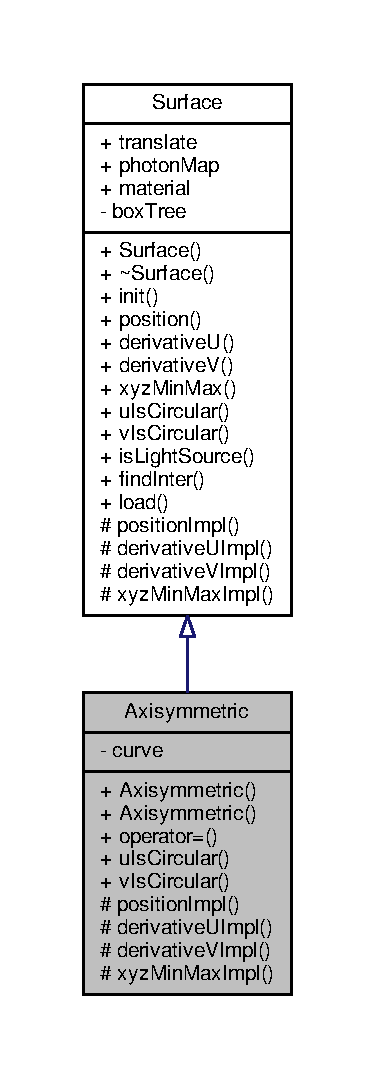
\includegraphics[width=180pt]{classAxisymmetric__inherit__graph}
\end{center}
\end{figure}


Collaboration diagram for Axisymmetric\+:
\nopagebreak
\begin{figure}[H]
\begin{center}
\leavevmode
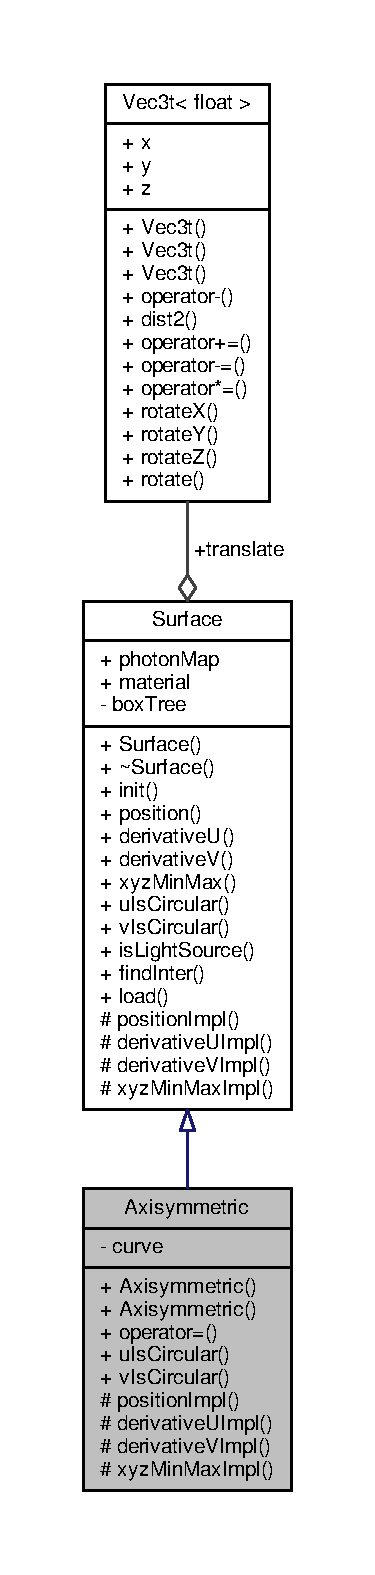
\includegraphics[height=550pt]{classAxisymmetric__coll__graph}
\end{center}
\end{figure}
\subsection*{Public Member Functions}
\begin{DoxyCompactItemize}
\item 
\hyperlink{classAxisymmetric_ab9470bf0bc24964f1c8b186d9e900036}{Axisymmetric} (const \hyperlink{classCurve}{Curve} $\ast$\+\_\+curve)
\item 
\hyperlink{classAxisymmetric_a3a9d954abfcb1bbb524382c9d64ae412}{Axisymmetric} (const \hyperlink{classAxisymmetric}{Axisymmetric} \&)=delete
\item 
\hyperlink{classAxisymmetric}{Axisymmetric} \& \hyperlink{classAxisymmetric_ab788a7e5b1f41fb28a128489cb0312d0}{operator=} (const \hyperlink{classAxisymmetric}{Axisymmetric} \&)=delete
\item 
bool \hyperlink{classAxisymmetric_a50b489a9914ad852638b586cc0c6c2dc}{u\+Is\+Circular} () const override
\item 
bool \hyperlink{classAxisymmetric_a63d63250b3ca2a34c2707abf35169657}{v\+Is\+Circular} () const override
\end{DoxyCompactItemize}
\subsection*{Protected Member Functions}
\begin{DoxyCompactItemize}
\item 
\hyperlink{vec_8h_ae4fcaa7c0a3935930ed1be5f70b90373}{Vec3} \hyperlink{classAxisymmetric_a65f503a73188b0647945bf3a6a5b901e}{position\+Impl} (float u, float v) const override
\begin{DoxyCompactList}\small\item\em Responsible to destroy it. \end{DoxyCompactList}\item 
\hyperlink{vec_8h_ae4fcaa7c0a3935930ed1be5f70b90373}{Vec3} \hyperlink{classAxisymmetric_a2af551bce6cffc034a278de5c2f5f3c4}{derivative\+U\+Impl} (float u, float v) const override
\item 
\hyperlink{vec_8h_ae4fcaa7c0a3935930ed1be5f70b90373}{Vec3} \hyperlink{classAxisymmetric_ab62630c58ba420d44eb39753f27abba9}{derivative\+V\+Impl} (float u, float v) const override
\item 
\hyperlink{structBox3}{Box3} \hyperlink{classAxisymmetric_a2718336bc4e05234a3f57bbe80ec29d3}{xyz\+Min\+Max\+Impl} (float u1, float u2, float v1, float v2) const override
\end{DoxyCompactItemize}
\subsection*{Private Attributes}
\begin{DoxyCompactItemize}
\item 
std\+::unique\+\_\+ptr$<$ const \hyperlink{classCurve}{Curve} $>$ \hyperlink{classAxisymmetric_a9786b5a7bc06ecb80325baf1193a92cc}{curve}
\end{DoxyCompactItemize}
\subsection*{Additional Inherited Members}


\subsection{Detailed Description}
Rotate a curve around z-\/axis to form a surface omega = u $\ast$ 2 $\ast$ PI, curve param = v \hyperlink{classCurve}{Curve(x, y)} =$>$ \hyperlink{classSurface}{Surface}(z, x $\sim$ y) If curve parameter v is positively correlated with x, normal goes outwards. 

\subsection{Constructor \& Destructor Documentation}
\index{Axisymmetric@{Axisymmetric}!Axisymmetric@{Axisymmetric}}
\index{Axisymmetric@{Axisymmetric}!Axisymmetric@{Axisymmetric}}
\subsubsection[{\texorpdfstring{Axisymmetric(const Curve $\ast$\+\_\+curve)}{Axisymmetric(const Curve *_curve)}}]{\setlength{\rightskip}{0pt plus 5cm}Axisymmetric\+::\+Axisymmetric (
\begin{DoxyParamCaption}
\item[{const {\bf Curve} $\ast$}]{\+\_\+curve}
\end{DoxyParamCaption}
)\hspace{0.3cm}{\ttfamily [inline]}}\hypertarget{classAxisymmetric_ab9470bf0bc24964f1c8b186d9e900036}{}\label{classAxisymmetric_ab9470bf0bc24964f1c8b186d9e900036}
\index{Axisymmetric@{Axisymmetric}!Axisymmetric@{Axisymmetric}}
\index{Axisymmetric@{Axisymmetric}!Axisymmetric@{Axisymmetric}}
\subsubsection[{\texorpdfstring{Axisymmetric(const Axisymmetric \&)=delete}{Axisymmetric(const Axisymmetric &)=delete}}]{\setlength{\rightskip}{0pt plus 5cm}Axisymmetric\+::\+Axisymmetric (
\begin{DoxyParamCaption}
\item[{const {\bf Axisymmetric} \&}]{}
\end{DoxyParamCaption}
)\hspace{0.3cm}{\ttfamily [delete]}}\hypertarget{classAxisymmetric_a3a9d954abfcb1bbb524382c9d64ae412}{}\label{classAxisymmetric_a3a9d954abfcb1bbb524382c9d64ae412}


\subsection{Member Function Documentation}
\index{Axisymmetric@{Axisymmetric}!derivative\+U\+Impl@{derivative\+U\+Impl}}
\index{derivative\+U\+Impl@{derivative\+U\+Impl}!Axisymmetric@{Axisymmetric}}
\subsubsection[{\texorpdfstring{derivative\+U\+Impl(float u, float v) const override}{derivativeUImpl(float u, float v) const override}}]{\setlength{\rightskip}{0pt plus 5cm}{\bf Vec3} Axisymmetric\+::derivative\+U\+Impl (
\begin{DoxyParamCaption}
\item[{float}]{u, }
\item[{float}]{v}
\end{DoxyParamCaption}
) const\hspace{0.3cm}{\ttfamily [inline]}, {\ttfamily [override]}, {\ttfamily [protected]}, {\ttfamily [virtual]}}\hypertarget{classAxisymmetric_a2af551bce6cffc034a278de5c2f5f3c4}{}\label{classAxisymmetric_a2af551bce6cffc034a278de5c2f5f3c4}


Implements \hyperlink{classSurface_a4de8fb9d4652cc32022c95eb903cce4a}{Surface}.

\index{Axisymmetric@{Axisymmetric}!derivative\+V\+Impl@{derivative\+V\+Impl}}
\index{derivative\+V\+Impl@{derivative\+V\+Impl}!Axisymmetric@{Axisymmetric}}
\subsubsection[{\texorpdfstring{derivative\+V\+Impl(float u, float v) const override}{derivativeVImpl(float u, float v) const override}}]{\setlength{\rightskip}{0pt plus 5cm}{\bf Vec3} Axisymmetric\+::derivative\+V\+Impl (
\begin{DoxyParamCaption}
\item[{float}]{u, }
\item[{float}]{v}
\end{DoxyParamCaption}
) const\hspace{0.3cm}{\ttfamily [inline]}, {\ttfamily [override]}, {\ttfamily [protected]}, {\ttfamily [virtual]}}\hypertarget{classAxisymmetric_ab62630c58ba420d44eb39753f27abba9}{}\label{classAxisymmetric_ab62630c58ba420d44eb39753f27abba9}


Implements \hyperlink{classSurface_a95d65437419ba8d439fa8f0d71f963a1}{Surface}.

\index{Axisymmetric@{Axisymmetric}!operator=@{operator=}}
\index{operator=@{operator=}!Axisymmetric@{Axisymmetric}}
\subsubsection[{\texorpdfstring{operator=(const Axisymmetric \&)=delete}{operator=(const Axisymmetric &)=delete}}]{\setlength{\rightskip}{0pt plus 5cm}{\bf Axisymmetric}\& Axisymmetric\+::operator= (
\begin{DoxyParamCaption}
\item[{const {\bf Axisymmetric} \&}]{}
\end{DoxyParamCaption}
)\hspace{0.3cm}{\ttfamily [delete]}}\hypertarget{classAxisymmetric_ab788a7e5b1f41fb28a128489cb0312d0}{}\label{classAxisymmetric_ab788a7e5b1f41fb28a128489cb0312d0}
\index{Axisymmetric@{Axisymmetric}!position\+Impl@{position\+Impl}}
\index{position\+Impl@{position\+Impl}!Axisymmetric@{Axisymmetric}}
\subsubsection[{\texorpdfstring{position\+Impl(float u, float v) const override}{positionImpl(float u, float v) const override}}]{\setlength{\rightskip}{0pt plus 5cm}{\bf Vec3} Axisymmetric\+::position\+Impl (
\begin{DoxyParamCaption}
\item[{float}]{u, }
\item[{float}]{v}
\end{DoxyParamCaption}
) const\hspace{0.3cm}{\ttfamily [inline]}, {\ttfamily [override]}, {\ttfamily [protected]}, {\ttfamily [virtual]}}\hypertarget{classAxisymmetric_a65f503a73188b0647945bf3a6a5b901e}{}\label{classAxisymmetric_a65f503a73188b0647945bf3a6a5b901e}


Responsible to destroy it. 



Implements \hyperlink{classSurface_a379545eea4809f81fe7e037f5e5ff4be}{Surface}.

\index{Axisymmetric@{Axisymmetric}!u\+Is\+Circular@{u\+Is\+Circular}}
\index{u\+Is\+Circular@{u\+Is\+Circular}!Axisymmetric@{Axisymmetric}}
\subsubsection[{\texorpdfstring{u\+Is\+Circular() const override}{uIsCircular() const override}}]{\setlength{\rightskip}{0pt plus 5cm}bool Axisymmetric\+::u\+Is\+Circular (
\begin{DoxyParamCaption}
{}
\end{DoxyParamCaption}
) const\hspace{0.3cm}{\ttfamily [inline]}, {\ttfamily [override]}, {\ttfamily [virtual]}}\hypertarget{classAxisymmetric_a50b489a9914ad852638b586cc0c6c2dc}{}\label{classAxisymmetric_a50b489a9914ad852638b586cc0c6c2dc}


Implements \hyperlink{classSurface_a11d5759ec3e3d43036fb949dcc6f5562}{Surface}.

\index{Axisymmetric@{Axisymmetric}!v\+Is\+Circular@{v\+Is\+Circular}}
\index{v\+Is\+Circular@{v\+Is\+Circular}!Axisymmetric@{Axisymmetric}}
\subsubsection[{\texorpdfstring{v\+Is\+Circular() const override}{vIsCircular() const override}}]{\setlength{\rightskip}{0pt plus 5cm}bool Axisymmetric\+::v\+Is\+Circular (
\begin{DoxyParamCaption}
{}
\end{DoxyParamCaption}
) const\hspace{0.3cm}{\ttfamily [inline]}, {\ttfamily [override]}, {\ttfamily [virtual]}}\hypertarget{classAxisymmetric_a63d63250b3ca2a34c2707abf35169657}{}\label{classAxisymmetric_a63d63250b3ca2a34c2707abf35169657}


Implements \hyperlink{classSurface_af52f9322929a702a9aaeee3ae4a368da}{Surface}.

\index{Axisymmetric@{Axisymmetric}!xyz\+Min\+Max\+Impl@{xyz\+Min\+Max\+Impl}}
\index{xyz\+Min\+Max\+Impl@{xyz\+Min\+Max\+Impl}!Axisymmetric@{Axisymmetric}}
\subsubsection[{\texorpdfstring{xyz\+Min\+Max\+Impl(float u1, float u2, float v1, float v2) const override}{xyzMinMaxImpl(float u1, float u2, float v1, float v2) const override}}]{\setlength{\rightskip}{0pt plus 5cm}{\bf Box3} Axisymmetric\+::xyz\+Min\+Max\+Impl (
\begin{DoxyParamCaption}
\item[{float}]{u1, }
\item[{float}]{u2, }
\item[{float}]{v1, }
\item[{float}]{v2}
\end{DoxyParamCaption}
) const\hspace{0.3cm}{\ttfamily [inline]}, {\ttfamily [override]}, {\ttfamily [protected]}, {\ttfamily [virtual]}}\hypertarget{classAxisymmetric_a2718336bc4e05234a3f57bbe80ec29d3}{}\label{classAxisymmetric_a2718336bc4e05234a3f57bbe80ec29d3}


Implements \hyperlink{classSurface_ab1ee990da290748cd86aaf95edb28c38}{Surface}.



\subsection{Member Data Documentation}
\index{Axisymmetric@{Axisymmetric}!curve@{curve}}
\index{curve@{curve}!Axisymmetric@{Axisymmetric}}
\subsubsection[{\texorpdfstring{curve}{curve}}]{\setlength{\rightskip}{0pt plus 5cm}std\+::unique\+\_\+ptr$<$const {\bf Curve}$>$ Axisymmetric\+::curve\hspace{0.3cm}{\ttfamily [private]}}\hypertarget{classAxisymmetric_a9786b5a7bc06ecb80325baf1193a92cc}{}\label{classAxisymmetric_a9786b5a7bc06ecb80325baf1193a92cc}


The documentation for this class was generated from the following file\+:\begin{DoxyCompactItemize}
\item 
\hyperlink{axisymmetric_8h}{axisymmetric.\+h}\end{DoxyCompactItemize}

\hypertarget{classBezier3}{}\section{Bezier3 Class Reference}
\label{classBezier3}\index{Bezier3@{Bezier3}}


3-\/dgree Bezier \hyperlink{classCurve}{Curve}  




{\ttfamily \#include $<$bezier3.\+h$>$}



Inheritance diagram for Bezier3\+:\nopagebreak
\begin{figure}[H]
\begin{center}
\leavevmode
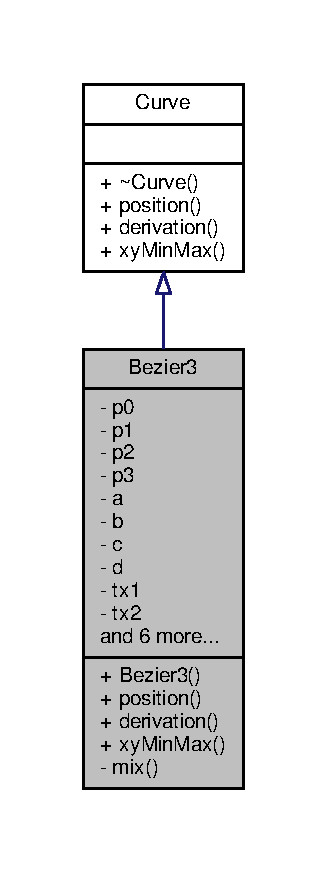
\includegraphics[width=157pt]{classBezier3__inherit__graph}
\end{center}
\end{figure}


Collaboration diagram for Bezier3\+:\nopagebreak
\begin{figure}[H]
\begin{center}
\leavevmode
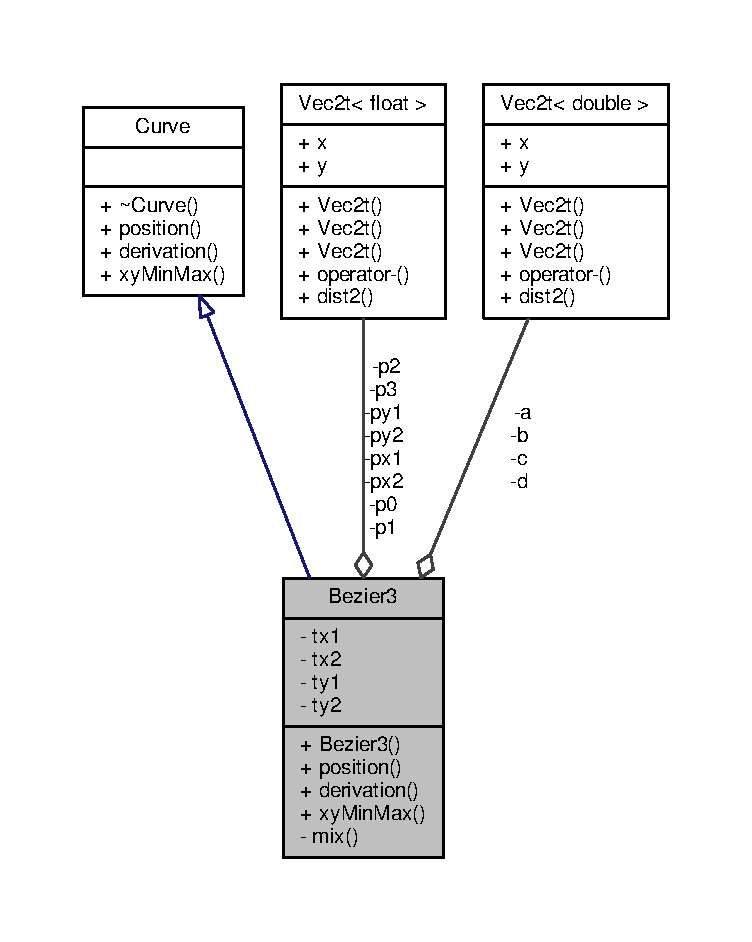
\includegraphics[width=350pt]{classBezier3__coll__graph}
\end{center}
\end{figure}
\subsection*{Public Member Functions}
\begin{DoxyCompactItemize}
\item 
\hyperlink{classBezier3_a7ecadca050fc7935c58c67de8b767dcf}{Bezier3} (const \hyperlink{vec_8h_a871640c4eb6057d21b25824c55250629}{Vec2} \&\+\_\+p0, const \hyperlink{vec_8h_a871640c4eb6057d21b25824c55250629}{Vec2} \&\+\_\+p1, const \hyperlink{vec_8h_a871640c4eb6057d21b25824c55250629}{Vec2} \&\+\_\+p2, const \hyperlink{vec_8h_a871640c4eb6057d21b25824c55250629}{Vec2} \&\+\_\+p3)
\begin{DoxyCompactList}\small\item\em Extream value for x and y. \end{DoxyCompactList}\item 
\hyperlink{vec_8h_a871640c4eb6057d21b25824c55250629}{Vec2} \hyperlink{classBezier3_afd1907f62d8d19b4683f43080a0334db}{position} (float t) const override
\begin{DoxyCompactList}\small\item\em Get point on the curve. \end{DoxyCompactList}\item 
\hyperlink{vec_8h_a871640c4eb6057d21b25824c55250629}{Vec2} \hyperlink{classBezier3_a8f3bc3ba14dae6e9f27366ef587accc5}{derivation} (float t) const override
\begin{DoxyCompactList}\small\item\em Get derivation. \end{DoxyCompactList}\item 
\hyperlink{structBox2}{Box2} \hyperlink{classBezier3_aa5a1d33483071204f99774fefb092caf}{xy\+Min\+Max} (float t1, float t2) const override
\begin{DoxyCompactList}\small\item\em (x\+:(min, max), y\+:(min, max)) when t in \mbox{[}x1, x2\mbox{]} \end{DoxyCompactList}\end{DoxyCompactItemize}
\subsection*{Static Private Member Functions}
\begin{DoxyCompactItemize}
\item 
static \hyperlink{vec_8h_a871640c4eb6057d21b25824c55250629}{Vec2} \hyperlink{classBezier3_a023a628ce0ed0750b3bf9c00086843aa}{mix} (const \hyperlink{vec_8h_a871640c4eb6057d21b25824c55250629}{Vec2} \&v1, const \hyperlink{vec_8h_a871640c4eb6057d21b25824c55250629}{Vec2} \&v2, float k)
\end{DoxyCompactItemize}
\subsection*{Private Attributes}
\begin{DoxyCompactItemize}
\item 
\hyperlink{vec_8h_a871640c4eb6057d21b25824c55250629}{Vec2} \hyperlink{classBezier3_a61297313c61fc20a334b12603f59b999}{p0}
\item 
\hyperlink{vec_8h_a871640c4eb6057d21b25824c55250629}{Vec2} \hyperlink{classBezier3_acad9cdcdafe19feef1002ced52099cfe}{p1}
\item 
\hyperlink{vec_8h_a871640c4eb6057d21b25824c55250629}{Vec2} \hyperlink{classBezier3_aa78aee06abc3a06c2dd636df4fe4451d}{p2}
\item 
\hyperlink{vec_8h_a871640c4eb6057d21b25824c55250629}{Vec2} \hyperlink{classBezier3_a0e1e35eb084266b2dcd71ecf9b19b80f}{p3}
\item 
\hyperlink{structVec2t}{Vec2t}$<$ double $>$ \hyperlink{classBezier3_ae83be4ce590bf7a7a2bf53adeeb170cf}{a}
\item 
\hyperlink{structVec2t}{Vec2t}$<$ double $>$ \hyperlink{classBezier3_ad63b9a75228af1727b61fe032f7e2f68}{b}
\item 
\hyperlink{structVec2t}{Vec2t}$<$ double $>$ \hyperlink{classBezier3_aafb4270797f10af53a7feba1a66d59a0}{c}
\item 
\hyperlink{structVec2t}{Vec2t}$<$ double $>$ \hyperlink{classBezier3_a5ce0d6743e932b0096b64804324dad9b}{d}
\item 
float \hyperlink{classBezier3_ac017ccb0ddaadd93fcb65e144abfab64}{tx1}
\begin{DoxyCompactList}\small\item\em Expanded polynomial coefficient. \end{DoxyCompactList}\item 
float \hyperlink{classBezier3_a167a03a8686c66095e36c86b1ce2eef0}{tx2}
\item 
float \hyperlink{classBezier3_ad4f47c85e457139bd3f9e344b72309c1}{ty1}
\item 
float \hyperlink{classBezier3_aa956edaaef544c1ef270a0e5f9e333f2}{ty2}
\item 
\hyperlink{vec_8h_a871640c4eb6057d21b25824c55250629}{Vec2} \hyperlink{classBezier3_a7d69e4d349bbe7a7351188d2c0a3ef4b}{px1}
\begin{DoxyCompactList}\small\item\em Coresponding t for extream values. \end{DoxyCompactList}\item 
\hyperlink{vec_8h_a871640c4eb6057d21b25824c55250629}{Vec2} \hyperlink{classBezier3_ae439178d68735ec771c72d097cb90997}{px2}
\item 
\hyperlink{vec_8h_a871640c4eb6057d21b25824c55250629}{Vec2} \hyperlink{classBezier3_a6bdba56f87b7c2f2fd32361cd0cccdc8}{py1}
\item 
\hyperlink{vec_8h_a871640c4eb6057d21b25824c55250629}{Vec2} \hyperlink{classBezier3_affcc44acee6b341088cdd403c55fa61e}{py2}
\end{DoxyCompactItemize}


\subsection{Detailed Description}
3-\/dgree Bezier \hyperlink{classCurve}{Curve} 

\subsection{Constructor \& Destructor Documentation}
\index{Bezier3@{Bezier3}!Bezier3@{Bezier3}}
\index{Bezier3@{Bezier3}!Bezier3@{Bezier3}}
\subsubsection[{\texorpdfstring{Bezier3(const Vec2 \&\+\_\+p0, const Vec2 \&\+\_\+p1, const Vec2 \&\+\_\+p2, const Vec2 \&\+\_\+p3)}{Bezier3(const Vec2 &_p0, const Vec2 &_p1, const Vec2 &_p2, const Vec2 &_p3)}}]{\setlength{\rightskip}{0pt plus 5cm}Bezier3\+::\+Bezier3 (
\begin{DoxyParamCaption}
\item[{const {\bf Vec2} \&}]{\+\_\+p0, }
\item[{const {\bf Vec2} \&}]{\+\_\+p1, }
\item[{const {\bf Vec2} \&}]{\+\_\+p2, }
\item[{const {\bf Vec2} \&}]{\+\_\+p3}
\end{DoxyParamCaption}
)\hspace{0.3cm}{\ttfamily [inline]}}\hypertarget{classBezier3_a7ecadca050fc7935c58c67de8b767dcf}{}\label{classBezier3_a7ecadca050fc7935c58c67de8b767dcf}


Extream value for x and y. 

Construct with 4 control points Subtracting similar numbers decreses accuracy, so use double 

\subsection{Member Function Documentation}
\index{Bezier3@{Bezier3}!derivation@{derivation}}
\index{derivation@{derivation}!Bezier3@{Bezier3}}
\subsubsection[{\texorpdfstring{derivation(float t) const override}{derivation(float t) const override}}]{\setlength{\rightskip}{0pt plus 5cm}{\bf Vec2} Bezier3\+::derivation (
\begin{DoxyParamCaption}
\item[{float}]{t}
\end{DoxyParamCaption}
) const\hspace{0.3cm}{\ttfamily [inline]}, {\ttfamily [override]}, {\ttfamily [virtual]}}\hypertarget{classBezier3_a8f3bc3ba14dae6e9f27366ef587accc5}{}\label{classBezier3_a8f3bc3ba14dae6e9f27366ef587accc5}


Get derivation. 



Implements \hyperlink{classCurve_acca6db6f7d2f45fbea676db16e3784be}{Curve}.

\index{Bezier3@{Bezier3}!mix@{mix}}
\index{mix@{mix}!Bezier3@{Bezier3}}
\subsubsection[{\texorpdfstring{mix(const Vec2 \&v1, const Vec2 \&v2, float k)}{mix(const Vec2 &v1, const Vec2 &v2, float k)}}]{\setlength{\rightskip}{0pt plus 5cm}{\bf Vec2} Bezier3\+::mix (
\begin{DoxyParamCaption}
\item[{const {\bf Vec2} \&}]{v1, }
\item[{const {\bf Vec2} \&}]{v2, }
\item[{float}]{k}
\end{DoxyParamCaption}
)\hspace{0.3cm}{\ttfamily [inline]}, {\ttfamily [static]}, {\ttfamily [private]}}\hypertarget{classBezier3_a023a628ce0ed0750b3bf9c00086843aa}{}\label{classBezier3_a023a628ce0ed0750b3bf9c00086843aa}
\index{Bezier3@{Bezier3}!position@{position}}
\index{position@{position}!Bezier3@{Bezier3}}
\subsubsection[{\texorpdfstring{position(float t) const override}{position(float t) const override}}]{\setlength{\rightskip}{0pt plus 5cm}{\bf Vec2} Bezier3\+::position (
\begin{DoxyParamCaption}
\item[{float}]{t}
\end{DoxyParamCaption}
) const\hspace{0.3cm}{\ttfamily [inline]}, {\ttfamily [override]}, {\ttfamily [virtual]}}\hypertarget{classBezier3_afd1907f62d8d19b4683f43080a0334db}{}\label{classBezier3_afd1907f62d8d19b4683f43080a0334db}


Get point on the curve. 



Implements \hyperlink{classCurve_a919ea6d17b6fc0dc6ea6facec6d5623c}{Curve}.

\index{Bezier3@{Bezier3}!xy\+Min\+Max@{xy\+Min\+Max}}
\index{xy\+Min\+Max@{xy\+Min\+Max}!Bezier3@{Bezier3}}
\subsubsection[{\texorpdfstring{xy\+Min\+Max(float t1, float t2) const override}{xyMinMax(float t1, float t2) const override}}]{\setlength{\rightskip}{0pt plus 5cm}{\bf Box2} Bezier3\+::xy\+Min\+Max (
\begin{DoxyParamCaption}
\item[{float}]{t1, }
\item[{float}]{t2}
\end{DoxyParamCaption}
) const\hspace{0.3cm}{\ttfamily [inline]}, {\ttfamily [override]}, {\ttfamily [virtual]}}\hypertarget{classBezier3_aa5a1d33483071204f99774fefb092caf}{}\label{classBezier3_aa5a1d33483071204f99774fefb092caf}


(x\+:(min, max), y\+:(min, max)) when t in \mbox{[}x1, x2\mbox{]} 



Implements \hyperlink{classCurve_add48a303ee076bfce08340dd1241cbf6}{Curve}.



\subsection{Member Data Documentation}
\index{Bezier3@{Bezier3}!a@{a}}
\index{a@{a}!Bezier3@{Bezier3}}
\subsubsection[{\texorpdfstring{a}{a}}]{\setlength{\rightskip}{0pt plus 5cm}{\bf Vec2t}$<$double$>$ Bezier3\+::a\hspace{0.3cm}{\ttfamily [private]}}\hypertarget{classBezier3_ae83be4ce590bf7a7a2bf53adeeb170cf}{}\label{classBezier3_ae83be4ce590bf7a7a2bf53adeeb170cf}
\index{Bezier3@{Bezier3}!b@{b}}
\index{b@{b}!Bezier3@{Bezier3}}
\subsubsection[{\texorpdfstring{b}{b}}]{\setlength{\rightskip}{0pt plus 5cm}{\bf Vec2t}$<$double$>$ Bezier3\+::b\hspace{0.3cm}{\ttfamily [private]}}\hypertarget{classBezier3_ad63b9a75228af1727b61fe032f7e2f68}{}\label{classBezier3_ad63b9a75228af1727b61fe032f7e2f68}
\index{Bezier3@{Bezier3}!c@{c}}
\index{c@{c}!Bezier3@{Bezier3}}
\subsubsection[{\texorpdfstring{c}{c}}]{\setlength{\rightskip}{0pt plus 5cm}{\bf Vec2t}$<$double$>$ Bezier3\+::c\hspace{0.3cm}{\ttfamily [private]}}\hypertarget{classBezier3_aafb4270797f10af53a7feba1a66d59a0}{}\label{classBezier3_aafb4270797f10af53a7feba1a66d59a0}
\index{Bezier3@{Bezier3}!d@{d}}
\index{d@{d}!Bezier3@{Bezier3}}
\subsubsection[{\texorpdfstring{d}{d}}]{\setlength{\rightskip}{0pt plus 5cm}{\bf Vec2t}$<$double$>$ Bezier3\+::d\hspace{0.3cm}{\ttfamily [private]}}\hypertarget{classBezier3_a5ce0d6743e932b0096b64804324dad9b}{}\label{classBezier3_a5ce0d6743e932b0096b64804324dad9b}
\index{Bezier3@{Bezier3}!p0@{p0}}
\index{p0@{p0}!Bezier3@{Bezier3}}
\subsubsection[{\texorpdfstring{p0}{p0}}]{\setlength{\rightskip}{0pt plus 5cm}{\bf Vec2} Bezier3\+::p0\hspace{0.3cm}{\ttfamily [private]}}\hypertarget{classBezier3_a61297313c61fc20a334b12603f59b999}{}\label{classBezier3_a61297313c61fc20a334b12603f59b999}
\index{Bezier3@{Bezier3}!p1@{p1}}
\index{p1@{p1}!Bezier3@{Bezier3}}
\subsubsection[{\texorpdfstring{p1}{p1}}]{\setlength{\rightskip}{0pt plus 5cm}{\bf Vec2} Bezier3\+::p1\hspace{0.3cm}{\ttfamily [private]}}\hypertarget{classBezier3_acad9cdcdafe19feef1002ced52099cfe}{}\label{classBezier3_acad9cdcdafe19feef1002ced52099cfe}
\index{Bezier3@{Bezier3}!p2@{p2}}
\index{p2@{p2}!Bezier3@{Bezier3}}
\subsubsection[{\texorpdfstring{p2}{p2}}]{\setlength{\rightskip}{0pt plus 5cm}{\bf Vec2} Bezier3\+::p2\hspace{0.3cm}{\ttfamily [private]}}\hypertarget{classBezier3_aa78aee06abc3a06c2dd636df4fe4451d}{}\label{classBezier3_aa78aee06abc3a06c2dd636df4fe4451d}
\index{Bezier3@{Bezier3}!p3@{p3}}
\index{p3@{p3}!Bezier3@{Bezier3}}
\subsubsection[{\texorpdfstring{p3}{p3}}]{\setlength{\rightskip}{0pt plus 5cm}{\bf Vec2} Bezier3\+::p3\hspace{0.3cm}{\ttfamily [private]}}\hypertarget{classBezier3_a0e1e35eb084266b2dcd71ecf9b19b80f}{}\label{classBezier3_a0e1e35eb084266b2dcd71ecf9b19b80f}
\index{Bezier3@{Bezier3}!px1@{px1}}
\index{px1@{px1}!Bezier3@{Bezier3}}
\subsubsection[{\texorpdfstring{px1}{px1}}]{\setlength{\rightskip}{0pt plus 5cm}{\bf Vec2} Bezier3\+::px1\hspace{0.3cm}{\ttfamily [private]}}\hypertarget{classBezier3_a7d69e4d349bbe7a7351188d2c0a3ef4b}{}\label{classBezier3_a7d69e4d349bbe7a7351188d2c0a3ef4b}


Coresponding t for extream values. 

\index{Bezier3@{Bezier3}!px2@{px2}}
\index{px2@{px2}!Bezier3@{Bezier3}}
\subsubsection[{\texorpdfstring{px2}{px2}}]{\setlength{\rightskip}{0pt plus 5cm}{\bf Vec2} Bezier3\+::px2\hspace{0.3cm}{\ttfamily [private]}}\hypertarget{classBezier3_ae439178d68735ec771c72d097cb90997}{}\label{classBezier3_ae439178d68735ec771c72d097cb90997}
\index{Bezier3@{Bezier3}!py1@{py1}}
\index{py1@{py1}!Bezier3@{Bezier3}}
\subsubsection[{\texorpdfstring{py1}{py1}}]{\setlength{\rightskip}{0pt plus 5cm}{\bf Vec2} Bezier3\+::py1\hspace{0.3cm}{\ttfamily [private]}}\hypertarget{classBezier3_a6bdba56f87b7c2f2fd32361cd0cccdc8}{}\label{classBezier3_a6bdba56f87b7c2f2fd32361cd0cccdc8}
\index{Bezier3@{Bezier3}!py2@{py2}}
\index{py2@{py2}!Bezier3@{Bezier3}}
\subsubsection[{\texorpdfstring{py2}{py2}}]{\setlength{\rightskip}{0pt plus 5cm}{\bf Vec2} Bezier3\+::py2\hspace{0.3cm}{\ttfamily [private]}}\hypertarget{classBezier3_affcc44acee6b341088cdd403c55fa61e}{}\label{classBezier3_affcc44acee6b341088cdd403c55fa61e}
\index{Bezier3@{Bezier3}!tx1@{tx1}}
\index{tx1@{tx1}!Bezier3@{Bezier3}}
\subsubsection[{\texorpdfstring{tx1}{tx1}}]{\setlength{\rightskip}{0pt plus 5cm}float Bezier3\+::tx1\hspace{0.3cm}{\ttfamily [private]}}\hypertarget{classBezier3_ac017ccb0ddaadd93fcb65e144abfab64}{}\label{classBezier3_ac017ccb0ddaadd93fcb65e144abfab64}


Expanded polynomial coefficient. 

\index{Bezier3@{Bezier3}!tx2@{tx2}}
\index{tx2@{tx2}!Bezier3@{Bezier3}}
\subsubsection[{\texorpdfstring{tx2}{tx2}}]{\setlength{\rightskip}{0pt plus 5cm}float Bezier3\+::tx2\hspace{0.3cm}{\ttfamily [private]}}\hypertarget{classBezier3_a167a03a8686c66095e36c86b1ce2eef0}{}\label{classBezier3_a167a03a8686c66095e36c86b1ce2eef0}
\index{Bezier3@{Bezier3}!ty1@{ty1}}
\index{ty1@{ty1}!Bezier3@{Bezier3}}
\subsubsection[{\texorpdfstring{ty1}{ty1}}]{\setlength{\rightskip}{0pt plus 5cm}float Bezier3\+::ty1\hspace{0.3cm}{\ttfamily [private]}}\hypertarget{classBezier3_ad4f47c85e457139bd3f9e344b72309c1}{}\label{classBezier3_ad4f47c85e457139bd3f9e344b72309c1}
\index{Bezier3@{Bezier3}!ty2@{ty2}}
\index{ty2@{ty2}!Bezier3@{Bezier3}}
\subsubsection[{\texorpdfstring{ty2}{ty2}}]{\setlength{\rightskip}{0pt plus 5cm}float Bezier3\+::ty2\hspace{0.3cm}{\ttfamily [private]}}\hypertarget{classBezier3_aa956edaaef544c1ef270a0e5f9e333f2}{}\label{classBezier3_aa956edaaef544c1ef270a0e5f9e333f2}


The documentation for this class was generated from the following file\+:\begin{DoxyCompactItemize}
\item 
\hyperlink{bezier3_8h}{bezier3.\+h}\end{DoxyCompactItemize}

\hypertarget{structBox2}{}\section{Box2 Struct Reference}
\label{structBox2}\index{Box2@{Box2}}


{\ttfamily \#include $<$box.\+h$>$}



Collaboration diagram for Box2\+:\nopagebreak
\begin{figure}[H]
\begin{center}
\leavevmode
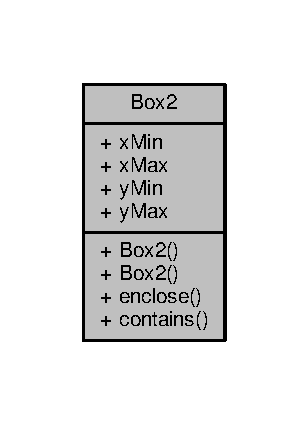
\includegraphics[width=148pt]{structBox2__coll__graph}
\end{center}
\end{figure}
\subsection*{Public Member Functions}
\begin{DoxyCompactItemize}
\item 
\hyperlink{structBox2_a6aa87f2d8b412ea27e6d21e6d14ea82e}{Box2} (float \+\_\+x\+Min, float \+\_\+x\+Max, float \+\_\+y\+Min, float \+\_\+y\+Max)
\item 
\hyperlink{structBox2_a5c4aa39e6462fdd31744eac9118b85a2}{Box2} (\hyperlink{vec_8h_a871640c4eb6057d21b25824c55250629}{Vec2} p1, \hyperlink{vec_8h_a871640c4eb6057d21b25824c55250629}{Vec2} p2)
\item 
void \hyperlink{structBox2_a7c79861eb4a94933f7facebfb53d44b2}{enclose} (\hyperlink{vec_8h_a871640c4eb6057d21b25824c55250629}{Vec2} p)
\item 
bool \hyperlink{structBox2_ad32f112b01ce71919b93b7bda4aec775}{contains} (const \hyperlink{vec_8h_a871640c4eb6057d21b25824c55250629}{Vec2} \&v) const 
\begin{DoxyCompactList}\small\item\em Containing includes falling nearing the edge. \end{DoxyCompactList}\end{DoxyCompactItemize}
\subsection*{Public Attributes}
\begin{DoxyCompactItemize}
\item 
float \hyperlink{structBox2_a99630f8c30f5c15831e86b009bca148d}{x\+Min}
\item 
float \hyperlink{structBox2_acbcaadab1ce72ba9cb01616ed356ac5c}{x\+Max}
\item 
float \hyperlink{structBox2_ac5081aaad7feba1664d76fc42ea307d7}{y\+Min}
\item 
float \hyperlink{structBox2_ab40c4b0a0b8c510402b97a16ece7fd58}{y\+Max}
\end{DoxyCompactItemize}


\subsection{Constructor \& Destructor Documentation}
\index{Box2@{Box2}!Box2@{Box2}}
\index{Box2@{Box2}!Box2@{Box2}}
\subsubsection[{\texorpdfstring{Box2(float \+\_\+x\+Min, float \+\_\+x\+Max, float \+\_\+y\+Min, float \+\_\+y\+Max)}{Box2(float _xMin, float _xMax, float _yMin, float _yMax)}}]{\setlength{\rightskip}{0pt plus 5cm}Box2\+::\+Box2 (
\begin{DoxyParamCaption}
\item[{float}]{\+\_\+x\+Min, }
\item[{float}]{\+\_\+x\+Max, }
\item[{float}]{\+\_\+y\+Min, }
\item[{float}]{\+\_\+y\+Max}
\end{DoxyParamCaption}
)\hspace{0.3cm}{\ttfamily [inline]}}\hypertarget{structBox2_a6aa87f2d8b412ea27e6d21e6d14ea82e}{}\label{structBox2_a6aa87f2d8b412ea27e6d21e6d14ea82e}
\index{Box2@{Box2}!Box2@{Box2}}
\index{Box2@{Box2}!Box2@{Box2}}
\subsubsection[{\texorpdfstring{Box2(\+Vec2 p1, Vec2 p2)}{Box2(Vec2 p1, Vec2 p2)}}]{\setlength{\rightskip}{0pt plus 5cm}Box2\+::\+Box2 (
\begin{DoxyParamCaption}
\item[{{\bf Vec2}}]{p1, }
\item[{{\bf Vec2}}]{p2}
\end{DoxyParamCaption}
)\hspace{0.3cm}{\ttfamily [inline]}}\hypertarget{structBox2_a5c4aa39e6462fdd31744eac9118b85a2}{}\label{structBox2_a5c4aa39e6462fdd31744eac9118b85a2}


\subsection{Member Function Documentation}
\index{Box2@{Box2}!contains@{contains}}
\index{contains@{contains}!Box2@{Box2}}
\subsubsection[{\texorpdfstring{contains(const Vec2 \&v) const }{contains(const Vec2 &v) const }}]{\setlength{\rightskip}{0pt plus 5cm}bool Box2\+::contains (
\begin{DoxyParamCaption}
\item[{const {\bf Vec2} \&}]{v}
\end{DoxyParamCaption}
) const\hspace{0.3cm}{\ttfamily [inline]}}\hypertarget{structBox2_ad32f112b01ce71919b93b7bda4aec775}{}\label{structBox2_ad32f112b01ce71919b93b7bda4aec775}


Containing includes falling nearing the edge. 

\index{Box2@{Box2}!enclose@{enclose}}
\index{enclose@{enclose}!Box2@{Box2}}
\subsubsection[{\texorpdfstring{enclose(\+Vec2 p)}{enclose(Vec2 p)}}]{\setlength{\rightskip}{0pt plus 5cm}void Box2\+::enclose (
\begin{DoxyParamCaption}
\item[{{\bf Vec2}}]{p}
\end{DoxyParamCaption}
)\hspace{0.3cm}{\ttfamily [inline]}}\hypertarget{structBox2_a7c79861eb4a94933f7facebfb53d44b2}{}\label{structBox2_a7c79861eb4a94933f7facebfb53d44b2}


\subsection{Member Data Documentation}
\index{Box2@{Box2}!x\+Max@{x\+Max}}
\index{x\+Max@{x\+Max}!Box2@{Box2}}
\subsubsection[{\texorpdfstring{x\+Max}{xMax}}]{\setlength{\rightskip}{0pt plus 5cm}float Box2\+::x\+Max}\hypertarget{structBox2_acbcaadab1ce72ba9cb01616ed356ac5c}{}\label{structBox2_acbcaadab1ce72ba9cb01616ed356ac5c}
\index{Box2@{Box2}!x\+Min@{x\+Min}}
\index{x\+Min@{x\+Min}!Box2@{Box2}}
\subsubsection[{\texorpdfstring{x\+Min}{xMin}}]{\setlength{\rightskip}{0pt plus 5cm}float Box2\+::x\+Min}\hypertarget{structBox2_a99630f8c30f5c15831e86b009bca148d}{}\label{structBox2_a99630f8c30f5c15831e86b009bca148d}
\index{Box2@{Box2}!y\+Max@{y\+Max}}
\index{y\+Max@{y\+Max}!Box2@{Box2}}
\subsubsection[{\texorpdfstring{y\+Max}{yMax}}]{\setlength{\rightskip}{0pt plus 5cm}float Box2\+::y\+Max}\hypertarget{structBox2_ab40c4b0a0b8c510402b97a16ece7fd58}{}\label{structBox2_ab40c4b0a0b8c510402b97a16ece7fd58}
\index{Box2@{Box2}!y\+Min@{y\+Min}}
\index{y\+Min@{y\+Min}!Box2@{Box2}}
\subsubsection[{\texorpdfstring{y\+Min}{yMin}}]{\setlength{\rightskip}{0pt plus 5cm}float Box2\+::y\+Min}\hypertarget{structBox2_ac5081aaad7feba1664d76fc42ea307d7}{}\label{structBox2_ac5081aaad7feba1664d76fc42ea307d7}


The documentation for this struct was generated from the following file\+:\begin{DoxyCompactItemize}
\item 
\hyperlink{box_8h}{box.\+h}\end{DoxyCompactItemize}

\hypertarget{structBox3}{}\section{Box3 Struct Reference}
\label{structBox3}\index{Box3@{Box3}}


{\ttfamily \#include $<$box.\+h$>$}



Collaboration diagram for Box3\+:\nopagebreak
\begin{figure}[H]
\begin{center}
\leavevmode
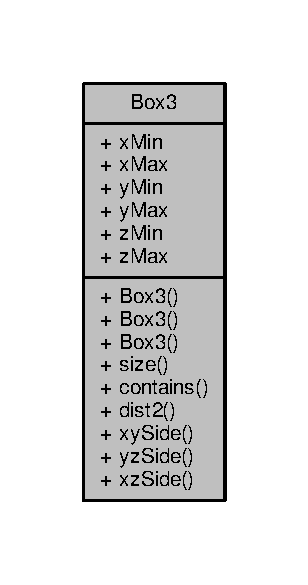
\includegraphics[width=148pt]{structBox3__coll__graph}
\end{center}
\end{figure}
\subsection*{Public Member Functions}
\begin{DoxyCompactItemize}
\item 
\hyperlink{structBox3_a01c66e99dab9c1316365b51f57b1bdb6}{Box3} ()
\item 
\hyperlink{structBox3_af368463aef860568bfe9592838d36571}{Box3} (float \+\_\+x\+Min, float \+\_\+x\+Max, float \+\_\+y\+Min, float \+\_\+y\+Max, float \+\_\+z\+Min, float \+\_\+z\+Max)
\item 
\hyperlink{structBox3_a4a326b1695b4dc2488cbb41a428ad8c1}{Box3} (const \hyperlink{vec_8h_ae4fcaa7c0a3935930ed1be5f70b90373}{Vec3} \&v)
\item 
float \hyperlink{structBox3_aa78365c1573abce91e6584addcbc686e}{size} () const 
\item 
bool \hyperlink{structBox3_a45cc24b44a662f9e7fee59437acb488b}{contains} (const \hyperlink{vec_8h_ae4fcaa7c0a3935930ed1be5f70b90373}{Vec3} \&v) const 
\begin{DoxyCompactList}\small\item\em Containing includes falling nearing the edge. \end{DoxyCompactList}\item 
float \hyperlink{structBox3_a6c532954804f0b0ed01e6d827e31c7fa}{dist2} (const \hyperlink{vec_8h_ae4fcaa7c0a3935930ed1be5f70b90373}{Vec3} \&v) const 
\item 
\hyperlink{structBox2}{Box2} \hyperlink{structBox3_a3128c9433bac12944ade0674d2fcb899}{xy\+Side} () const 
\item 
\hyperlink{structBox2}{Box2} \hyperlink{structBox3_abfa503aa2f17ec7bffa5a0780aed7b52}{yz\+Side} () const 
\item 
\hyperlink{structBox2}{Box2} \hyperlink{structBox3_a17b0e4e98b259d3a262cb2b9e870df42}{xz\+Side} () const 
\end{DoxyCompactItemize}
\subsection*{Public Attributes}
\begin{DoxyCompactItemize}
\item 
float \hyperlink{structBox3_a57cfa92667f7a90de818969c45e97202}{x\+Min}
\item 
float \hyperlink{structBox3_a4286239d52f1b4092a93269c3082d337}{x\+Max}
\item 
float \hyperlink{structBox3_ae8d4e1606538f889c4df868eb55b2c74}{y\+Min}
\item 
float \hyperlink{structBox3_a449f23c540bae6c91f0599124a895147}{y\+Max}
\item 
float \hyperlink{structBox3_a265c3306101d211cf65fb2fb36dbc276}{z\+Min}
\item 
float \hyperlink{structBox3_a4cecfefa0146353bd4e89623176672e1}{z\+Max}
\end{DoxyCompactItemize}


\subsection{Constructor \& Destructor Documentation}
\index{Box3@{Box3}!Box3@{Box3}}
\index{Box3@{Box3}!Box3@{Box3}}
\subsubsection[{\texorpdfstring{Box3()}{Box3()}}]{\setlength{\rightskip}{0pt plus 5cm}Box3\+::\+Box3 (
\begin{DoxyParamCaption}
{}
\end{DoxyParamCaption}
)\hspace{0.3cm}{\ttfamily [inline]}}\hypertarget{structBox3_a01c66e99dab9c1316365b51f57b1bdb6}{}\label{structBox3_a01c66e99dab9c1316365b51f57b1bdb6}
\index{Box3@{Box3}!Box3@{Box3}}
\index{Box3@{Box3}!Box3@{Box3}}
\subsubsection[{\texorpdfstring{Box3(float \+\_\+x\+Min, float \+\_\+x\+Max, float \+\_\+y\+Min, float \+\_\+y\+Max, float \+\_\+z\+Min, float \+\_\+z\+Max)}{Box3(float _xMin, float _xMax, float _yMin, float _yMax, float _zMin, float _zMax)}}]{\setlength{\rightskip}{0pt plus 5cm}Box3\+::\+Box3 (
\begin{DoxyParamCaption}
\item[{float}]{\+\_\+x\+Min, }
\item[{float}]{\+\_\+x\+Max, }
\item[{float}]{\+\_\+y\+Min, }
\item[{float}]{\+\_\+y\+Max, }
\item[{float}]{\+\_\+z\+Min, }
\item[{float}]{\+\_\+z\+Max}
\end{DoxyParamCaption}
)\hspace{0.3cm}{\ttfamily [inline]}}\hypertarget{structBox3_af368463aef860568bfe9592838d36571}{}\label{structBox3_af368463aef860568bfe9592838d36571}
\index{Box3@{Box3}!Box3@{Box3}}
\index{Box3@{Box3}!Box3@{Box3}}
\subsubsection[{\texorpdfstring{Box3(const Vec3 \&v)}{Box3(const Vec3 &v)}}]{\setlength{\rightskip}{0pt plus 5cm}Box3\+::\+Box3 (
\begin{DoxyParamCaption}
\item[{const {\bf Vec3} \&}]{v}
\end{DoxyParamCaption}
)\hspace{0.3cm}{\ttfamily [inline]}}\hypertarget{structBox3_a4a326b1695b4dc2488cbb41a428ad8c1}{}\label{structBox3_a4a326b1695b4dc2488cbb41a428ad8c1}


\subsection{Member Function Documentation}
\index{Box3@{Box3}!contains@{contains}}
\index{contains@{contains}!Box3@{Box3}}
\subsubsection[{\texorpdfstring{contains(const Vec3 \&v) const }{contains(const Vec3 &v) const }}]{\setlength{\rightskip}{0pt plus 5cm}bool Box3\+::contains (
\begin{DoxyParamCaption}
\item[{const {\bf Vec3} \&}]{v}
\end{DoxyParamCaption}
) const\hspace{0.3cm}{\ttfamily [inline]}}\hypertarget{structBox3_a45cc24b44a662f9e7fee59437acb488b}{}\label{structBox3_a45cc24b44a662f9e7fee59437acb488b}


Containing includes falling nearing the edge. 

\index{Box3@{Box3}!dist2@{dist2}}
\index{dist2@{dist2}!Box3@{Box3}}
\subsubsection[{\texorpdfstring{dist2(const Vec3 \&v) const }{dist2(const Vec3 &v) const }}]{\setlength{\rightskip}{0pt plus 5cm}float Box3\+::dist2 (
\begin{DoxyParamCaption}
\item[{const {\bf Vec3} \&}]{v}
\end{DoxyParamCaption}
) const\hspace{0.3cm}{\ttfamily [inline]}}\hypertarget{structBox3_a6c532954804f0b0ed01e6d827e31c7fa}{}\label{structBox3_a6c532954804f0b0ed01e6d827e31c7fa}
\index{Box3@{Box3}!size@{size}}
\index{size@{size}!Box3@{Box3}}
\subsubsection[{\texorpdfstring{size() const }{size() const }}]{\setlength{\rightskip}{0pt plus 5cm}float Box3\+::size (
\begin{DoxyParamCaption}
{}
\end{DoxyParamCaption}
) const\hspace{0.3cm}{\ttfamily [inline]}}\hypertarget{structBox3_aa78365c1573abce91e6584addcbc686e}{}\label{structBox3_aa78365c1573abce91e6584addcbc686e}
\index{Box3@{Box3}!xy\+Side@{xy\+Side}}
\index{xy\+Side@{xy\+Side}!Box3@{Box3}}
\subsubsection[{\texorpdfstring{xy\+Side() const }{xySide() const }}]{\setlength{\rightskip}{0pt plus 5cm}{\bf Box2} Box3\+::xy\+Side (
\begin{DoxyParamCaption}
{}
\end{DoxyParamCaption}
) const\hspace{0.3cm}{\ttfamily [inline]}}\hypertarget{structBox3_a3128c9433bac12944ade0674d2fcb899}{}\label{structBox3_a3128c9433bac12944ade0674d2fcb899}
\index{Box3@{Box3}!xz\+Side@{xz\+Side}}
\index{xz\+Side@{xz\+Side}!Box3@{Box3}}
\subsubsection[{\texorpdfstring{xz\+Side() const }{xzSide() const }}]{\setlength{\rightskip}{0pt plus 5cm}{\bf Box2} Box3\+::xz\+Side (
\begin{DoxyParamCaption}
{}
\end{DoxyParamCaption}
) const\hspace{0.3cm}{\ttfamily [inline]}}\hypertarget{structBox3_a17b0e4e98b259d3a262cb2b9e870df42}{}\label{structBox3_a17b0e4e98b259d3a262cb2b9e870df42}
\index{Box3@{Box3}!yz\+Side@{yz\+Side}}
\index{yz\+Side@{yz\+Side}!Box3@{Box3}}
\subsubsection[{\texorpdfstring{yz\+Side() const }{yzSide() const }}]{\setlength{\rightskip}{0pt plus 5cm}{\bf Box2} Box3\+::yz\+Side (
\begin{DoxyParamCaption}
{}
\end{DoxyParamCaption}
) const\hspace{0.3cm}{\ttfamily [inline]}}\hypertarget{structBox3_abfa503aa2f17ec7bffa5a0780aed7b52}{}\label{structBox3_abfa503aa2f17ec7bffa5a0780aed7b52}


\subsection{Member Data Documentation}
\index{Box3@{Box3}!x\+Max@{x\+Max}}
\index{x\+Max@{x\+Max}!Box3@{Box3}}
\subsubsection[{\texorpdfstring{x\+Max}{xMax}}]{\setlength{\rightskip}{0pt plus 5cm}float Box3\+::x\+Max}\hypertarget{structBox3_a4286239d52f1b4092a93269c3082d337}{}\label{structBox3_a4286239d52f1b4092a93269c3082d337}
\index{Box3@{Box3}!x\+Min@{x\+Min}}
\index{x\+Min@{x\+Min}!Box3@{Box3}}
\subsubsection[{\texorpdfstring{x\+Min}{xMin}}]{\setlength{\rightskip}{0pt plus 5cm}float Box3\+::x\+Min}\hypertarget{structBox3_a57cfa92667f7a90de818969c45e97202}{}\label{structBox3_a57cfa92667f7a90de818969c45e97202}
\index{Box3@{Box3}!y\+Max@{y\+Max}}
\index{y\+Max@{y\+Max}!Box3@{Box3}}
\subsubsection[{\texorpdfstring{y\+Max}{yMax}}]{\setlength{\rightskip}{0pt plus 5cm}float Box3\+::y\+Max}\hypertarget{structBox3_a449f23c540bae6c91f0599124a895147}{}\label{structBox3_a449f23c540bae6c91f0599124a895147}
\index{Box3@{Box3}!y\+Min@{y\+Min}}
\index{y\+Min@{y\+Min}!Box3@{Box3}}
\subsubsection[{\texorpdfstring{y\+Min}{yMin}}]{\setlength{\rightskip}{0pt plus 5cm}float Box3\+::y\+Min}\hypertarget{structBox3_ae8d4e1606538f889c4df868eb55b2c74}{}\label{structBox3_ae8d4e1606538f889c4df868eb55b2c74}
\index{Box3@{Box3}!z\+Max@{z\+Max}}
\index{z\+Max@{z\+Max}!Box3@{Box3}}
\subsubsection[{\texorpdfstring{z\+Max}{zMax}}]{\setlength{\rightskip}{0pt plus 5cm}float Box3\+::z\+Max}\hypertarget{structBox3_a4cecfefa0146353bd4e89623176672e1}{}\label{structBox3_a4cecfefa0146353bd4e89623176672e1}
\index{Box3@{Box3}!z\+Min@{z\+Min}}
\index{z\+Min@{z\+Min}!Box3@{Box3}}
\subsubsection[{\texorpdfstring{z\+Min}{zMin}}]{\setlength{\rightskip}{0pt plus 5cm}float Box3\+::z\+Min}\hypertarget{structBox3_a265c3306101d211cf65fb2fb36dbc276}{}\label{structBox3_a265c3306101d211cf65fb2fb36dbc276}


The documentation for this struct was generated from the following file\+:\begin{DoxyCompactItemize}
\item 
\hyperlink{box_8h}{box.\+h}\end{DoxyCompactItemize}

\hypertarget{classBoxTree}{}\section{Box\+Tree Class Reference}
\label{classBoxTree}\index{Box\+Tree@{Box\+Tree}}


Tree of bounding box built on a surface Organized by surface parameters (u, v)  




{\ttfamily \#include $<$boxtree.\+h$>$}



Collaboration diagram for Box\+Tree\+:\nopagebreak
\begin{figure}[H]
\begin{center}
\leavevmode
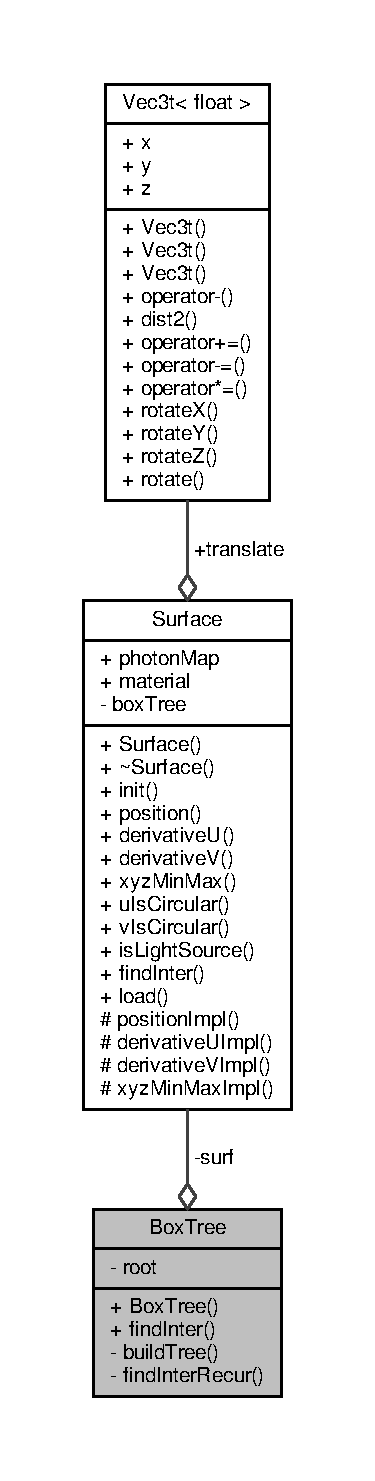
\includegraphics[height=550pt]{classBoxTree__coll__graph}
\end{center}
\end{figure}
\subsection*{Classes}
\begin{DoxyCompactItemize}
\item 
struct \hyperlink{structBoxTree_1_1Node}{Node}
\end{DoxyCompactItemize}
\subsection*{Public Member Functions}
\begin{DoxyCompactItemize}
\item 
\hyperlink{classBoxTree_a429e95ce51bc58ecd0e15eb11bac60dd}{Box\+Tree} (const \hyperlink{classSurface}{Surface} \&\+\_\+surf)
\item 
\hyperlink{classOptional}{Optional}$<$ \hyperlink{structSurfInterType}{Surf\+Inter\+Type} $>$ \hyperlink{classBoxTree_a3bfd0be9d94e7b6917a734b0474d8cff}{find\+Inter} (const \hyperlink{structRay}{Ray} \&ray) const 
\end{DoxyCompactItemize}
\subsection*{Private Member Functions}
\begin{DoxyCompactItemize}
\item 
void \hyperlink{classBoxTree_aff124ae5af1c4ecf8187a7473828229b}{build\+Tree} (const \hyperlink{classSurface}{Surface} \&\hyperlink{classBoxTree_a5c38df1ae1af50fa873ebde61b24df67}{surf}, std\+::unique\+\_\+ptr$<$ \hyperlink{structBoxTree_1_1Node}{Node} $>$ \&node, float u1, float u2, float v1, float v2)
\item 
\hyperlink{classOptional}{Optional}$<$ \hyperlink{structSurfInterType}{Surf\+Inter\+Type} $>$ \hyperlink{classBoxTree_a1ce4beeb452ab28f9927d00839f638fe}{find\+Inter\+Recur} (const \hyperlink{structRay}{Ray} \&ray, const std\+::unique\+\_\+ptr$<$ \hyperlink{structBoxTree_1_1Node}{Node} $>$ \&node, const \hyperlink{intersection_8h_a880ab27cdd7ea5eab91289bba0bacadb}{Inter\+Type} \&inter) const 
\begin{DoxyCompactList}\small\item\em Implement of find\+Inter Asserting ray is intersecting with node-\/$>$box. \end{DoxyCompactList}\end{DoxyCompactItemize}
\subsection*{Private Attributes}
\begin{DoxyCompactItemize}
\item 
std\+::unique\+\_\+ptr$<$ \hyperlink{structBoxTree_1_1Node}{Node} $>$ \hyperlink{classBoxTree_a12ff787723bc271b246f2662ce7c59b5}{root}
\item 
const \hyperlink{classSurface}{Surface} \& \hyperlink{classBoxTree_a5c38df1ae1af50fa873ebde61b24df67}{surf}
\end{DoxyCompactItemize}


\subsection{Detailed Description}
Tree of bounding box built on a surface Organized by surface parameters (u, v) 

\subsection{Constructor \& Destructor Documentation}
\index{Box\+Tree@{Box\+Tree}!Box\+Tree@{Box\+Tree}}
\index{Box\+Tree@{Box\+Tree}!Box\+Tree@{Box\+Tree}}
\subsubsection[{\texorpdfstring{Box\+Tree(const Surface \&\+\_\+surf)}{BoxTree(const Surface &_surf)}}]{\setlength{\rightskip}{0pt plus 5cm}Box\+Tree\+::\+Box\+Tree (
\begin{DoxyParamCaption}
\item[{const {\bf Surface} \&}]{\+\_\+surf}
\end{DoxyParamCaption}
)}\hypertarget{classBoxTree_a429e95ce51bc58ecd0e15eb11bac60dd}{}\label{classBoxTree_a429e95ce51bc58ecd0e15eb11bac60dd}


\subsection{Member Function Documentation}
\index{Box\+Tree@{Box\+Tree}!build\+Tree@{build\+Tree}}
\index{build\+Tree@{build\+Tree}!Box\+Tree@{Box\+Tree}}
\subsubsection[{\texorpdfstring{build\+Tree(const Surface \&surf, std\+::unique\+\_\+ptr$<$ Node $>$ \&node, float u1, float u2, float v1, float v2)}{buildTree(const Surface &surf, std::unique_ptr< Node > &node, float u1, float u2, float v1, float v2)}}]{\setlength{\rightskip}{0pt plus 5cm}void Box\+Tree\+::build\+Tree (
\begin{DoxyParamCaption}
\item[{const {\bf Surface} \&}]{surf, }
\item[{std\+::unique\+\_\+ptr$<$ {\bf Node} $>$ \&}]{node, }
\item[{float}]{u1, }
\item[{float}]{u2, }
\item[{float}]{v1, }
\item[{float}]{v2}
\end{DoxyParamCaption}
)\hspace{0.3cm}{\ttfamily [private]}}\hypertarget{classBoxTree_aff124ae5af1c4ecf8187a7473828229b}{}\label{classBoxTree_aff124ae5af1c4ecf8187a7473828229b}
\index{Box\+Tree@{Box\+Tree}!find\+Inter@{find\+Inter}}
\index{find\+Inter@{find\+Inter}!Box\+Tree@{Box\+Tree}}
\subsubsection[{\texorpdfstring{find\+Inter(const Ray \&ray) const }{findInter(const Ray &ray) const }}]{\setlength{\rightskip}{0pt plus 5cm}{\bf Optional}$<$ {\bf Surf\+Inter\+Type} $>$ Box\+Tree\+::find\+Inter (
\begin{DoxyParamCaption}
\item[{const {\bf Ray} \&}]{ray}
\end{DoxyParamCaption}
) const}\hypertarget{classBoxTree_a3bfd0be9d94e7b6917a734b0474d8cff}{}\label{classBoxTree_a3bfd0be9d94e7b6917a734b0474d8cff}
\index{Box\+Tree@{Box\+Tree}!find\+Inter\+Recur@{find\+Inter\+Recur}}
\index{find\+Inter\+Recur@{find\+Inter\+Recur}!Box\+Tree@{Box\+Tree}}
\subsubsection[{\texorpdfstring{find\+Inter\+Recur(const Ray \&ray, const std\+::unique\+\_\+ptr$<$ Node $>$ \&node, const Inter\+Type \&inter) const }{findInterRecur(const Ray &ray, const std::unique_ptr< Node > &node, const InterType &inter) const }}]{\setlength{\rightskip}{0pt plus 5cm}{\bf Optional}$<$ {\bf Surf\+Inter\+Type} $>$ Box\+Tree\+::find\+Inter\+Recur (
\begin{DoxyParamCaption}
\item[{const {\bf Ray} \&}]{ray, }
\item[{const std\+::unique\+\_\+ptr$<$ {\bf Node} $>$ \&}]{node, }
\item[{const {\bf Inter\+Type} \&}]{inter}
\end{DoxyParamCaption}
) const\hspace{0.3cm}{\ttfamily [private]}}\hypertarget{classBoxTree_a1ce4beeb452ab28f9927d00839f638fe}{}\label{classBoxTree_a1ce4beeb452ab28f9927d00839f638fe}


Implement of find\+Inter Asserting ray is intersecting with node-\/$>$box. 


\begin{DoxyParams}{Parameters}
{\em inter} & \+: intersecting point with \\
\hline
\end{DoxyParams}


\subsection{Member Data Documentation}
\index{Box\+Tree@{Box\+Tree}!root@{root}}
\index{root@{root}!Box\+Tree@{Box\+Tree}}
\subsubsection[{\texorpdfstring{root}{root}}]{\setlength{\rightskip}{0pt plus 5cm}std\+::unique\+\_\+ptr$<${\bf Node}$>$ Box\+Tree\+::root\hspace{0.3cm}{\ttfamily [private]}}\hypertarget{classBoxTree_a12ff787723bc271b246f2662ce7c59b5}{}\label{classBoxTree_a12ff787723bc271b246f2662ce7c59b5}
\index{Box\+Tree@{Box\+Tree}!surf@{surf}}
\index{surf@{surf}!Box\+Tree@{Box\+Tree}}
\subsubsection[{\texorpdfstring{surf}{surf}}]{\setlength{\rightskip}{0pt plus 5cm}const {\bf Surface}\& Box\+Tree\+::surf\hspace{0.3cm}{\ttfamily [private]}}\hypertarget{classBoxTree_a5c38df1ae1af50fa873ebde61b24df67}{}\label{classBoxTree_a5c38df1ae1af50fa873ebde61b24df67}


The documentation for this class was generated from the following files\+:\begin{DoxyCompactItemize}
\item 
\hyperlink{boxtree_8h}{boxtree.\+h}\item 
\hyperlink{boxtree_8cpp}{boxtree.\+cpp}\end{DoxyCompactItemize}

\hypertarget{structColoredRay}{}\section{Colored\+Ray Struct Reference}
\label{structColoredRay}\index{Colored\+Ray@{Colored\+Ray}}


{\ttfamily \#include $<$ray.\+h$>$}



Collaboration diagram for Colored\+Ray\+:\nopagebreak
\begin{figure}[H]
\begin{center}
\leavevmode
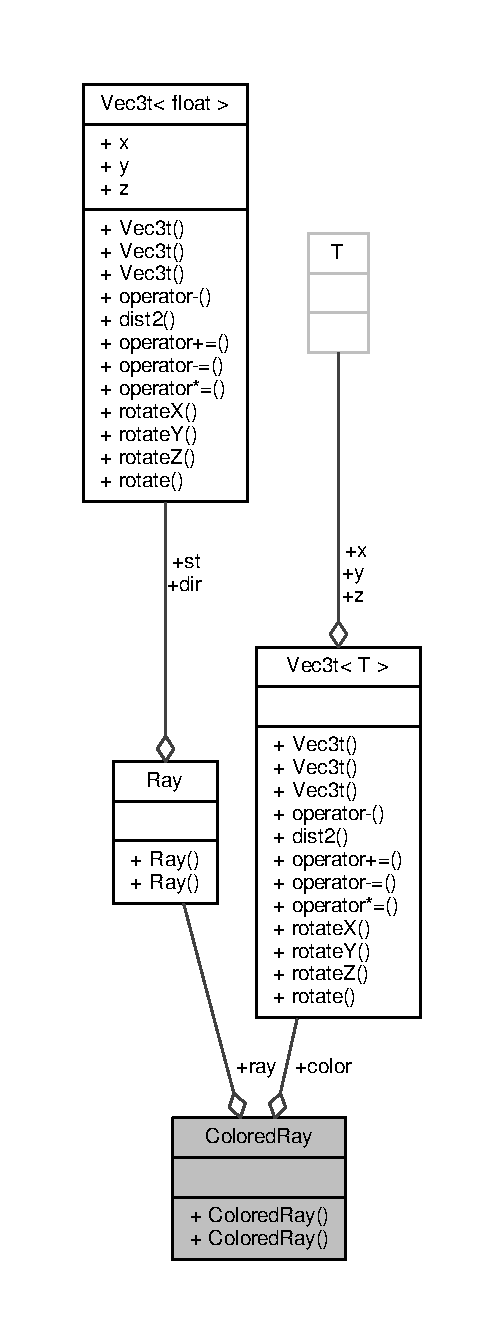
\includegraphics[height=550pt]{structColoredRay__coll__graph}
\end{center}
\end{figure}
\subsection*{Public Member Functions}
\begin{DoxyCompactItemize}
\item 
\hyperlink{structColoredRay_a3e9426d90cf6dce097cab957b55fc12f}{Colored\+Ray} ()
\item 
\hyperlink{structColoredRay_a4548637d5c8e89113f3f7b8332ade295}{Colored\+Ray} (const \hyperlink{ray_8h_a8a2580fb65f7d3d4e24bdd412b9bd92d}{color\+\_\+t} \&\+\_\+color, const \hyperlink{structRay}{Ray} \&\+\_\+ray)
\end{DoxyCompactItemize}
\subsection*{Public Attributes}
\begin{DoxyCompactItemize}
\item 
\hyperlink{ray_8h_a8a2580fb65f7d3d4e24bdd412b9bd92d}{color\+\_\+t} \hyperlink{structColoredRay_a25677d1a49f54e8ae35c09adc433c62a}{color}
\item 
\hyperlink{structRay}{Ray} \hyperlink{structColoredRay_a611f02566718c14e40376dc360b7b8ef}{ray}
\end{DoxyCompactItemize}


\subsection{Constructor \& Destructor Documentation}
\index{Colored\+Ray@{Colored\+Ray}!Colored\+Ray@{Colored\+Ray}}
\index{Colored\+Ray@{Colored\+Ray}!Colored\+Ray@{Colored\+Ray}}
\subsubsection[{\texorpdfstring{Colored\+Ray()}{ColoredRay()}}]{\setlength{\rightskip}{0pt plus 5cm}Colored\+Ray\+::\+Colored\+Ray (
\begin{DoxyParamCaption}
{}
\end{DoxyParamCaption}
)\hspace{0.3cm}{\ttfamily [inline]}}\hypertarget{structColoredRay_a3e9426d90cf6dce097cab957b55fc12f}{}\label{structColoredRay_a3e9426d90cf6dce097cab957b55fc12f}
\index{Colored\+Ray@{Colored\+Ray}!Colored\+Ray@{Colored\+Ray}}
\index{Colored\+Ray@{Colored\+Ray}!Colored\+Ray@{Colored\+Ray}}
\subsubsection[{\texorpdfstring{Colored\+Ray(const color\+\_\+t \&\+\_\+color, const Ray \&\+\_\+ray)}{ColoredRay(const color_t &_color, const Ray &_ray)}}]{\setlength{\rightskip}{0pt plus 5cm}Colored\+Ray\+::\+Colored\+Ray (
\begin{DoxyParamCaption}
\item[{const {\bf color\+\_\+t} \&}]{\+\_\+color, }
\item[{const {\bf Ray} \&}]{\+\_\+ray}
\end{DoxyParamCaption}
)\hspace{0.3cm}{\ttfamily [inline]}}\hypertarget{structColoredRay_a4548637d5c8e89113f3f7b8332ade295}{}\label{structColoredRay_a4548637d5c8e89113f3f7b8332ade295}


\subsection{Member Data Documentation}
\index{Colored\+Ray@{Colored\+Ray}!color@{color}}
\index{color@{color}!Colored\+Ray@{Colored\+Ray}}
\subsubsection[{\texorpdfstring{color}{color}}]{\setlength{\rightskip}{0pt plus 5cm}{\bf color\+\_\+t} Colored\+Ray\+::color}\hypertarget{structColoredRay_a25677d1a49f54e8ae35c09adc433c62a}{}\label{structColoredRay_a25677d1a49f54e8ae35c09adc433c62a}
\index{Colored\+Ray@{Colored\+Ray}!ray@{ray}}
\index{ray@{ray}!Colored\+Ray@{Colored\+Ray}}
\subsubsection[{\texorpdfstring{ray}{ray}}]{\setlength{\rightskip}{0pt plus 5cm}{\bf Ray} Colored\+Ray\+::ray}\hypertarget{structColoredRay_a611f02566718c14e40376dc360b7b8ef}{}\label{structColoredRay_a611f02566718c14e40376dc360b7b8ef}


The documentation for this struct was generated from the following file\+:\begin{DoxyCompactItemize}
\item 
\hyperlink{ray_8h}{ray.\+h}\end{DoxyCompactItemize}

\hypertarget{classCurve}{}\section{Curve Class Reference}
\label{classCurve}\index{Curve@{Curve}}


\hyperlink{classCurve}{Curve} base class \hyperlink{classCurve}{Curve} with parameter t in \mbox{[}0,1\mbox{]}.  




{\ttfamily \#include $<$curve.\+h$>$}



Inheritance diagram for Curve\+:\nopagebreak
\begin{figure}[H]
\begin{center}
\leavevmode
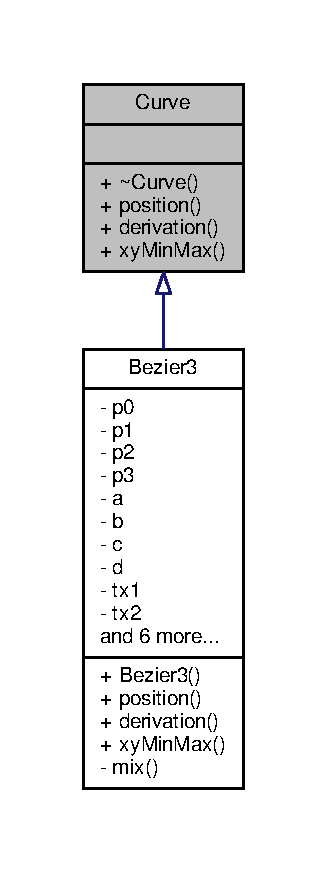
\includegraphics[width=157pt]{classCurve__inherit__graph}
\end{center}
\end{figure}


Collaboration diagram for Curve\+:\nopagebreak
\begin{figure}[H]
\begin{center}
\leavevmode
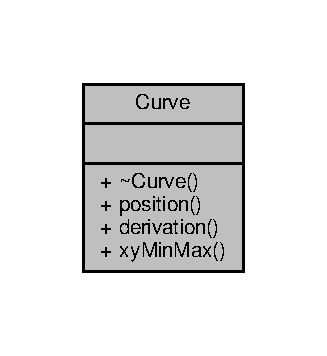
\includegraphics[width=157pt]{classCurve__coll__graph}
\end{center}
\end{figure}
\subsection*{Public Member Functions}
\begin{DoxyCompactItemize}
\item 
virtual \hyperlink{classCurve_ae7e4b9473d8b7d0b015eb0c230256498}{$\sim$\+Curve} ()
\item 
virtual \hyperlink{vec_8h_a871640c4eb6057d21b25824c55250629}{Vec2} \hyperlink{classCurve_a919ea6d17b6fc0dc6ea6facec6d5623c}{position} (float t) const =0
\begin{DoxyCompactList}\small\item\em Get point on the curve. \end{DoxyCompactList}\item 
virtual \hyperlink{vec_8h_a871640c4eb6057d21b25824c55250629}{Vec2} \hyperlink{classCurve_acca6db6f7d2f45fbea676db16e3784be}{derivation} (float t) const =0
\begin{DoxyCompactList}\small\item\em Get derivation. \end{DoxyCompactList}\item 
virtual \hyperlink{structBox2}{Box2} \hyperlink{classCurve_add48a303ee076bfce08340dd1241cbf6}{xy\+Min\+Max} (float t1, float t2) const =0
\begin{DoxyCompactList}\small\item\em (x\+:(min, max), y\+:(min, max)) when t in \mbox{[}x1, x2\mbox{]} \end{DoxyCompactList}\end{DoxyCompactItemize}


\subsection{Detailed Description}
\hyperlink{classCurve}{Curve} base class \hyperlink{classCurve}{Curve} with parameter t in \mbox{[}0,1\mbox{]}. 

\subsection{Constructor \& Destructor Documentation}
\index{Curve@{Curve}!````~Curve@{$\sim$\+Curve}}
\index{````~Curve@{$\sim$\+Curve}!Curve@{Curve}}
\subsubsection[{\texorpdfstring{$\sim$\+Curve()}{~Curve()}}]{\setlength{\rightskip}{0pt plus 5cm}virtual Curve\+::$\sim$\+Curve (
\begin{DoxyParamCaption}
{}
\end{DoxyParamCaption}
)\hspace{0.3cm}{\ttfamily [inline]}, {\ttfamily [virtual]}}\hypertarget{classCurve_ae7e4b9473d8b7d0b015eb0c230256498}{}\label{classCurve_ae7e4b9473d8b7d0b015eb0c230256498}


\subsection{Member Function Documentation}
\index{Curve@{Curve}!derivation@{derivation}}
\index{derivation@{derivation}!Curve@{Curve}}
\subsubsection[{\texorpdfstring{derivation(float t) const =0}{derivation(float t) const =0}}]{\setlength{\rightskip}{0pt plus 5cm}virtual {\bf Vec2} Curve\+::derivation (
\begin{DoxyParamCaption}
\item[{float}]{t}
\end{DoxyParamCaption}
) const\hspace{0.3cm}{\ttfamily [pure virtual]}}\hypertarget{classCurve_acca6db6f7d2f45fbea676db16e3784be}{}\label{classCurve_acca6db6f7d2f45fbea676db16e3784be}


Get derivation. 



Implemented in \hyperlink{classBezier3_a8f3bc3ba14dae6e9f27366ef587accc5}{Bezier3}.

\index{Curve@{Curve}!position@{position}}
\index{position@{position}!Curve@{Curve}}
\subsubsection[{\texorpdfstring{position(float t) const =0}{position(float t) const =0}}]{\setlength{\rightskip}{0pt plus 5cm}virtual {\bf Vec2} Curve\+::position (
\begin{DoxyParamCaption}
\item[{float}]{t}
\end{DoxyParamCaption}
) const\hspace{0.3cm}{\ttfamily [pure virtual]}}\hypertarget{classCurve_a919ea6d17b6fc0dc6ea6facec6d5623c}{}\label{classCurve_a919ea6d17b6fc0dc6ea6facec6d5623c}


Get point on the curve. 



Implemented in \hyperlink{classBezier3_afd1907f62d8d19b4683f43080a0334db}{Bezier3}.

\index{Curve@{Curve}!xy\+Min\+Max@{xy\+Min\+Max}}
\index{xy\+Min\+Max@{xy\+Min\+Max}!Curve@{Curve}}
\subsubsection[{\texorpdfstring{xy\+Min\+Max(float t1, float t2) const =0}{xyMinMax(float t1, float t2) const =0}}]{\setlength{\rightskip}{0pt plus 5cm}virtual {\bf Box2} Curve\+::xy\+Min\+Max (
\begin{DoxyParamCaption}
\item[{float}]{t1, }
\item[{float}]{t2}
\end{DoxyParamCaption}
) const\hspace{0.3cm}{\ttfamily [pure virtual]}}\hypertarget{classCurve_add48a303ee076bfce08340dd1241cbf6}{}\label{classCurve_add48a303ee076bfce08340dd1241cbf6}


(x\+:(min, max), y\+:(min, max)) when t in \mbox{[}x1, x2\mbox{]} 



Implemented in \hyperlink{classBezier3_aa5a1d33483071204f99774fefb092caf}{Bezier3}.



The documentation for this class was generated from the following file\+:\begin{DoxyCompactItemize}
\item 
\hyperlink{curve_8h}{curve.\+h}\end{DoxyCompactItemize}

\hypertarget{classKDTree}{}\section{K\+D\+Tree Class Reference}
\label{classKDTree}\index{K\+D\+Tree@{K\+D\+Tree}}


{\ttfamily \#include $<$kdtree.\+h$>$}



Collaboration diagram for K\+D\+Tree\+:
\nopagebreak
\begin{figure}[H]
\begin{center}
\leavevmode
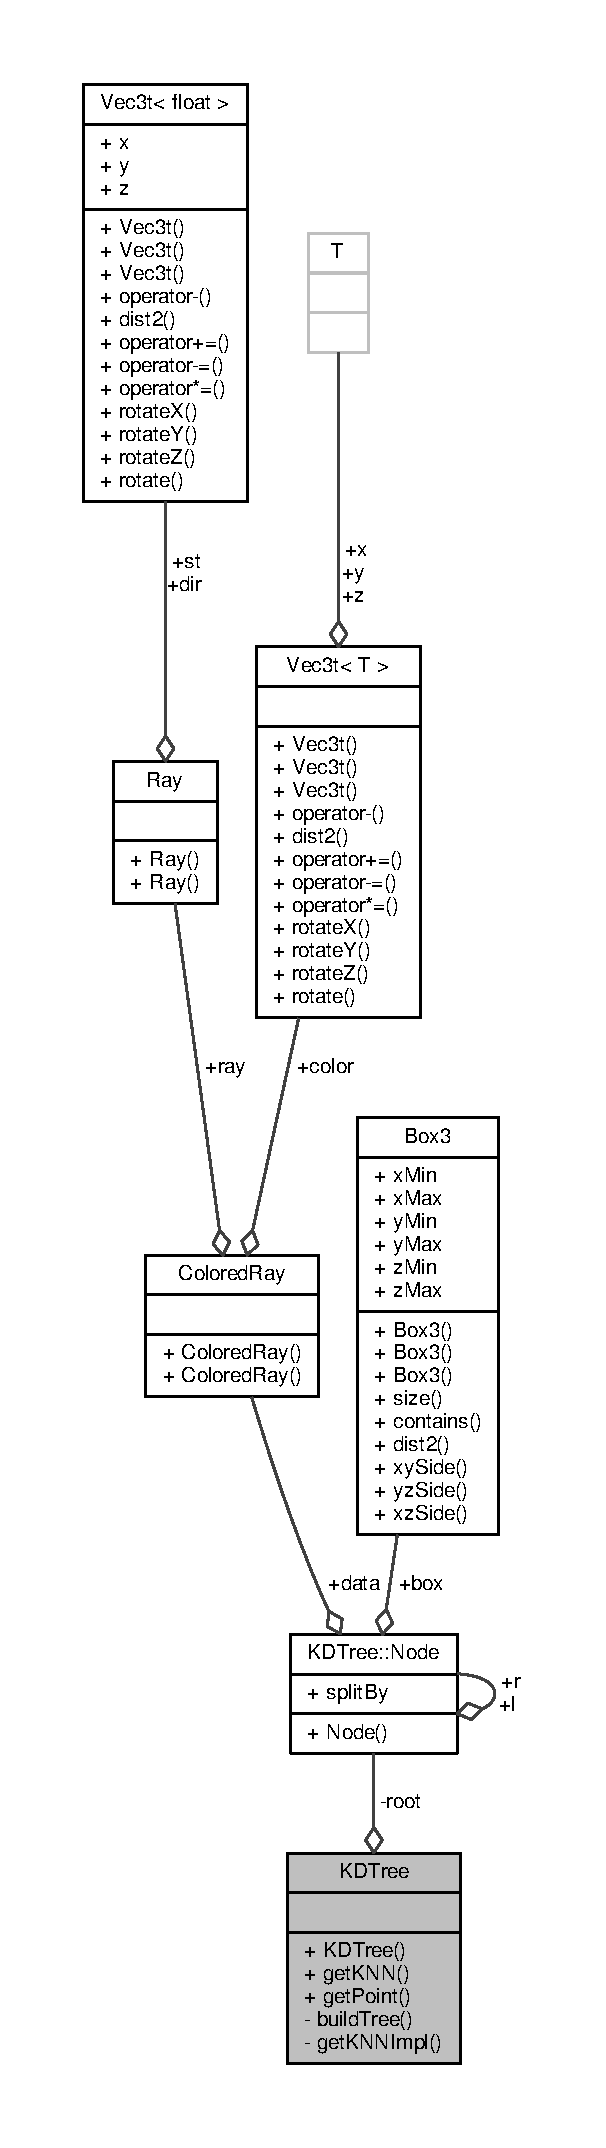
\includegraphics[height=550pt]{classKDTree__coll__graph}
\end{center}
\end{figure}
\subsection*{Classes}
\begin{DoxyCompactItemize}
\item 
struct \hyperlink{structKDTree_1_1Node}{Node}
\end{DoxyCompactItemize}
\subsection*{Public Types}
\begin{DoxyCompactItemize}
\item 
typedef \hyperlink{structColoredRay}{Colored\+Ray} \hyperlink{classKDTree_ab000d86d0fb4aaedcc83b5b7a584c25e}{data\+\_\+t}
\end{DoxyCompactItemize}
\subsection*{Public Member Functions}
\begin{DoxyCompactItemize}
\item 
\hyperlink{classKDTree_a4c0f47702f2326bef96eac59184502b4}{K\+D\+Tree} (std\+::vector$<$ \hyperlink{classKDTree_ab000d86d0fb4aaedcc83b5b7a584c25e}{data\+\_\+t} $>$ \&data)
\item 
std\+::vector$<$ \hyperlink{classKDTree_ab000d86d0fb4aaedcc83b5b7a584c25e}{data\+\_\+t} $>$ \hyperlink{classKDTree_af77f46cd77a1a798cf911a521563d3b3}{get\+K\+NN} (const \hyperlink{vec_8h_ae4fcaa7c0a3935930ed1be5f70b90373}{Vec3} \&center, int k) const 
\begin{DoxyCompactList}\small\item\em find {\ttfamily k} nearest neighbors around {\ttfamily center} \end{DoxyCompactList}\end{DoxyCompactItemize}
\subsection*{Static Public Member Functions}
\begin{DoxyCompactItemize}
\item 
static const \hyperlink{vec_8h_ae4fcaa7c0a3935930ed1be5f70b90373}{Vec3} \& \hyperlink{classKDTree_a40fd2a926b4d28ec387372553c51749b}{get\+Point} (const \hyperlink{classKDTree_ab000d86d0fb4aaedcc83b5b7a584c25e}{data\+\_\+t} \&data)
\begin{DoxyCompactList}\small\item\em {\ttfamily data} will be modified \end{DoxyCompactList}\end{DoxyCompactItemize}
\subsection*{Private Member Functions}
\begin{DoxyCompactItemize}
\item 
void \hyperlink{classKDTree_a4862664dcb6ac6ddc21a5447721ebab7}{build\+Tree} (std\+::vector$<$ \hyperlink{classKDTree_ab000d86d0fb4aaedcc83b5b7a584c25e}{data\+\_\+t} $>$ \&data, int l, int r, \hyperlink{structKDTree_1_1Node}{Node} $\ast$\&x, \hyperlink{structKDTree_1_1Node_ab21ae38de8fe0e25d29d0ae136a1db34}{Node\+::split\+\_\+t} split\+By)
\begin{DoxyCompactList}\small\item\em Build tree recursively. \end{DoxyCompactList}\item 
void \hyperlink{classKDTree_a5fed302ab0121b6903d60d1ae46a7654}{get\+K\+N\+N\+Impl} (const \hyperlink{structKDTree_1_1Node}{Node} $\ast$x, std\+::vector$<$ \hyperlink{classKDTree_ab000d86d0fb4aaedcc83b5b7a584c25e}{data\+\_\+t} $>$ \&res, const \hyperlink{vec_8h_ae4fcaa7c0a3935930ed1be5f70b90373}{Vec3} \&center, int k) const 
\begin{DoxyCompactList}\small\item\em Get K\+NN recursively. \end{DoxyCompactList}\end{DoxyCompactItemize}
\subsection*{Private Attributes}
\begin{DoxyCompactItemize}
\item 
struct \hyperlink{structKDTree_1_1Node}{K\+D\+Tree\+::\+Node} $\ast$ \hyperlink{classKDTree_af6c514e842e138504160e8d14fa084f7}{root}
\end{DoxyCompactItemize}


\subsection{Member Typedef Documentation}
\index{K\+D\+Tree@{K\+D\+Tree}!data\+\_\+t@{data\+\_\+t}}
\index{data\+\_\+t@{data\+\_\+t}!K\+D\+Tree@{K\+D\+Tree}}
\subsubsection[{\texorpdfstring{data\+\_\+t}{data_t}}]{\setlength{\rightskip}{0pt plus 5cm}typedef {\bf Colored\+Ray} {\bf K\+D\+Tree\+::data\+\_\+t}}\hypertarget{classKDTree_ab000d86d0fb4aaedcc83b5b7a584c25e}{}\label{classKDTree_ab000d86d0fb4aaedcc83b5b7a584c25e}


\subsection{Constructor \& Destructor Documentation}
\index{K\+D\+Tree@{K\+D\+Tree}!K\+D\+Tree@{K\+D\+Tree}}
\index{K\+D\+Tree@{K\+D\+Tree}!K\+D\+Tree@{K\+D\+Tree}}
\subsubsection[{\texorpdfstring{K\+D\+Tree(std\+::vector$<$ data\+\_\+t $>$ \&data)}{KDTree(std::vector< data_t > &data)}}]{\setlength{\rightskip}{0pt plus 5cm}K\+D\+Tree\+::\+K\+D\+Tree (
\begin{DoxyParamCaption}
\item[{std\+::vector$<$ {\bf data\+\_\+t} $>$ \&}]{data}
\end{DoxyParamCaption}
)\hspace{0.3cm}{\ttfamily [inline]}}\hypertarget{classKDTree_a4c0f47702f2326bef96eac59184502b4}{}\label{classKDTree_a4c0f47702f2326bef96eac59184502b4}


\subsection{Member Function Documentation}
\index{K\+D\+Tree@{K\+D\+Tree}!build\+Tree@{build\+Tree}}
\index{build\+Tree@{build\+Tree}!K\+D\+Tree@{K\+D\+Tree}}
\subsubsection[{\texorpdfstring{build\+Tree(std\+::vector$<$ data\+\_\+t $>$ \&data, int l, int r, Node $\ast$\&x, Node\+::split\+\_\+t split\+By)}{buildTree(std::vector< data_t > &data, int l, int r, Node *&x, Node::split_t splitBy)}}]{\setlength{\rightskip}{0pt plus 5cm}void K\+D\+Tree\+::build\+Tree (
\begin{DoxyParamCaption}
\item[{std\+::vector$<$ {\bf data\+\_\+t} $>$ \&}]{data, }
\item[{int}]{l, }
\item[{int}]{r, }
\item[{{\bf Node} $\ast$\&}]{x, }
\item[{{\bf Node\+::split\+\_\+t}}]{split\+By}
\end{DoxyParamCaption}
)\hspace{0.3cm}{\ttfamily [private]}}\hypertarget{classKDTree_a4862664dcb6ac6ddc21a5447721ebab7}{}\label{classKDTree_a4862664dcb6ac6ddc21a5447721ebab7}


Build tree recursively. 


\begin{DoxyParams}{Parameters}
{\em data} & \+: All points built into K\+D-\/tree. Will be modified \\
\hline
{\em l,r,x} & \+: Current node is {\ttfamily x} which represent range \mbox{[}l, r) \\
\hline
{\em split\+By} & \+: Splitting direction. This is cycling \\
\hline
\end{DoxyParams}
\index{K\+D\+Tree@{K\+D\+Tree}!get\+K\+NN@{get\+K\+NN}}
\index{get\+K\+NN@{get\+K\+NN}!K\+D\+Tree@{K\+D\+Tree}}
\subsubsection[{\texorpdfstring{get\+K\+N\+N(const Vec3 \&center, int k) const }{getKNN(const Vec3 &center, int k) const }}]{\setlength{\rightskip}{0pt plus 5cm}std\+::vector$<$ {\bf K\+D\+Tree\+::data\+\_\+t} $>$ K\+D\+Tree\+::get\+K\+NN (
\begin{DoxyParamCaption}
\item[{const {\bf Vec3} \&}]{center, }
\item[{int}]{k}
\end{DoxyParamCaption}
) const\hspace{0.3cm}{\ttfamily [inline]}}\hypertarget{classKDTree_af77f46cd77a1a798cf911a521563d3b3}{}\label{classKDTree_af77f46cd77a1a798cf911a521563d3b3}


find {\ttfamily k} nearest neighbors around {\ttfamily center} 

\index{K\+D\+Tree@{K\+D\+Tree}!get\+K\+N\+N\+Impl@{get\+K\+N\+N\+Impl}}
\index{get\+K\+N\+N\+Impl@{get\+K\+N\+N\+Impl}!K\+D\+Tree@{K\+D\+Tree}}
\subsubsection[{\texorpdfstring{get\+K\+N\+N\+Impl(const Node $\ast$x, std\+::vector$<$ data\+\_\+t $>$ \&res, const Vec3 \&center, int k) const }{getKNNImpl(const Node *x, std::vector< data_t > &res, const Vec3 &center, int k) const }}]{\setlength{\rightskip}{0pt plus 5cm}void K\+D\+Tree\+::get\+K\+N\+N\+Impl (
\begin{DoxyParamCaption}
\item[{const {\bf Node} $\ast$}]{x, }
\item[{std\+::vector$<$ {\bf data\+\_\+t} $>$ \&}]{res, }
\item[{const {\bf Vec3} \&}]{center, }
\item[{int}]{k}
\end{DoxyParamCaption}
) const\hspace{0.3cm}{\ttfamily [private]}}\hypertarget{classKDTree_a5fed302ab0121b6903d60d1ae46a7654}{}\label{classKDTree_a5fed302ab0121b6903d60d1ae46a7654}


Get K\+NN recursively. 


\begin{DoxyParams}{Parameters}
{\em x} & \+: Current node \\
\hline
{\em res} & \+: Results \\
\hline
{\em center,k} & \+: See get\+K\+NN \\
\hline
\end{DoxyParams}
\index{K\+D\+Tree@{K\+D\+Tree}!get\+Point@{get\+Point}}
\index{get\+Point@{get\+Point}!K\+D\+Tree@{K\+D\+Tree}}
\subsubsection[{\texorpdfstring{get\+Point(const data\+\_\+t \&data)}{getPoint(const data_t &data)}}]{\setlength{\rightskip}{0pt plus 5cm}const {\bf Vec3} \& K\+D\+Tree\+::get\+Point (
\begin{DoxyParamCaption}
\item[{const {\bf data\+\_\+t} \&}]{data}
\end{DoxyParamCaption}
)\hspace{0.3cm}{\ttfamily [inline]}, {\ttfamily [static]}}\hypertarget{classKDTree_a40fd2a926b4d28ec387372553c51749b}{}\label{classKDTree_a40fd2a926b4d28ec387372553c51749b}


{\ttfamily data} will be modified 

Get point that used in this kd-\/tree from data\+\_\+t 

\subsection{Member Data Documentation}
\index{K\+D\+Tree@{K\+D\+Tree}!root@{root}}
\index{root@{root}!K\+D\+Tree@{K\+D\+Tree}}
\subsubsection[{\texorpdfstring{root}{root}}]{\setlength{\rightskip}{0pt plus 5cm}struct {\bf K\+D\+Tree\+::\+Node} $\ast$ K\+D\+Tree\+::root\hspace{0.3cm}{\ttfamily [private]}}\hypertarget{classKDTree_af6c514e842e138504160e8d14fa084f7}{}\label{classKDTree_af6c514e842e138504160e8d14fa084f7}


The documentation for this class was generated from the following files\+:\begin{DoxyCompactItemize}
\item 
\hyperlink{kdtree_8h}{kdtree.\+h}\item 
\hyperlink{kdtree_8cpp}{kdtree.\+cpp}\end{DoxyCompactItemize}

\hypertarget{classLightSource}{}\section{Light\+Source Class Reference}
\label{classLightSource}\index{Light\+Source@{Light\+Source}}


Light source as a ball Cannot be used as a normal object.  




{\ttfamily \#include $<$lightsource.\+h$>$}



Inheritance diagram for Light\+Source\+:
\nopagebreak
\begin{figure}[H]
\begin{center}
\leavevmode
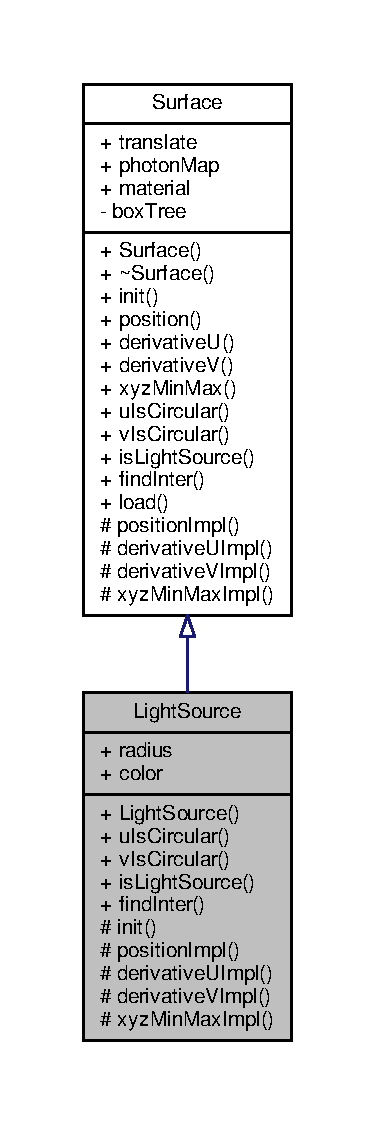
\includegraphics[width=180pt]{classLightSource__inherit__graph}
\end{center}
\end{figure}


Collaboration diagram for Light\+Source\+:
\nopagebreak
\begin{figure}[H]
\begin{center}
\leavevmode
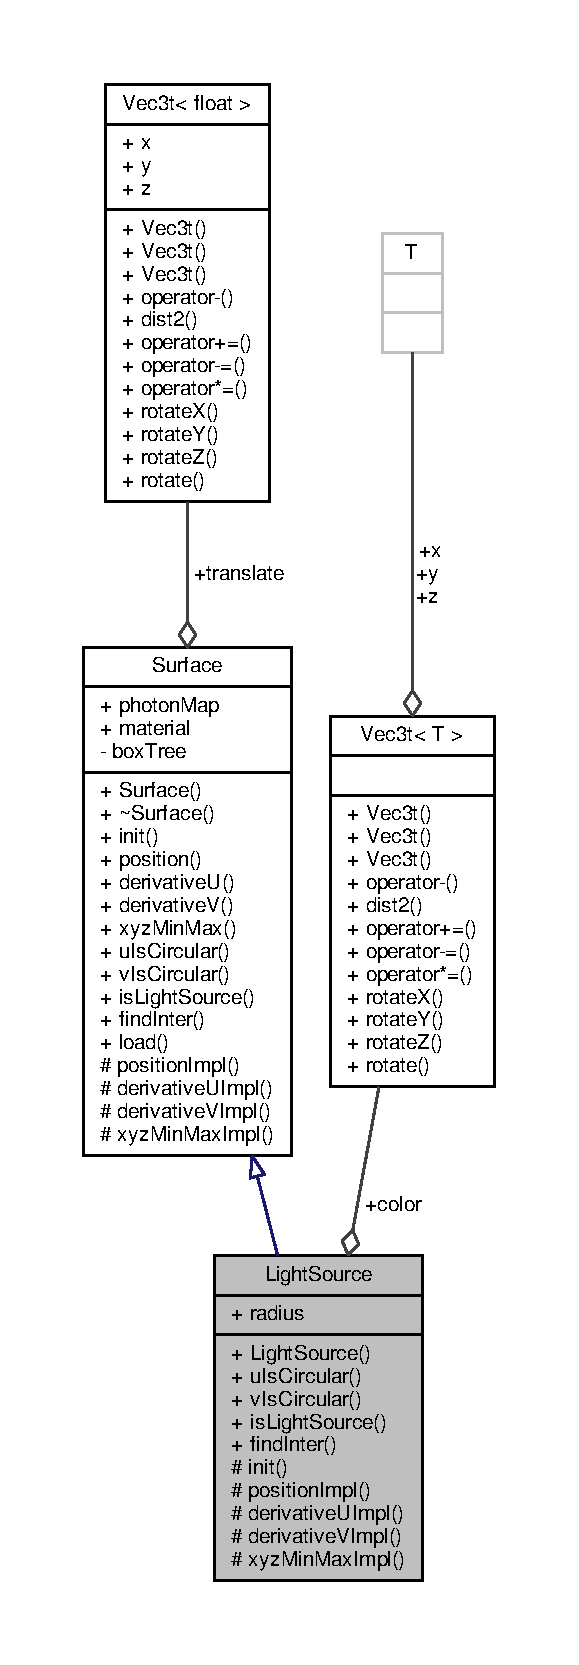
\includegraphics[height=550pt]{classLightSource__coll__graph}
\end{center}
\end{figure}
\subsection*{Public Member Functions}
\begin{DoxyCompactItemize}
\item 
\hyperlink{classLightSource_a9ab7d1b421af490fe5c684e00dae44bc}{Light\+Source} (float \+\_\+radius, const \hyperlink{ray_8h_a8a2580fb65f7d3d4e24bdd412b9bd92d}{color\+\_\+t} \&\+\_\+color)
\item 
bool \hyperlink{classLightSource_a6d1e29c394c2ae29c6b913376a3ebbc5}{u\+Is\+Circular} () const override
\item 
bool \hyperlink{classLightSource_a617519569f55a575189f0de58f0b8a11}{v\+Is\+Circular} () const override
\item 
bool \hyperlink{classLightSource_a5d397dd1719c8aaf9d711bace27a9547}{is\+Light\+Source} () const override
\item 
\hyperlink{classOptional}{Optional}$<$ \hyperlink{structSurfInterType}{Surf\+Inter\+Type} $>$ \hyperlink{classLightSource_a7470bd637b7013e310c1a6789d12de92}{find\+Inter} (const \hyperlink{structRay}{Ray} \&ray) const override
\begin{DoxyCompactList}\small\item\em This function is can only returns t and pos. \end{DoxyCompactList}\end{DoxyCompactItemize}
\subsection*{Public Attributes}
\begin{DoxyCompactItemize}
\item 
float \hyperlink{classLightSource_a6dbf2113c6dac64e323ebf4f691d1e66}{radius}
\item 
\hyperlink{ray_8h_a8a2580fb65f7d3d4e24bdd412b9bd92d}{color\+\_\+t} \hyperlink{classLightSource_a4a567c627c51e5850af199a8af6bea27}{color}
\end{DoxyCompactItemize}
\subsection*{Protected Member Functions}
\begin{DoxyCompactItemize}
\item 
void \hyperlink{classLightSource_a9001c11824ce30f44bdd9a729cc420a6}{init} () override
\begin{DoxyCompactList}\small\item\em Something can\textquotesingle{}t be put in constructor. \end{DoxyCompactList}\item 
\hyperlink{vec_8h_ae4fcaa7c0a3935930ed1be5f70b90373}{Vec3} \hyperlink{classLightSource_a1ac118f57425ed163c6ab45d6320f401}{position\+Impl} (float u, float v) const override
\begin{DoxyCompactList}\small\item\em Do nothing because find\+Inter is overrided. \end{DoxyCompactList}\item 
\hyperlink{vec_8h_ae4fcaa7c0a3935930ed1be5f70b90373}{Vec3} \hyperlink{classLightSource_ac9506b1c3f773b0de0c30ca78b4a9aa0}{derivative\+U\+Impl} (float u, float v) const override
\begin{DoxyCompactList}\small\item\em Forbidden. \end{DoxyCompactList}\item 
\hyperlink{vec_8h_ae4fcaa7c0a3935930ed1be5f70b90373}{Vec3} \hyperlink{classLightSource_a90b1596aca4c3b818fe73d8ef35065da}{derivative\+V\+Impl} (float u, float v) const override
\item 
\hyperlink{structBox3}{Box3} \hyperlink{classLightSource_a01f7d7c1cca3b8ab7ec688253a46aaec}{xyz\+Min\+Max\+Impl} (float u1, float u2, float v1, float v2) const override
\end{DoxyCompactItemize}
\subsection*{Additional Inherited Members}


\subsection{Detailed Description}
Light source as a ball Cannot be used as a normal object. 

\subsection{Constructor \& Destructor Documentation}
\index{Light\+Source@{Light\+Source}!Light\+Source@{Light\+Source}}
\index{Light\+Source@{Light\+Source}!Light\+Source@{Light\+Source}}
\subsubsection[{\texorpdfstring{Light\+Source(float \+\_\+radius, const color\+\_\+t \&\+\_\+color)}{LightSource(float _radius, const color_t &_color)}}]{\setlength{\rightskip}{0pt plus 5cm}Light\+Source\+::\+Light\+Source (
\begin{DoxyParamCaption}
\item[{float}]{\+\_\+radius, }
\item[{const {\bf color\+\_\+t} \&}]{\+\_\+color}
\end{DoxyParamCaption}
)\hspace{0.3cm}{\ttfamily [inline]}}\hypertarget{classLightSource_a9ab7d1b421af490fe5c684e00dae44bc}{}\label{classLightSource_a9ab7d1b421af490fe5c684e00dae44bc}


\subsection{Member Function Documentation}
\index{Light\+Source@{Light\+Source}!derivative\+U\+Impl@{derivative\+U\+Impl}}
\index{derivative\+U\+Impl@{derivative\+U\+Impl}!Light\+Source@{Light\+Source}}
\subsubsection[{\texorpdfstring{derivative\+U\+Impl(float u, float v) const override}{derivativeUImpl(float u, float v) const override}}]{\setlength{\rightskip}{0pt plus 5cm}{\bf Vec3} Light\+Source\+::derivative\+U\+Impl (
\begin{DoxyParamCaption}
\item[{float}]{u, }
\item[{float}]{v}
\end{DoxyParamCaption}
) const\hspace{0.3cm}{\ttfamily [inline]}, {\ttfamily [override]}, {\ttfamily [protected]}, {\ttfamily [virtual]}}\hypertarget{classLightSource_ac9506b1c3f773b0de0c30ca78b4a9aa0}{}\label{classLightSource_ac9506b1c3f773b0de0c30ca78b4a9aa0}


Forbidden. 



Implements \hyperlink{classSurface_a4de8fb9d4652cc32022c95eb903cce4a}{Surface}.

\index{Light\+Source@{Light\+Source}!derivative\+V\+Impl@{derivative\+V\+Impl}}
\index{derivative\+V\+Impl@{derivative\+V\+Impl}!Light\+Source@{Light\+Source}}
\subsubsection[{\texorpdfstring{derivative\+V\+Impl(float u, float v) const override}{derivativeVImpl(float u, float v) const override}}]{\setlength{\rightskip}{0pt plus 5cm}{\bf Vec3} Light\+Source\+::derivative\+V\+Impl (
\begin{DoxyParamCaption}
\item[{float}]{u, }
\item[{float}]{v}
\end{DoxyParamCaption}
) const\hspace{0.3cm}{\ttfamily [inline]}, {\ttfamily [override]}, {\ttfamily [protected]}, {\ttfamily [virtual]}}\hypertarget{classLightSource_a90b1596aca4c3b818fe73d8ef35065da}{}\label{classLightSource_a90b1596aca4c3b818fe73d8ef35065da}


Implements \hyperlink{classSurface_a95d65437419ba8d439fa8f0d71f963a1}{Surface}.

\index{Light\+Source@{Light\+Source}!find\+Inter@{find\+Inter}}
\index{find\+Inter@{find\+Inter}!Light\+Source@{Light\+Source}}
\subsubsection[{\texorpdfstring{find\+Inter(const Ray \&ray) const override}{findInter(const Ray &ray) const override}}]{\setlength{\rightskip}{0pt plus 5cm}{\bf Optional}$<$ {\bf Surf\+Inter\+Type} $>$ Light\+Source\+::find\+Inter (
\begin{DoxyParamCaption}
\item[{const {\bf Ray} \&}]{ray}
\end{DoxyParamCaption}
) const\hspace{0.3cm}{\ttfamily [inline]}, {\ttfamily [override]}, {\ttfamily [virtual]}}\hypertarget{classLightSource_a7470bd637b7013e310c1a6789d12de92}{}\label{classLightSource_a7470bd637b7013e310c1a6789d12de92}


This function is can only returns t and pos. 



Reimplemented from \hyperlink{classSurface_af7b5584007bf626bf7b37fcf649e6cd6}{Surface}.

\index{Light\+Source@{Light\+Source}!init@{init}}
\index{init@{init}!Light\+Source@{Light\+Source}}
\subsubsection[{\texorpdfstring{init() override}{init() override}}]{\setlength{\rightskip}{0pt plus 5cm}void Light\+Source\+::init (
\begin{DoxyParamCaption}
{}
\end{DoxyParamCaption}
)\hspace{0.3cm}{\ttfamily [inline]}, {\ttfamily [override]}, {\ttfamily [protected]}, {\ttfamily [virtual]}}\hypertarget{classLightSource_a9001c11824ce30f44bdd9a729cc420a6}{}\label{classLightSource_a9001c11824ce30f44bdd9a729cc420a6}


Something can\textquotesingle{}t be put in constructor. 



Reimplemented from \hyperlink{classSurface_a194087202684a4b3a71c24f02faeb404}{Surface}.

\index{Light\+Source@{Light\+Source}!is\+Light\+Source@{is\+Light\+Source}}
\index{is\+Light\+Source@{is\+Light\+Source}!Light\+Source@{Light\+Source}}
\subsubsection[{\texorpdfstring{is\+Light\+Source() const override}{isLightSource() const override}}]{\setlength{\rightskip}{0pt plus 5cm}bool Light\+Source\+::is\+Light\+Source (
\begin{DoxyParamCaption}
{}
\end{DoxyParamCaption}
) const\hspace{0.3cm}{\ttfamily [inline]}, {\ttfamily [override]}, {\ttfamily [virtual]}}\hypertarget{classLightSource_a5d397dd1719c8aaf9d711bace27a9547}{}\label{classLightSource_a5d397dd1719c8aaf9d711bace27a9547}


Reimplemented from \hyperlink{classSurface_a5968cee515dd97f1e5066fec7cbf9b03}{Surface}.

\index{Light\+Source@{Light\+Source}!position\+Impl@{position\+Impl}}
\index{position\+Impl@{position\+Impl}!Light\+Source@{Light\+Source}}
\subsubsection[{\texorpdfstring{position\+Impl(float u, float v) const override}{positionImpl(float u, float v) const override}}]{\setlength{\rightskip}{0pt plus 5cm}{\bf Vec3} Light\+Source\+::position\+Impl (
\begin{DoxyParamCaption}
\item[{float}]{u, }
\item[{float}]{v}
\end{DoxyParamCaption}
) const\hspace{0.3cm}{\ttfamily [inline]}, {\ttfamily [override]}, {\ttfamily [protected]}, {\ttfamily [virtual]}}\hypertarget{classLightSource_a1ac118f57425ed163c6ab45d6320f401}{}\label{classLightSource_a1ac118f57425ed163c6ab45d6320f401}


Do nothing because find\+Inter is overrided. 



Implements \hyperlink{classSurface_a379545eea4809f81fe7e037f5e5ff4be}{Surface}.

\index{Light\+Source@{Light\+Source}!u\+Is\+Circular@{u\+Is\+Circular}}
\index{u\+Is\+Circular@{u\+Is\+Circular}!Light\+Source@{Light\+Source}}
\subsubsection[{\texorpdfstring{u\+Is\+Circular() const override}{uIsCircular() const override}}]{\setlength{\rightskip}{0pt plus 5cm}bool Light\+Source\+::u\+Is\+Circular (
\begin{DoxyParamCaption}
{}
\end{DoxyParamCaption}
) const\hspace{0.3cm}{\ttfamily [inline]}, {\ttfamily [override]}, {\ttfamily [virtual]}}\hypertarget{classLightSource_a6d1e29c394c2ae29c6b913376a3ebbc5}{}\label{classLightSource_a6d1e29c394c2ae29c6b913376a3ebbc5}


Implements \hyperlink{classSurface_a11d5759ec3e3d43036fb949dcc6f5562}{Surface}.

\index{Light\+Source@{Light\+Source}!v\+Is\+Circular@{v\+Is\+Circular}}
\index{v\+Is\+Circular@{v\+Is\+Circular}!Light\+Source@{Light\+Source}}
\subsubsection[{\texorpdfstring{v\+Is\+Circular() const override}{vIsCircular() const override}}]{\setlength{\rightskip}{0pt plus 5cm}bool Light\+Source\+::v\+Is\+Circular (
\begin{DoxyParamCaption}
{}
\end{DoxyParamCaption}
) const\hspace{0.3cm}{\ttfamily [inline]}, {\ttfamily [override]}, {\ttfamily [virtual]}}\hypertarget{classLightSource_a617519569f55a575189f0de58f0b8a11}{}\label{classLightSource_a617519569f55a575189f0de58f0b8a11}


Implements \hyperlink{classSurface_af52f9322929a702a9aaeee3ae4a368da}{Surface}.

\index{Light\+Source@{Light\+Source}!xyz\+Min\+Max\+Impl@{xyz\+Min\+Max\+Impl}}
\index{xyz\+Min\+Max\+Impl@{xyz\+Min\+Max\+Impl}!Light\+Source@{Light\+Source}}
\subsubsection[{\texorpdfstring{xyz\+Min\+Max\+Impl(float u1, float u2, float v1, float v2) const override}{xyzMinMaxImpl(float u1, float u2, float v1, float v2) const override}}]{\setlength{\rightskip}{0pt plus 5cm}{\bf Box3} Light\+Source\+::xyz\+Min\+Max\+Impl (
\begin{DoxyParamCaption}
\item[{float}]{u1, }
\item[{float}]{u2, }
\item[{float}]{v1, }
\item[{float}]{v2}
\end{DoxyParamCaption}
) const\hspace{0.3cm}{\ttfamily [inline]}, {\ttfamily [override]}, {\ttfamily [protected]}, {\ttfamily [virtual]}}\hypertarget{classLightSource_a01f7d7c1cca3b8ab7ec688253a46aaec}{}\label{classLightSource_a01f7d7c1cca3b8ab7ec688253a46aaec}


Implements \hyperlink{classSurface_ab1ee990da290748cd86aaf95edb28c38}{Surface}.



\subsection{Member Data Documentation}
\index{Light\+Source@{Light\+Source}!color@{color}}
\index{color@{color}!Light\+Source@{Light\+Source}}
\subsubsection[{\texorpdfstring{color}{color}}]{\setlength{\rightskip}{0pt plus 5cm}{\bf color\+\_\+t} Light\+Source\+::color}\hypertarget{classLightSource_a4a567c627c51e5850af199a8af6bea27}{}\label{classLightSource_a4a567c627c51e5850af199a8af6bea27}
\index{Light\+Source@{Light\+Source}!radius@{radius}}
\index{radius@{radius}!Light\+Source@{Light\+Source}}
\subsubsection[{\texorpdfstring{radius}{radius}}]{\setlength{\rightskip}{0pt plus 5cm}float Light\+Source\+::radius}\hypertarget{classLightSource_a6dbf2113c6dac64e323ebf4f691d1e66}{}\label{classLightSource_a6dbf2113c6dac64e323ebf4f691d1e66}


The documentation for this class was generated from the following file\+:\begin{DoxyCompactItemize}
\item 
\hyperlink{lightsource_8h}{lightsource.\+h}\end{DoxyCompactItemize}

\hypertarget{structMaterial}{}\section{Material Struct Reference}
\label{structMaterial}\index{Material@{Material}}


{\ttfamily \#include $<$material.\+h$>$}



Collaboration diagram for Material\+:
\nopagebreak
\begin{figure}[H]
\begin{center}
\leavevmode
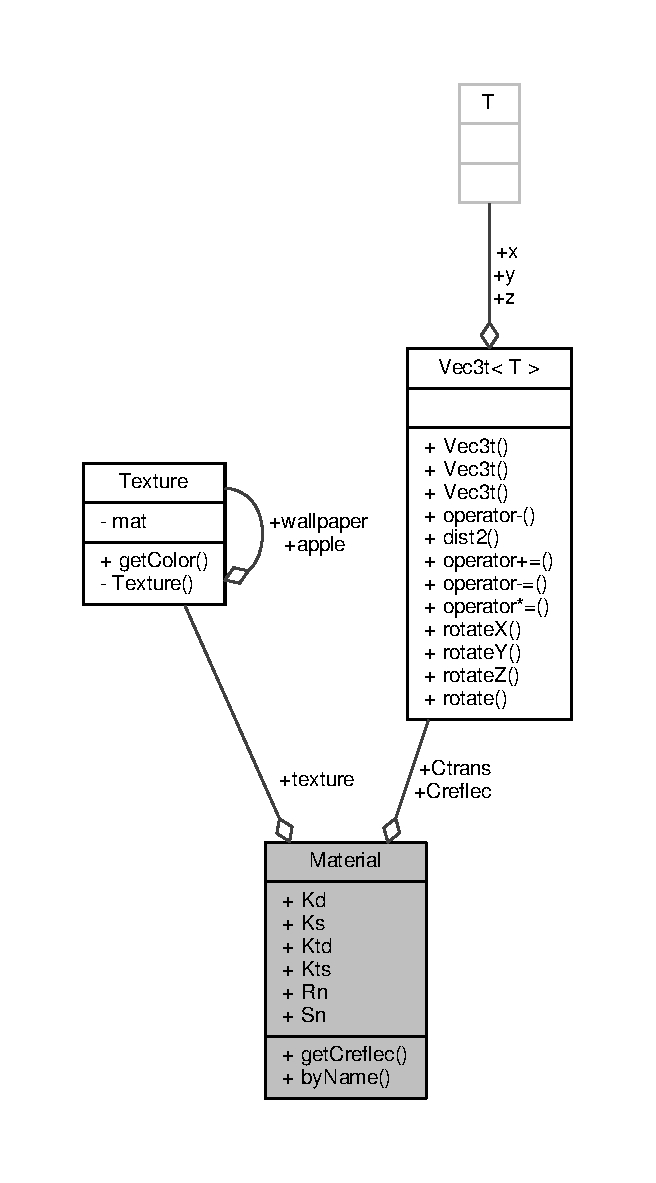
\includegraphics[height=550pt]{structMaterial__coll__graph}
\end{center}
\end{figure}
\subsection*{Public Types}
\begin{DoxyCompactItemize}
\item 
enum \hyperlink{structMaterial_afca902ab9d34ae538cf8eb74afe51911}{Material\+Name} \{ \\*
\hyperlink{structMaterial_afca902ab9d34ae538cf8eb74afe51911aafad09ef73f6aaa26e1dc8bee89871f4}{G\+L\+A\+SS} = 0, 
\hyperlink{structMaterial_afca902ab9d34ae538cf8eb74afe51911aa2ff05704fdd8947102f11cc6b900524}{P\+A\+P\+ER} = 1, 
\hyperlink{structMaterial_afca902ab9d34ae538cf8eb74afe51911adf626c4a22b6e4ebaf71c865f3745511}{W\+A\+L\+L\+P\+A\+P\+ER} = 2, 
\hyperlink{structMaterial_afca902ab9d34ae538cf8eb74afe51911a2589b47b8d5b8e31f37f5cfa05eba139}{F\+R\+O\+S\+T\+E\+D\+\_\+\+G\+L\+A\+SS} = 3, 
\\*
\hyperlink{structMaterial_afca902ab9d34ae538cf8eb74afe51911aa6a166ca282ccb460f6d6f15ba84330c}{M\+A\+T\+EL} = 4, 
\hyperlink{structMaterial_afca902ab9d34ae538cf8eb74afe51911ab6c2ef78c1a421123d7e28eedc85537e}{A\+P\+P\+L\+E1} = 5, 
\hyperlink{structMaterial_afca902ab9d34ae538cf8eb74afe51911a776beb5fcd46544f77f4295e757a66e5}{A\+P\+P\+L\+E2} = 6, 
\hyperlink{structMaterial_afca902ab9d34ae538cf8eb74afe51911a0af45e90f770ebcd117f33e9a902ea21}{C\+A\+R\+P\+ET} = 7, 
\\*
\hyperlink{structMaterial_afca902ab9d34ae538cf8eb74afe51911ac7607d77ae775a5b04874bda2cb82a2e}{I\+N\+V\+A\+L\+ID} = -\/1
 \}
\end{DoxyCompactItemize}
\subsection*{Public Member Functions}
\begin{DoxyCompactItemize}
\item 
\hyperlink{ray_8h_a8a2580fb65f7d3d4e24bdd412b9bd92d}{color\+\_\+t} \hyperlink{structMaterial_a4ab05a2f4f22025aee4c5087a3517d48}{get\+Creflec} (float u, float v) const 
\end{DoxyCompactItemize}
\subsection*{Static Public Member Functions}
\begin{DoxyCompactItemize}
\item 
static \hyperlink{structMaterial}{Material} \hyperlink{structMaterial_ad488bda0cf014154f97bce06b1c3be29}{by\+Name} (\hyperlink{structMaterial_afca902ab9d34ae538cf8eb74afe51911}{Material\+Name} name)
\end{DoxyCompactItemize}
\subsection*{Public Attributes}
\begin{DoxyCompactItemize}
\item 
float \hyperlink{structMaterial_a2db17351a8e462cc446520ae49e64350}{Kd}
\item 
float \hyperlink{structMaterial_acb75581ad97c1df67172d7d7ec59903d}{Ks}
\begin{DoxyCompactList}\small\item\em Diffuse reflection rate. \end{DoxyCompactList}\item 
float \hyperlink{structMaterial_adea51e78c45979bbbb46f04112ea133c}{Ktd}
\begin{DoxyCompactList}\small\item\em Specular relection rate. \end{DoxyCompactList}\item 
float \hyperlink{structMaterial_a75cacce03b4ccb56d436cc188f75ec0f}{Kts}
\begin{DoxyCompactList}\small\item\em Diffuse transition rate. \end{DoxyCompactList}\item 
float \hyperlink{structMaterial_a36c703d1fd25f5c21d9c30e8b403d849}{Rn}
\begin{DoxyCompactList}\small\item\em Specular transition rate. \end{DoxyCompactList}\item 
int \hyperlink{structMaterial_aa45a0497e5baffcebbbe13d5b737f353}{Sn}
\begin{DoxyCompactList}\small\item\em Refrection rate. \end{DoxyCompactList}\item 
\hyperlink{ray_8h_a8a2580fb65f7d3d4e24bdd412b9bd92d}{color\+\_\+t} \hyperlink{structMaterial_a9bc38e4305511b6b74a0df019317be0a}{Creflec}
\begin{DoxyCompactList}\small\item\em Smoothness index (exponent) \end{DoxyCompactList}\item 
\hyperlink{ray_8h_a8a2580fb65f7d3d4e24bdd412b9bd92d}{color\+\_\+t} \hyperlink{structMaterial_aca86e404d70ef98b5c1e466c9c20cee3}{Ctrans}
\begin{DoxyCompactList}\small\item\em Reflection color factor. Actual color = Creflec $\ast$ (Kd or Ks) \end{DoxyCompactList}\item 
\hyperlink{classTexture}{Texture} $\ast$ \hyperlink{structMaterial_ad151148dc3460f25435e951786171350}{texture}
\begin{DoxyCompactList}\small\item\em Transition color factor. Actual color = Ctrans $\ast$ (Ktd or Kts) \end{DoxyCompactList}\end{DoxyCompactItemize}


\subsection{Member Enumeration Documentation}
\index{Material@{Material}!Material\+Name@{Material\+Name}}
\index{Material\+Name@{Material\+Name}!Material@{Material}}
\subsubsection[{\texorpdfstring{Material\+Name}{MaterialName}}]{\setlength{\rightskip}{0pt plus 5cm}enum {\bf Material\+::\+Material\+Name}}\hypertarget{structMaterial_afca902ab9d34ae538cf8eb74afe51911}{}\label{structMaterial_afca902ab9d34ae538cf8eb74afe51911}
\begin{Desc}
\item[Enumerator]\par
\begin{description}
\index{G\+L\+A\+SS@{G\+L\+A\+SS}!Material@{Material}}\index{Material@{Material}!G\+L\+A\+SS@{G\+L\+A\+SS}}\item[{\em 
G\+L\+A\+SS\hypertarget{structMaterial_afca902ab9d34ae538cf8eb74afe51911aafad09ef73f6aaa26e1dc8bee89871f4}{}\label{structMaterial_afca902ab9d34ae538cf8eb74afe51911aafad09ef73f6aaa26e1dc8bee89871f4}
}]\index{P\+A\+P\+ER@{P\+A\+P\+ER}!Material@{Material}}\index{Material@{Material}!P\+A\+P\+ER@{P\+A\+P\+ER}}\item[{\em 
P\+A\+P\+ER\hypertarget{structMaterial_afca902ab9d34ae538cf8eb74afe51911aa2ff05704fdd8947102f11cc6b900524}{}\label{structMaterial_afca902ab9d34ae538cf8eb74afe51911aa2ff05704fdd8947102f11cc6b900524}
}]\index{W\+A\+L\+L\+P\+A\+P\+ER@{W\+A\+L\+L\+P\+A\+P\+ER}!Material@{Material}}\index{Material@{Material}!W\+A\+L\+L\+P\+A\+P\+ER@{W\+A\+L\+L\+P\+A\+P\+ER}}\item[{\em 
W\+A\+L\+L\+P\+A\+P\+ER\hypertarget{structMaterial_afca902ab9d34ae538cf8eb74afe51911adf626c4a22b6e4ebaf71c865f3745511}{}\label{structMaterial_afca902ab9d34ae538cf8eb74afe51911adf626c4a22b6e4ebaf71c865f3745511}
}]\index{F\+R\+O\+S\+T\+E\+D\+\_\+\+G\+L\+A\+SS@{F\+R\+O\+S\+T\+E\+D\+\_\+\+G\+L\+A\+SS}!Material@{Material}}\index{Material@{Material}!F\+R\+O\+S\+T\+E\+D\+\_\+\+G\+L\+A\+SS@{F\+R\+O\+S\+T\+E\+D\+\_\+\+G\+L\+A\+SS}}\item[{\em 
F\+R\+O\+S\+T\+E\+D\+\_\+\+G\+L\+A\+SS\hypertarget{structMaterial_afca902ab9d34ae538cf8eb74afe51911a2589b47b8d5b8e31f37f5cfa05eba139}{}\label{structMaterial_afca902ab9d34ae538cf8eb74afe51911a2589b47b8d5b8e31f37f5cfa05eba139}
}]\index{M\+A\+T\+EL@{M\+A\+T\+EL}!Material@{Material}}\index{Material@{Material}!M\+A\+T\+EL@{M\+A\+T\+EL}}\item[{\em 
M\+A\+T\+EL\hypertarget{structMaterial_afca902ab9d34ae538cf8eb74afe51911aa6a166ca282ccb460f6d6f15ba84330c}{}\label{structMaterial_afca902ab9d34ae538cf8eb74afe51911aa6a166ca282ccb460f6d6f15ba84330c}
}]\index{A\+P\+P\+L\+E1@{A\+P\+P\+L\+E1}!Material@{Material}}\index{Material@{Material}!A\+P\+P\+L\+E1@{A\+P\+P\+L\+E1}}\item[{\em 
A\+P\+P\+L\+E1\hypertarget{structMaterial_afca902ab9d34ae538cf8eb74afe51911ab6c2ef78c1a421123d7e28eedc85537e}{}\label{structMaterial_afca902ab9d34ae538cf8eb74afe51911ab6c2ef78c1a421123d7e28eedc85537e}
}]\index{A\+P\+P\+L\+E2@{A\+P\+P\+L\+E2}!Material@{Material}}\index{Material@{Material}!A\+P\+P\+L\+E2@{A\+P\+P\+L\+E2}}\item[{\em 
A\+P\+P\+L\+E2\hypertarget{structMaterial_afca902ab9d34ae538cf8eb74afe51911a776beb5fcd46544f77f4295e757a66e5}{}\label{structMaterial_afca902ab9d34ae538cf8eb74afe51911a776beb5fcd46544f77f4295e757a66e5}
}]\index{C\+A\+R\+P\+ET@{C\+A\+R\+P\+ET}!Material@{Material}}\index{Material@{Material}!C\+A\+R\+P\+ET@{C\+A\+R\+P\+ET}}\item[{\em 
C\+A\+R\+P\+ET\hypertarget{structMaterial_afca902ab9d34ae538cf8eb74afe51911a0af45e90f770ebcd117f33e9a902ea21}{}\label{structMaterial_afca902ab9d34ae538cf8eb74afe51911a0af45e90f770ebcd117f33e9a902ea21}
}]\index{I\+N\+V\+A\+L\+ID@{I\+N\+V\+A\+L\+ID}!Material@{Material}}\index{Material@{Material}!I\+N\+V\+A\+L\+ID@{I\+N\+V\+A\+L\+ID}}\item[{\em 
I\+N\+V\+A\+L\+ID\hypertarget{structMaterial_afca902ab9d34ae538cf8eb74afe51911ac7607d77ae775a5b04874bda2cb82a2e}{}\label{structMaterial_afca902ab9d34ae538cf8eb74afe51911ac7607d77ae775a5b04874bda2cb82a2e}
}]\end{description}
\end{Desc}


\subsection{Member Function Documentation}
\index{Material@{Material}!by\+Name@{by\+Name}}
\index{by\+Name@{by\+Name}!Material@{Material}}
\subsubsection[{\texorpdfstring{by\+Name(\+Material\+Name name)}{byName(MaterialName name)}}]{\setlength{\rightskip}{0pt plus 5cm}static {\bf Material} Material\+::by\+Name (
\begin{DoxyParamCaption}
\item[{{\bf Material\+Name}}]{name}
\end{DoxyParamCaption}
)\hspace{0.3cm}{\ttfamily [inline]}, {\ttfamily [static]}}\hypertarget{structMaterial_ad488bda0cf014154f97bce06b1c3be29}{}\label{structMaterial_ad488bda0cf014154f97bce06b1c3be29}
\index{Material@{Material}!get\+Creflec@{get\+Creflec}}
\index{get\+Creflec@{get\+Creflec}!Material@{Material}}
\subsubsection[{\texorpdfstring{get\+Creflec(float u, float v) const }{getCreflec(float u, float v) const }}]{\setlength{\rightskip}{0pt plus 5cm}{\bf color\+\_\+t} Material\+::get\+Creflec (
\begin{DoxyParamCaption}
\item[{float}]{u, }
\item[{float}]{v}
\end{DoxyParamCaption}
) const\hspace{0.3cm}{\ttfamily [inline]}}\hypertarget{structMaterial_a4ab05a2f4f22025aee4c5087a3517d48}{}\label{structMaterial_a4ab05a2f4f22025aee4c5087a3517d48}


\subsection{Member Data Documentation}
\index{Material@{Material}!Creflec@{Creflec}}
\index{Creflec@{Creflec}!Material@{Material}}
\subsubsection[{\texorpdfstring{Creflec}{Creflec}}]{\setlength{\rightskip}{0pt plus 5cm}{\bf color\+\_\+t} Material\+::\+Creflec}\hypertarget{structMaterial_a9bc38e4305511b6b74a0df019317be0a}{}\label{structMaterial_a9bc38e4305511b6b74a0df019317be0a}


Smoothness index (exponent) 

\index{Material@{Material}!Ctrans@{Ctrans}}
\index{Ctrans@{Ctrans}!Material@{Material}}
\subsubsection[{\texorpdfstring{Ctrans}{Ctrans}}]{\setlength{\rightskip}{0pt plus 5cm}{\bf color\+\_\+t} Material\+::\+Ctrans}\hypertarget{structMaterial_aca86e404d70ef98b5c1e466c9c20cee3}{}\label{structMaterial_aca86e404d70ef98b5c1e466c9c20cee3}


Reflection color factor. Actual color = Creflec $\ast$ (Kd or Ks) 

\index{Material@{Material}!Kd@{Kd}}
\index{Kd@{Kd}!Material@{Material}}
\subsubsection[{\texorpdfstring{Kd}{Kd}}]{\setlength{\rightskip}{0pt plus 5cm}float Material\+::\+Kd}\hypertarget{structMaterial_a2db17351a8e462cc446520ae49e64350}{}\label{structMaterial_a2db17351a8e462cc446520ae49e64350}
\index{Material@{Material}!Ks@{Ks}}
\index{Ks@{Ks}!Material@{Material}}
\subsubsection[{\texorpdfstring{Ks}{Ks}}]{\setlength{\rightskip}{0pt plus 5cm}float Material\+::\+Ks}\hypertarget{structMaterial_acb75581ad97c1df67172d7d7ec59903d}{}\label{structMaterial_acb75581ad97c1df67172d7d7ec59903d}


Diffuse reflection rate. 

\index{Material@{Material}!Ktd@{Ktd}}
\index{Ktd@{Ktd}!Material@{Material}}
\subsubsection[{\texorpdfstring{Ktd}{Ktd}}]{\setlength{\rightskip}{0pt plus 5cm}float Material\+::\+Ktd}\hypertarget{structMaterial_adea51e78c45979bbbb46f04112ea133c}{}\label{structMaterial_adea51e78c45979bbbb46f04112ea133c}


Specular relection rate. 

\index{Material@{Material}!Kts@{Kts}}
\index{Kts@{Kts}!Material@{Material}}
\subsubsection[{\texorpdfstring{Kts}{Kts}}]{\setlength{\rightskip}{0pt plus 5cm}float Material\+::\+Kts}\hypertarget{structMaterial_a75cacce03b4ccb56d436cc188f75ec0f}{}\label{structMaterial_a75cacce03b4ccb56d436cc188f75ec0f}


Diffuse transition rate. 

\index{Material@{Material}!Rn@{Rn}}
\index{Rn@{Rn}!Material@{Material}}
\subsubsection[{\texorpdfstring{Rn}{Rn}}]{\setlength{\rightskip}{0pt plus 5cm}float Material\+::\+Rn}\hypertarget{structMaterial_a36c703d1fd25f5c21d9c30e8b403d849}{}\label{structMaterial_a36c703d1fd25f5c21d9c30e8b403d849}


Specular transition rate. 

\index{Material@{Material}!Sn@{Sn}}
\index{Sn@{Sn}!Material@{Material}}
\subsubsection[{\texorpdfstring{Sn}{Sn}}]{\setlength{\rightskip}{0pt plus 5cm}int Material\+::\+Sn}\hypertarget{structMaterial_aa45a0497e5baffcebbbe13d5b737f353}{}\label{structMaterial_aa45a0497e5baffcebbbe13d5b737f353}


Refrection rate. 

\index{Material@{Material}!texture@{texture}}
\index{texture@{texture}!Material@{Material}}
\subsubsection[{\texorpdfstring{texture}{texture}}]{\setlength{\rightskip}{0pt plus 5cm}{\bf Texture}$\ast$ Material\+::texture}\hypertarget{structMaterial_ad151148dc3460f25435e951786171350}{}\label{structMaterial_ad151148dc3460f25435e951786171350}


Transition color factor. Actual color = Ctrans $\ast$ (Ktd or Kts) 



The documentation for this struct was generated from the following file\+:\begin{DoxyCompactItemize}
\item 
\hyperlink{material_8h}{material.\+h}\end{DoxyCompactItemize}

\hypertarget{classMesh}{}\section{Mesh Class Reference}
\label{classMesh}\index{Mesh@{Mesh}}


Class used to manage outputing to obj file This is a static class.  




{\ttfamily \#include $<$mesh.\+h$>$}



Collaboration diagram for Mesh\+:\nopagebreak
\begin{figure}[H]
\begin{center}
\leavevmode
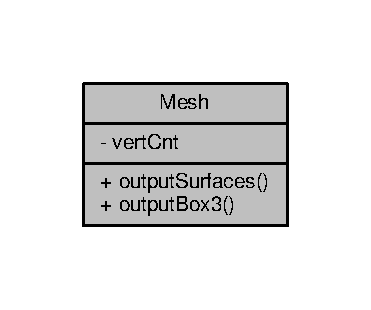
\includegraphics[width=178pt]{classMesh__coll__graph}
\end{center}
\end{figure}
\subsection*{Static Public Member Functions}
\begin{DoxyCompactItemize}
\item 
static void \hyperlink{classMesh_a054505fe7c3b40ff3d822ecf8b43a156}{output\+Surfaces} (std\+::ostream \&os)
\begin{DoxyCompactList}\small\item\em Output all surfaces as meshes. \end{DoxyCompactList}\item 
static void \hyperlink{classMesh_aae0fa0f7959e6dc362025e3d0ade76b7}{output\+Box3} (std\+::ostream \&os, const \hyperlink{structBox3}{Box3} \&box)
\begin{DoxyCompactList}\small\item\em Output a 3D Box. For debugging. \end{DoxyCompactList}\end{DoxyCompactItemize}
\subsection*{Static Private Attributes}
\begin{DoxyCompactItemize}
\item 
static int \hyperlink{classMesh_a4d39ee3e6f94b387fa5b611e4acdf492}{vert\+Cnt} = 0
\end{DoxyCompactItemize}


\subsection{Detailed Description}
Class used to manage outputing to obj file This is a static class. 

\subsection{Member Function Documentation}
\index{Mesh@{Mesh}!output\+Box3@{output\+Box3}}
\index{output\+Box3@{output\+Box3}!Mesh@{Mesh}}
\subsubsection[{\texorpdfstring{output\+Box3(std\+::ostream \&os, const Box3 \&box)}{outputBox3(std::ostream &os, const Box3 &box)}}]{\setlength{\rightskip}{0pt plus 5cm}static void Mesh\+::output\+Box3 (
\begin{DoxyParamCaption}
\item[{std\+::ostream \&}]{os, }
\item[{const {\bf Box3} \&}]{box}
\end{DoxyParamCaption}
)\hspace{0.3cm}{\ttfamily [static]}}\hypertarget{classMesh_aae0fa0f7959e6dc362025e3d0ade76b7}{}\label{classMesh_aae0fa0f7959e6dc362025e3d0ade76b7}


Output a 3D Box. For debugging. 

\index{Mesh@{Mesh}!output\+Surfaces@{output\+Surfaces}}
\index{output\+Surfaces@{output\+Surfaces}!Mesh@{Mesh}}
\subsubsection[{\texorpdfstring{output\+Surfaces(std\+::ostream \&os)}{outputSurfaces(std::ostream &os)}}]{\setlength{\rightskip}{0pt plus 5cm}void Mesh\+::output\+Surfaces (
\begin{DoxyParamCaption}
\item[{std\+::ostream \&}]{os}
\end{DoxyParamCaption}
)\hspace{0.3cm}{\ttfamily [static]}}\hypertarget{classMesh_a054505fe7c3b40ff3d822ecf8b43a156}{}\label{classMesh_a054505fe7c3b40ff3d822ecf8b43a156}


Output all surfaces as meshes. 



\subsection{Member Data Documentation}
\index{Mesh@{Mesh}!vert\+Cnt@{vert\+Cnt}}
\index{vert\+Cnt@{vert\+Cnt}!Mesh@{Mesh}}
\subsubsection[{\texorpdfstring{vert\+Cnt}{vertCnt}}]{\setlength{\rightskip}{0pt plus 5cm}int Mesh\+::vert\+Cnt = 0\hspace{0.3cm}{\ttfamily [static]}, {\ttfamily [private]}}\hypertarget{classMesh_a4d39ee3e6f94b387fa5b611e4acdf492}{}\label{classMesh_a4d39ee3e6f94b387fa5b611e4acdf492}


The documentation for this class was generated from the following files\+:\begin{DoxyCompactItemize}
\item 
\hyperlink{mesh_8h}{mesh.\+h}\item 
\hyperlink{mesh_8cpp}{mesh.\+cpp}\end{DoxyCompactItemize}

\hypertarget{structBoxTree_1_1Node}{}\section{Box\+Tree\+:\+:Node Struct Reference}
\label{structBoxTree_1_1Node}\index{Box\+Tree\+::\+Node@{Box\+Tree\+::\+Node}}


{\ttfamily \#include $<$boxtree.\+h$>$}



Collaboration diagram for Box\+Tree\+:\+:Node\+:
\nopagebreak
\begin{figure}[H]
\begin{center}
\leavevmode
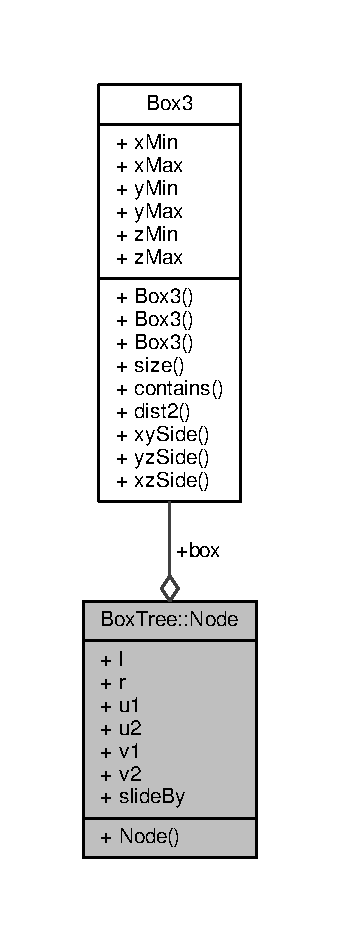
\includegraphics[width=163pt]{structBoxTree_1_1Node__coll__graph}
\end{center}
\end{figure}
\subsection*{Public Types}
\begin{DoxyCompactItemize}
\item 
enum \hyperlink{structBoxTree_1_1Node_af862522c79bbea75bbbfa47614842295}{Slide\+Dir} \{ \hyperlink{structBoxTree_1_1Node_af862522c79bbea75bbbfa47614842295a8de683397fda85467d10531bdaf67577}{B\+Y\+\_\+U} = 0, 
\hyperlink{structBoxTree_1_1Node_af862522c79bbea75bbbfa47614842295acd6e4816ec952840b6cd2dc8261a3963}{B\+Y\+\_\+V} = 1, 
\hyperlink{structBoxTree_1_1Node_af862522c79bbea75bbbfa47614842295a06e0ae6f4066175d8a5739b775f52c83}{L\+E\+AF} = -\/1
 \}
\end{DoxyCompactItemize}
\subsection*{Public Member Functions}
\begin{DoxyCompactItemize}
\item 
\hyperlink{structBoxTree_1_1Node_a9b631d5d7dd608857dbf6b16407b1e0a}{Node} (float \+\_\+u1, float \+\_\+u2, float \+\_\+v1, float \+\_\+v2, const \hyperlink{structBox3}{Box3} \&\+\_\+box)
\end{DoxyCompactItemize}
\subsection*{Public Attributes}
\begin{DoxyCompactItemize}
\item 
std\+::unique\+\_\+ptr$<$ \hyperlink{structBoxTree_1_1Node}{Node} $>$ \hyperlink{structBoxTree_1_1Node_a9d101fa1093b0c23cbff294f65c0a04b}{l}
\item 
std\+::unique\+\_\+ptr$<$ \hyperlink{structBoxTree_1_1Node}{Node} $>$ \hyperlink{structBoxTree_1_1Node_a8e85cff13a1049196ff4457654c9fa33}{r}
\item 
float \hyperlink{structBoxTree_1_1Node_ab92350a00f11c1d1f7c7c076029bfa65}{u1}
\begin{DoxyCompactList}\small\item\em children \end{DoxyCompactList}\item 
float \hyperlink{structBoxTree_1_1Node_a5f00089be77fb8baf47bde296a491a5b}{u2}
\item 
float \hyperlink{structBoxTree_1_1Node_a6776d4995a710d07a91c8ce29d6ca8e8}{v1}
\item 
float \hyperlink{structBoxTree_1_1Node_a00397c546d573ed0018f43b714414303}{v2}
\item 
\hyperlink{structBox3}{Box3} \hyperlink{structBoxTree_1_1Node_a0926dd1c5b248667de3399a08bf6bc6f}{box}
\item 
\hyperlink{structBoxTree_1_1Node_af862522c79bbea75bbbfa47614842295}{Slide\+Dir} \hyperlink{structBoxTree_1_1Node_a23938b7d422df4c0faebd8fe0af43bd3}{slide\+By}
\end{DoxyCompactItemize}


\subsection{Member Enumeration Documentation}
\index{Box\+Tree\+::\+Node@{Box\+Tree\+::\+Node}!Slide\+Dir@{Slide\+Dir}}
\index{Slide\+Dir@{Slide\+Dir}!Box\+Tree\+::\+Node@{Box\+Tree\+::\+Node}}
\subsubsection[{\texorpdfstring{Slide\+Dir}{SlideDir}}]{\setlength{\rightskip}{0pt plus 5cm}enum {\bf Box\+Tree\+::\+Node\+::\+Slide\+Dir}}\hypertarget{structBoxTree_1_1Node_af862522c79bbea75bbbfa47614842295}{}\label{structBoxTree_1_1Node_af862522c79bbea75bbbfa47614842295}
\begin{Desc}
\item[Enumerator]\par
\begin{description}
\index{B\+Y\+\_\+U@{B\+Y\+\_\+U}!Box\+Tree\+::\+Node@{Box\+Tree\+::\+Node}}\index{Box\+Tree\+::\+Node@{Box\+Tree\+::\+Node}!B\+Y\+\_\+U@{B\+Y\+\_\+U}}\item[{\em 
B\+Y\+\_\+U\hypertarget{structBoxTree_1_1Node_af862522c79bbea75bbbfa47614842295a8de683397fda85467d10531bdaf67577}{}\label{structBoxTree_1_1Node_af862522c79bbea75bbbfa47614842295a8de683397fda85467d10531bdaf67577}
}]\index{B\+Y\+\_\+V@{B\+Y\+\_\+V}!Box\+Tree\+::\+Node@{Box\+Tree\+::\+Node}}\index{Box\+Tree\+::\+Node@{Box\+Tree\+::\+Node}!B\+Y\+\_\+V@{B\+Y\+\_\+V}}\item[{\em 
B\+Y\+\_\+V\hypertarget{structBoxTree_1_1Node_af862522c79bbea75bbbfa47614842295acd6e4816ec952840b6cd2dc8261a3963}{}\label{structBoxTree_1_1Node_af862522c79bbea75bbbfa47614842295acd6e4816ec952840b6cd2dc8261a3963}
}]\index{L\+E\+AF@{L\+E\+AF}!Box\+Tree\+::\+Node@{Box\+Tree\+::\+Node}}\index{Box\+Tree\+::\+Node@{Box\+Tree\+::\+Node}!L\+E\+AF@{L\+E\+AF}}\item[{\em 
L\+E\+AF\hypertarget{structBoxTree_1_1Node_af862522c79bbea75bbbfa47614842295a06e0ae6f4066175d8a5739b775f52c83}{}\label{structBoxTree_1_1Node_af862522c79bbea75bbbfa47614842295a06e0ae6f4066175d8a5739b775f52c83}
}]\end{description}
\end{Desc}


\subsection{Constructor \& Destructor Documentation}
\index{Box\+Tree\+::\+Node@{Box\+Tree\+::\+Node}!Node@{Node}}
\index{Node@{Node}!Box\+Tree\+::\+Node@{Box\+Tree\+::\+Node}}
\subsubsection[{\texorpdfstring{Node(float \+\_\+u1, float \+\_\+u2, float \+\_\+v1, float \+\_\+v2, const Box3 \&\+\_\+box)}{Node(float _u1, float _u2, float _v1, float _v2, const Box3 &_box)}}]{\setlength{\rightskip}{0pt plus 5cm}Box\+Tree\+::\+Node\+::\+Node (
\begin{DoxyParamCaption}
\item[{float}]{\+\_\+u1, }
\item[{float}]{\+\_\+u2, }
\item[{float}]{\+\_\+v1, }
\item[{float}]{\+\_\+v2, }
\item[{const {\bf Box3} \&}]{\+\_\+box}
\end{DoxyParamCaption}
)\hspace{0.3cm}{\ttfamily [inline]}}\hypertarget{structBoxTree_1_1Node_a9b631d5d7dd608857dbf6b16407b1e0a}{}\label{structBoxTree_1_1Node_a9b631d5d7dd608857dbf6b16407b1e0a}


\subsection{Member Data Documentation}
\index{Box\+Tree\+::\+Node@{Box\+Tree\+::\+Node}!box@{box}}
\index{box@{box}!Box\+Tree\+::\+Node@{Box\+Tree\+::\+Node}}
\subsubsection[{\texorpdfstring{box}{box}}]{\setlength{\rightskip}{0pt plus 5cm}{\bf Box3} Box\+Tree\+::\+Node\+::box}\hypertarget{structBoxTree_1_1Node_a0926dd1c5b248667de3399a08bf6bc6f}{}\label{structBoxTree_1_1Node_a0926dd1c5b248667de3399a08bf6bc6f}
\index{Box\+Tree\+::\+Node@{Box\+Tree\+::\+Node}!l@{l}}
\index{l@{l}!Box\+Tree\+::\+Node@{Box\+Tree\+::\+Node}}
\subsubsection[{\texorpdfstring{l}{l}}]{\setlength{\rightskip}{0pt plus 5cm}std\+::unique\+\_\+ptr$<${\bf Node}$>$ Box\+Tree\+::\+Node\+::l}\hypertarget{structBoxTree_1_1Node_a9d101fa1093b0c23cbff294f65c0a04b}{}\label{structBoxTree_1_1Node_a9d101fa1093b0c23cbff294f65c0a04b}
\index{Box\+Tree\+::\+Node@{Box\+Tree\+::\+Node}!r@{r}}
\index{r@{r}!Box\+Tree\+::\+Node@{Box\+Tree\+::\+Node}}
\subsubsection[{\texorpdfstring{r}{r}}]{\setlength{\rightskip}{0pt plus 5cm}std\+::unique\+\_\+ptr$<${\bf Node}$>$ Box\+Tree\+::\+Node\+::r}\hypertarget{structBoxTree_1_1Node_a8e85cff13a1049196ff4457654c9fa33}{}\label{structBoxTree_1_1Node_a8e85cff13a1049196ff4457654c9fa33}
\index{Box\+Tree\+::\+Node@{Box\+Tree\+::\+Node}!slide\+By@{slide\+By}}
\index{slide\+By@{slide\+By}!Box\+Tree\+::\+Node@{Box\+Tree\+::\+Node}}
\subsubsection[{\texorpdfstring{slide\+By}{slideBy}}]{\setlength{\rightskip}{0pt plus 5cm}{\bf Slide\+Dir} Box\+Tree\+::\+Node\+::slide\+By}\hypertarget{structBoxTree_1_1Node_a23938b7d422df4c0faebd8fe0af43bd3}{}\label{structBoxTree_1_1Node_a23938b7d422df4c0faebd8fe0af43bd3}
\index{Box\+Tree\+::\+Node@{Box\+Tree\+::\+Node}!u1@{u1}}
\index{u1@{u1}!Box\+Tree\+::\+Node@{Box\+Tree\+::\+Node}}
\subsubsection[{\texorpdfstring{u1}{u1}}]{\setlength{\rightskip}{0pt plus 5cm}float Box\+Tree\+::\+Node\+::u1}\hypertarget{structBoxTree_1_1Node_ab92350a00f11c1d1f7c7c076029bfa65}{}\label{structBoxTree_1_1Node_ab92350a00f11c1d1f7c7c076029bfa65}


children 

\index{Box\+Tree\+::\+Node@{Box\+Tree\+::\+Node}!u2@{u2}}
\index{u2@{u2}!Box\+Tree\+::\+Node@{Box\+Tree\+::\+Node}}
\subsubsection[{\texorpdfstring{u2}{u2}}]{\setlength{\rightskip}{0pt plus 5cm}float Box\+Tree\+::\+Node\+::u2}\hypertarget{structBoxTree_1_1Node_a5f00089be77fb8baf47bde296a491a5b}{}\label{structBoxTree_1_1Node_a5f00089be77fb8baf47bde296a491a5b}
\index{Box\+Tree\+::\+Node@{Box\+Tree\+::\+Node}!v1@{v1}}
\index{v1@{v1}!Box\+Tree\+::\+Node@{Box\+Tree\+::\+Node}}
\subsubsection[{\texorpdfstring{v1}{v1}}]{\setlength{\rightskip}{0pt plus 5cm}float Box\+Tree\+::\+Node\+::v1}\hypertarget{structBoxTree_1_1Node_a6776d4995a710d07a91c8ce29d6ca8e8}{}\label{structBoxTree_1_1Node_a6776d4995a710d07a91c8ce29d6ca8e8}
\index{Box\+Tree\+::\+Node@{Box\+Tree\+::\+Node}!v2@{v2}}
\index{v2@{v2}!Box\+Tree\+::\+Node@{Box\+Tree\+::\+Node}}
\subsubsection[{\texorpdfstring{v2}{v2}}]{\setlength{\rightskip}{0pt plus 5cm}float Box\+Tree\+::\+Node\+::v2}\hypertarget{structBoxTree_1_1Node_a00397c546d573ed0018f43b714414303}{}\label{structBoxTree_1_1Node_a00397c546d573ed0018f43b714414303}


The documentation for this struct was generated from the following file\+:\begin{DoxyCompactItemize}
\item 
\hyperlink{boxtree_8h}{boxtree.\+h}\end{DoxyCompactItemize}

\hypertarget{structKDTree_1_1Node}{}\section{K\+D\+Tree\+:\+:Node Struct Reference}
\label{structKDTree_1_1Node}\index{K\+D\+Tree\+::\+Node@{K\+D\+Tree\+::\+Node}}


Collaboration diagram for K\+D\+Tree\+:\+:Node\+:\nopagebreak
\begin{figure}[H]
\begin{center}
\leavevmode
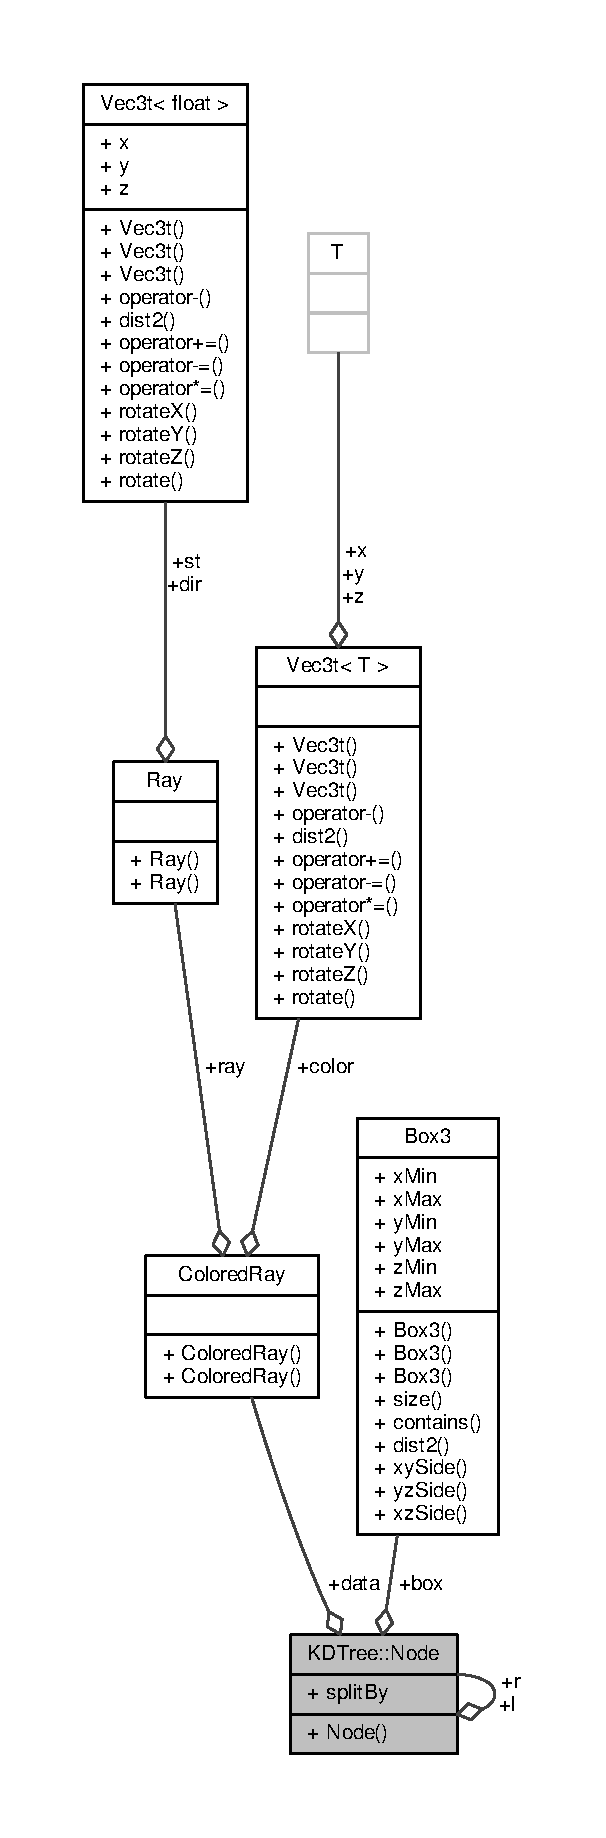
\includegraphics[height=550pt]{structKDTree_1_1Node__coll__graph}
\end{center}
\end{figure}
\subsection*{Public Types}
\begin{DoxyCompactItemize}
\item 
enum \hyperlink{structKDTree_1_1Node_ab21ae38de8fe0e25d29d0ae136a1db34}{split\+\_\+t} \{ \hyperlink{structKDTree_1_1Node_ab21ae38de8fe0e25d29d0ae136a1db34ae9e20517e320a257a7ec3aecb69427ec}{L\+E\+AF} = 0, 
\hyperlink{structKDTree_1_1Node_ab21ae38de8fe0e25d29d0ae136a1db34a36069e5e459835d23e1e4e2412f15f15}{B\+Y\+\_\+X} = 1, 
\hyperlink{structKDTree_1_1Node_ab21ae38de8fe0e25d29d0ae136a1db34a16bcf65fb5fef5f33c18e6de9022fd2d}{B\+Y\+\_\+Y} = 2, 
\hyperlink{structKDTree_1_1Node_ab21ae38de8fe0e25d29d0ae136a1db34a921306d44eb973ea0dffcff75817a095}{B\+Y\+\_\+Z} = 3
 \}
\end{DoxyCompactItemize}
\subsection*{Public Member Functions}
\begin{DoxyCompactItemize}
\item 
\hyperlink{structKDTree_1_1Node_ab83c48d5ca5c7b0aaee2831e8ffcea37}{Node} (const \hyperlink{classKDTree_ab000d86d0fb4aaedcc83b5b7a584c25e}{data\+\_\+t} \&\+\_\+data)
\begin{DoxyCompactList}\small\item\em Children. \end{DoxyCompactList}\end{DoxyCompactItemize}
\subsection*{Public Attributes}
\begin{DoxyCompactItemize}
\item 
enum \hyperlink{structKDTree_1_1Node_ab21ae38de8fe0e25d29d0ae136a1db34}{K\+D\+Tree\+::\+Node\+::split\+\_\+t} \hyperlink{structKDTree_1_1Node_a6ab2edd3f12f7e2f547c55d219252469}{split\+By}
\item 
\hyperlink{classKDTree_ab000d86d0fb4aaedcc83b5b7a584c25e}{data\+\_\+t} \hyperlink{structKDTree_1_1Node_a314e8792d65f995e383f2658f9c9a9d9}{data}
\item 
\hyperlink{structBox3}{Box3} \hyperlink{structKDTree_1_1Node_a71a3c79703c2fac391d11561f05f3bc3}{box}
\begin{DoxyCompactList}\small\item\em Data associated with this node. \end{DoxyCompactList}\item 
\hyperlink{structKDTree_1_1Node}{Node} $\ast$ \hyperlink{structKDTree_1_1Node_a9afeb2a23f401c72e147def1e8f9b133}{l}
\begin{DoxyCompactList}\small\item\em Bounding box of this node. \end{DoxyCompactList}\item 
\hyperlink{structKDTree_1_1Node}{Node} $\ast$ \hyperlink{structKDTree_1_1Node_a1ee516a9562dc5c6f53ad1176c2016a4}{r}
\end{DoxyCompactItemize}


\subsection{Member Enumeration Documentation}
\index{K\+D\+Tree\+::\+Node@{K\+D\+Tree\+::\+Node}!split\+\_\+t@{split\+\_\+t}}
\index{split\+\_\+t@{split\+\_\+t}!K\+D\+Tree\+::\+Node@{K\+D\+Tree\+::\+Node}}
\subsubsection[{\texorpdfstring{split\+\_\+t}{split_t}}]{\setlength{\rightskip}{0pt plus 5cm}enum {\bf K\+D\+Tree\+::\+Node\+::split\+\_\+t}}\hypertarget{structKDTree_1_1Node_ab21ae38de8fe0e25d29d0ae136a1db34}{}\label{structKDTree_1_1Node_ab21ae38de8fe0e25d29d0ae136a1db34}
\begin{Desc}
\item[Enumerator]\par
\begin{description}
\index{L\+E\+AF@{L\+E\+AF}!K\+D\+Tree\+::\+Node@{K\+D\+Tree\+::\+Node}}\index{K\+D\+Tree\+::\+Node@{K\+D\+Tree\+::\+Node}!L\+E\+AF@{L\+E\+AF}}\item[{\em 
L\+E\+AF\hypertarget{structKDTree_1_1Node_ab21ae38de8fe0e25d29d0ae136a1db34ae9e20517e320a257a7ec3aecb69427ec}{}\label{structKDTree_1_1Node_ab21ae38de8fe0e25d29d0ae136a1db34ae9e20517e320a257a7ec3aecb69427ec}
}]\index{B\+Y\+\_\+X@{B\+Y\+\_\+X}!K\+D\+Tree\+::\+Node@{K\+D\+Tree\+::\+Node}}\index{K\+D\+Tree\+::\+Node@{K\+D\+Tree\+::\+Node}!B\+Y\+\_\+X@{B\+Y\+\_\+X}}\item[{\em 
B\+Y\+\_\+X\hypertarget{structKDTree_1_1Node_ab21ae38de8fe0e25d29d0ae136a1db34a36069e5e459835d23e1e4e2412f15f15}{}\label{structKDTree_1_1Node_ab21ae38de8fe0e25d29d0ae136a1db34a36069e5e459835d23e1e4e2412f15f15}
}]\index{B\+Y\+\_\+Y@{B\+Y\+\_\+Y}!K\+D\+Tree\+::\+Node@{K\+D\+Tree\+::\+Node}}\index{K\+D\+Tree\+::\+Node@{K\+D\+Tree\+::\+Node}!B\+Y\+\_\+Y@{B\+Y\+\_\+Y}}\item[{\em 
B\+Y\+\_\+Y\hypertarget{structKDTree_1_1Node_ab21ae38de8fe0e25d29d0ae136a1db34a16bcf65fb5fef5f33c18e6de9022fd2d}{}\label{structKDTree_1_1Node_ab21ae38de8fe0e25d29d0ae136a1db34a16bcf65fb5fef5f33c18e6de9022fd2d}
}]\index{B\+Y\+\_\+Z@{B\+Y\+\_\+Z}!K\+D\+Tree\+::\+Node@{K\+D\+Tree\+::\+Node}}\index{K\+D\+Tree\+::\+Node@{K\+D\+Tree\+::\+Node}!B\+Y\+\_\+Z@{B\+Y\+\_\+Z}}\item[{\em 
B\+Y\+\_\+Z\hypertarget{structKDTree_1_1Node_ab21ae38de8fe0e25d29d0ae136a1db34a921306d44eb973ea0dffcff75817a095}{}\label{structKDTree_1_1Node_ab21ae38de8fe0e25d29d0ae136a1db34a921306d44eb973ea0dffcff75817a095}
}]\end{description}
\end{Desc}


\subsection{Constructor \& Destructor Documentation}
\index{K\+D\+Tree\+::\+Node@{K\+D\+Tree\+::\+Node}!Node@{Node}}
\index{Node@{Node}!K\+D\+Tree\+::\+Node@{K\+D\+Tree\+::\+Node}}
\subsubsection[{\texorpdfstring{Node(const data\+\_\+t \&\+\_\+data)}{Node(const data_t &_data)}}]{\setlength{\rightskip}{0pt plus 5cm}K\+D\+Tree\+::\+Node\+::\+Node (
\begin{DoxyParamCaption}
\item[{const {\bf data\+\_\+t} \&}]{\+\_\+data}
\end{DoxyParamCaption}
)\hspace{0.3cm}{\ttfamily [inline]}}\hypertarget{structKDTree_1_1Node_ab83c48d5ca5c7b0aaee2831e8ffcea37}{}\label{structKDTree_1_1Node_ab83c48d5ca5c7b0aaee2831e8ffcea37}


Children. 



\subsection{Member Data Documentation}
\index{K\+D\+Tree\+::\+Node@{K\+D\+Tree\+::\+Node}!box@{box}}
\index{box@{box}!K\+D\+Tree\+::\+Node@{K\+D\+Tree\+::\+Node}}
\subsubsection[{\texorpdfstring{box}{box}}]{\setlength{\rightskip}{0pt plus 5cm}{\bf Box3} K\+D\+Tree\+::\+Node\+::box}\hypertarget{structKDTree_1_1Node_a71a3c79703c2fac391d11561f05f3bc3}{}\label{structKDTree_1_1Node_a71a3c79703c2fac391d11561f05f3bc3}


Data associated with this node. 

\index{K\+D\+Tree\+::\+Node@{K\+D\+Tree\+::\+Node}!data@{data}}
\index{data@{data}!K\+D\+Tree\+::\+Node@{K\+D\+Tree\+::\+Node}}
\subsubsection[{\texorpdfstring{data}{data}}]{\setlength{\rightskip}{0pt plus 5cm}{\bf data\+\_\+t} K\+D\+Tree\+::\+Node\+::data}\hypertarget{structKDTree_1_1Node_a314e8792d65f995e383f2658f9c9a9d9}{}\label{structKDTree_1_1Node_a314e8792d65f995e383f2658f9c9a9d9}
\index{K\+D\+Tree\+::\+Node@{K\+D\+Tree\+::\+Node}!l@{l}}
\index{l@{l}!K\+D\+Tree\+::\+Node@{K\+D\+Tree\+::\+Node}}
\subsubsection[{\texorpdfstring{l}{l}}]{\setlength{\rightskip}{0pt plus 5cm}{\bf Node}$\ast$ K\+D\+Tree\+::\+Node\+::l}\hypertarget{structKDTree_1_1Node_a9afeb2a23f401c72e147def1e8f9b133}{}\label{structKDTree_1_1Node_a9afeb2a23f401c72e147def1e8f9b133}


Bounding box of this node. 

\index{K\+D\+Tree\+::\+Node@{K\+D\+Tree\+::\+Node}!r@{r}}
\index{r@{r}!K\+D\+Tree\+::\+Node@{K\+D\+Tree\+::\+Node}}
\subsubsection[{\texorpdfstring{r}{r}}]{\setlength{\rightskip}{0pt plus 5cm}{\bf Node} $\ast$ K\+D\+Tree\+::\+Node\+::r}\hypertarget{structKDTree_1_1Node_a1ee516a9562dc5c6f53ad1176c2016a4}{}\label{structKDTree_1_1Node_a1ee516a9562dc5c6f53ad1176c2016a4}
\index{K\+D\+Tree\+::\+Node@{K\+D\+Tree\+::\+Node}!split\+By@{split\+By}}
\index{split\+By@{split\+By}!K\+D\+Tree\+::\+Node@{K\+D\+Tree\+::\+Node}}
\subsubsection[{\texorpdfstring{split\+By}{splitBy}}]{\setlength{\rightskip}{0pt plus 5cm}enum {\bf K\+D\+Tree\+::\+Node\+::split\+\_\+t}  K\+D\+Tree\+::\+Node\+::split\+By}\hypertarget{structKDTree_1_1Node_a6ab2edd3f12f7e2f547c55d219252469}{}\label{structKDTree_1_1Node_a6ab2edd3f12f7e2f547c55d219252469}


The documentation for this struct was generated from the following file\+:\begin{DoxyCompactItemize}
\item 
\hyperlink{kdtree_8h}{kdtree.\+h}\end{DoxyCompactItemize}

\hypertarget{classNone}{}\section{None Class Reference}
\label{classNone}\index{None@{None}}


{\ttfamily \#include $<$optional.\+h$>$}



Collaboration diagram for None\+:
\nopagebreak
\begin{figure}[H]
\begin{center}
\leavevmode
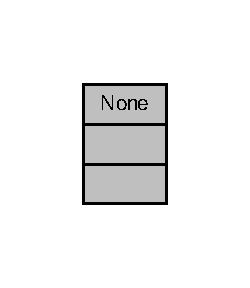
\includegraphics[width=120pt]{classNone__coll__graph}
\end{center}
\end{figure}


The documentation for this class was generated from the following file\+:\begin{DoxyCompactItemize}
\item 
\hyperlink{optional_8h}{optional.\+h}\end{DoxyCompactItemize}

\hypertarget{classOptional}{}\section{Optional$<$ T $>$ Class Template Reference}
\label{classOptional}\index{Optional$<$ T $>$@{Optional$<$ T $>$}}


{\ttfamily \#include $<$optional.\+h$>$}



Collaboration diagram for Optional$<$ T $>$\+:
\nopagebreak
\begin{figure}[H]
\begin{center}
\leavevmode
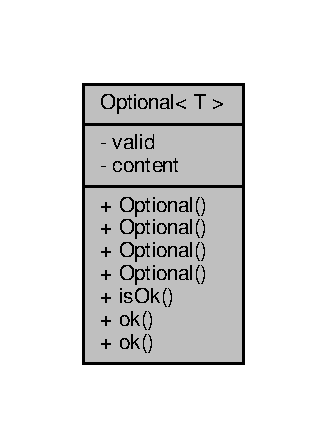
\includegraphics[width=157pt]{classOptional__coll__graph}
\end{center}
\end{figure}
\subsection*{Public Member Functions}
\begin{DoxyCompactItemize}
\item 
\hyperlink{classOptional_a7e936c9ca1669872d5e69ee5b2638088}{Optional} ()
\item 
\hyperlink{classOptional_a3b83f585aaa6a83591a3e32fe70c1087}{Optional} (\hyperlink{classNone}{None})
\item 
\hyperlink{classOptional_a78c5b279afd6400594f25961b927b2db}{Optional} (const T \&\+\_\+content)
\item 
\hyperlink{classOptional_a167b270716a2fed9d345625df0784700}{Optional} (T \&\&\+\_\+content)
\item 
bool \hyperlink{classOptional_a57a690d23369434ecc65d64e8a710b92}{is\+Ok} () const 
\item 
T \& \hyperlink{classOptional_a6527daf92b89333557d6b37938a965f2}{ok} ()
\item 
const T \& \hyperlink{classOptional_a1d5c2fc9361cd4944f8efda048003190}{ok} () const 
\end{DoxyCompactItemize}
\subsection*{Private Attributes}
\begin{DoxyCompactItemize}
\item 
bool \hyperlink{classOptional_a1c0ea9e0a240481b254de9f6cb401882}{valid}
\item 
T \hyperlink{classOptional_a1c694f39ac1ed0deab4ab888b0529746}{content}
\end{DoxyCompactItemize}


\subsection{Constructor \& Destructor Documentation}
\index{Optional@{Optional}!Optional@{Optional}}
\index{Optional@{Optional}!Optional@{Optional}}
\subsubsection[{\texorpdfstring{Optional()}{Optional()}}]{\setlength{\rightskip}{0pt plus 5cm}template$<$class T$>$ {\bf Optional}$<$ T $>$\+::{\bf Optional} (
\begin{DoxyParamCaption}
{}
\end{DoxyParamCaption}
)\hspace{0.3cm}{\ttfamily [inline]}}\hypertarget{classOptional_a7e936c9ca1669872d5e69ee5b2638088}{}\label{classOptional_a7e936c9ca1669872d5e69ee5b2638088}
\index{Optional@{Optional}!Optional@{Optional}}
\index{Optional@{Optional}!Optional@{Optional}}
\subsubsection[{\texorpdfstring{Optional(\+None)}{Optional(None)}}]{\setlength{\rightskip}{0pt plus 5cm}template$<$class T$>$ {\bf Optional}$<$ T $>$\+::{\bf Optional} (
\begin{DoxyParamCaption}
\item[{{\bf None}}]{}
\end{DoxyParamCaption}
)\hspace{0.3cm}{\ttfamily [inline]}}\hypertarget{classOptional_a3b83f585aaa6a83591a3e32fe70c1087}{}\label{classOptional_a3b83f585aaa6a83591a3e32fe70c1087}
\index{Optional@{Optional}!Optional@{Optional}}
\index{Optional@{Optional}!Optional@{Optional}}
\subsubsection[{\texorpdfstring{Optional(const T \&\+\_\+content)}{Optional(const T &_content)}}]{\setlength{\rightskip}{0pt plus 5cm}template$<$class T$>$ {\bf Optional}$<$ T $>$\+::{\bf Optional} (
\begin{DoxyParamCaption}
\item[{const T \&}]{\+\_\+content}
\end{DoxyParamCaption}
)\hspace{0.3cm}{\ttfamily [inline]}}\hypertarget{classOptional_a78c5b279afd6400594f25961b927b2db}{}\label{classOptional_a78c5b279afd6400594f25961b927b2db}
\index{Optional@{Optional}!Optional@{Optional}}
\index{Optional@{Optional}!Optional@{Optional}}
\subsubsection[{\texorpdfstring{Optional(\+T \&\&\+\_\+content)}{Optional(T &&_content)}}]{\setlength{\rightskip}{0pt plus 5cm}template$<$class T$>$ {\bf Optional}$<$ T $>$\+::{\bf Optional} (
\begin{DoxyParamCaption}
\item[{T \&\&}]{\+\_\+content}
\end{DoxyParamCaption}
)\hspace{0.3cm}{\ttfamily [inline]}}\hypertarget{classOptional_a167b270716a2fed9d345625df0784700}{}\label{classOptional_a167b270716a2fed9d345625df0784700}


\subsection{Member Function Documentation}
\index{Optional@{Optional}!is\+Ok@{is\+Ok}}
\index{is\+Ok@{is\+Ok}!Optional@{Optional}}
\subsubsection[{\texorpdfstring{is\+Ok() const }{isOk() const }}]{\setlength{\rightskip}{0pt plus 5cm}template$<$class T$>$ bool {\bf Optional}$<$ T $>$\+::is\+Ok (
\begin{DoxyParamCaption}
{}
\end{DoxyParamCaption}
) const\hspace{0.3cm}{\ttfamily [inline]}}\hypertarget{classOptional_a57a690d23369434ecc65d64e8a710b92}{}\label{classOptional_a57a690d23369434ecc65d64e8a710b92}
\index{Optional@{Optional}!ok@{ok}}
\index{ok@{ok}!Optional@{Optional}}
\subsubsection[{\texorpdfstring{ok()}{ok()}}]{\setlength{\rightskip}{0pt plus 5cm}template$<$class T$>$ T\& {\bf Optional}$<$ T $>$\+::ok (
\begin{DoxyParamCaption}
{}
\end{DoxyParamCaption}
)\hspace{0.3cm}{\ttfamily [inline]}}\hypertarget{classOptional_a6527daf92b89333557d6b37938a965f2}{}\label{classOptional_a6527daf92b89333557d6b37938a965f2}
\index{Optional@{Optional}!ok@{ok}}
\index{ok@{ok}!Optional@{Optional}}
\subsubsection[{\texorpdfstring{ok() const }{ok() const }}]{\setlength{\rightskip}{0pt plus 5cm}template$<$class T$>$ const T\& {\bf Optional}$<$ T $>$\+::ok (
\begin{DoxyParamCaption}
{}
\end{DoxyParamCaption}
) const\hspace{0.3cm}{\ttfamily [inline]}}\hypertarget{classOptional_a1d5c2fc9361cd4944f8efda048003190}{}\label{classOptional_a1d5c2fc9361cd4944f8efda048003190}


\subsection{Member Data Documentation}
\index{Optional@{Optional}!content@{content}}
\index{content@{content}!Optional@{Optional}}
\subsubsection[{\texorpdfstring{content}{content}}]{\setlength{\rightskip}{0pt plus 5cm}template$<$class T$>$ T {\bf Optional}$<$ T $>$\+::content\hspace{0.3cm}{\ttfamily [private]}}\hypertarget{classOptional_a1c694f39ac1ed0deab4ab888b0529746}{}\label{classOptional_a1c694f39ac1ed0deab4ab888b0529746}
\index{Optional@{Optional}!valid@{valid}}
\index{valid@{valid}!Optional@{Optional}}
\subsubsection[{\texorpdfstring{valid}{valid}}]{\setlength{\rightskip}{0pt plus 5cm}template$<$class T$>$ bool {\bf Optional}$<$ T $>$\+::valid\hspace{0.3cm}{\ttfamily [private]}}\hypertarget{classOptional_a1c0ea9e0a240481b254de9f6cb401882}{}\label{classOptional_a1c0ea9e0a240481b254de9f6cb401882}


The documentation for this class was generated from the following file\+:\begin{DoxyCompactItemize}
\item 
\hyperlink{optional_8h}{optional.\+h}\end{DoxyCompactItemize}

\hypertarget{classPhotonMap}{}\section{Photon\+Map Class Reference}
\label{classPhotonMap}\index{Photon\+Map@{Photon\+Map}}


Photon Map Use in order\+: 1.  




{\ttfamily \#include $<$photonmap.\+h$>$}



Collaboration diagram for Photon\+Map\+:
\nopagebreak
\begin{figure}[H]
\begin{center}
\leavevmode
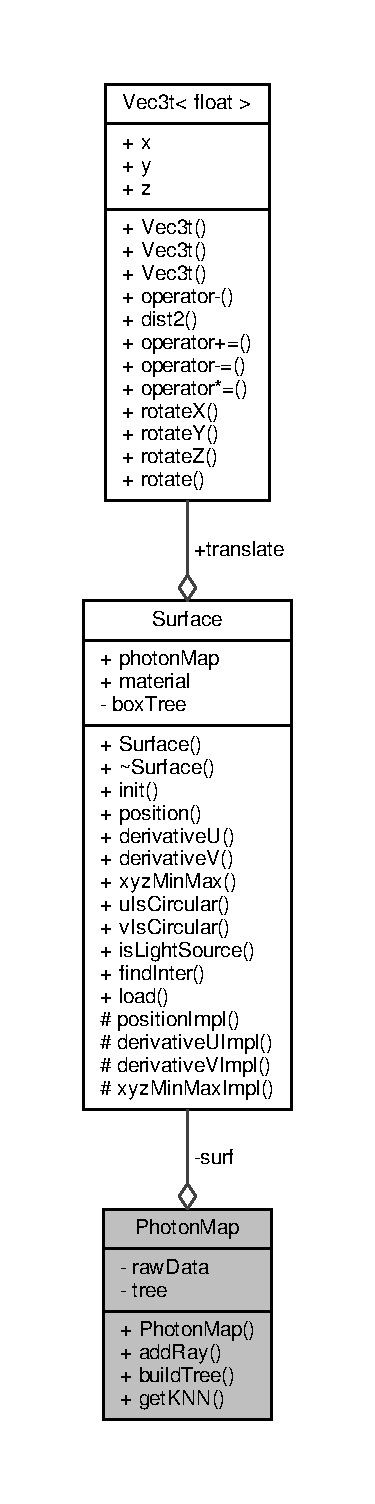
\includegraphics[height=550pt]{classPhotonMap__coll__graph}
\end{center}
\end{figure}
\subsection*{Public Member Functions}
\begin{DoxyCompactItemize}
\item 
\hyperlink{classPhotonMap_ac493f8c1f27901b6a3d5703097379332}{Photon\+Map} (const \hyperlink{classSurface}{Surface} \&\+\_\+surf)
\item 
void \hyperlink{classPhotonMap_a48205afd792b0339ed4639f2028a3145}{add\+Ray} (const \hyperlink{structColoredRay}{Colored\+Ray} \&ray)
\item 
void \hyperlink{classPhotonMap_a0a190c6a8b5dbddc76a369d022685481}{build\+Tree} ()
\item 
std\+::vector$<$ \hyperlink{structColoredRay}{Colored\+Ray} $>$ \hyperlink{classPhotonMap_a435d846181e4deed73481e49e8508c07}{get\+K\+NN} (const \hyperlink{vec_8h_ae4fcaa7c0a3935930ed1be5f70b90373}{Vec3} \&center, int k) const 
\end{DoxyCompactItemize}
\subsection*{Private Attributes}
\begin{DoxyCompactItemize}
\item 
const \hyperlink{classSurface}{Surface} \& \hyperlink{classPhotonMap_a347cfa86f86fd505194780438f1fb1d8}{surf}
\item 
std\+::unique\+\_\+ptr$<$ std\+::vector$<$ \hyperlink{structColoredRay}{Colored\+Ray} $>$ $>$ \hyperlink{classPhotonMap_a20419eecb0781c24cbda8210bc0df221}{raw\+Data}
\item 
std\+::unique\+\_\+ptr$<$ \hyperlink{classKDTree}{K\+D\+Tree} $>$ \hyperlink{classPhotonMap_aab0b914c435f74e2ce85fab273d94030}{tree}
\end{DoxyCompactItemize}


\subsection{Detailed Description}
Photon Map Use in order\+: 1. 

Add multiple rays
\begin{DoxyEnumerate}
\item Build tree
\item Find K\+NN multiple times 
\end{DoxyEnumerate}

\subsection{Constructor \& Destructor Documentation}
\index{Photon\+Map@{Photon\+Map}!Photon\+Map@{Photon\+Map}}
\index{Photon\+Map@{Photon\+Map}!Photon\+Map@{Photon\+Map}}
\subsubsection[{\texorpdfstring{Photon\+Map(const Surface \&\+\_\+surf)}{PhotonMap(const Surface &_surf)}}]{\setlength{\rightskip}{0pt plus 5cm}Photon\+Map\+::\+Photon\+Map (
\begin{DoxyParamCaption}
\item[{const {\bf Surface} \&}]{\+\_\+surf}
\end{DoxyParamCaption}
)}\hypertarget{classPhotonMap_ac493f8c1f27901b6a3d5703097379332}{}\label{classPhotonMap_ac493f8c1f27901b6a3d5703097379332}


\subsection{Member Function Documentation}
\index{Photon\+Map@{Photon\+Map}!add\+Ray@{add\+Ray}}
\index{add\+Ray@{add\+Ray}!Photon\+Map@{Photon\+Map}}
\subsubsection[{\texorpdfstring{add\+Ray(const Colored\+Ray \&ray)}{addRay(const ColoredRay &ray)}}]{\setlength{\rightskip}{0pt plus 5cm}void Photon\+Map\+::add\+Ray (
\begin{DoxyParamCaption}
\item[{const {\bf Colored\+Ray} \&}]{ray}
\end{DoxyParamCaption}
)\hspace{0.3cm}{\ttfamily [inline]}}\hypertarget{classPhotonMap_a48205afd792b0339ed4639f2028a3145}{}\label{classPhotonMap_a48205afd792b0339ed4639f2028a3145}
\index{Photon\+Map@{Photon\+Map}!build\+Tree@{build\+Tree}}
\index{build\+Tree@{build\+Tree}!Photon\+Map@{Photon\+Map}}
\subsubsection[{\texorpdfstring{build\+Tree()}{buildTree()}}]{\setlength{\rightskip}{0pt plus 5cm}void Photon\+Map\+::build\+Tree (
\begin{DoxyParamCaption}
{}
\end{DoxyParamCaption}
)}\hypertarget{classPhotonMap_a0a190c6a8b5dbddc76a369d022685481}{}\label{classPhotonMap_a0a190c6a8b5dbddc76a369d022685481}
\index{Photon\+Map@{Photon\+Map}!get\+K\+NN@{get\+K\+NN}}
\index{get\+K\+NN@{get\+K\+NN}!Photon\+Map@{Photon\+Map}}
\subsubsection[{\texorpdfstring{get\+K\+N\+N(const Vec3 \&center, int k) const }{getKNN(const Vec3 &center, int k) const }}]{\setlength{\rightskip}{0pt plus 5cm}std\+::vector$<$ {\bf Colored\+Ray} $>$ Photon\+Map\+::get\+K\+NN (
\begin{DoxyParamCaption}
\item[{const {\bf Vec3} \&}]{center, }
\item[{int}]{k}
\end{DoxyParamCaption}
) const}\hypertarget{classPhotonMap_a435d846181e4deed73481e49e8508c07}{}\label{classPhotonMap_a435d846181e4deed73481e49e8508c07}


\subsection{Member Data Documentation}
\index{Photon\+Map@{Photon\+Map}!raw\+Data@{raw\+Data}}
\index{raw\+Data@{raw\+Data}!Photon\+Map@{Photon\+Map}}
\subsubsection[{\texorpdfstring{raw\+Data}{rawData}}]{\setlength{\rightskip}{0pt plus 5cm}std\+::unique\+\_\+ptr$<$ std\+::vector$<${\bf Colored\+Ray}$>$ $>$ Photon\+Map\+::raw\+Data\hspace{0.3cm}{\ttfamily [private]}}\hypertarget{classPhotonMap_a20419eecb0781c24cbda8210bc0df221}{}\label{classPhotonMap_a20419eecb0781c24cbda8210bc0df221}
\index{Photon\+Map@{Photon\+Map}!surf@{surf}}
\index{surf@{surf}!Photon\+Map@{Photon\+Map}}
\subsubsection[{\texorpdfstring{surf}{surf}}]{\setlength{\rightskip}{0pt plus 5cm}const {\bf Surface}\& Photon\+Map\+::surf\hspace{0.3cm}{\ttfamily [private]}}\hypertarget{classPhotonMap_a347cfa86f86fd505194780438f1fb1d8}{}\label{classPhotonMap_a347cfa86f86fd505194780438f1fb1d8}
\index{Photon\+Map@{Photon\+Map}!tree@{tree}}
\index{tree@{tree}!Photon\+Map@{Photon\+Map}}
\subsubsection[{\texorpdfstring{tree}{tree}}]{\setlength{\rightskip}{0pt plus 5cm}std\+::unique\+\_\+ptr$<${\bf K\+D\+Tree}$>$ Photon\+Map\+::tree\hspace{0.3cm}{\ttfamily [private]}}\hypertarget{classPhotonMap_aab0b914c435f74e2ce85fab273d94030}{}\label{classPhotonMap_aab0b914c435f74e2ce85fab273d94030}


The documentation for this class was generated from the following files\+:\begin{DoxyCompactItemize}
\item 
\hyperlink{photonmap_8h}{photonmap.\+h}\item 
\hyperlink{photonmap_8cpp}{photonmap.\+cpp}\end{DoxyCompactItemize}

\hypertarget{structRay}{}\section{Ray Struct Reference}
\label{structRay}\index{Ray@{Ray}}


{\ttfamily \#include $<$ray.\+h$>$}



Collaboration diagram for Ray\+:
\nopagebreak
\begin{figure}[H]
\begin{center}
\leavevmode
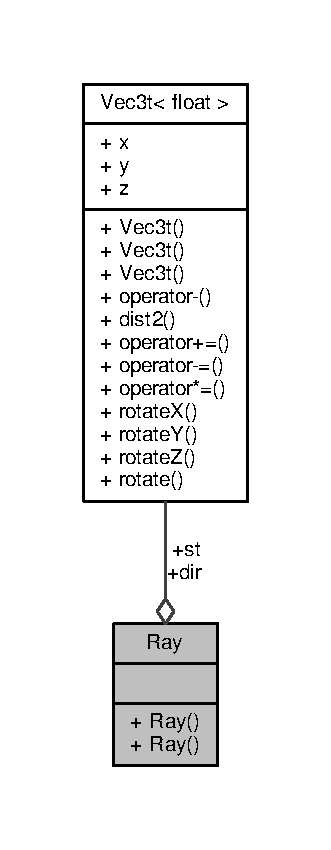
\includegraphics[width=159pt]{structRay__coll__graph}
\end{center}
\end{figure}
\subsection*{Public Member Functions}
\begin{DoxyCompactItemize}
\item 
\hyperlink{structRay_a2e3d2c29f2df4ab3da10da79d4acb852}{Ray} ()
\begin{DoxyCompactList}\small\item\em Direction. \end{DoxyCompactList}\item 
\hyperlink{structRay_a8cf3788de5062520f18684918b0347d8}{Ray} (const \hyperlink{vec_8h_ae4fcaa7c0a3935930ed1be5f70b90373}{Vec3} \&\+\_\+st, const \hyperlink{vec_8h_ae4fcaa7c0a3935930ed1be5f70b90373}{Vec3} \&\+\_\+dir)
\end{DoxyCompactItemize}
\subsection*{Public Attributes}
\begin{DoxyCompactItemize}
\item 
\hyperlink{vec_8h_ae4fcaa7c0a3935930ed1be5f70b90373}{Vec3} \hyperlink{structRay_a74977b46b5c58c6dd7b0bd90f7220309}{st}
\item 
\hyperlink{vec_8h_ae4fcaa7c0a3935930ed1be5f70b90373}{Vec3} \hyperlink{structRay_aea46150e156c321ab3162d4fb0d11668}{dir}
\begin{DoxyCompactList}\small\item\em Starting point. \end{DoxyCompactList}\end{DoxyCompactItemize}


\subsection{Constructor \& Destructor Documentation}
\index{Ray@{Ray}!Ray@{Ray}}
\index{Ray@{Ray}!Ray@{Ray}}
\subsubsection[{\texorpdfstring{Ray()}{Ray()}}]{\setlength{\rightskip}{0pt plus 5cm}Ray\+::\+Ray (
\begin{DoxyParamCaption}
{}
\end{DoxyParamCaption}
)\hspace{0.3cm}{\ttfamily [inline]}}\hypertarget{structRay_a2e3d2c29f2df4ab3da10da79d4acb852}{}\label{structRay_a2e3d2c29f2df4ab3da10da79d4acb852}


Direction. 

\index{Ray@{Ray}!Ray@{Ray}}
\index{Ray@{Ray}!Ray@{Ray}}
\subsubsection[{\texorpdfstring{Ray(const Vec3 \&\+\_\+st, const Vec3 \&\+\_\+dir)}{Ray(const Vec3 &_st, const Vec3 &_dir)}}]{\setlength{\rightskip}{0pt plus 5cm}Ray\+::\+Ray (
\begin{DoxyParamCaption}
\item[{const {\bf Vec3} \&}]{\+\_\+st, }
\item[{const {\bf Vec3} \&}]{\+\_\+dir}
\end{DoxyParamCaption}
)\hspace{0.3cm}{\ttfamily [inline]}}\hypertarget{structRay_a8cf3788de5062520f18684918b0347d8}{}\label{structRay_a8cf3788de5062520f18684918b0347d8}


\subsection{Member Data Documentation}
\index{Ray@{Ray}!dir@{dir}}
\index{dir@{dir}!Ray@{Ray}}
\subsubsection[{\texorpdfstring{dir}{dir}}]{\setlength{\rightskip}{0pt plus 5cm}{\bf Vec3} Ray\+::dir}\hypertarget{structRay_aea46150e156c321ab3162d4fb0d11668}{}\label{structRay_aea46150e156c321ab3162d4fb0d11668}


Starting point. 

\index{Ray@{Ray}!st@{st}}
\index{st@{st}!Ray@{Ray}}
\subsubsection[{\texorpdfstring{st}{st}}]{\setlength{\rightskip}{0pt plus 5cm}{\bf Vec3} Ray\+::st}\hypertarget{structRay_a74977b46b5c58c6dd7b0bd90f7220309}{}\label{structRay_a74977b46b5c58c6dd7b0bd90f7220309}


The documentation for this struct was generated from the following file\+:\begin{DoxyCompactItemize}
\item 
\hyperlink{ray_8h}{ray.\+h}\end{DoxyCompactItemize}

\hypertarget{classSquareXY}{}\section{Square\+XY Class Reference}
\label{classSquareXY}\index{Square\+XY@{Square\+XY}}


Square on x-\/y plane Upwards means outwards.  




{\ttfamily \#include $<$squarexy.\+h$>$}



Inheritance diagram for Square\+XY\+:\nopagebreak
\begin{figure}[H]
\begin{center}
\leavevmode
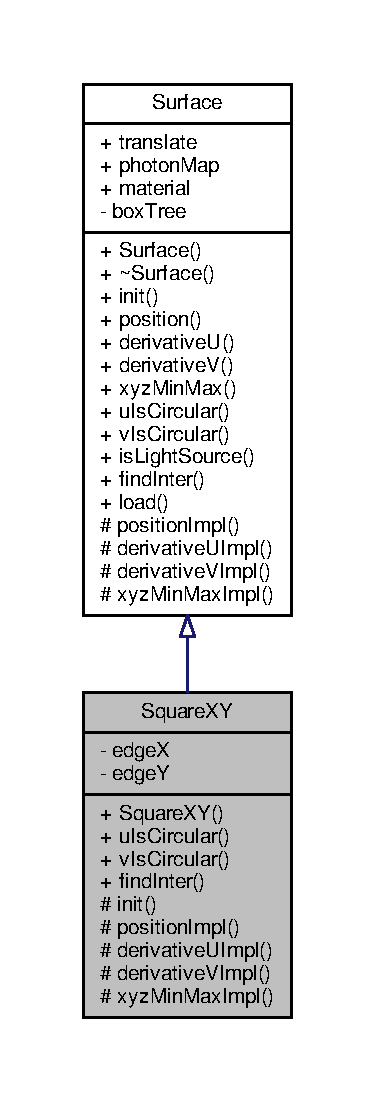
\includegraphics[width=180pt]{classSquareXY__inherit__graph}
\end{center}
\end{figure}


Collaboration diagram for Square\+XY\+:\nopagebreak
\begin{figure}[H]
\begin{center}
\leavevmode
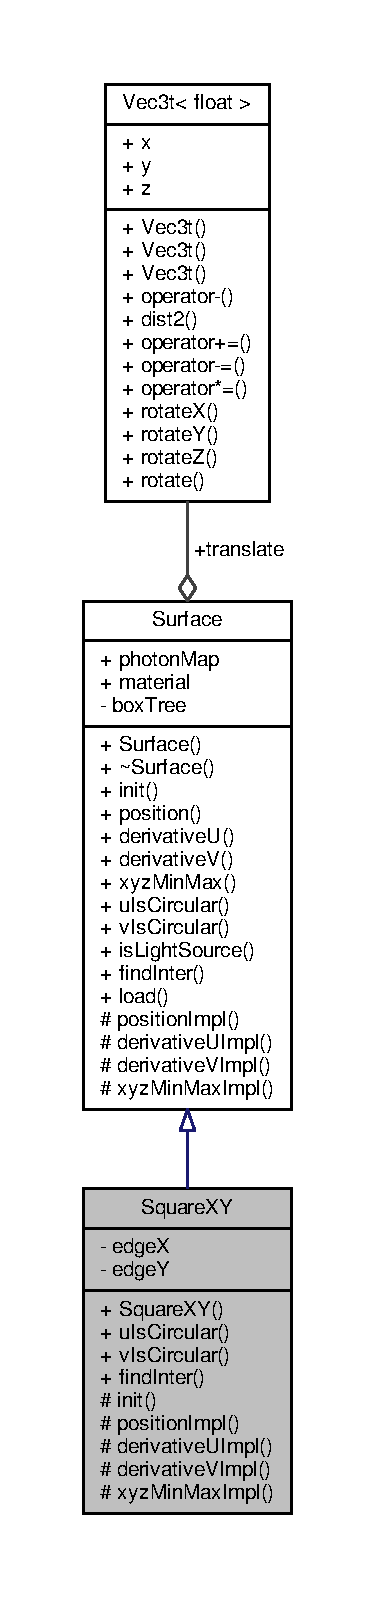
\includegraphics[height=550pt]{classSquareXY__coll__graph}
\end{center}
\end{figure}
\subsection*{Public Member Functions}
\begin{DoxyCompactItemize}
\item 
\hyperlink{classSquareXY_abeafd51f0c01d2c479f0d87ccb66567e}{Square\+XY} (float \+\_\+edgeX, float \+\_\+edgeY)
\item 
bool \hyperlink{classSquareXY_a060cba6cee229bbe185bd59fbc49c461}{u\+Is\+Circular} () const override
\item 
bool \hyperlink{classSquareXY_aeebe33da47d345225afba03b8aa110dc}{v\+Is\+Circular} () const override
\item 
\hyperlink{classOptional}{Optional}$<$ \hyperlink{structSurfInterType}{Surf\+Inter\+Type} $>$ \hyperlink{classSquareXY_a33545d952933da0107ca9d9a6c8301ff}{find\+Inter} (const \hyperlink{structRay}{Ray} \&ray) const override
\begin{DoxyCompactList}\small\item\em Find intersection on 1 surface. \end{DoxyCompactList}\end{DoxyCompactItemize}
\subsection*{Protected Member Functions}
\begin{DoxyCompactItemize}
\item 
void \hyperlink{classSquareXY_a9dfeebdb190f64c6085625e2dcf7d400}{init} () override
\begin{DoxyCompactList}\small\item\em Something can\textquotesingle{}t be put in constructor. \end{DoxyCompactList}\item 
\hyperlink{vec_8h_ae4fcaa7c0a3935930ed1be5f70b90373}{Vec3} \hyperlink{classSquareXY_a3d47992c4b73c6f49bade1c7e3fe05fe}{position\+Impl} (float u, float v) const override
\begin{DoxyCompactList}\small\item\em Do nothing because find\+Inter is overrided. \end{DoxyCompactList}\item 
\hyperlink{vec_8h_ae4fcaa7c0a3935930ed1be5f70b90373}{Vec3} \hyperlink{classSquareXY_a7507f187a31f589c06afe6dbcbccfe46}{derivative\+U\+Impl} (float u, float v) const override
\item 
\hyperlink{vec_8h_ae4fcaa7c0a3935930ed1be5f70b90373}{Vec3} \hyperlink{classSquareXY_a4803259cb98c12ba97eb9e8c57463b2d}{derivative\+V\+Impl} (float u, float v) const override
\item 
\hyperlink{structBox3}{Box3} \hyperlink{classSquareXY_ae03eb06fd6a8b493ebd1acbb0d22f365}{xyz\+Min\+Max\+Impl} (float u1, float u2, float v1, float v2) const override
\end{DoxyCompactItemize}
\subsection*{Private Attributes}
\begin{DoxyCompactItemize}
\item 
float \hyperlink{classSquareXY_abf2008e382a25547045a77c15339d465}{edgeX}
\item 
float \hyperlink{classSquareXY_a6ebaa2b3dffa23795ea2e887b3e5e0c1}{edgeY}
\end{DoxyCompactItemize}
\subsection*{Additional Inherited Members}


\subsection{Detailed Description}
Square on x-\/y plane Upwards means outwards. 

\subsection{Constructor \& Destructor Documentation}
\index{Square\+XY@{Square\+XY}!Square\+XY@{Square\+XY}}
\index{Square\+XY@{Square\+XY}!Square\+XY@{Square\+XY}}
\subsubsection[{\texorpdfstring{Square\+X\+Y(float \+\_\+edge\+X, float \+\_\+edge\+Y)}{SquareXY(float _edgeX, float _edgeY)}}]{\setlength{\rightskip}{0pt plus 5cm}Square\+X\+Y\+::\+Square\+XY (
\begin{DoxyParamCaption}
\item[{float}]{\+\_\+edgeX, }
\item[{float}]{\+\_\+edgeY}
\end{DoxyParamCaption}
)\hspace{0.3cm}{\ttfamily [inline]}}\hypertarget{classSquareXY_abeafd51f0c01d2c479f0d87ccb66567e}{}\label{classSquareXY_abeafd51f0c01d2c479f0d87ccb66567e}


\subsection{Member Function Documentation}
\index{Square\+XY@{Square\+XY}!derivative\+U\+Impl@{derivative\+U\+Impl}}
\index{derivative\+U\+Impl@{derivative\+U\+Impl}!Square\+XY@{Square\+XY}}
\subsubsection[{\texorpdfstring{derivative\+U\+Impl(float u, float v) const override}{derivativeUImpl(float u, float v) const override}}]{\setlength{\rightskip}{0pt plus 5cm}{\bf Vec3} Square\+X\+Y\+::derivative\+U\+Impl (
\begin{DoxyParamCaption}
\item[{float}]{u, }
\item[{float}]{v}
\end{DoxyParamCaption}
) const\hspace{0.3cm}{\ttfamily [inline]}, {\ttfamily [override]}, {\ttfamily [protected]}, {\ttfamily [virtual]}}\hypertarget{classSquareXY_a7507f187a31f589c06afe6dbcbccfe46}{}\label{classSquareXY_a7507f187a31f589c06afe6dbcbccfe46}


Implements \hyperlink{classSurface_a4de8fb9d4652cc32022c95eb903cce4a}{Surface}.

\index{Square\+XY@{Square\+XY}!derivative\+V\+Impl@{derivative\+V\+Impl}}
\index{derivative\+V\+Impl@{derivative\+V\+Impl}!Square\+XY@{Square\+XY}}
\subsubsection[{\texorpdfstring{derivative\+V\+Impl(float u, float v) const override}{derivativeVImpl(float u, float v) const override}}]{\setlength{\rightskip}{0pt plus 5cm}{\bf Vec3} Square\+X\+Y\+::derivative\+V\+Impl (
\begin{DoxyParamCaption}
\item[{float}]{u, }
\item[{float}]{v}
\end{DoxyParamCaption}
) const\hspace{0.3cm}{\ttfamily [inline]}, {\ttfamily [override]}, {\ttfamily [protected]}, {\ttfamily [virtual]}}\hypertarget{classSquareXY_a4803259cb98c12ba97eb9e8c57463b2d}{}\label{classSquareXY_a4803259cb98c12ba97eb9e8c57463b2d}


Implements \hyperlink{classSurface_a95d65437419ba8d439fa8f0d71f963a1}{Surface}.

\index{Square\+XY@{Square\+XY}!find\+Inter@{find\+Inter}}
\index{find\+Inter@{find\+Inter}!Square\+XY@{Square\+XY}}
\subsubsection[{\texorpdfstring{find\+Inter(const Ray \&ray) const override}{findInter(const Ray &ray) const override}}]{\setlength{\rightskip}{0pt plus 5cm}{\bf Optional}$<${\bf Surf\+Inter\+Type}$>$ Square\+X\+Y\+::find\+Inter (
\begin{DoxyParamCaption}
\item[{const {\bf Ray} \&}]{ray}
\end{DoxyParamCaption}
) const\hspace{0.3cm}{\ttfamily [inline]}, {\ttfamily [override]}, {\ttfamily [virtual]}}\hypertarget{classSquareXY_a33545d952933da0107ca9d9a6c8301ff}{}\label{classSquareXY_a33545d952933da0107ca9d9a6c8301ff}


Find intersection on 1 surface. 



Reimplemented from \hyperlink{classSurface_af7b5584007bf626bf7b37fcf649e6cd6}{Surface}.

\index{Square\+XY@{Square\+XY}!init@{init}}
\index{init@{init}!Square\+XY@{Square\+XY}}
\subsubsection[{\texorpdfstring{init() override}{init() override}}]{\setlength{\rightskip}{0pt plus 5cm}void Square\+X\+Y\+::init (
\begin{DoxyParamCaption}
{}
\end{DoxyParamCaption}
)\hspace{0.3cm}{\ttfamily [inline]}, {\ttfamily [override]}, {\ttfamily [protected]}, {\ttfamily [virtual]}}\hypertarget{classSquareXY_a9dfeebdb190f64c6085625e2dcf7d400}{}\label{classSquareXY_a9dfeebdb190f64c6085625e2dcf7d400}


Something can\textquotesingle{}t be put in constructor. 



Reimplemented from \hyperlink{classSurface_a194087202684a4b3a71c24f02faeb404}{Surface}.

\index{Square\+XY@{Square\+XY}!position\+Impl@{position\+Impl}}
\index{position\+Impl@{position\+Impl}!Square\+XY@{Square\+XY}}
\subsubsection[{\texorpdfstring{position\+Impl(float u, float v) const override}{positionImpl(float u, float v) const override}}]{\setlength{\rightskip}{0pt plus 5cm}{\bf Vec3} Square\+X\+Y\+::position\+Impl (
\begin{DoxyParamCaption}
\item[{float}]{u, }
\item[{float}]{v}
\end{DoxyParamCaption}
) const\hspace{0.3cm}{\ttfamily [inline]}, {\ttfamily [override]}, {\ttfamily [protected]}, {\ttfamily [virtual]}}\hypertarget{classSquareXY_a3d47992c4b73c6f49bade1c7e3fe05fe}{}\label{classSquareXY_a3d47992c4b73c6f49bade1c7e3fe05fe}


Do nothing because find\+Inter is overrided. 



Implements \hyperlink{classSurface_a379545eea4809f81fe7e037f5e5ff4be}{Surface}.

\index{Square\+XY@{Square\+XY}!u\+Is\+Circular@{u\+Is\+Circular}}
\index{u\+Is\+Circular@{u\+Is\+Circular}!Square\+XY@{Square\+XY}}
\subsubsection[{\texorpdfstring{u\+Is\+Circular() const override}{uIsCircular() const override}}]{\setlength{\rightskip}{0pt plus 5cm}bool Square\+X\+Y\+::u\+Is\+Circular (
\begin{DoxyParamCaption}
{}
\end{DoxyParamCaption}
) const\hspace{0.3cm}{\ttfamily [inline]}, {\ttfamily [override]}, {\ttfamily [virtual]}}\hypertarget{classSquareXY_a060cba6cee229bbe185bd59fbc49c461}{}\label{classSquareXY_a060cba6cee229bbe185bd59fbc49c461}


Implements \hyperlink{classSurface_a11d5759ec3e3d43036fb949dcc6f5562}{Surface}.

\index{Square\+XY@{Square\+XY}!v\+Is\+Circular@{v\+Is\+Circular}}
\index{v\+Is\+Circular@{v\+Is\+Circular}!Square\+XY@{Square\+XY}}
\subsubsection[{\texorpdfstring{v\+Is\+Circular() const override}{vIsCircular() const override}}]{\setlength{\rightskip}{0pt plus 5cm}bool Square\+X\+Y\+::v\+Is\+Circular (
\begin{DoxyParamCaption}
{}
\end{DoxyParamCaption}
) const\hspace{0.3cm}{\ttfamily [inline]}, {\ttfamily [override]}, {\ttfamily [virtual]}}\hypertarget{classSquareXY_aeebe33da47d345225afba03b8aa110dc}{}\label{classSquareXY_aeebe33da47d345225afba03b8aa110dc}


Implements \hyperlink{classSurface_af52f9322929a702a9aaeee3ae4a368da}{Surface}.

\index{Square\+XY@{Square\+XY}!xyz\+Min\+Max\+Impl@{xyz\+Min\+Max\+Impl}}
\index{xyz\+Min\+Max\+Impl@{xyz\+Min\+Max\+Impl}!Square\+XY@{Square\+XY}}
\subsubsection[{\texorpdfstring{xyz\+Min\+Max\+Impl(float u1, float u2, float v1, float v2) const override}{xyzMinMaxImpl(float u1, float u2, float v1, float v2) const override}}]{\setlength{\rightskip}{0pt plus 5cm}{\bf Box3} Square\+X\+Y\+::xyz\+Min\+Max\+Impl (
\begin{DoxyParamCaption}
\item[{float}]{u1, }
\item[{float}]{u2, }
\item[{float}]{v1, }
\item[{float}]{v2}
\end{DoxyParamCaption}
) const\hspace{0.3cm}{\ttfamily [inline]}, {\ttfamily [override]}, {\ttfamily [protected]}, {\ttfamily [virtual]}}\hypertarget{classSquareXY_ae03eb06fd6a8b493ebd1acbb0d22f365}{}\label{classSquareXY_ae03eb06fd6a8b493ebd1acbb0d22f365}


Implements \hyperlink{classSurface_ab1ee990da290748cd86aaf95edb28c38}{Surface}.



\subsection{Member Data Documentation}
\index{Square\+XY@{Square\+XY}!edgeX@{edgeX}}
\index{edgeX@{edgeX}!Square\+XY@{Square\+XY}}
\subsubsection[{\texorpdfstring{edgeX}{edgeX}}]{\setlength{\rightskip}{0pt plus 5cm}float Square\+X\+Y\+::edgeX\hspace{0.3cm}{\ttfamily [private]}}\hypertarget{classSquareXY_abf2008e382a25547045a77c15339d465}{}\label{classSquareXY_abf2008e382a25547045a77c15339d465}
\index{Square\+XY@{Square\+XY}!edgeY@{edgeY}}
\index{edgeY@{edgeY}!Square\+XY@{Square\+XY}}
\subsubsection[{\texorpdfstring{edgeY}{edgeY}}]{\setlength{\rightskip}{0pt plus 5cm}float Square\+X\+Y\+::edgeY\hspace{0.3cm}{\ttfamily [private]}}\hypertarget{classSquareXY_a6ebaa2b3dffa23795ea2e887b3e5e0c1}{}\label{classSquareXY_a6ebaa2b3dffa23795ea2e887b3e5e0c1}


The documentation for this class was generated from the following file\+:\begin{DoxyCompactItemize}
\item 
\hyperlink{squarexy_8h}{squarexy.\+h}\end{DoxyCompactItemize}

\hypertarget{classSquareYZ}{}\section{Square\+YZ Class Reference}
\label{classSquareYZ}\index{Square\+YZ@{Square\+YZ}}


Square on y-\/z plane x+ means outwards.  




{\ttfamily \#include $<$squareyz.\+h$>$}



Inheritance diagram for Square\+YZ\+:\nopagebreak
\begin{figure}[H]
\begin{center}
\leavevmode
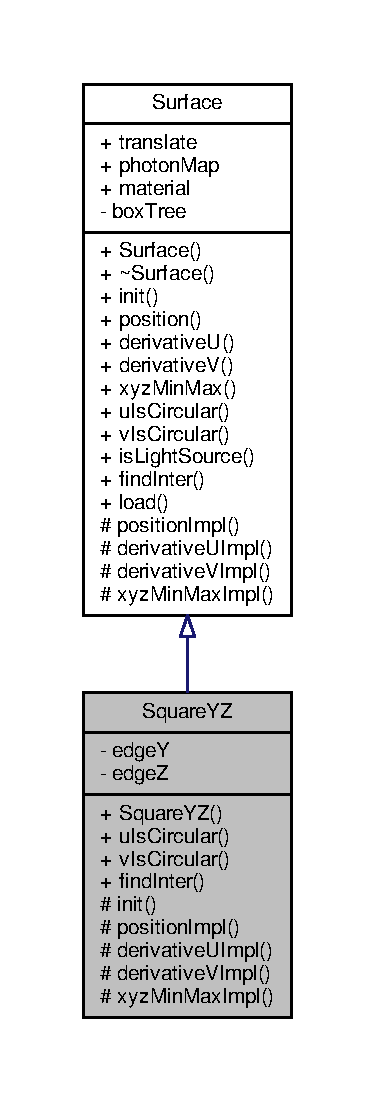
\includegraphics[width=180pt]{classSquareYZ__inherit__graph}
\end{center}
\end{figure}


Collaboration diagram for Square\+YZ\+:\nopagebreak
\begin{figure}[H]
\begin{center}
\leavevmode
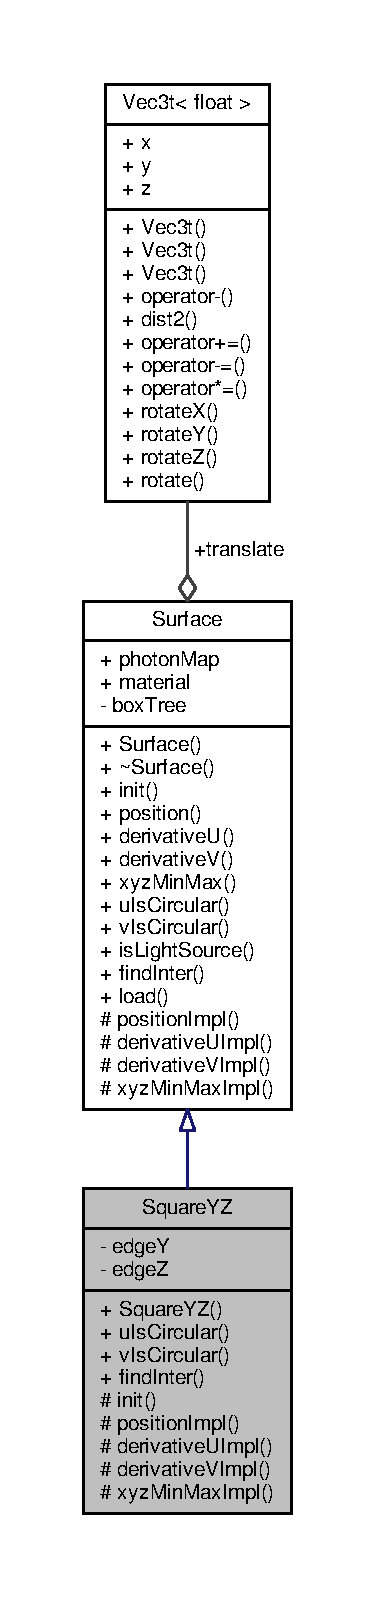
\includegraphics[height=550pt]{classSquareYZ__coll__graph}
\end{center}
\end{figure}
\subsection*{Public Member Functions}
\begin{DoxyCompactItemize}
\item 
\hyperlink{classSquareYZ_a3d88bfd27f8d9a833a54ef3d2d885831}{Square\+YZ} (float \+\_\+edgeY, float \+\_\+edgeZ)
\item 
bool \hyperlink{classSquareYZ_adc74593250e7aaf7f8d733e22e3951b6}{u\+Is\+Circular} () const override
\item 
bool \hyperlink{classSquareYZ_ab6a94e65acedccedd4556023b1490841}{v\+Is\+Circular} () const override
\item 
\hyperlink{classOptional}{Optional}$<$ \hyperlink{structSurfInterType}{Surf\+Inter\+Type} $>$ \hyperlink{classSquareYZ_a75ffd1eda4c026706513dfa07043ffc8}{find\+Inter} (const \hyperlink{structRay}{Ray} \&ray) const override
\begin{DoxyCompactList}\small\item\em Find intersection on 1 surface. \end{DoxyCompactList}\end{DoxyCompactItemize}
\subsection*{Protected Member Functions}
\begin{DoxyCompactItemize}
\item 
void \hyperlink{classSquareYZ_a1d82d4fea479dd58096d723eb9109cfe}{init} () override
\begin{DoxyCompactList}\small\item\em Something can\textquotesingle{}t be put in constructor. \end{DoxyCompactList}\item 
\hyperlink{vec_8h_ae4fcaa7c0a3935930ed1be5f70b90373}{Vec3} \hyperlink{classSquareYZ_a56695f7f1cbd288bf93918deac0feb4c}{position\+Impl} (float u, float v) const override
\begin{DoxyCompactList}\small\item\em Do nothing because find\+Inter is overrided. \end{DoxyCompactList}\item 
\hyperlink{vec_8h_ae4fcaa7c0a3935930ed1be5f70b90373}{Vec3} \hyperlink{classSquareYZ_a2b37c54c61d5f2896657f8510884e64e}{derivative\+U\+Impl} (float u, float v) const override
\item 
\hyperlink{vec_8h_ae4fcaa7c0a3935930ed1be5f70b90373}{Vec3} \hyperlink{classSquareYZ_a6fc7a2189bf889b0dd99c229d2a6d0da}{derivative\+V\+Impl} (float u, float v) const override
\item 
\hyperlink{structBox3}{Box3} \hyperlink{classSquareYZ_a61260b3bae72f9354a8fe4c145bce87d}{xyz\+Min\+Max\+Impl} (float u1, float u2, float v1, float v2) const override
\end{DoxyCompactItemize}
\subsection*{Private Attributes}
\begin{DoxyCompactItemize}
\item 
float \hyperlink{classSquareYZ_a6d7f81cfc7814c9d3f948b0115606254}{edgeY}
\item 
float \hyperlink{classSquareYZ_a87fc6f3c129ce52756296f2cbf402bc6}{edgeZ}
\end{DoxyCompactItemize}
\subsection*{Additional Inherited Members}


\subsection{Detailed Description}
Square on y-\/z plane x+ means outwards. 

\subsection{Constructor \& Destructor Documentation}
\index{Square\+YZ@{Square\+YZ}!Square\+YZ@{Square\+YZ}}
\index{Square\+YZ@{Square\+YZ}!Square\+YZ@{Square\+YZ}}
\subsubsection[{\texorpdfstring{Square\+Y\+Z(float \+\_\+edge\+Y, float \+\_\+edge\+Z)}{SquareYZ(float _edgeY, float _edgeZ)}}]{\setlength{\rightskip}{0pt plus 5cm}Square\+Y\+Z\+::\+Square\+YZ (
\begin{DoxyParamCaption}
\item[{float}]{\+\_\+edgeY, }
\item[{float}]{\+\_\+edgeZ}
\end{DoxyParamCaption}
)\hspace{0.3cm}{\ttfamily [inline]}}\hypertarget{classSquareYZ_a3d88bfd27f8d9a833a54ef3d2d885831}{}\label{classSquareYZ_a3d88bfd27f8d9a833a54ef3d2d885831}


\subsection{Member Function Documentation}
\index{Square\+YZ@{Square\+YZ}!derivative\+U\+Impl@{derivative\+U\+Impl}}
\index{derivative\+U\+Impl@{derivative\+U\+Impl}!Square\+YZ@{Square\+YZ}}
\subsubsection[{\texorpdfstring{derivative\+U\+Impl(float u, float v) const override}{derivativeUImpl(float u, float v) const override}}]{\setlength{\rightskip}{0pt plus 5cm}{\bf Vec3} Square\+Y\+Z\+::derivative\+U\+Impl (
\begin{DoxyParamCaption}
\item[{float}]{u, }
\item[{float}]{v}
\end{DoxyParamCaption}
) const\hspace{0.3cm}{\ttfamily [inline]}, {\ttfamily [override]}, {\ttfamily [protected]}, {\ttfamily [virtual]}}\hypertarget{classSquareYZ_a2b37c54c61d5f2896657f8510884e64e}{}\label{classSquareYZ_a2b37c54c61d5f2896657f8510884e64e}


Implements \hyperlink{classSurface_a4de8fb9d4652cc32022c95eb903cce4a}{Surface}.

\index{Square\+YZ@{Square\+YZ}!derivative\+V\+Impl@{derivative\+V\+Impl}}
\index{derivative\+V\+Impl@{derivative\+V\+Impl}!Square\+YZ@{Square\+YZ}}
\subsubsection[{\texorpdfstring{derivative\+V\+Impl(float u, float v) const override}{derivativeVImpl(float u, float v) const override}}]{\setlength{\rightskip}{0pt plus 5cm}{\bf Vec3} Square\+Y\+Z\+::derivative\+V\+Impl (
\begin{DoxyParamCaption}
\item[{float}]{u, }
\item[{float}]{v}
\end{DoxyParamCaption}
) const\hspace{0.3cm}{\ttfamily [inline]}, {\ttfamily [override]}, {\ttfamily [protected]}, {\ttfamily [virtual]}}\hypertarget{classSquareYZ_a6fc7a2189bf889b0dd99c229d2a6d0da}{}\label{classSquareYZ_a6fc7a2189bf889b0dd99c229d2a6d0da}


Implements \hyperlink{classSurface_a95d65437419ba8d439fa8f0d71f963a1}{Surface}.

\index{Square\+YZ@{Square\+YZ}!find\+Inter@{find\+Inter}}
\index{find\+Inter@{find\+Inter}!Square\+YZ@{Square\+YZ}}
\subsubsection[{\texorpdfstring{find\+Inter(const Ray \&ray) const override}{findInter(const Ray &ray) const override}}]{\setlength{\rightskip}{0pt plus 5cm}{\bf Optional}$<${\bf Surf\+Inter\+Type}$>$ Square\+Y\+Z\+::find\+Inter (
\begin{DoxyParamCaption}
\item[{const {\bf Ray} \&}]{ray}
\end{DoxyParamCaption}
) const\hspace{0.3cm}{\ttfamily [inline]}, {\ttfamily [override]}, {\ttfamily [virtual]}}\hypertarget{classSquareYZ_a75ffd1eda4c026706513dfa07043ffc8}{}\label{classSquareYZ_a75ffd1eda4c026706513dfa07043ffc8}


Find intersection on 1 surface. 



Reimplemented from \hyperlink{classSurface_af7b5584007bf626bf7b37fcf649e6cd6}{Surface}.

\index{Square\+YZ@{Square\+YZ}!init@{init}}
\index{init@{init}!Square\+YZ@{Square\+YZ}}
\subsubsection[{\texorpdfstring{init() override}{init() override}}]{\setlength{\rightskip}{0pt plus 5cm}void Square\+Y\+Z\+::init (
\begin{DoxyParamCaption}
{}
\end{DoxyParamCaption}
)\hspace{0.3cm}{\ttfamily [inline]}, {\ttfamily [override]}, {\ttfamily [protected]}, {\ttfamily [virtual]}}\hypertarget{classSquareYZ_a1d82d4fea479dd58096d723eb9109cfe}{}\label{classSquareYZ_a1d82d4fea479dd58096d723eb9109cfe}


Something can\textquotesingle{}t be put in constructor. 



Reimplemented from \hyperlink{classSurface_a194087202684a4b3a71c24f02faeb404}{Surface}.

\index{Square\+YZ@{Square\+YZ}!position\+Impl@{position\+Impl}}
\index{position\+Impl@{position\+Impl}!Square\+YZ@{Square\+YZ}}
\subsubsection[{\texorpdfstring{position\+Impl(float u, float v) const override}{positionImpl(float u, float v) const override}}]{\setlength{\rightskip}{0pt plus 5cm}{\bf Vec3} Square\+Y\+Z\+::position\+Impl (
\begin{DoxyParamCaption}
\item[{float}]{u, }
\item[{float}]{v}
\end{DoxyParamCaption}
) const\hspace{0.3cm}{\ttfamily [inline]}, {\ttfamily [override]}, {\ttfamily [protected]}, {\ttfamily [virtual]}}\hypertarget{classSquareYZ_a56695f7f1cbd288bf93918deac0feb4c}{}\label{classSquareYZ_a56695f7f1cbd288bf93918deac0feb4c}


Do nothing because find\+Inter is overrided. 



Implements \hyperlink{classSurface_a379545eea4809f81fe7e037f5e5ff4be}{Surface}.

\index{Square\+YZ@{Square\+YZ}!u\+Is\+Circular@{u\+Is\+Circular}}
\index{u\+Is\+Circular@{u\+Is\+Circular}!Square\+YZ@{Square\+YZ}}
\subsubsection[{\texorpdfstring{u\+Is\+Circular() const override}{uIsCircular() const override}}]{\setlength{\rightskip}{0pt plus 5cm}bool Square\+Y\+Z\+::u\+Is\+Circular (
\begin{DoxyParamCaption}
{}
\end{DoxyParamCaption}
) const\hspace{0.3cm}{\ttfamily [inline]}, {\ttfamily [override]}, {\ttfamily [virtual]}}\hypertarget{classSquareYZ_adc74593250e7aaf7f8d733e22e3951b6}{}\label{classSquareYZ_adc74593250e7aaf7f8d733e22e3951b6}


Implements \hyperlink{classSurface_a11d5759ec3e3d43036fb949dcc6f5562}{Surface}.

\index{Square\+YZ@{Square\+YZ}!v\+Is\+Circular@{v\+Is\+Circular}}
\index{v\+Is\+Circular@{v\+Is\+Circular}!Square\+YZ@{Square\+YZ}}
\subsubsection[{\texorpdfstring{v\+Is\+Circular() const override}{vIsCircular() const override}}]{\setlength{\rightskip}{0pt plus 5cm}bool Square\+Y\+Z\+::v\+Is\+Circular (
\begin{DoxyParamCaption}
{}
\end{DoxyParamCaption}
) const\hspace{0.3cm}{\ttfamily [inline]}, {\ttfamily [override]}, {\ttfamily [virtual]}}\hypertarget{classSquareYZ_ab6a94e65acedccedd4556023b1490841}{}\label{classSquareYZ_ab6a94e65acedccedd4556023b1490841}


Implements \hyperlink{classSurface_af52f9322929a702a9aaeee3ae4a368da}{Surface}.

\index{Square\+YZ@{Square\+YZ}!xyz\+Min\+Max\+Impl@{xyz\+Min\+Max\+Impl}}
\index{xyz\+Min\+Max\+Impl@{xyz\+Min\+Max\+Impl}!Square\+YZ@{Square\+YZ}}
\subsubsection[{\texorpdfstring{xyz\+Min\+Max\+Impl(float u1, float u2, float v1, float v2) const override}{xyzMinMaxImpl(float u1, float u2, float v1, float v2) const override}}]{\setlength{\rightskip}{0pt plus 5cm}{\bf Box3} Square\+Y\+Z\+::xyz\+Min\+Max\+Impl (
\begin{DoxyParamCaption}
\item[{float}]{u1, }
\item[{float}]{u2, }
\item[{float}]{v1, }
\item[{float}]{v2}
\end{DoxyParamCaption}
) const\hspace{0.3cm}{\ttfamily [inline]}, {\ttfamily [override]}, {\ttfamily [protected]}, {\ttfamily [virtual]}}\hypertarget{classSquareYZ_a61260b3bae72f9354a8fe4c145bce87d}{}\label{classSquareYZ_a61260b3bae72f9354a8fe4c145bce87d}


Implements \hyperlink{classSurface_ab1ee990da290748cd86aaf95edb28c38}{Surface}.



\subsection{Member Data Documentation}
\index{Square\+YZ@{Square\+YZ}!edgeY@{edgeY}}
\index{edgeY@{edgeY}!Square\+YZ@{Square\+YZ}}
\subsubsection[{\texorpdfstring{edgeY}{edgeY}}]{\setlength{\rightskip}{0pt plus 5cm}float Square\+Y\+Z\+::edgeY\hspace{0.3cm}{\ttfamily [private]}}\hypertarget{classSquareYZ_a6d7f81cfc7814c9d3f948b0115606254}{}\label{classSquareYZ_a6d7f81cfc7814c9d3f948b0115606254}
\index{Square\+YZ@{Square\+YZ}!edgeZ@{edgeZ}}
\index{edgeZ@{edgeZ}!Square\+YZ@{Square\+YZ}}
\subsubsection[{\texorpdfstring{edgeZ}{edgeZ}}]{\setlength{\rightskip}{0pt plus 5cm}float Square\+Y\+Z\+::edgeZ\hspace{0.3cm}{\ttfamily [private]}}\hypertarget{classSquareYZ_a87fc6f3c129ce52756296f2cbf402bc6}{}\label{classSquareYZ_a87fc6f3c129ce52756296f2cbf402bc6}


The documentation for this class was generated from the following file\+:\begin{DoxyCompactItemize}
\item 
\hyperlink{squareyz_8h}{squareyz.\+h}\end{DoxyCompactItemize}

\hypertarget{classSquareZX}{}\section{Square\+ZX Class Reference}
\label{classSquareZX}\index{Square\+ZX@{Square\+ZX}}


Square on z-\/x plane y+ means outwards.  




{\ttfamily \#include $<$squarezx.\+h$>$}



Inheritance diagram for Square\+ZX\+:
\nopagebreak
\begin{figure}[H]
\begin{center}
\leavevmode
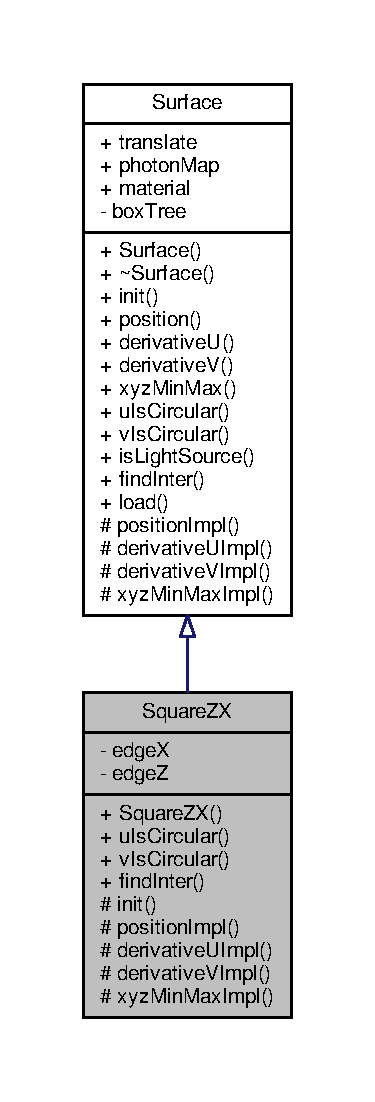
\includegraphics[width=180pt]{classSquareZX__inherit__graph}
\end{center}
\end{figure}


Collaboration diagram for Square\+ZX\+:
\nopagebreak
\begin{figure}[H]
\begin{center}
\leavevmode
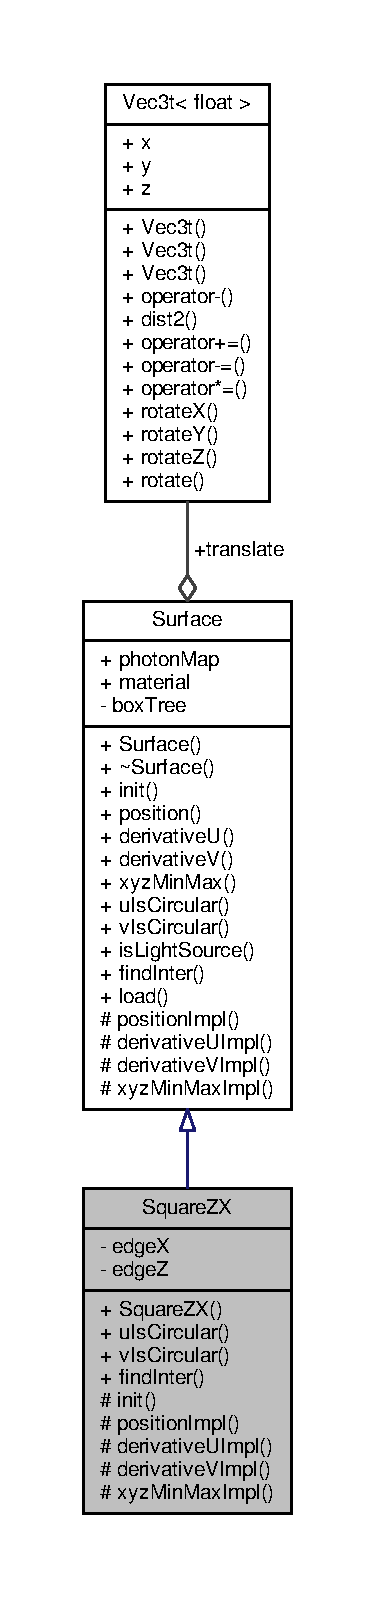
\includegraphics[height=550pt]{classSquareZX__coll__graph}
\end{center}
\end{figure}
\subsection*{Public Member Functions}
\begin{DoxyCompactItemize}
\item 
\hyperlink{classSquareZX_a18592605121c1b9f52aefd5895ee144c}{Square\+ZX} (float \+\_\+edgeX, float \+\_\+edgeZ)
\item 
bool \hyperlink{classSquareZX_a912de0928a8332afb6cb89179595668a}{u\+Is\+Circular} () const override
\item 
bool \hyperlink{classSquareZX_a5556f34a0c9e6c07f59c488857937b35}{v\+Is\+Circular} () const override
\item 
\hyperlink{classOptional}{Optional}$<$ \hyperlink{structSurfInterType}{Surf\+Inter\+Type} $>$ \hyperlink{classSquareZX_a2de50bbf52fc3243eaf1b68099224321}{find\+Inter} (const \hyperlink{structRay}{Ray} \&ray) const override
\begin{DoxyCompactList}\small\item\em Find intersection on 1 surface. \end{DoxyCompactList}\end{DoxyCompactItemize}
\subsection*{Protected Member Functions}
\begin{DoxyCompactItemize}
\item 
void \hyperlink{classSquareZX_aefbaa1f1b673aa405f427dbacc81114c}{init} () override
\begin{DoxyCompactList}\small\item\em Something can\textquotesingle{}t be put in constructor. \end{DoxyCompactList}\item 
\hyperlink{vec_8h_ae4fcaa7c0a3935930ed1be5f70b90373}{Vec3} \hyperlink{classSquareZX_a505da0c732d570991b69837e9dac89e5}{position\+Impl} (float u, float v) const override
\begin{DoxyCompactList}\small\item\em Do nothing because find\+Inter is overrided. \end{DoxyCompactList}\item 
\hyperlink{vec_8h_ae4fcaa7c0a3935930ed1be5f70b90373}{Vec3} \hyperlink{classSquareZX_aafd9b0bfc12a6034d07d4cf27b211cfd}{derivative\+U\+Impl} (float u, float v) const override
\item 
\hyperlink{vec_8h_ae4fcaa7c0a3935930ed1be5f70b90373}{Vec3} \hyperlink{classSquareZX_a3ede3591078b049a8997ad144d7f92cd}{derivative\+V\+Impl} (float u, float v) const override
\item 
\hyperlink{structBox3}{Box3} \hyperlink{classSquareZX_a87b224b775e24f1d6ba984d37d0c85eb}{xyz\+Min\+Max\+Impl} (float u1, float u2, float v1, float v2) const override
\end{DoxyCompactItemize}
\subsection*{Private Attributes}
\begin{DoxyCompactItemize}
\item 
float \hyperlink{classSquareZX_a7e460f5cda678eb9c3860303395adc8e}{edgeX}
\item 
float \hyperlink{classSquareZX_a3f05799d20b98477ea21d7479ba32e16}{edgeZ}
\end{DoxyCompactItemize}
\subsection*{Additional Inherited Members}


\subsection{Detailed Description}
Square on z-\/x plane y+ means outwards. 

\subsection{Constructor \& Destructor Documentation}
\index{Square\+ZX@{Square\+ZX}!Square\+ZX@{Square\+ZX}}
\index{Square\+ZX@{Square\+ZX}!Square\+ZX@{Square\+ZX}}
\subsubsection[{\texorpdfstring{Square\+Z\+X(float \+\_\+edge\+X, float \+\_\+edge\+Z)}{SquareZX(float _edgeX, float _edgeZ)}}]{\setlength{\rightskip}{0pt plus 5cm}Square\+Z\+X\+::\+Square\+ZX (
\begin{DoxyParamCaption}
\item[{float}]{\+\_\+edgeX, }
\item[{float}]{\+\_\+edgeZ}
\end{DoxyParamCaption}
)\hspace{0.3cm}{\ttfamily [inline]}}\hypertarget{classSquareZX_a18592605121c1b9f52aefd5895ee144c}{}\label{classSquareZX_a18592605121c1b9f52aefd5895ee144c}


\subsection{Member Function Documentation}
\index{Square\+ZX@{Square\+ZX}!derivative\+U\+Impl@{derivative\+U\+Impl}}
\index{derivative\+U\+Impl@{derivative\+U\+Impl}!Square\+ZX@{Square\+ZX}}
\subsubsection[{\texorpdfstring{derivative\+U\+Impl(float u, float v) const override}{derivativeUImpl(float u, float v) const override}}]{\setlength{\rightskip}{0pt plus 5cm}{\bf Vec3} Square\+Z\+X\+::derivative\+U\+Impl (
\begin{DoxyParamCaption}
\item[{float}]{u, }
\item[{float}]{v}
\end{DoxyParamCaption}
) const\hspace{0.3cm}{\ttfamily [inline]}, {\ttfamily [override]}, {\ttfamily [protected]}, {\ttfamily [virtual]}}\hypertarget{classSquareZX_aafd9b0bfc12a6034d07d4cf27b211cfd}{}\label{classSquareZX_aafd9b0bfc12a6034d07d4cf27b211cfd}


Implements \hyperlink{classSurface_a4de8fb9d4652cc32022c95eb903cce4a}{Surface}.

\index{Square\+ZX@{Square\+ZX}!derivative\+V\+Impl@{derivative\+V\+Impl}}
\index{derivative\+V\+Impl@{derivative\+V\+Impl}!Square\+ZX@{Square\+ZX}}
\subsubsection[{\texorpdfstring{derivative\+V\+Impl(float u, float v) const override}{derivativeVImpl(float u, float v) const override}}]{\setlength{\rightskip}{0pt plus 5cm}{\bf Vec3} Square\+Z\+X\+::derivative\+V\+Impl (
\begin{DoxyParamCaption}
\item[{float}]{u, }
\item[{float}]{v}
\end{DoxyParamCaption}
) const\hspace{0.3cm}{\ttfamily [inline]}, {\ttfamily [override]}, {\ttfamily [protected]}, {\ttfamily [virtual]}}\hypertarget{classSquareZX_a3ede3591078b049a8997ad144d7f92cd}{}\label{classSquareZX_a3ede3591078b049a8997ad144d7f92cd}


Implements \hyperlink{classSurface_a95d65437419ba8d439fa8f0d71f963a1}{Surface}.

\index{Square\+ZX@{Square\+ZX}!find\+Inter@{find\+Inter}}
\index{find\+Inter@{find\+Inter}!Square\+ZX@{Square\+ZX}}
\subsubsection[{\texorpdfstring{find\+Inter(const Ray \&ray) const override}{findInter(const Ray &ray) const override}}]{\setlength{\rightskip}{0pt plus 5cm}{\bf Optional}$<${\bf Surf\+Inter\+Type}$>$ Square\+Z\+X\+::find\+Inter (
\begin{DoxyParamCaption}
\item[{const {\bf Ray} \&}]{ray}
\end{DoxyParamCaption}
) const\hspace{0.3cm}{\ttfamily [inline]}, {\ttfamily [override]}, {\ttfamily [virtual]}}\hypertarget{classSquareZX_a2de50bbf52fc3243eaf1b68099224321}{}\label{classSquareZX_a2de50bbf52fc3243eaf1b68099224321}


Find intersection on 1 surface. 



Reimplemented from \hyperlink{classSurface_af7b5584007bf626bf7b37fcf649e6cd6}{Surface}.

\index{Square\+ZX@{Square\+ZX}!init@{init}}
\index{init@{init}!Square\+ZX@{Square\+ZX}}
\subsubsection[{\texorpdfstring{init() override}{init() override}}]{\setlength{\rightskip}{0pt plus 5cm}void Square\+Z\+X\+::init (
\begin{DoxyParamCaption}
{}
\end{DoxyParamCaption}
)\hspace{0.3cm}{\ttfamily [inline]}, {\ttfamily [override]}, {\ttfamily [protected]}, {\ttfamily [virtual]}}\hypertarget{classSquareZX_aefbaa1f1b673aa405f427dbacc81114c}{}\label{classSquareZX_aefbaa1f1b673aa405f427dbacc81114c}


Something can\textquotesingle{}t be put in constructor. 



Reimplemented from \hyperlink{classSurface_a194087202684a4b3a71c24f02faeb404}{Surface}.

\index{Square\+ZX@{Square\+ZX}!position\+Impl@{position\+Impl}}
\index{position\+Impl@{position\+Impl}!Square\+ZX@{Square\+ZX}}
\subsubsection[{\texorpdfstring{position\+Impl(float u, float v) const override}{positionImpl(float u, float v) const override}}]{\setlength{\rightskip}{0pt plus 5cm}{\bf Vec3} Square\+Z\+X\+::position\+Impl (
\begin{DoxyParamCaption}
\item[{float}]{u, }
\item[{float}]{v}
\end{DoxyParamCaption}
) const\hspace{0.3cm}{\ttfamily [inline]}, {\ttfamily [override]}, {\ttfamily [protected]}, {\ttfamily [virtual]}}\hypertarget{classSquareZX_a505da0c732d570991b69837e9dac89e5}{}\label{classSquareZX_a505da0c732d570991b69837e9dac89e5}


Do nothing because find\+Inter is overrided. 



Implements \hyperlink{classSurface_a379545eea4809f81fe7e037f5e5ff4be}{Surface}.

\index{Square\+ZX@{Square\+ZX}!u\+Is\+Circular@{u\+Is\+Circular}}
\index{u\+Is\+Circular@{u\+Is\+Circular}!Square\+ZX@{Square\+ZX}}
\subsubsection[{\texorpdfstring{u\+Is\+Circular() const override}{uIsCircular() const override}}]{\setlength{\rightskip}{0pt plus 5cm}bool Square\+Z\+X\+::u\+Is\+Circular (
\begin{DoxyParamCaption}
{}
\end{DoxyParamCaption}
) const\hspace{0.3cm}{\ttfamily [inline]}, {\ttfamily [override]}, {\ttfamily [virtual]}}\hypertarget{classSquareZX_a912de0928a8332afb6cb89179595668a}{}\label{classSquareZX_a912de0928a8332afb6cb89179595668a}


Implements \hyperlink{classSurface_a11d5759ec3e3d43036fb949dcc6f5562}{Surface}.

\index{Square\+ZX@{Square\+ZX}!v\+Is\+Circular@{v\+Is\+Circular}}
\index{v\+Is\+Circular@{v\+Is\+Circular}!Square\+ZX@{Square\+ZX}}
\subsubsection[{\texorpdfstring{v\+Is\+Circular() const override}{vIsCircular() const override}}]{\setlength{\rightskip}{0pt plus 5cm}bool Square\+Z\+X\+::v\+Is\+Circular (
\begin{DoxyParamCaption}
{}
\end{DoxyParamCaption}
) const\hspace{0.3cm}{\ttfamily [inline]}, {\ttfamily [override]}, {\ttfamily [virtual]}}\hypertarget{classSquareZX_a5556f34a0c9e6c07f59c488857937b35}{}\label{classSquareZX_a5556f34a0c9e6c07f59c488857937b35}


Implements \hyperlink{classSurface_af52f9322929a702a9aaeee3ae4a368da}{Surface}.

\index{Square\+ZX@{Square\+ZX}!xyz\+Min\+Max\+Impl@{xyz\+Min\+Max\+Impl}}
\index{xyz\+Min\+Max\+Impl@{xyz\+Min\+Max\+Impl}!Square\+ZX@{Square\+ZX}}
\subsubsection[{\texorpdfstring{xyz\+Min\+Max\+Impl(float u1, float u2, float v1, float v2) const override}{xyzMinMaxImpl(float u1, float u2, float v1, float v2) const override}}]{\setlength{\rightskip}{0pt plus 5cm}{\bf Box3} Square\+Z\+X\+::xyz\+Min\+Max\+Impl (
\begin{DoxyParamCaption}
\item[{float}]{u1, }
\item[{float}]{u2, }
\item[{float}]{v1, }
\item[{float}]{v2}
\end{DoxyParamCaption}
) const\hspace{0.3cm}{\ttfamily [inline]}, {\ttfamily [override]}, {\ttfamily [protected]}, {\ttfamily [virtual]}}\hypertarget{classSquareZX_a87b224b775e24f1d6ba984d37d0c85eb}{}\label{classSquareZX_a87b224b775e24f1d6ba984d37d0c85eb}


Implements \hyperlink{classSurface_ab1ee990da290748cd86aaf95edb28c38}{Surface}.



\subsection{Member Data Documentation}
\index{Square\+ZX@{Square\+ZX}!edgeX@{edgeX}}
\index{edgeX@{edgeX}!Square\+ZX@{Square\+ZX}}
\subsubsection[{\texorpdfstring{edgeX}{edgeX}}]{\setlength{\rightskip}{0pt plus 5cm}float Square\+Z\+X\+::edgeX\hspace{0.3cm}{\ttfamily [private]}}\hypertarget{classSquareZX_a7e460f5cda678eb9c3860303395adc8e}{}\label{classSquareZX_a7e460f5cda678eb9c3860303395adc8e}
\index{Square\+ZX@{Square\+ZX}!edgeZ@{edgeZ}}
\index{edgeZ@{edgeZ}!Square\+ZX@{Square\+ZX}}
\subsubsection[{\texorpdfstring{edgeZ}{edgeZ}}]{\setlength{\rightskip}{0pt plus 5cm}float Square\+Z\+X\+::edgeZ\hspace{0.3cm}{\ttfamily [private]}}\hypertarget{classSquareZX_a3f05799d20b98477ea21d7479ba32e16}{}\label{classSquareZX_a3f05799d20b98477ea21d7479ba32e16}


The documentation for this class was generated from the following file\+:\begin{DoxyCompactItemize}
\item 
\hyperlink{squarezx_8h}{squarezx.\+h}\end{DoxyCompactItemize}

\hypertarget{classSurface}{}\section{Surface Class Reference}
\label{classSurface}\index{Surface@{Surface}}


\hyperlink{classSurface}{Surface} base class \hyperlink{classSurface}{Surface} decided by parameter (u,v) in \mbox{[}0,1\mbox{]} $\ast$ \mbox{[}0,1\mbox{]}.  




{\ttfamily \#include $<$surface.\+h$>$}



Inheritance diagram for Surface\+:\nopagebreak
\begin{figure}[H]
\begin{center}
\leavevmode
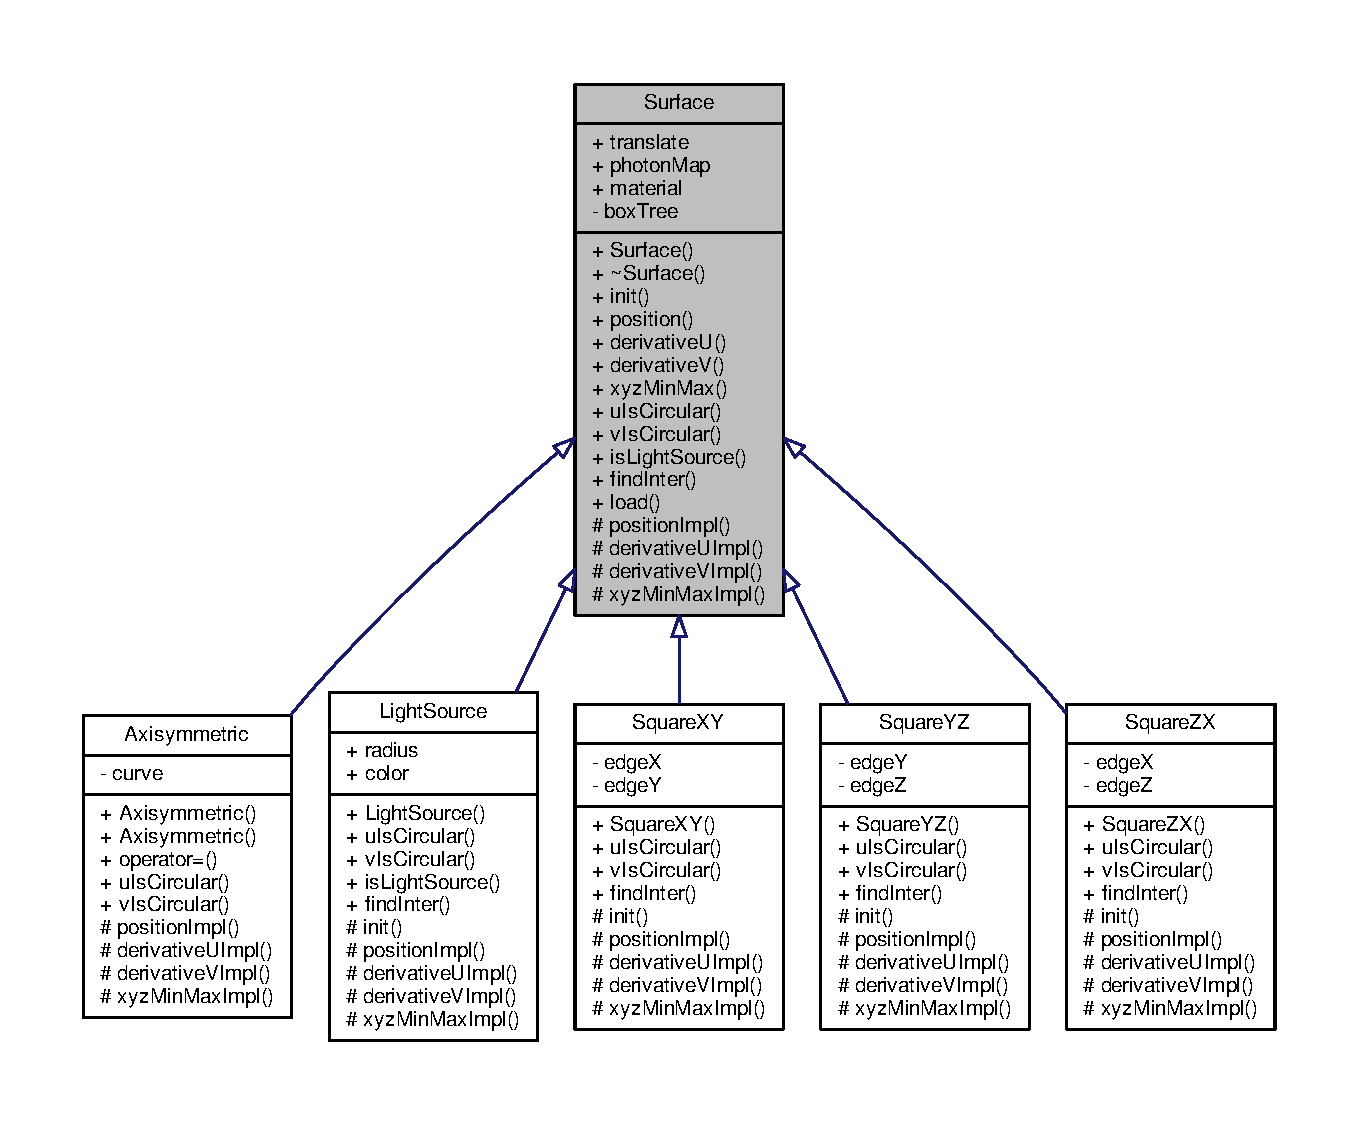
\includegraphics[width=350pt]{classSurface__inherit__graph}
\end{center}
\end{figure}


Collaboration diagram for Surface\+:\nopagebreak
\begin{figure}[H]
\begin{center}
\leavevmode
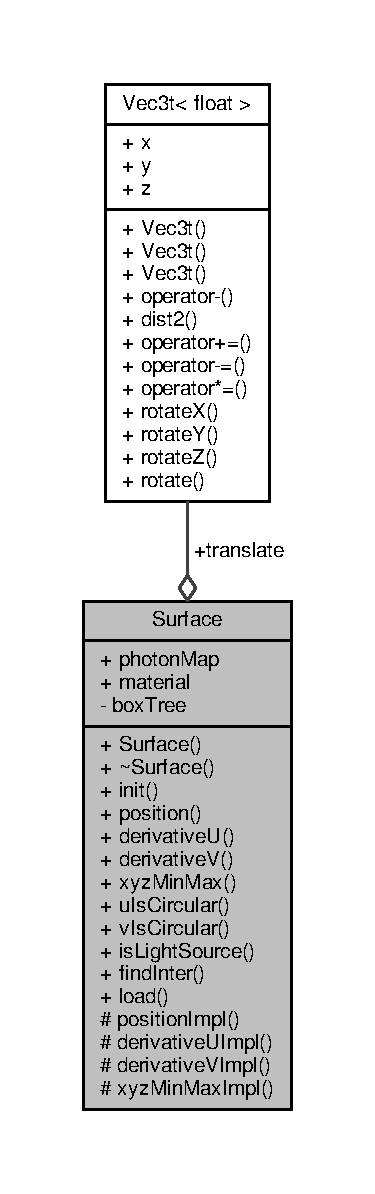
\includegraphics[height=550pt]{classSurface__coll__graph}
\end{center}
\end{figure}
\subsection*{Public Member Functions}
\begin{DoxyCompactItemize}
\item 
\hyperlink{classSurface_a8fc57f2a15292135c00545c9d224ec68}{Surface} ()
\item 
virtual \hyperlink{classSurface_a44ff6a911acc4ada428c3d734f342a8a}{$\sim$\+Surface} ()
\item 
virtual void \hyperlink{classSurface_a194087202684a4b3a71c24f02faeb404}{init} ()
\begin{DoxyCompactList}\small\item\em Something can\textquotesingle{}t be put in constructor. \end{DoxyCompactList}\item 
\hyperlink{vec_8h_ae4fcaa7c0a3935930ed1be5f70b90373}{Vec3} \hyperlink{classSurface_ac7eb5876716281ea19945829ff9114b3}{position} (float u, float v) const 
\begin{DoxyCompactList}\small\item\em Get point on the surface. \end{DoxyCompactList}\item 
\hyperlink{vec_8h_ae4fcaa7c0a3935930ed1be5f70b90373}{Vec3} \hyperlink{classSurface_a3b60891745ce4a2dc1adc379fc69b866}{derivativeU} (float u, float v) const 
\begin{DoxyCompactList}\small\item\em Get partial S / partial u on the surface. \end{DoxyCompactList}\item 
\hyperlink{vec_8h_ae4fcaa7c0a3935930ed1be5f70b90373}{Vec3} \hyperlink{classSurface_a0c8bd80201b1426d30781d9583e86afd}{derivativeV} (float u, float v) const 
\begin{DoxyCompactList}\small\item\em Get partial S / partial v on the surface. \end{DoxyCompactList}\item 
\hyperlink{structBox3}{Box3} \hyperlink{classSurface_aef6ac6d0bd8f7db26b85f140e4ed2ea8}{xyz\+Min\+Max} (float u1, float u2, float v1, float v2) const 
\begin{DoxyCompactList}\small\item\em (x\+:(min, max), y\+:(min, max), z\+: (min, max)) when (u,v) in \mbox{[}u1, u2\mbox{]} $\ast$ \mbox{[}v1, v2\mbox{]} \end{DoxyCompactList}\item 
virtual bool \hyperlink{classSurface_a11d5759ec3e3d43036fb949dcc6f5562}{u\+Is\+Circular} () const =0
\item 
virtual bool \hyperlink{classSurface_af52f9322929a702a9aaeee3ae4a368da}{v\+Is\+Circular} () const =0
\item 
virtual bool \hyperlink{classSurface_a5968cee515dd97f1e5066fec7cbf9b03}{is\+Light\+Source} () const 
\item 
virtual \hyperlink{classOptional}{Optional}$<$ \hyperlink{structSurfInterType}{Surf\+Inter\+Type} $>$ \hyperlink{classSurface_af7b5584007bf626bf7b37fcf649e6cd6}{find\+Inter} (const \hyperlink{structRay}{Ray} \&ray) const 
\begin{DoxyCompactList}\small\item\em Find intersection on 1 surface. \end{DoxyCompactList}\end{DoxyCompactItemize}
\subsection*{Static Public Member Functions}
\begin{DoxyCompactItemize}
\item 
static std\+::vector$<$ std\+::unique\+\_\+ptr$<$ \hyperlink{classSurface}{Surface} $>$ $>$ \hyperlink{classSurface_a73a61d351a694602ca76ac1ecb3937e9}{load} (const char filename\mbox{[}$\,$\mbox{]})
\begin{DoxyCompactList}\small\item\em Load surfaces from file. \end{DoxyCompactList}\end{DoxyCompactItemize}
\subsection*{Public Attributes}
\begin{DoxyCompactItemize}
\item 
\hyperlink{vec_8h_ae4fcaa7c0a3935930ed1be5f70b90373}{Vec3} \hyperlink{classSurface_a442734b024ed1013878d098d27ade6ad}{translate}
\item 
std\+::unique\+\_\+ptr$<$ \hyperlink{classPhotonMap}{Photon\+Map} $>$ \hyperlink{classSurface_aa624ee597db52c7c8f341e5a31b9e279}{photon\+Map}
\item 
std\+::unique\+\_\+ptr$<$ \hyperlink{structMaterial}{Material} $>$ \hyperlink{classSurface_aa68847b731186c38991568c5925ad862}{material}
\end{DoxyCompactItemize}
\subsection*{Protected Member Functions}
\begin{DoxyCompactItemize}
\item 
virtual \hyperlink{vec_8h_ae4fcaa7c0a3935930ed1be5f70b90373}{Vec3} \hyperlink{classSurface_a379545eea4809f81fe7e037f5e5ff4be}{position\+Impl} (float u, float v) const =0
\item 
virtual \hyperlink{vec_8h_ae4fcaa7c0a3935930ed1be5f70b90373}{Vec3} \hyperlink{classSurface_a4de8fb9d4652cc32022c95eb903cce4a}{derivative\+U\+Impl} (float u, float v) const =0
\item 
virtual \hyperlink{vec_8h_ae4fcaa7c0a3935930ed1be5f70b90373}{Vec3} \hyperlink{classSurface_a95d65437419ba8d439fa8f0d71f963a1}{derivative\+V\+Impl} (float u, float v) const =0
\item 
virtual \hyperlink{structBox3}{Box3} \hyperlink{classSurface_ab1ee990da290748cd86aaf95edb28c38}{xyz\+Min\+Max\+Impl} (float u1, float u2, float v1, float v2) const =0
\end{DoxyCompactItemize}
\subsection*{Private Attributes}
\begin{DoxyCompactItemize}
\item 
std\+::unique\+\_\+ptr$<$ \hyperlink{classBoxTree}{Box\+Tree} $>$ \hyperlink{classSurface_a0620b2906ff595d71dedec53ff75b924}{box\+Tree}
\end{DoxyCompactItemize}


\subsection{Detailed Description}
\hyperlink{classSurface}{Surface} base class \hyperlink{classSurface}{Surface} decided by parameter (u,v) in \mbox{[}0,1\mbox{]} $\ast$ \mbox{[}0,1\mbox{]}. 

\subsection{Constructor \& Destructor Documentation}
\index{Surface@{Surface}!Surface@{Surface}}
\index{Surface@{Surface}!Surface@{Surface}}
\subsubsection[{\texorpdfstring{Surface()}{Surface()}}]{\setlength{\rightskip}{0pt plus 5cm}Surface\+::\+Surface (
\begin{DoxyParamCaption}
{}
\end{DoxyParamCaption}
)\hspace{0.3cm}{\ttfamily [inline]}}\hypertarget{classSurface_a8fc57f2a15292135c00545c9d224ec68}{}\label{classSurface_a8fc57f2a15292135c00545c9d224ec68}
\index{Surface@{Surface}!````~Surface@{$\sim$\+Surface}}
\index{````~Surface@{$\sim$\+Surface}!Surface@{Surface}}
\subsubsection[{\texorpdfstring{$\sim$\+Surface()}{~Surface()}}]{\setlength{\rightskip}{0pt plus 5cm}virtual Surface\+::$\sim$\+Surface (
\begin{DoxyParamCaption}
{}
\end{DoxyParamCaption}
)\hspace{0.3cm}{\ttfamily [inline]}, {\ttfamily [virtual]}}\hypertarget{classSurface_a44ff6a911acc4ada428c3d734f342a8a}{}\label{classSurface_a44ff6a911acc4ada428c3d734f342a8a}


\subsection{Member Function Documentation}
\index{Surface@{Surface}!derivativeU@{derivativeU}}
\index{derivativeU@{derivativeU}!Surface@{Surface}}
\subsubsection[{\texorpdfstring{derivative\+U(float u, float v) const }{derivativeU(float u, float v) const }}]{\setlength{\rightskip}{0pt plus 5cm}{\bf Vec3} Surface\+::derivativeU (
\begin{DoxyParamCaption}
\item[{float}]{u, }
\item[{float}]{v}
\end{DoxyParamCaption}
) const\hspace{0.3cm}{\ttfamily [inline]}}\hypertarget{classSurface_a3b60891745ce4a2dc1adc379fc69b866}{}\label{classSurface_a3b60891745ce4a2dc1adc379fc69b866}


Get partial S / partial u on the surface. 

\index{Surface@{Surface}!derivative\+U\+Impl@{derivative\+U\+Impl}}
\index{derivative\+U\+Impl@{derivative\+U\+Impl}!Surface@{Surface}}
\subsubsection[{\texorpdfstring{derivative\+U\+Impl(float u, float v) const =0}{derivativeUImpl(float u, float v) const =0}}]{\setlength{\rightskip}{0pt plus 5cm}virtual {\bf Vec3} Surface\+::derivative\+U\+Impl (
\begin{DoxyParamCaption}
\item[{float}]{u, }
\item[{float}]{v}
\end{DoxyParamCaption}
) const\hspace{0.3cm}{\ttfamily [protected]}, {\ttfamily [pure virtual]}}\hypertarget{classSurface_a4de8fb9d4652cc32022c95eb903cce4a}{}\label{classSurface_a4de8fb9d4652cc32022c95eb903cce4a}


Implemented in \hyperlink{classLightSource_ac9506b1c3f773b0de0c30ca78b4a9aa0}{Light\+Source}, \hyperlink{classAxisymmetric_a2af551bce6cffc034a278de5c2f5f3c4}{Axisymmetric}, \hyperlink{classSquareXY_a7507f187a31f589c06afe6dbcbccfe46}{Square\+XY}, \hyperlink{classSquareYZ_a2b37c54c61d5f2896657f8510884e64e}{Square\+YZ}, and \hyperlink{classSquareZX_aafd9b0bfc12a6034d07d4cf27b211cfd}{Square\+ZX}.

\index{Surface@{Surface}!derivativeV@{derivativeV}}
\index{derivativeV@{derivativeV}!Surface@{Surface}}
\subsubsection[{\texorpdfstring{derivative\+V(float u, float v) const }{derivativeV(float u, float v) const }}]{\setlength{\rightskip}{0pt plus 5cm}{\bf Vec3} Surface\+::derivativeV (
\begin{DoxyParamCaption}
\item[{float}]{u, }
\item[{float}]{v}
\end{DoxyParamCaption}
) const\hspace{0.3cm}{\ttfamily [inline]}}\hypertarget{classSurface_a0c8bd80201b1426d30781d9583e86afd}{}\label{classSurface_a0c8bd80201b1426d30781d9583e86afd}


Get partial S / partial v on the surface. 

\index{Surface@{Surface}!derivative\+V\+Impl@{derivative\+V\+Impl}}
\index{derivative\+V\+Impl@{derivative\+V\+Impl}!Surface@{Surface}}
\subsubsection[{\texorpdfstring{derivative\+V\+Impl(float u, float v) const =0}{derivativeVImpl(float u, float v) const =0}}]{\setlength{\rightskip}{0pt plus 5cm}virtual {\bf Vec3} Surface\+::derivative\+V\+Impl (
\begin{DoxyParamCaption}
\item[{float}]{u, }
\item[{float}]{v}
\end{DoxyParamCaption}
) const\hspace{0.3cm}{\ttfamily [protected]}, {\ttfamily [pure virtual]}}\hypertarget{classSurface_a95d65437419ba8d439fa8f0d71f963a1}{}\label{classSurface_a95d65437419ba8d439fa8f0d71f963a1}


Implemented in \hyperlink{classLightSource_a90b1596aca4c3b818fe73d8ef35065da}{Light\+Source}, \hyperlink{classAxisymmetric_ab62630c58ba420d44eb39753f27abba9}{Axisymmetric}, \hyperlink{classSquareXY_a4803259cb98c12ba97eb9e8c57463b2d}{Square\+XY}, \hyperlink{classSquareYZ_a6fc7a2189bf889b0dd99c229d2a6d0da}{Square\+YZ}, and \hyperlink{classSquareZX_a3ede3591078b049a8997ad144d7f92cd}{Square\+ZX}.

\index{Surface@{Surface}!find\+Inter@{find\+Inter}}
\index{find\+Inter@{find\+Inter}!Surface@{Surface}}
\subsubsection[{\texorpdfstring{find\+Inter(const Ray \&ray) const }{findInter(const Ray &ray) const }}]{\setlength{\rightskip}{0pt plus 5cm}{\bf Optional}$<$ {\bf Surf\+Inter\+Type} $>$ Surface\+::find\+Inter (
\begin{DoxyParamCaption}
\item[{const {\bf Ray} \&}]{ray}
\end{DoxyParamCaption}
) const\hspace{0.3cm}{\ttfamily [virtual]}}\hypertarget{classSurface_af7b5584007bf626bf7b37fcf649e6cd6}{}\label{classSurface_af7b5584007bf626bf7b37fcf649e6cd6}


Find intersection on 1 surface. 



Reimplemented in \hyperlink{classLightSource_a7470bd637b7013e310c1a6789d12de92}{Light\+Source}, \hyperlink{classSquareXY_a33545d952933da0107ca9d9a6c8301ff}{Square\+XY}, \hyperlink{classSquareYZ_a75ffd1eda4c026706513dfa07043ffc8}{Square\+YZ}, and \hyperlink{classSquareZX_a2de50bbf52fc3243eaf1b68099224321}{Square\+ZX}.

\index{Surface@{Surface}!init@{init}}
\index{init@{init}!Surface@{Surface}}
\subsubsection[{\texorpdfstring{init()}{init()}}]{\setlength{\rightskip}{0pt plus 5cm}void Surface\+::init (
\begin{DoxyParamCaption}
{}
\end{DoxyParamCaption}
)\hspace{0.3cm}{\ttfamily [virtual]}}\hypertarget{classSurface_a194087202684a4b3a71c24f02faeb404}{}\label{classSurface_a194087202684a4b3a71c24f02faeb404}


Something can\textquotesingle{}t be put in constructor. 



Reimplemented in \hyperlink{classLightSource_a9001c11824ce30f44bdd9a729cc420a6}{Light\+Source}, \hyperlink{classSquareXY_a9dfeebdb190f64c6085625e2dcf7d400}{Square\+XY}, \hyperlink{classSquareYZ_a1d82d4fea479dd58096d723eb9109cfe}{Square\+YZ}, and \hyperlink{classSquareZX_aefbaa1f1b673aa405f427dbacc81114c}{Square\+ZX}.

\index{Surface@{Surface}!is\+Light\+Source@{is\+Light\+Source}}
\index{is\+Light\+Source@{is\+Light\+Source}!Surface@{Surface}}
\subsubsection[{\texorpdfstring{is\+Light\+Source() const }{isLightSource() const }}]{\setlength{\rightskip}{0pt plus 5cm}virtual bool Surface\+::is\+Light\+Source (
\begin{DoxyParamCaption}
{}
\end{DoxyParamCaption}
) const\hspace{0.3cm}{\ttfamily [inline]}, {\ttfamily [virtual]}}\hypertarget{classSurface_a5968cee515dd97f1e5066fec7cbf9b03}{}\label{classSurface_a5968cee515dd97f1e5066fec7cbf9b03}


Reimplemented in \hyperlink{classLightSource_a5d397dd1719c8aaf9d711bace27a9547}{Light\+Source}.

\index{Surface@{Surface}!load@{load}}
\index{load@{load}!Surface@{Surface}}
\subsubsection[{\texorpdfstring{load(const char filename[])}{load(const char filename[])}}]{\setlength{\rightskip}{0pt plus 5cm}std\+::vector$<$ std\+::unique\+\_\+ptr$<$ {\bf Surface} $>$ $>$ Surface\+::load (
\begin{DoxyParamCaption}
\item[{const char}]{filename\mbox{[}$\,$\mbox{]}}
\end{DoxyParamCaption}
)\hspace{0.3cm}{\ttfamily [static]}}\hypertarget{classSurface_a73a61d351a694602ca76ac1ecb3937e9}{}\label{classSurface_a73a61d351a694602ca76ac1ecb3937e9}


Load surfaces from file. 

\index{Surface@{Surface}!position@{position}}
\index{position@{position}!Surface@{Surface}}
\subsubsection[{\texorpdfstring{position(float u, float v) const }{position(float u, float v) const }}]{\setlength{\rightskip}{0pt plus 5cm}{\bf Vec3} Surface\+::position (
\begin{DoxyParamCaption}
\item[{float}]{u, }
\item[{float}]{v}
\end{DoxyParamCaption}
) const\hspace{0.3cm}{\ttfamily [inline]}}\hypertarget{classSurface_ac7eb5876716281ea19945829ff9114b3}{}\label{classSurface_ac7eb5876716281ea19945829ff9114b3}


Get point on the surface. 

\index{Surface@{Surface}!position\+Impl@{position\+Impl}}
\index{position\+Impl@{position\+Impl}!Surface@{Surface}}
\subsubsection[{\texorpdfstring{position\+Impl(float u, float v) const =0}{positionImpl(float u, float v) const =0}}]{\setlength{\rightskip}{0pt plus 5cm}virtual {\bf Vec3} Surface\+::position\+Impl (
\begin{DoxyParamCaption}
\item[{float}]{u, }
\item[{float}]{v}
\end{DoxyParamCaption}
) const\hspace{0.3cm}{\ttfamily [protected]}, {\ttfamily [pure virtual]}}\hypertarget{classSurface_a379545eea4809f81fe7e037f5e5ff4be}{}\label{classSurface_a379545eea4809f81fe7e037f5e5ff4be}


Implemented in \hyperlink{classLightSource_a1ac118f57425ed163c6ab45d6320f401}{Light\+Source}, \hyperlink{classAxisymmetric_a65f503a73188b0647945bf3a6a5b901e}{Axisymmetric}, \hyperlink{classSquareXY_a3d47992c4b73c6f49bade1c7e3fe05fe}{Square\+XY}, \hyperlink{classSquareYZ_a56695f7f1cbd288bf93918deac0feb4c}{Square\+YZ}, and \hyperlink{classSquareZX_a505da0c732d570991b69837e9dac89e5}{Square\+ZX}.

\index{Surface@{Surface}!u\+Is\+Circular@{u\+Is\+Circular}}
\index{u\+Is\+Circular@{u\+Is\+Circular}!Surface@{Surface}}
\subsubsection[{\texorpdfstring{u\+Is\+Circular() const =0}{uIsCircular() const =0}}]{\setlength{\rightskip}{0pt plus 5cm}virtual bool Surface\+::u\+Is\+Circular (
\begin{DoxyParamCaption}
{}
\end{DoxyParamCaption}
) const\hspace{0.3cm}{\ttfamily [pure virtual]}}\hypertarget{classSurface_a11d5759ec3e3d43036fb949dcc6f5562}{}\label{classSurface_a11d5759ec3e3d43036fb949dcc6f5562}


Implemented in \hyperlink{classAxisymmetric_a50b489a9914ad852638b586cc0c6c2dc}{Axisymmetric}, \hyperlink{classLightSource_a6d1e29c394c2ae29c6b913376a3ebbc5}{Light\+Source}, \hyperlink{classSquareXY_a060cba6cee229bbe185bd59fbc49c461}{Square\+XY}, \hyperlink{classSquareYZ_adc74593250e7aaf7f8d733e22e3951b6}{Square\+YZ}, and \hyperlink{classSquareZX_a912de0928a8332afb6cb89179595668a}{Square\+ZX}.

\index{Surface@{Surface}!v\+Is\+Circular@{v\+Is\+Circular}}
\index{v\+Is\+Circular@{v\+Is\+Circular}!Surface@{Surface}}
\subsubsection[{\texorpdfstring{v\+Is\+Circular() const =0}{vIsCircular() const =0}}]{\setlength{\rightskip}{0pt plus 5cm}virtual bool Surface\+::v\+Is\+Circular (
\begin{DoxyParamCaption}
{}
\end{DoxyParamCaption}
) const\hspace{0.3cm}{\ttfamily [pure virtual]}}\hypertarget{classSurface_af52f9322929a702a9aaeee3ae4a368da}{}\label{classSurface_af52f9322929a702a9aaeee3ae4a368da}


Implemented in \hyperlink{classAxisymmetric_a63d63250b3ca2a34c2707abf35169657}{Axisymmetric}, \hyperlink{classLightSource_a617519569f55a575189f0de58f0b8a11}{Light\+Source}, \hyperlink{classSquareXY_aeebe33da47d345225afba03b8aa110dc}{Square\+XY}, \hyperlink{classSquareYZ_ab6a94e65acedccedd4556023b1490841}{Square\+YZ}, and \hyperlink{classSquareZX_a5556f34a0c9e6c07f59c488857937b35}{Square\+ZX}.

\index{Surface@{Surface}!xyz\+Min\+Max@{xyz\+Min\+Max}}
\index{xyz\+Min\+Max@{xyz\+Min\+Max}!Surface@{Surface}}
\subsubsection[{\texorpdfstring{xyz\+Min\+Max(float u1, float u2, float v1, float v2) const }{xyzMinMax(float u1, float u2, float v1, float v2) const }}]{\setlength{\rightskip}{0pt plus 5cm}{\bf Box3} Surface\+::xyz\+Min\+Max (
\begin{DoxyParamCaption}
\item[{float}]{u1, }
\item[{float}]{u2, }
\item[{float}]{v1, }
\item[{float}]{v2}
\end{DoxyParamCaption}
) const\hspace{0.3cm}{\ttfamily [inline]}}\hypertarget{classSurface_aef6ac6d0bd8f7db26b85f140e4ed2ea8}{}\label{classSurface_aef6ac6d0bd8f7db26b85f140e4ed2ea8}


(x\+:(min, max), y\+:(min, max), z\+: (min, max)) when (u,v) in \mbox{[}u1, u2\mbox{]} $\ast$ \mbox{[}v1, v2\mbox{]} 

\index{Surface@{Surface}!xyz\+Min\+Max\+Impl@{xyz\+Min\+Max\+Impl}}
\index{xyz\+Min\+Max\+Impl@{xyz\+Min\+Max\+Impl}!Surface@{Surface}}
\subsubsection[{\texorpdfstring{xyz\+Min\+Max\+Impl(float u1, float u2, float v1, float v2) const =0}{xyzMinMaxImpl(float u1, float u2, float v1, float v2) const =0}}]{\setlength{\rightskip}{0pt plus 5cm}virtual {\bf Box3} Surface\+::xyz\+Min\+Max\+Impl (
\begin{DoxyParamCaption}
\item[{float}]{u1, }
\item[{float}]{u2, }
\item[{float}]{v1, }
\item[{float}]{v2}
\end{DoxyParamCaption}
) const\hspace{0.3cm}{\ttfamily [protected]}, {\ttfamily [pure virtual]}}\hypertarget{classSurface_ab1ee990da290748cd86aaf95edb28c38}{}\label{classSurface_ab1ee990da290748cd86aaf95edb28c38}


Implemented in \hyperlink{classLightSource_a01f7d7c1cca3b8ab7ec688253a46aaec}{Light\+Source}, \hyperlink{classAxisymmetric_a2718336bc4e05234a3f57bbe80ec29d3}{Axisymmetric}, \hyperlink{classSquareXY_ae03eb06fd6a8b493ebd1acbb0d22f365}{Square\+XY}, \hyperlink{classSquareYZ_a61260b3bae72f9354a8fe4c145bce87d}{Square\+YZ}, and \hyperlink{classSquareZX_a87b224b775e24f1d6ba984d37d0c85eb}{Square\+ZX}.



\subsection{Member Data Documentation}
\index{Surface@{Surface}!box\+Tree@{box\+Tree}}
\index{box\+Tree@{box\+Tree}!Surface@{Surface}}
\subsubsection[{\texorpdfstring{box\+Tree}{boxTree}}]{\setlength{\rightskip}{0pt plus 5cm}std\+::unique\+\_\+ptr$<${\bf Box\+Tree}$>$ Surface\+::box\+Tree\hspace{0.3cm}{\ttfamily [private]}}\hypertarget{classSurface_a0620b2906ff595d71dedec53ff75b924}{}\label{classSurface_a0620b2906ff595d71dedec53ff75b924}
\index{Surface@{Surface}!material@{material}}
\index{material@{material}!Surface@{Surface}}
\subsubsection[{\texorpdfstring{material}{material}}]{\setlength{\rightskip}{0pt plus 5cm}std\+::unique\+\_\+ptr$<${\bf Material}$>$ Surface\+::material}\hypertarget{classSurface_aa68847b731186c38991568c5925ad862}{}\label{classSurface_aa68847b731186c38991568c5925ad862}
\index{Surface@{Surface}!photon\+Map@{photon\+Map}}
\index{photon\+Map@{photon\+Map}!Surface@{Surface}}
\subsubsection[{\texorpdfstring{photon\+Map}{photonMap}}]{\setlength{\rightskip}{0pt plus 5cm}std\+::unique\+\_\+ptr$<${\bf Photon\+Map}$>$ Surface\+::photon\+Map}\hypertarget{classSurface_aa624ee597db52c7c8f341e5a31b9e279}{}\label{classSurface_aa624ee597db52c7c8f341e5a31b9e279}
\index{Surface@{Surface}!translate@{translate}}
\index{translate@{translate}!Surface@{Surface}}
\subsubsection[{\texorpdfstring{translate}{translate}}]{\setlength{\rightskip}{0pt plus 5cm}{\bf Vec3} Surface\+::translate}\hypertarget{classSurface_a442734b024ed1013878d098d27ade6ad}{}\label{classSurface_a442734b024ed1013878d098d27ade6ad}


The documentation for this class was generated from the following files\+:\begin{DoxyCompactItemize}
\item 
\hyperlink{surface_8h}{surface.\+h}\item 
\hyperlink{surface_8cpp}{surface.\+cpp}\end{DoxyCompactItemize}

\hypertarget{structSurfInterType}{}\section{Surf\+Inter\+Type Struct Reference}
\label{structSurfInterType}\index{Surf\+Inter\+Type@{Surf\+Inter\+Type}}


{\ttfamily \#include $<$intersection.\+h$>$}



Collaboration diagram for Surf\+Inter\+Type\+:
\nopagebreak
\begin{figure}[H]
\begin{center}
\leavevmode
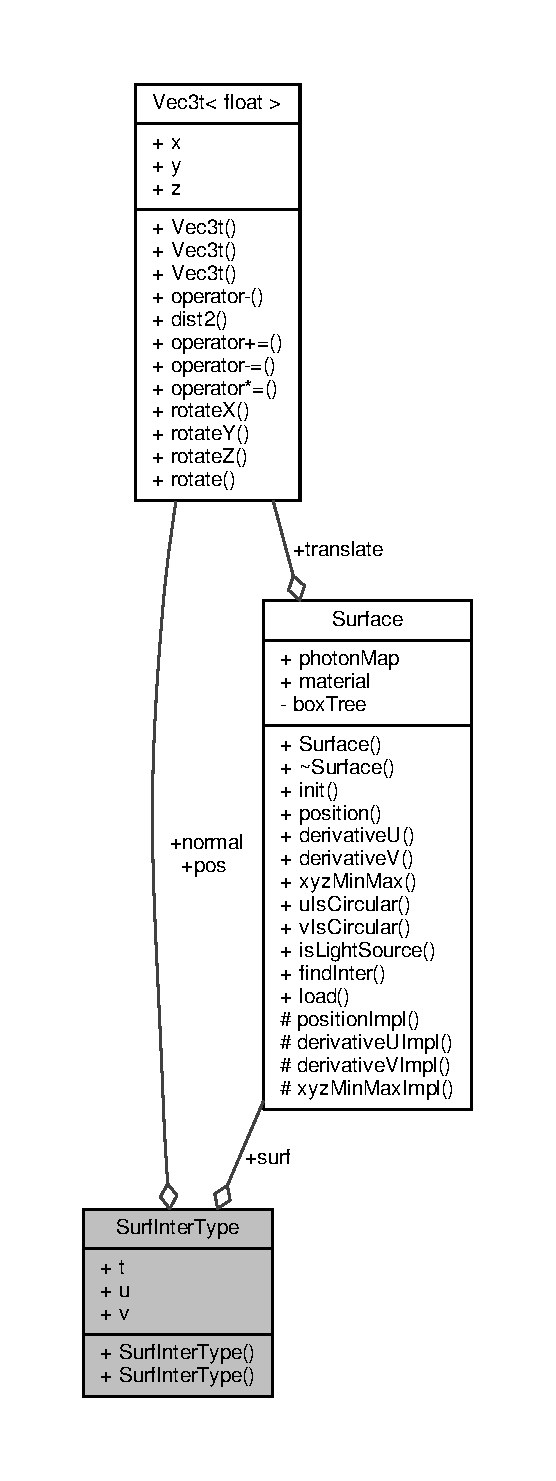
\includegraphics[height=550pt]{structSurfInterType__coll__graph}
\end{center}
\end{figure}
\subsection*{Public Member Functions}
\begin{DoxyCompactItemize}
\item 
\hyperlink{structSurfInterType_a009e048cba0eb369863e36d87f976937}{Surf\+Inter\+Type} ()
\item 
\hyperlink{structSurfInterType_afbbdcc212c382a20b7722285b21407a3}{Surf\+Inter\+Type} (const \hyperlink{classSurface}{Surface} $\ast$\+\_\+surf, float \+\_\+t, float \+\_\+u, float \+\_\+v, const \hyperlink{vec_8h_ae4fcaa7c0a3935930ed1be5f70b90373}{Vec3} \&\+\_\+pos, const \hyperlink{vec_8h_ae4fcaa7c0a3935930ed1be5f70b90373}{Vec3} \&\+\_\+normal)
\end{DoxyCompactItemize}
\subsection*{Public Attributes}
\begin{DoxyCompactItemize}
\item 
const \hyperlink{classSurface}{Surface} $\ast$ \hyperlink{structSurfInterType_a257b9ee9e47864c03a15495d646737e1}{surf}
\item 
float \hyperlink{structSurfInterType_a858293669930005f19a35357f2514752}{t}
\item 
float \hyperlink{structSurfInterType_a55d18e6bdaf4d40084f772610ff8c3d2}{u}
\item 
float \hyperlink{structSurfInterType_a49f68075edc5d8aa37aef1239ae5ca40}{v}
\item 
\hyperlink{vec_8h_ae4fcaa7c0a3935930ed1be5f70b90373}{Vec3} \hyperlink{structSurfInterType_aca92cd7c249fe62ecde0fbc6076abe8b}{pos}
\item 
\hyperlink{vec_8h_ae4fcaa7c0a3935930ed1be5f70b90373}{Vec3} \hyperlink{structSurfInterType_ad990ea8d9f0347bb405e7d6bb33d45ae}{normal}
\end{DoxyCompactItemize}


\subsection{Constructor \& Destructor Documentation}
\index{Surf\+Inter\+Type@{Surf\+Inter\+Type}!Surf\+Inter\+Type@{Surf\+Inter\+Type}}
\index{Surf\+Inter\+Type@{Surf\+Inter\+Type}!Surf\+Inter\+Type@{Surf\+Inter\+Type}}
\subsubsection[{\texorpdfstring{Surf\+Inter\+Type()}{SurfInterType()}}]{\setlength{\rightskip}{0pt plus 5cm}Surf\+Inter\+Type\+::\+Surf\+Inter\+Type (
\begin{DoxyParamCaption}
{}
\end{DoxyParamCaption}
)\hspace{0.3cm}{\ttfamily [inline]}}\hypertarget{structSurfInterType_a009e048cba0eb369863e36d87f976937}{}\label{structSurfInterType_a009e048cba0eb369863e36d87f976937}
\index{Surf\+Inter\+Type@{Surf\+Inter\+Type}!Surf\+Inter\+Type@{Surf\+Inter\+Type}}
\index{Surf\+Inter\+Type@{Surf\+Inter\+Type}!Surf\+Inter\+Type@{Surf\+Inter\+Type}}
\subsubsection[{\texorpdfstring{Surf\+Inter\+Type(const Surface $\ast$\+\_\+surf, float \+\_\+t, float \+\_\+u, float \+\_\+v, const Vec3 \&\+\_\+pos, const Vec3 \&\+\_\+normal)}{SurfInterType(const Surface *_surf, float _t, float _u, float _v, const Vec3 &_pos, const Vec3 &_normal)}}]{\setlength{\rightskip}{0pt plus 5cm}Surf\+Inter\+Type\+::\+Surf\+Inter\+Type (
\begin{DoxyParamCaption}
\item[{const {\bf Surface} $\ast$}]{\+\_\+surf, }
\item[{float}]{\+\_\+t, }
\item[{float}]{\+\_\+u, }
\item[{float}]{\+\_\+v, }
\item[{const {\bf Vec3} \&}]{\+\_\+pos, }
\item[{const {\bf Vec3} \&}]{\+\_\+normal}
\end{DoxyParamCaption}
)\hspace{0.3cm}{\ttfamily [inline]}}\hypertarget{structSurfInterType_afbbdcc212c382a20b7722285b21407a3}{}\label{structSurfInterType_afbbdcc212c382a20b7722285b21407a3}


\subsection{Member Data Documentation}
\index{Surf\+Inter\+Type@{Surf\+Inter\+Type}!normal@{normal}}
\index{normal@{normal}!Surf\+Inter\+Type@{Surf\+Inter\+Type}}
\subsubsection[{\texorpdfstring{normal}{normal}}]{\setlength{\rightskip}{0pt plus 5cm}{\bf Vec3} Surf\+Inter\+Type\+::normal}\hypertarget{structSurfInterType_ad990ea8d9f0347bb405e7d6bb33d45ae}{}\label{structSurfInterType_ad990ea8d9f0347bb405e7d6bb33d45ae}
\index{Surf\+Inter\+Type@{Surf\+Inter\+Type}!pos@{pos}}
\index{pos@{pos}!Surf\+Inter\+Type@{Surf\+Inter\+Type}}
\subsubsection[{\texorpdfstring{pos}{pos}}]{\setlength{\rightskip}{0pt plus 5cm}{\bf Vec3} Surf\+Inter\+Type\+::pos}\hypertarget{structSurfInterType_aca92cd7c249fe62ecde0fbc6076abe8b}{}\label{structSurfInterType_aca92cd7c249fe62ecde0fbc6076abe8b}
\index{Surf\+Inter\+Type@{Surf\+Inter\+Type}!surf@{surf}}
\index{surf@{surf}!Surf\+Inter\+Type@{Surf\+Inter\+Type}}
\subsubsection[{\texorpdfstring{surf}{surf}}]{\setlength{\rightskip}{0pt plus 5cm}const {\bf Surface}$\ast$ Surf\+Inter\+Type\+::surf}\hypertarget{structSurfInterType_a257b9ee9e47864c03a15495d646737e1}{}\label{structSurfInterType_a257b9ee9e47864c03a15495d646737e1}
\index{Surf\+Inter\+Type@{Surf\+Inter\+Type}!t@{t}}
\index{t@{t}!Surf\+Inter\+Type@{Surf\+Inter\+Type}}
\subsubsection[{\texorpdfstring{t}{t}}]{\setlength{\rightskip}{0pt plus 5cm}float Surf\+Inter\+Type\+::t}\hypertarget{structSurfInterType_a858293669930005f19a35357f2514752}{}\label{structSurfInterType_a858293669930005f19a35357f2514752}
\index{Surf\+Inter\+Type@{Surf\+Inter\+Type}!u@{u}}
\index{u@{u}!Surf\+Inter\+Type@{Surf\+Inter\+Type}}
\subsubsection[{\texorpdfstring{u}{u}}]{\setlength{\rightskip}{0pt plus 5cm}float Surf\+Inter\+Type\+::u}\hypertarget{structSurfInterType_a55d18e6bdaf4d40084f772610ff8c3d2}{}\label{structSurfInterType_a55d18e6bdaf4d40084f772610ff8c3d2}
\index{Surf\+Inter\+Type@{Surf\+Inter\+Type}!v@{v}}
\index{v@{v}!Surf\+Inter\+Type@{Surf\+Inter\+Type}}
\subsubsection[{\texorpdfstring{v}{v}}]{\setlength{\rightskip}{0pt plus 5cm}float Surf\+Inter\+Type\+::v}\hypertarget{structSurfInterType_a49f68075edc5d8aa37aef1239ae5ca40}{}\label{structSurfInterType_a49f68075edc5d8aa37aef1239ae5ca40}


The documentation for this struct was generated from the following file\+:\begin{DoxyCompactItemize}
\item 
\hyperlink{intersection_8h}{intersection.\+h}\end{DoxyCompactItemize}

\hypertarget{classTexture}{}\section{Texture Class Reference}
\label{classTexture}\index{Texture@{Texture}}


{\ttfamily \#include $<$texture.\+h$>$}



Collaboration diagram for Texture\+:
\nopagebreak
\begin{figure}[H]
\begin{center}
\leavevmode
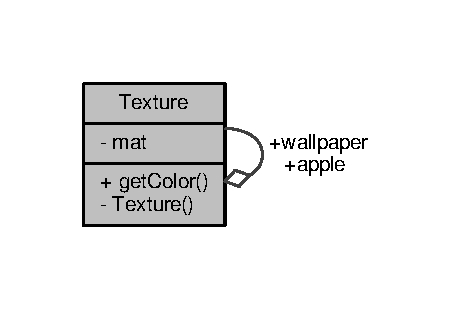
\includegraphics[width=217pt]{classTexture__coll__graph}
\end{center}
\end{figure}
\subsection*{Public Member Functions}
\begin{DoxyCompactItemize}
\item 
\hyperlink{ray_8h_a8a2580fb65f7d3d4e24bdd412b9bd92d}{color\+\_\+t} \hyperlink{classTexture_a78e72a36da8f70603b2753b302c97330}{get\+Color} (float u, float v)
\end{DoxyCompactItemize}
\subsection*{Static Public Attributes}
\begin{DoxyCompactItemize}
\item 
static \hyperlink{classTexture}{Texture} \hyperlink{classTexture_a1fe6c8c86fe00b7f58d874c136b632ba}{wallpaper}
\item 
static \hyperlink{classTexture}{Texture} \hyperlink{classTexture_ae94748846788a55df372cc9152f829dd}{apple}
\end{DoxyCompactItemize}
\subsection*{Private Member Functions}
\begin{DoxyCompactItemize}
\item 
\hyperlink{classTexture_a8ad76d451ccb9732598137702887136b}{Texture} (const char filename\mbox{[}$\,$\mbox{]})
\end{DoxyCompactItemize}
\subsection*{Private Attributes}
\begin{DoxyCompactItemize}
\item 
cv\+::\+Mat3b \hyperlink{classTexture_a5d776b17260e556ee5bd94cbbd412413}{mat}
\end{DoxyCompactItemize}


\subsection{Constructor \& Destructor Documentation}
\index{Texture@{Texture}!Texture@{Texture}}
\index{Texture@{Texture}!Texture@{Texture}}
\subsubsection[{\texorpdfstring{Texture(const char filename[])}{Texture(const char filename[])}}]{\setlength{\rightskip}{0pt plus 5cm}Texture\+::\+Texture (
\begin{DoxyParamCaption}
\item[{const char}]{filename\mbox{[}$\,$\mbox{]}}
\end{DoxyParamCaption}
)\hspace{0.3cm}{\ttfamily [inline]}, {\ttfamily [private]}}\hypertarget{classTexture_a8ad76d451ccb9732598137702887136b}{}\label{classTexture_a8ad76d451ccb9732598137702887136b}


\subsection{Member Function Documentation}
\index{Texture@{Texture}!get\+Color@{get\+Color}}
\index{get\+Color@{get\+Color}!Texture@{Texture}}
\subsubsection[{\texorpdfstring{get\+Color(float u, float v)}{getColor(float u, float v)}}]{\setlength{\rightskip}{0pt plus 5cm}{\bf color\+\_\+t} Texture\+::get\+Color (
\begin{DoxyParamCaption}
\item[{float}]{u, }
\item[{float}]{v}
\end{DoxyParamCaption}
)\hspace{0.3cm}{\ttfamily [inline]}}\hypertarget{classTexture_a78e72a36da8f70603b2753b302c97330}{}\label{classTexture_a78e72a36da8f70603b2753b302c97330}


\subsection{Member Data Documentation}
\index{Texture@{Texture}!apple@{apple}}
\index{apple@{apple}!Texture@{Texture}}
\subsubsection[{\texorpdfstring{apple}{apple}}]{\setlength{\rightskip}{0pt plus 5cm}{\bf Texture} Texture\+::apple\hspace{0.3cm}{\ttfamily [static]}}\hypertarget{classTexture_ae94748846788a55df372cc9152f829dd}{}\label{classTexture_ae94748846788a55df372cc9152f829dd}
\index{Texture@{Texture}!mat@{mat}}
\index{mat@{mat}!Texture@{Texture}}
\subsubsection[{\texorpdfstring{mat}{mat}}]{\setlength{\rightskip}{0pt plus 5cm}cv\+::\+Mat3b Texture\+::mat\hspace{0.3cm}{\ttfamily [private]}}\hypertarget{classTexture_a5d776b17260e556ee5bd94cbbd412413}{}\label{classTexture_a5d776b17260e556ee5bd94cbbd412413}
\index{Texture@{Texture}!wallpaper@{wallpaper}}
\index{wallpaper@{wallpaper}!Texture@{Texture}}
\subsubsection[{\texorpdfstring{wallpaper}{wallpaper}}]{\setlength{\rightskip}{0pt plus 5cm}{\bf Texture} Texture\+::wallpaper\hspace{0.3cm}{\ttfamily [static]}}\hypertarget{classTexture_a1fe6c8c86fe00b7f58d874c136b632ba}{}\label{classTexture_a1fe6c8c86fe00b7f58d874c136b632ba}


The documentation for this class was generated from the following files\+:\begin{DoxyCompactItemize}
\item 
\hyperlink{texture_8h}{texture.\+h}\item 
\hyperlink{texture_8cpp}{texture.\+cpp}\end{DoxyCompactItemize}

\hypertarget{classTrace}{}\section{Trace Class Reference}
\label{classTrace}\index{Trace@{Trace}}


Perform tracing This is a static class.  




{\ttfamily \#include $<$trace.\+h$>$}



Collaboration diagram for Trace\+:\nopagebreak
\begin{figure}[H]
\begin{center}
\leavevmode
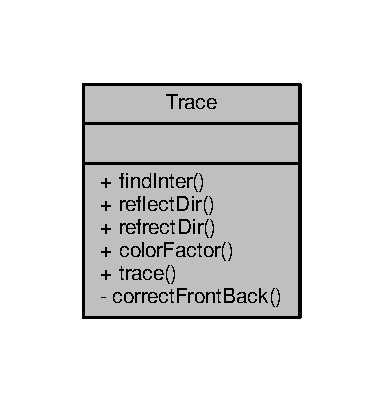
\includegraphics[width=184pt]{classTrace__coll__graph}
\end{center}
\end{figure}
\subsection*{Static Public Member Functions}
\begin{DoxyCompactItemize}
\item 
static \hyperlink{classOptional}{Optional}$<$ \hyperlink{structSurfInterType}{Surf\+Inter\+Type} $>$ \hyperlink{classTrace_a8c00d14f0bf81947f50a8f31a71f92a2}{find\+Inter} (const std\+::vector$<$ std\+::unique\+\_\+ptr$<$ \hyperlink{classSurface}{Surface} $>$ $>$ \&surfaces, const \hyperlink{structRay}{Ray} \&ray)
\begin{DoxyCompactList}\small\item\em Find nearest intersection on all surfaces. \end{DoxyCompactList}\item 
static \hyperlink{vec_8h_ae4fcaa7c0a3935930ed1be5f70b90373}{Vec3} \hyperlink{classTrace_aa41cdecb2f1cade91f6b4f5984caf80d}{reflect\+Dir} (const \hyperlink{vec_8h_ae4fcaa7c0a3935930ed1be5f70b90373}{Vec3} \&input, const \hyperlink{vec_8h_ae4fcaa7c0a3935930ed1be5f70b90373}{Vec3} \&norm)
\begin{DoxyCompactList}\small\item\em Calculate reflection direction. \end{DoxyCompactList}\item 
static \hyperlink{classOptional}{Optional}$<$ \hyperlink{vec_8h_ae4fcaa7c0a3935930ed1be5f70b90373}{Vec3} $>$ \hyperlink{classTrace_acb72c69982228a36045ef13b17fe5f11}{refrect\+Dir} (const \hyperlink{vec_8h_ae4fcaa7c0a3935930ed1be5f70b90373}{Vec3} \&input, const \hyperlink{vec_8h_ae4fcaa7c0a3935930ed1be5f70b90373}{Vec3} \&norm, float refr\+Idx)
\begin{DoxyCompactList}\small\item\em Calculate refrection direction. \end{DoxyCompactList}\item 
static \hyperlink{vec_8h_ae4fcaa7c0a3935930ed1be5f70b90373}{Vec3} \hyperlink{classTrace_a49d8f6c6b4e6a300f92f8eb710a8a486}{color\+Factor} (const \hyperlink{vec_8h_ae4fcaa7c0a3935930ed1be5f70b90373}{Vec3} \&ray1, const \hyperlink{vec_8h_ae4fcaa7c0a3935930ed1be5f70b90373}{Vec3} \&ray2, const \hyperlink{structSurfInterType}{Surf\+Inter\+Type} \&inter)
\begin{DoxyCompactList}\small\item\em Calculate light attenuation. \end{DoxyCompactList}\item 
static void \hyperlink{classTrace_a5e6bcc0a6ae36ba73b88b393b90deba1}{trace} (std\+::default\+\_\+random\+\_\+engine \&urng, const std\+::vector$<$ std\+::unique\+\_\+ptr$<$ \hyperlink{classSurface}{Surface} $>$ $>$ \&surfaces, const \hyperlink{structColoredRay}{Colored\+Ray} \&ray, int depth, bool is\+Sight, const std\+::function$<$ bool(const \hyperlink{structSurfInterType}{Surf\+Inter\+Type} \&, const \hyperlink{structColoredRay}{Colored\+Ray} \&ray, int depth)$>$ \&callback)
\begin{DoxyCompactList}\small\item\em Monte Carlo photon trace. \end{DoxyCompactList}\end{DoxyCompactItemize}
\subsection*{Static Private Member Functions}
\begin{DoxyCompactItemize}
\item 
static void \hyperlink{classTrace_a52ebdc34b53604881f72bf665da4d46c}{correct\+Front\+Back} (const \hyperlink{vec_8h_ae4fcaa7c0a3935930ed1be5f70b90373}{Vec3} \&input, \hyperlink{vec_8h_ae4fcaa7c0a3935930ed1be5f70b90373}{Vec3} \&norm, float \&refr\+Idx)
\end{DoxyCompactItemize}


\subsection{Detailed Description}
Perform tracing This is a static class. 

\subsection{Member Function Documentation}
\index{Trace@{Trace}!color\+Factor@{color\+Factor}}
\index{color\+Factor@{color\+Factor}!Trace@{Trace}}
\subsubsection[{\texorpdfstring{color\+Factor(const Vec3 \&ray1, const Vec3 \&ray2, const Surf\+Inter\+Type \&inter)}{colorFactor(const Vec3 &ray1, const Vec3 &ray2, const SurfInterType &inter)}}]{\setlength{\rightskip}{0pt plus 5cm}{\bf Vec3} Trace\+::color\+Factor (
\begin{DoxyParamCaption}
\item[{const {\bf Vec3} \&}]{ray1, }
\item[{const {\bf Vec3} \&}]{ray2, }
\item[{const {\bf Surf\+Inter\+Type} \&}]{inter}
\end{DoxyParamCaption}
)\hspace{0.3cm}{\ttfamily [static]}}\hypertarget{classTrace_a49d8f6c6b4e6a300f92f8eb710a8a486}{}\label{classTrace_a49d8f6c6b4e6a300f92f8eb710a8a486}


Calculate light attenuation. 

\index{Trace@{Trace}!correct\+Front\+Back@{correct\+Front\+Back}}
\index{correct\+Front\+Back@{correct\+Front\+Back}!Trace@{Trace}}
\subsubsection[{\texorpdfstring{correct\+Front\+Back(const Vec3 \&input, Vec3 \&norm, float \&refr\+Idx)}{correctFrontBack(const Vec3 &input, Vec3 &norm, float &refrIdx)}}]{\setlength{\rightskip}{0pt plus 5cm}void Trace\+::correct\+Front\+Back (
\begin{DoxyParamCaption}
\item[{const {\bf Vec3} \&}]{input, }
\item[{{\bf Vec3} \&}]{norm, }
\item[{float \&}]{refr\+Idx}
\end{DoxyParamCaption}
)\hspace{0.3cm}{\ttfamily [static]}, {\ttfamily [private]}}\hypertarget{classTrace_a52ebdc34b53604881f72bf665da4d46c}{}\label{classTrace_a52ebdc34b53604881f72bf665da4d46c}
\index{Trace@{Trace}!find\+Inter@{find\+Inter}}
\index{find\+Inter@{find\+Inter}!Trace@{Trace}}
\subsubsection[{\texorpdfstring{find\+Inter(const std\+::vector$<$ std\+::unique\+\_\+ptr$<$ Surface $>$ $>$ \&surfaces, const Ray \&ray)}{findInter(const std::vector< std::unique_ptr< Surface > > &surfaces, const Ray &ray)}}]{\setlength{\rightskip}{0pt plus 5cm}{\bf Optional}$<$ {\bf Surf\+Inter\+Type} $>$ Trace\+::find\+Inter (
\begin{DoxyParamCaption}
\item[{const std\+::vector$<$ std\+::unique\+\_\+ptr$<$ {\bf Surface} $>$ $>$ \&}]{surfaces, }
\item[{const {\bf Ray} \&}]{ray}
\end{DoxyParamCaption}
)\hspace{0.3cm}{\ttfamily [static]}}\hypertarget{classTrace_a8c00d14f0bf81947f50a8f31a71f92a2}{}\label{classTrace_a8c00d14f0bf81947f50a8f31a71f92a2}


Find nearest intersection on all surfaces. 

\index{Trace@{Trace}!reflect\+Dir@{reflect\+Dir}}
\index{reflect\+Dir@{reflect\+Dir}!Trace@{Trace}}
\subsubsection[{\texorpdfstring{reflect\+Dir(const Vec3 \&input, const Vec3 \&norm)}{reflectDir(const Vec3 &input, const Vec3 &norm)}}]{\setlength{\rightskip}{0pt plus 5cm}{\bf Vec3} Trace\+::reflect\+Dir (
\begin{DoxyParamCaption}
\item[{const {\bf Vec3} \&}]{input, }
\item[{const {\bf Vec3} \&}]{norm}
\end{DoxyParamCaption}
)\hspace{0.3cm}{\ttfamily [static]}}\hypertarget{classTrace_aa41cdecb2f1cade91f6b4f5984caf80d}{}\label{classTrace_aa41cdecb2f1cade91f6b4f5984caf80d}


Calculate reflection direction. 


\begin{DoxyParams}{Parameters}
{\em input} & \+: \hyperlink{structRay}{Ray} goes in \\
\hline
{\em norm} & \+: U\+N\+I\+F\+I\+ED normal vector points O\+P\+P\+O\+S\+I\+TE to input \\
\hline
\end{DoxyParams}
\index{Trace@{Trace}!refrect\+Dir@{refrect\+Dir}}
\index{refrect\+Dir@{refrect\+Dir}!Trace@{Trace}}
\subsubsection[{\texorpdfstring{refrect\+Dir(const Vec3 \&input, const Vec3 \&norm, float refr\+Idx)}{refrectDir(const Vec3 &input, const Vec3 &norm, float refrIdx)}}]{\setlength{\rightskip}{0pt plus 5cm}{\bf Optional}$<$ {\bf Vec3} $>$ Trace\+::refrect\+Dir (
\begin{DoxyParamCaption}
\item[{const {\bf Vec3} \&}]{input, }
\item[{const {\bf Vec3} \&}]{norm, }
\item[{float}]{refr\+Idx}
\end{DoxyParamCaption}
)\hspace{0.3cm}{\ttfamily [static]}}\hypertarget{classTrace_acb72c69982228a36045ef13b17fe5f11}{}\label{classTrace_acb72c69982228a36045ef13b17fe5f11}


Calculate refrection direction. 


\begin{DoxyParams}{Parameters}
{\em input} & \+: \hyperlink{structRay}{Ray} goes in \\
\hline
{\em norm} & \+: U\+N\+I\+F\+I\+ED normal vector points O\+P\+P\+O\+S\+I\+TE to input \\
\hline
{\em refr\+Idx} & \+: Relative refrection index \\
\hline
\end{DoxyParams}
\index{Trace@{Trace}!trace@{trace}}
\index{trace@{trace}!Trace@{Trace}}
\subsubsection[{\texorpdfstring{trace(std\+::default\+\_\+random\+\_\+engine \&urng, const std\+::vector$<$ std\+::unique\+\_\+ptr$<$ Surface $>$ $>$ \&surfaces, const Colored\+Ray \&ray, int depth, bool is\+Sight, const std\+::function$<$ bool(const Surf\+Inter\+Type \&, const Colored\+Ray \&ray, int depth)$>$ \&callback)}{trace(std::default_random_engine &urng, const std::vector< std::unique_ptr< Surface > > &surfaces, const ColoredRay &ray, int depth, bool isSight, const std::function< bool(const SurfInterType &, const ColoredRay &ray, int depth)> &callback)}}]{\setlength{\rightskip}{0pt plus 5cm}void Trace\+::trace (
\begin{DoxyParamCaption}
\item[{std\+::default\+\_\+random\+\_\+engine \&}]{urng, }
\item[{const std\+::vector$<$ std\+::unique\+\_\+ptr$<$ {\bf Surface} $>$ $>$ \&}]{surfaces, }
\item[{const {\bf Colored\+Ray} \&}]{ray, }
\item[{int}]{depth, }
\item[{bool}]{is\+Sight, }
\item[{const std\+::function$<$ bool(const {\bf Surf\+Inter\+Type} \&, const {\bf Colored\+Ray} \&ray, int depth)$>$ \&}]{callback}
\end{DoxyParamCaption}
)\hspace{0.3cm}{\ttfamily [static]}}\hypertarget{classTrace_a5e6bcc0a6ae36ba73b88b393b90deba1}{}\label{classTrace_a5e6bcc0a6ae36ba73b88b393b90deba1}


Monte Carlo photon trace. 


\begin{DoxyParams}{Parameters}
{\em urng} & \+: Thread-\/safe random generator \\
\hline
{\em surfaces} & \+: All surfaces \\
\hline
{\em ray} & \+: Incoming ray \\
\hline
{\em depth} & \+: Recursion depth \\
\hline
{\em is\+Sight} & \+: What is traced is sight rather than photom \\
\hline
{\em callback} & \+: fn(intersection, incoming ray, depth left). Return false to stop tracing \\
\hline
\end{DoxyParams}


The documentation for this class was generated from the following files\+:\begin{DoxyCompactItemize}
\item 
\hyperlink{trace_8h}{trace.\+h}\item 
\hyperlink{trace_8cpp}{trace.\+cpp}\end{DoxyCompactItemize}

\hypertarget{structVec2t}{}\section{Vec2t$<$ T $>$ Struct Template Reference}
\label{structVec2t}\index{Vec2t$<$ T $>$@{Vec2t$<$ T $>$}}


{\ttfamily \#include $<$vec.\+h$>$}



Collaboration diagram for Vec2t$<$ T $>$\+:\nopagebreak
\begin{figure}[H]
\begin{center}
\leavevmode
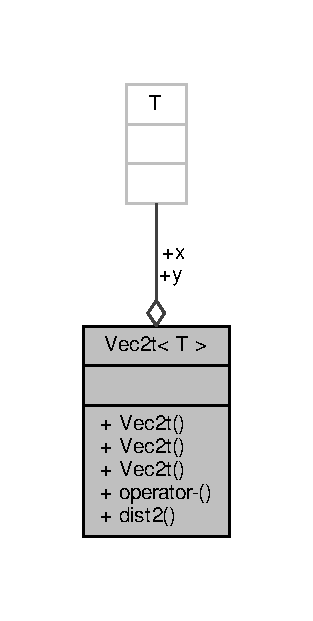
\includegraphics[width=150pt]{structVec2t__coll__graph}
\end{center}
\end{figure}
\subsection*{Public Member Functions}
\begin{DoxyCompactItemize}
\item 
\hyperlink{structVec2t_a6f9932f3a20db459c57d3be2d593a3a7}{Vec2t} ()
\item 
\hyperlink{structVec2t_a41fc85a32a9b215f05b9297c55528ff7}{Vec2t} (T \+\_\+x, T \+\_\+y)
\item 
{\footnotesize template$<$class T2 $>$ }\\\hyperlink{structVec2t_a4e9175daa9b5fa681594a409b2028a2e}{Vec2t} (const \hyperlink{structVec2t}{Vec2t}$<$ T2 $>$ \&rhs)
\item 
\hyperlink{structVec2t}{Vec2t} \hyperlink{structVec2t_a68504c899d03bf6fe08fd2581ec7bbb7}{operator-\/} () const 
\item 
T \hyperlink{structVec2t_a93ad4ffde1d4e300aa99565092df2d7b}{dist2} () const 
\end{DoxyCompactItemize}
\subsection*{Public Attributes}
\begin{DoxyCompactItemize}
\item 
T \hyperlink{structVec2t_a73d1b0cbfbbcf75d3dd534e75f9d32b1}{x}
\item 
T \hyperlink{structVec2t_a42162c3f5b97b3d1589feb70cae7834e}{y}
\end{DoxyCompactItemize}


\subsection{Constructor \& Destructor Documentation}
\index{Vec2t@{Vec2t}!Vec2t@{Vec2t}}
\index{Vec2t@{Vec2t}!Vec2t@{Vec2t}}
\subsubsection[{\texorpdfstring{Vec2t()}{Vec2t()}}]{\setlength{\rightskip}{0pt plus 5cm}template$<$class T$>$ {\bf Vec2t}$<$ T $>$\+::{\bf Vec2t} (
\begin{DoxyParamCaption}
{}
\end{DoxyParamCaption}
)\hspace{0.3cm}{\ttfamily [inline]}}\hypertarget{structVec2t_a6f9932f3a20db459c57d3be2d593a3a7}{}\label{structVec2t_a6f9932f3a20db459c57d3be2d593a3a7}
\index{Vec2t@{Vec2t}!Vec2t@{Vec2t}}
\index{Vec2t@{Vec2t}!Vec2t@{Vec2t}}
\subsubsection[{\texorpdfstring{Vec2t(\+T \+\_\+x, T \+\_\+y)}{Vec2t(T _x, T _y)}}]{\setlength{\rightskip}{0pt plus 5cm}template$<$class T$>$ {\bf Vec2t}$<$ T $>$\+::{\bf Vec2t} (
\begin{DoxyParamCaption}
\item[{T}]{\+\_\+x, }
\item[{T}]{\+\_\+y}
\end{DoxyParamCaption}
)\hspace{0.3cm}{\ttfamily [inline]}}\hypertarget{structVec2t_a41fc85a32a9b215f05b9297c55528ff7}{}\label{structVec2t_a41fc85a32a9b215f05b9297c55528ff7}
\index{Vec2t@{Vec2t}!Vec2t@{Vec2t}}
\index{Vec2t@{Vec2t}!Vec2t@{Vec2t}}
\subsubsection[{\texorpdfstring{Vec2t(const Vec2t$<$ T2 $>$ \&rhs)}{Vec2t(const Vec2t< T2 > &rhs)}}]{\setlength{\rightskip}{0pt plus 5cm}template$<$class T$>$ template$<$class T2 $>$ {\bf Vec2t}$<$ T $>$\+::{\bf Vec2t} (
\begin{DoxyParamCaption}
\item[{const {\bf Vec2t}$<$ T2 $>$ \&}]{rhs}
\end{DoxyParamCaption}
)\hspace{0.3cm}{\ttfamily [inline]}}\hypertarget{structVec2t_a4e9175daa9b5fa681594a409b2028a2e}{}\label{structVec2t_a4e9175daa9b5fa681594a409b2028a2e}


\subsection{Member Function Documentation}
\index{Vec2t@{Vec2t}!dist2@{dist2}}
\index{dist2@{dist2}!Vec2t@{Vec2t}}
\subsubsection[{\texorpdfstring{dist2() const }{dist2() const }}]{\setlength{\rightskip}{0pt plus 5cm}template$<$class T$>$ T {\bf Vec2t}$<$ T $>$\+::dist2 (
\begin{DoxyParamCaption}
{}
\end{DoxyParamCaption}
) const\hspace{0.3cm}{\ttfamily [inline]}}\hypertarget{structVec2t_a93ad4ffde1d4e300aa99565092df2d7b}{}\label{structVec2t_a93ad4ffde1d4e300aa99565092df2d7b}
\index{Vec2t@{Vec2t}!operator-\/@{operator-\/}}
\index{operator-\/@{operator-\/}!Vec2t@{Vec2t}}
\subsubsection[{\texorpdfstring{operator-\/() const }{operator-() const }}]{\setlength{\rightskip}{0pt plus 5cm}template$<$class T$>$ {\bf Vec2t} {\bf Vec2t}$<$ T $>$\+::operator-\/ (
\begin{DoxyParamCaption}
{}
\end{DoxyParamCaption}
) const\hspace{0.3cm}{\ttfamily [inline]}}\hypertarget{structVec2t_a68504c899d03bf6fe08fd2581ec7bbb7}{}\label{structVec2t_a68504c899d03bf6fe08fd2581ec7bbb7}


\subsection{Member Data Documentation}
\index{Vec2t@{Vec2t}!x@{x}}
\index{x@{x}!Vec2t@{Vec2t}}
\subsubsection[{\texorpdfstring{x}{x}}]{\setlength{\rightskip}{0pt plus 5cm}template$<$class T$>$ T {\bf Vec2t}$<$ T $>$\+::x}\hypertarget{structVec2t_a73d1b0cbfbbcf75d3dd534e75f9d32b1}{}\label{structVec2t_a73d1b0cbfbbcf75d3dd534e75f9d32b1}
\index{Vec2t@{Vec2t}!y@{y}}
\index{y@{y}!Vec2t@{Vec2t}}
\subsubsection[{\texorpdfstring{y}{y}}]{\setlength{\rightskip}{0pt plus 5cm}template$<$class T$>$ T {\bf Vec2t}$<$ T $>$\+::y}\hypertarget{structVec2t_a42162c3f5b97b3d1589feb70cae7834e}{}\label{structVec2t_a42162c3f5b97b3d1589feb70cae7834e}


The documentation for this struct was generated from the following file\+:\begin{DoxyCompactItemize}
\item 
\hyperlink{vec_8h}{vec.\+h}\end{DoxyCompactItemize}

\hypertarget{structVec3t}{}\section{Vec3t$<$ T $>$ Struct Template Reference}
\label{structVec3t}\index{Vec3t$<$ T $>$@{Vec3t$<$ T $>$}}


{\ttfamily \#include $<$vec.\+h$>$}



Collaboration diagram for Vec3t$<$ T $>$\+:\nopagebreak
\begin{figure}[H]
\begin{center}
\leavevmode
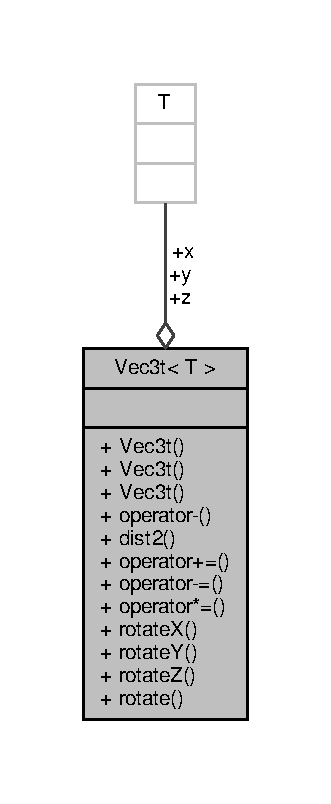
\includegraphics[width=159pt]{structVec3t__coll__graph}
\end{center}
\end{figure}
\subsection*{Public Member Functions}
\begin{DoxyCompactItemize}
\item 
\hyperlink{structVec3t_a7b34fabf25ecd175b48676c94e1d30e2}{Vec3t} ()
\item 
\hyperlink{structVec3t_a875345565deb7041f491007694069643}{Vec3t} (T \+\_\+x, T \+\_\+y, T \+\_\+z)
\item 
{\footnotesize template$<$class T2 $>$ }\\\hyperlink{structVec3t_aa0dc41bfc5a79373fbbd097d04424cb3}{Vec3t} (const \hyperlink{structVec3t}{Vec3t}$<$ T2 $>$ \&rhs)
\item 
\hyperlink{structVec3t}{Vec3t} \hyperlink{structVec3t_a038cd4e9b899cf7a49bea445981d2f25}{operator-\/} () const 
\item 
T \hyperlink{structVec3t_adc5afa9029b489909309fb6fa9f753f0}{dist2} () const 
\item 
\hyperlink{structVec3t}{Vec3t} \& \hyperlink{structVec3t_a4be2b3ccfcb0c7193141ad00877bb270}{operator+=} (const \hyperlink{structVec3t}{Vec3t} \&rhs)
\item 
\hyperlink{structVec3t}{Vec3t} \& \hyperlink{structVec3t_affe2466fb808a27bc15b507de3defcd0}{operator-\/=} (const \hyperlink{structVec3t}{Vec3t} \&rhs)
\item 
\hyperlink{structVec3t}{Vec3t} \& \hyperlink{structVec3t_a52a2a99aeaa3fba66c8d8efd566f1927}{operator$\ast$=} (T k)
\item 
\hyperlink{structVec3t}{Vec3t} \hyperlink{structVec3t_a95866fa2e01251b7a5920ce9d432341a}{rotateX} (T theta) const 
\begin{DoxyCompactList}\small\item\em Rotate around X-\/axis. \end{DoxyCompactList}\item 
\hyperlink{structVec3t}{Vec3t} \hyperlink{structVec3t_a66847d9c91164216e253359d7e12d6fe}{rotateY} (T theta) const 
\begin{DoxyCompactList}\small\item\em Rotate around Y-\/axis. \end{DoxyCompactList}\item 
\hyperlink{structVec3t}{Vec3t} \hyperlink{structVec3t_ac781f5660c197927efea3ade0b940dd3}{rotateZ} (T theta) const 
\begin{DoxyCompactList}\small\item\em Rotate around Z-\/axis. \end{DoxyCompactList}\item 
\hyperlink{structVec3t}{Vec3t} \hyperlink{structVec3t_a4dd2b7633407d6eec22ad24a222f9341}{rotate} (T phi, T theta) const 
\begin{DoxyCompactList}\small\item\em Skew theta angle with phi direction in a semisphere. \end{DoxyCompactList}\end{DoxyCompactItemize}
\subsection*{Public Attributes}
\begin{DoxyCompactItemize}
\item 
T \hyperlink{structVec3t_a71e5e9a4307fb9973fbbb189cdab6ece}{x}
\item 
T \hyperlink{structVec3t_a0dbe50be96dabd1d09c0866e1df61470}{y}
\item 
T \hyperlink{structVec3t_a9337e7d087c3a26e833de8c6fefca59b}{z}
\end{DoxyCompactItemize}


\subsection{Constructor \& Destructor Documentation}
\index{Vec3t@{Vec3t}!Vec3t@{Vec3t}}
\index{Vec3t@{Vec3t}!Vec3t@{Vec3t}}
\subsubsection[{\texorpdfstring{Vec3t()}{Vec3t()}}]{\setlength{\rightskip}{0pt plus 5cm}template$<$class T$>$ {\bf Vec3t}$<$ T $>$\+::{\bf Vec3t} (
\begin{DoxyParamCaption}
{}
\end{DoxyParamCaption}
)\hspace{0.3cm}{\ttfamily [inline]}}\hypertarget{structVec3t_a7b34fabf25ecd175b48676c94e1d30e2}{}\label{structVec3t_a7b34fabf25ecd175b48676c94e1d30e2}
\index{Vec3t@{Vec3t}!Vec3t@{Vec3t}}
\index{Vec3t@{Vec3t}!Vec3t@{Vec3t}}
\subsubsection[{\texorpdfstring{Vec3t(\+T \+\_\+x, T \+\_\+y, T \+\_\+z)}{Vec3t(T _x, T _y, T _z)}}]{\setlength{\rightskip}{0pt plus 5cm}template$<$class T$>$ {\bf Vec3t}$<$ T $>$\+::{\bf Vec3t} (
\begin{DoxyParamCaption}
\item[{T}]{\+\_\+x, }
\item[{T}]{\+\_\+y, }
\item[{T}]{\+\_\+z}
\end{DoxyParamCaption}
)\hspace{0.3cm}{\ttfamily [inline]}}\hypertarget{structVec3t_a875345565deb7041f491007694069643}{}\label{structVec3t_a875345565deb7041f491007694069643}
\index{Vec3t@{Vec3t}!Vec3t@{Vec3t}}
\index{Vec3t@{Vec3t}!Vec3t@{Vec3t}}
\subsubsection[{\texorpdfstring{Vec3t(const Vec3t$<$ T2 $>$ \&rhs)}{Vec3t(const Vec3t< T2 > &rhs)}}]{\setlength{\rightskip}{0pt plus 5cm}template$<$class T$>$ template$<$class T2 $>$ {\bf Vec3t}$<$ T $>$\+::{\bf Vec3t} (
\begin{DoxyParamCaption}
\item[{const {\bf Vec3t}$<$ T2 $>$ \&}]{rhs}
\end{DoxyParamCaption}
)\hspace{0.3cm}{\ttfamily [inline]}}\hypertarget{structVec3t_aa0dc41bfc5a79373fbbd097d04424cb3}{}\label{structVec3t_aa0dc41bfc5a79373fbbd097d04424cb3}


\subsection{Member Function Documentation}
\index{Vec3t@{Vec3t}!dist2@{dist2}}
\index{dist2@{dist2}!Vec3t@{Vec3t}}
\subsubsection[{\texorpdfstring{dist2() const }{dist2() const }}]{\setlength{\rightskip}{0pt plus 5cm}template$<$class T$>$ T {\bf Vec3t}$<$ T $>$\+::dist2 (
\begin{DoxyParamCaption}
{}
\end{DoxyParamCaption}
) const\hspace{0.3cm}{\ttfamily [inline]}}\hypertarget{structVec3t_adc5afa9029b489909309fb6fa9f753f0}{}\label{structVec3t_adc5afa9029b489909309fb6fa9f753f0}
\index{Vec3t@{Vec3t}!operator$\ast$=@{operator$\ast$=}}
\index{operator$\ast$=@{operator$\ast$=}!Vec3t@{Vec3t}}
\subsubsection[{\texorpdfstring{operator$\ast$=(\+T k)}{operator*=(T k)}}]{\setlength{\rightskip}{0pt plus 5cm}template$<$class T$>$ {\bf Vec3t}\& {\bf Vec3t}$<$ T $>$\+::operator$\ast$= (
\begin{DoxyParamCaption}
\item[{T}]{k}
\end{DoxyParamCaption}
)\hspace{0.3cm}{\ttfamily [inline]}}\hypertarget{structVec3t_a52a2a99aeaa3fba66c8d8efd566f1927}{}\label{structVec3t_a52a2a99aeaa3fba66c8d8efd566f1927}
\index{Vec3t@{Vec3t}!operator+=@{operator+=}}
\index{operator+=@{operator+=}!Vec3t@{Vec3t}}
\subsubsection[{\texorpdfstring{operator+=(const Vec3t \&rhs)}{operator+=(const Vec3t &rhs)}}]{\setlength{\rightskip}{0pt plus 5cm}template$<$class T$>$ {\bf Vec3t}\& {\bf Vec3t}$<$ T $>$\+::operator+= (
\begin{DoxyParamCaption}
\item[{const {\bf Vec3t}$<$ T $>$ \&}]{rhs}
\end{DoxyParamCaption}
)\hspace{0.3cm}{\ttfamily [inline]}}\hypertarget{structVec3t_a4be2b3ccfcb0c7193141ad00877bb270}{}\label{structVec3t_a4be2b3ccfcb0c7193141ad00877bb270}
\index{Vec3t@{Vec3t}!operator-\/@{operator-\/}}
\index{operator-\/@{operator-\/}!Vec3t@{Vec3t}}
\subsubsection[{\texorpdfstring{operator-\/() const }{operator-() const }}]{\setlength{\rightskip}{0pt plus 5cm}template$<$class T$>$ {\bf Vec3t} {\bf Vec3t}$<$ T $>$\+::operator-\/ (
\begin{DoxyParamCaption}
{}
\end{DoxyParamCaption}
) const\hspace{0.3cm}{\ttfamily [inline]}}\hypertarget{structVec3t_a038cd4e9b899cf7a49bea445981d2f25}{}\label{structVec3t_a038cd4e9b899cf7a49bea445981d2f25}
\index{Vec3t@{Vec3t}!operator-\/=@{operator-\/=}}
\index{operator-\/=@{operator-\/=}!Vec3t@{Vec3t}}
\subsubsection[{\texorpdfstring{operator-\/=(const Vec3t \&rhs)}{operator-=(const Vec3t &rhs)}}]{\setlength{\rightskip}{0pt plus 5cm}template$<$class T$>$ {\bf Vec3t}\& {\bf Vec3t}$<$ T $>$\+::operator-\/= (
\begin{DoxyParamCaption}
\item[{const {\bf Vec3t}$<$ T $>$ \&}]{rhs}
\end{DoxyParamCaption}
)\hspace{0.3cm}{\ttfamily [inline]}}\hypertarget{structVec3t_affe2466fb808a27bc15b507de3defcd0}{}\label{structVec3t_affe2466fb808a27bc15b507de3defcd0}
\index{Vec3t@{Vec3t}!rotate@{rotate}}
\index{rotate@{rotate}!Vec3t@{Vec3t}}
\subsubsection[{\texorpdfstring{rotate(\+T phi, T theta) const }{rotate(T phi, T theta) const }}]{\setlength{\rightskip}{0pt plus 5cm}template$<$class T$>$ {\bf Vec3t} {\bf Vec3t}$<$ T $>$\+::rotate (
\begin{DoxyParamCaption}
\item[{T}]{phi, }
\item[{T}]{theta}
\end{DoxyParamCaption}
) const\hspace{0.3cm}{\ttfamily [inline]}}\hypertarget{structVec3t_a4dd2b7633407d6eec22ad24a222f9341}{}\label{structVec3t_a4dd2b7633407d6eec22ad24a222f9341}


Skew theta angle with phi direction in a semisphere. 

\index{Vec3t@{Vec3t}!rotateX@{rotateX}}
\index{rotateX@{rotateX}!Vec3t@{Vec3t}}
\subsubsection[{\texorpdfstring{rotate\+X(\+T theta) const }{rotateX(T theta) const }}]{\setlength{\rightskip}{0pt plus 5cm}template$<$class T$>$ {\bf Vec3t} {\bf Vec3t}$<$ T $>$\+::rotateX (
\begin{DoxyParamCaption}
\item[{T}]{theta}
\end{DoxyParamCaption}
) const\hspace{0.3cm}{\ttfamily [inline]}}\hypertarget{structVec3t_a95866fa2e01251b7a5920ce9d432341a}{}\label{structVec3t_a95866fa2e01251b7a5920ce9d432341a}


Rotate around X-\/axis. 

\index{Vec3t@{Vec3t}!rotateY@{rotateY}}
\index{rotateY@{rotateY}!Vec3t@{Vec3t}}
\subsubsection[{\texorpdfstring{rotate\+Y(\+T theta) const }{rotateY(T theta) const }}]{\setlength{\rightskip}{0pt plus 5cm}template$<$class T$>$ {\bf Vec3t} {\bf Vec3t}$<$ T $>$\+::rotateY (
\begin{DoxyParamCaption}
\item[{T}]{theta}
\end{DoxyParamCaption}
) const\hspace{0.3cm}{\ttfamily [inline]}}\hypertarget{structVec3t_a66847d9c91164216e253359d7e12d6fe}{}\label{structVec3t_a66847d9c91164216e253359d7e12d6fe}


Rotate around Y-\/axis. 

\index{Vec3t@{Vec3t}!rotateZ@{rotateZ}}
\index{rotateZ@{rotateZ}!Vec3t@{Vec3t}}
\subsubsection[{\texorpdfstring{rotate\+Z(\+T theta) const }{rotateZ(T theta) const }}]{\setlength{\rightskip}{0pt plus 5cm}template$<$class T$>$ {\bf Vec3t} {\bf Vec3t}$<$ T $>$\+::rotateZ (
\begin{DoxyParamCaption}
\item[{T}]{theta}
\end{DoxyParamCaption}
) const\hspace{0.3cm}{\ttfamily [inline]}}\hypertarget{structVec3t_ac781f5660c197927efea3ade0b940dd3}{}\label{structVec3t_ac781f5660c197927efea3ade0b940dd3}


Rotate around Z-\/axis. 



\subsection{Member Data Documentation}
\index{Vec3t@{Vec3t}!x@{x}}
\index{x@{x}!Vec3t@{Vec3t}}
\subsubsection[{\texorpdfstring{x}{x}}]{\setlength{\rightskip}{0pt plus 5cm}template$<$class T$>$ T {\bf Vec3t}$<$ T $>$\+::x}\hypertarget{structVec3t_a71e5e9a4307fb9973fbbb189cdab6ece}{}\label{structVec3t_a71e5e9a4307fb9973fbbb189cdab6ece}
\index{Vec3t@{Vec3t}!y@{y}}
\index{y@{y}!Vec3t@{Vec3t}}
\subsubsection[{\texorpdfstring{y}{y}}]{\setlength{\rightskip}{0pt plus 5cm}template$<$class T$>$ T {\bf Vec3t}$<$ T $>$\+::y}\hypertarget{structVec3t_a0dbe50be96dabd1d09c0866e1df61470}{}\label{structVec3t_a0dbe50be96dabd1d09c0866e1df61470}
\index{Vec3t@{Vec3t}!z@{z}}
\index{z@{z}!Vec3t@{Vec3t}}
\subsubsection[{\texorpdfstring{z}{z}}]{\setlength{\rightskip}{0pt plus 5cm}template$<$class T$>$ T {\bf Vec3t}$<$ T $>$\+::z}\hypertarget{structVec3t_a9337e7d087c3a26e833de8c6fefca59b}{}\label{structVec3t_a9337e7d087c3a26e833de8c6fefca59b}


The documentation for this struct was generated from the following file\+:\begin{DoxyCompactItemize}
\item 
\hyperlink{vec_8h}{vec.\+h}\end{DoxyCompactItemize}

\chapter{File Documentation}
\hypertarget{axisymmetric_8h}{}\section{axisymmetric.\+h File Reference}
\label{axisymmetric_8h}\index{axisymmetric.\+h@{axisymmetric.\+h}}
{\ttfamily \#include $<$cassert$>$}\\*
{\ttfamily \#include $<$memory$>$}\\*
{\ttfamily \#include \char`\"{}../surface.\+h\char`\"{}}\\*
{\ttfamily \#include \char`\"{}../curve.\+h\char`\"{}}\\*
Include dependency graph for axisymmetric.\+h\+:\nopagebreak
\begin{figure}[H]
\begin{center}
\leavevmode
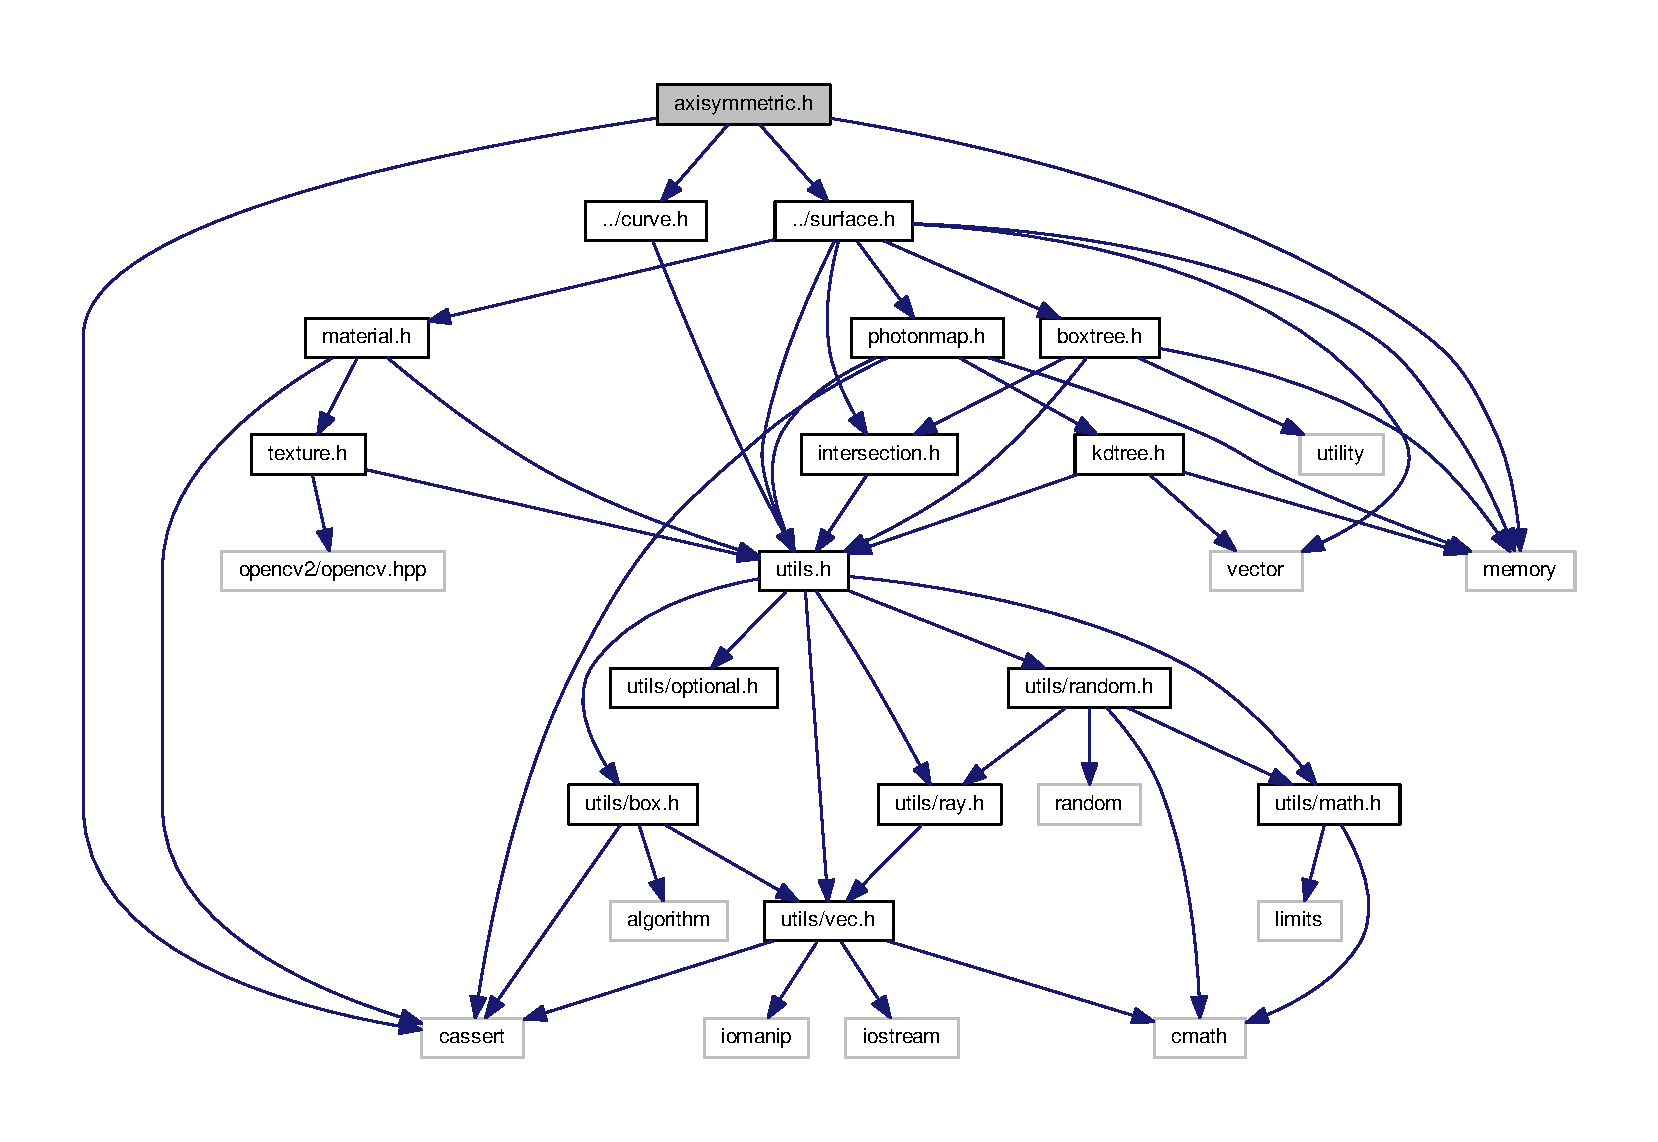
\includegraphics[width=350pt]{axisymmetric_8h__incl}
\end{center}
\end{figure}
This graph shows which files directly or indirectly include this file\+:\nopagebreak
\begin{figure}[H]
\begin{center}
\leavevmode
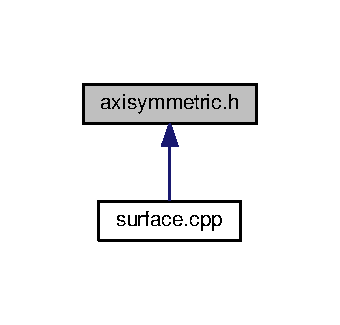
\includegraphics[width=163pt]{axisymmetric_8h__dep__incl}
\end{center}
\end{figure}
\subsection*{Classes}
\begin{DoxyCompactItemize}
\item 
class \hyperlink{classAxisymmetric}{Axisymmetric}
\begin{DoxyCompactList}\small\item\em Rotate a curve around z-\/axis to form a surface omega = u $\ast$ 2 $\ast$ PI, curve param = v \hyperlink{classCurve}{Curve(x, y)} =$>$ \hyperlink{classSurface}{Surface}(z, x $\sim$ y) If curve parameter v is positively correlated with x, normal goes outwards. \end{DoxyCompactList}\end{DoxyCompactItemize}

\hypertarget{bezier3_8h}{}\section{bezier3.\+h File Reference}
\label{bezier3_8h}\index{bezier3.\+h@{bezier3.\+h}}
{\ttfamily \#include $<$cmath$>$}\\*
{\ttfamily \#include $<$cassert$>$}\\*
{\ttfamily \#include \char`\"{}../curve.\+h\char`\"{}}\\*
{\ttfamily \#include \char`\"{}../const.\+h\char`\"{}}\\*
Include dependency graph for bezier3.\+h\+:\nopagebreak
\begin{figure}[H]
\begin{center}
\leavevmode
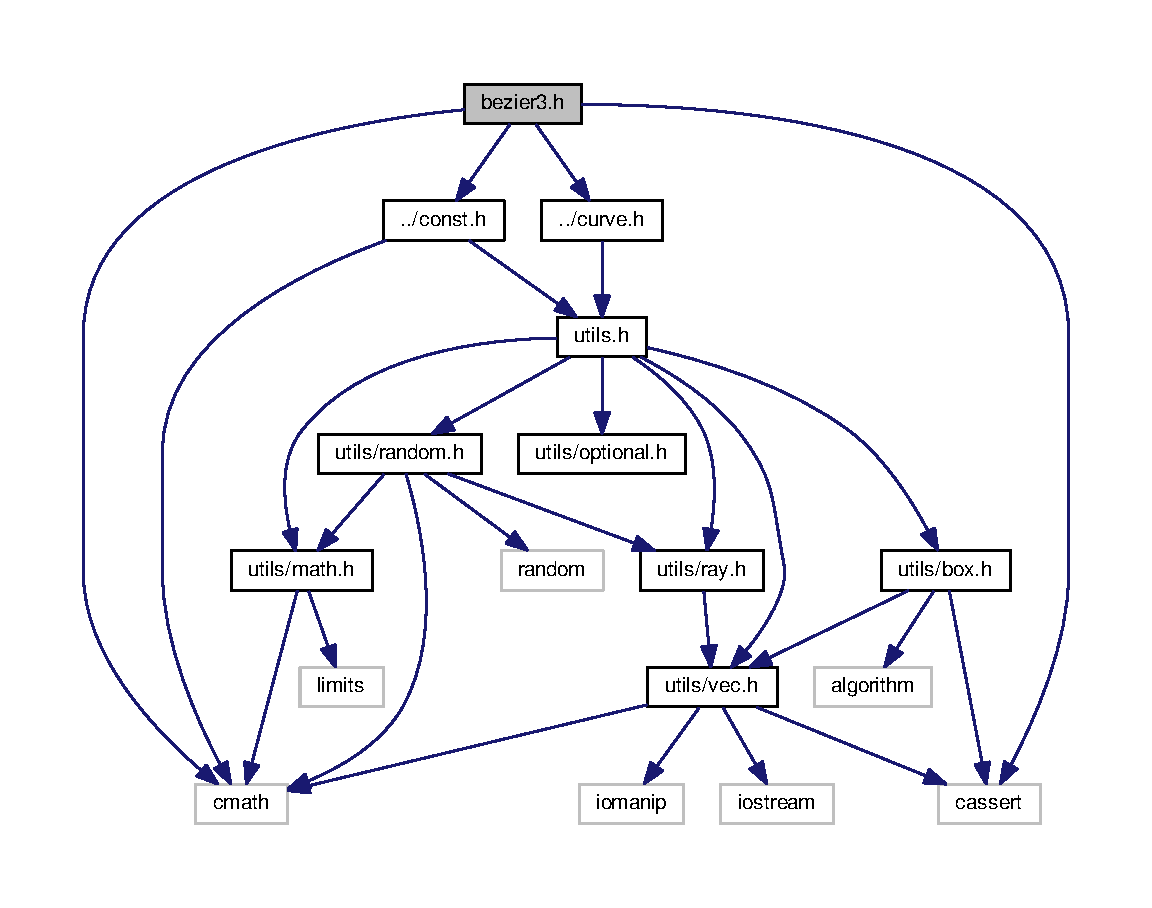
\includegraphics[width=350pt]{bezier3_8h__incl}
\end{center}
\end{figure}
This graph shows which files directly or indirectly include this file\+:\nopagebreak
\begin{figure}[H]
\begin{center}
\leavevmode
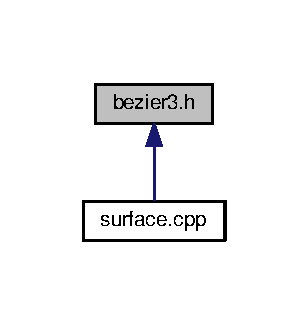
\includegraphics[width=148pt]{bezier3_8h__dep__incl}
\end{center}
\end{figure}
\subsection*{Classes}
\begin{DoxyCompactItemize}
\item 
class \hyperlink{classBezier3}{Bezier3}
\begin{DoxyCompactList}\small\item\em 3-\/dgree Bezier \hyperlink{classCurve}{Curve} \end{DoxyCompactList}\end{DoxyCompactItemize}

\hypertarget{box_8h}{}\section{box.\+h File Reference}
\label{box_8h}\index{box.\+h@{box.\+h}}
{\ttfamily \#include $<$cassert$>$}\\*
{\ttfamily \#include $<$algorithm$>$}\\*
{\ttfamily \#include \char`\"{}vec.\+h\char`\"{}}\\*
Include dependency graph for box.\+h\+:
\nopagebreak
\begin{figure}[H]
\begin{center}
\leavevmode
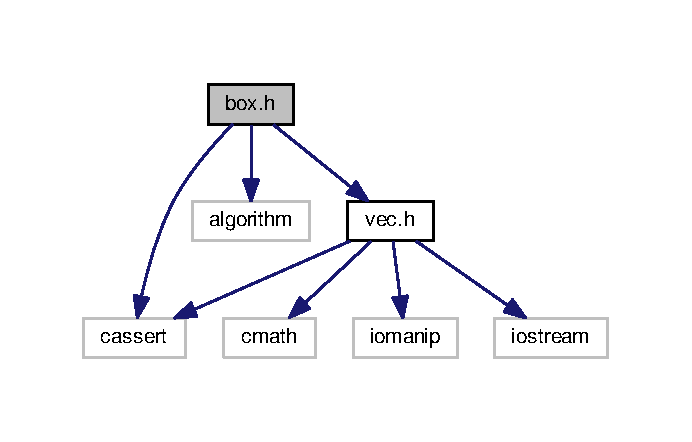
\includegraphics[width=332pt]{box_8h__incl}
\end{center}
\end{figure}
This graph shows which files directly or indirectly include this file\+:
\nopagebreak
\begin{figure}[H]
\begin{center}
\leavevmode
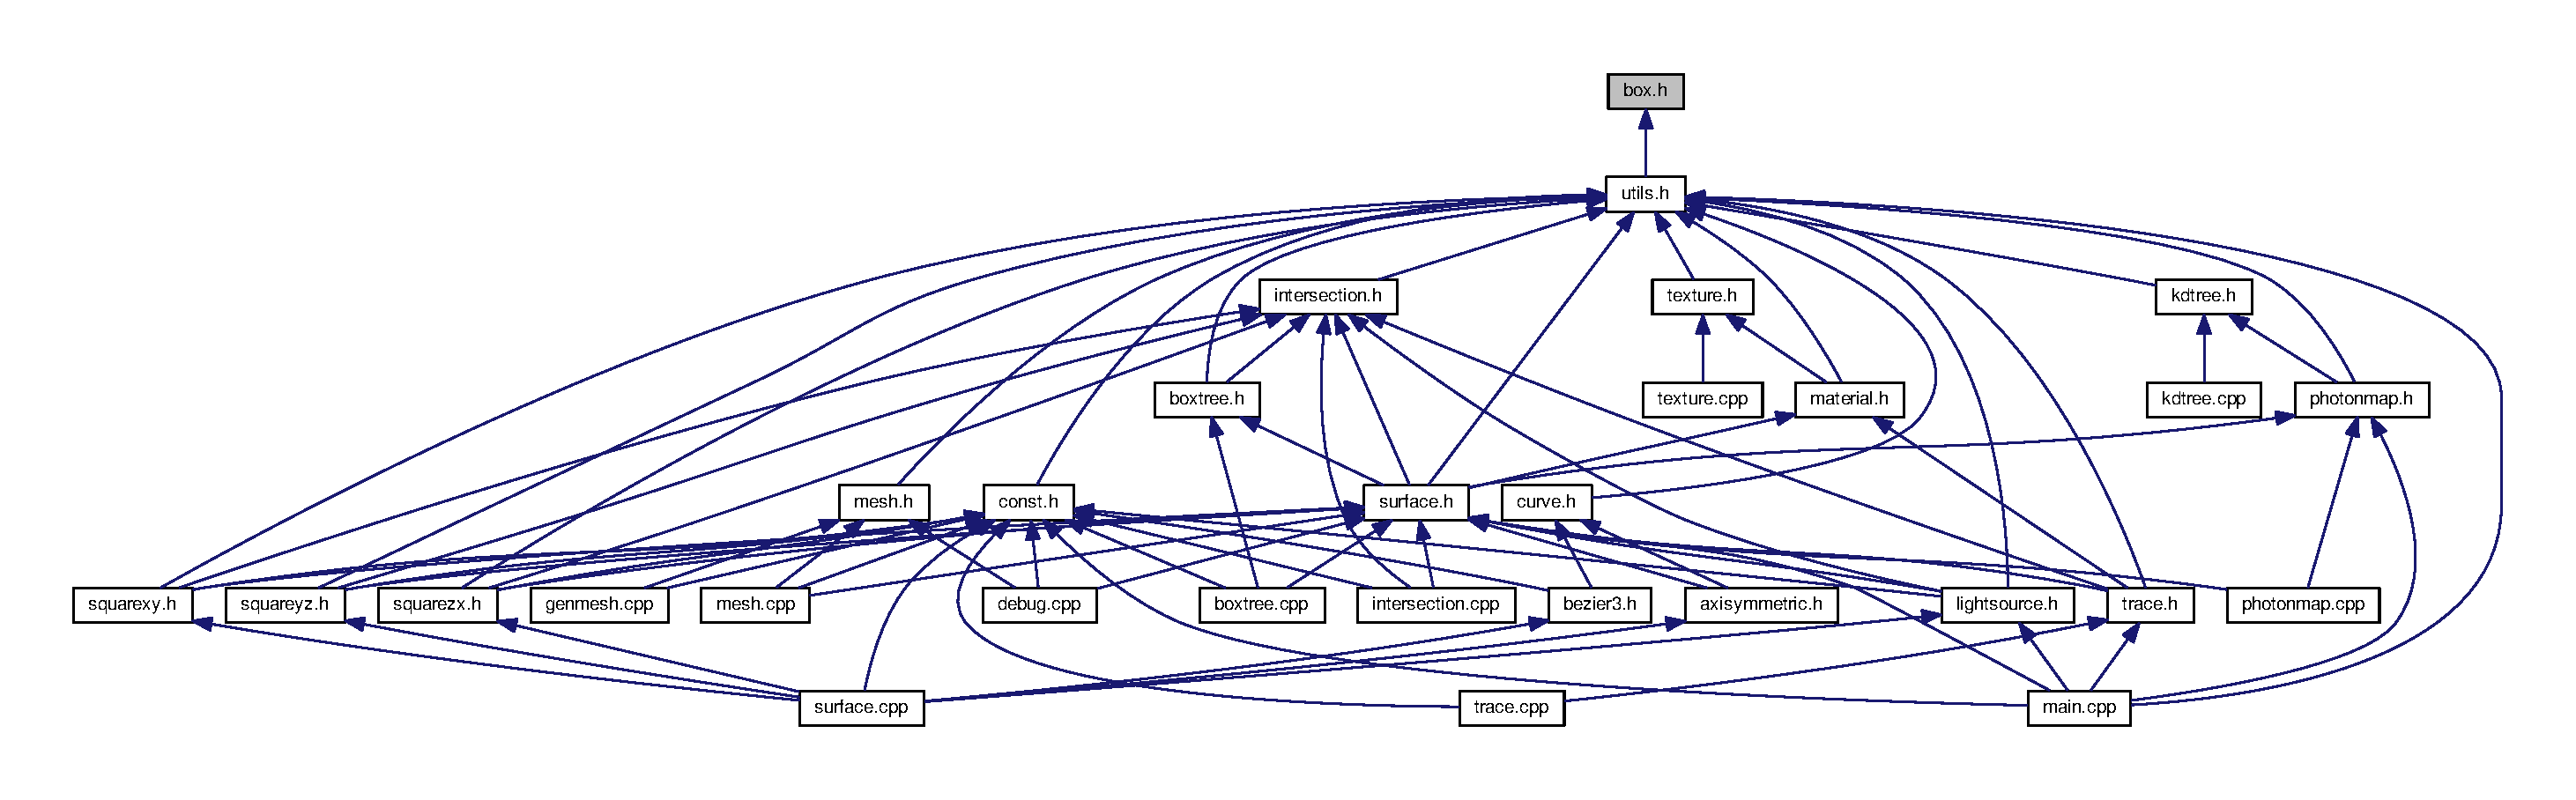
\includegraphics[width=350pt]{box_8h__dep__incl}
\end{center}
\end{figure}
\subsection*{Classes}
\begin{DoxyCompactItemize}
\item 
struct \hyperlink{structBox2}{Box2}
\item 
struct \hyperlink{structBox3}{Box3}
\end{DoxyCompactItemize}
\subsection*{Functions}
\begin{DoxyCompactItemize}
\item 
\hyperlink{structBox3}{Box3} \hyperlink{box_8h_a1b3a10f0b934f9887f264c795d5d202c}{merge} (const \hyperlink{structBox3}{Box3} \&lhs, const \hyperlink{structBox3}{Box3} \&rhs)
\end{DoxyCompactItemize}
\subsection*{Variables}
\begin{DoxyCompactItemize}
\item 
const float \hyperlink{box_8h_a3414d95e3edaf6d6c7d50f3ec59d8726}{B\+O\+X\+\_\+\+E\+PS} = 1e-\/3
\end{DoxyCompactItemize}


\subsection{Function Documentation}
\index{box.\+h@{box.\+h}!merge@{merge}}
\index{merge@{merge}!box.\+h@{box.\+h}}
\subsubsection[{\texorpdfstring{merge(const Box3 \&lhs, const Box3 \&rhs)}{merge(const Box3 &lhs, const Box3 &rhs)}}]{\setlength{\rightskip}{0pt plus 5cm}{\bf Box3} merge (
\begin{DoxyParamCaption}
\item[{const {\bf Box3} \&}]{lhs, }
\item[{const {\bf Box3} \&}]{rhs}
\end{DoxyParamCaption}
)\hspace{0.3cm}{\ttfamily [inline]}}\hypertarget{box_8h_a1b3a10f0b934f9887f264c795d5d202c}{}\label{box_8h_a1b3a10f0b934f9887f264c795d5d202c}


\subsection{Variable Documentation}
\index{box.\+h@{box.\+h}!B\+O\+X\+\_\+\+E\+PS@{B\+O\+X\+\_\+\+E\+PS}}
\index{B\+O\+X\+\_\+\+E\+PS@{B\+O\+X\+\_\+\+E\+PS}!box.\+h@{box.\+h}}
\subsubsection[{\texorpdfstring{B\+O\+X\+\_\+\+E\+PS}{BOX_EPS}}]{\setlength{\rightskip}{0pt plus 5cm}const float B\+O\+X\+\_\+\+E\+PS = 1e-\/3}\hypertarget{box_8h_a3414d95e3edaf6d6c7d50f3ec59d8726}{}\label{box_8h_a3414d95e3edaf6d6c7d50f3ec59d8726}

\hypertarget{boxtree_8cpp}{}\section{boxtree.\+cpp File Reference}
\label{boxtree_8cpp}\index{boxtree.\+cpp@{boxtree.\+cpp}}
{\ttfamily \#include $<$cassert$>$}\\*
{\ttfamily \#include \char`\"{}const.\+h\char`\"{}}\\*
{\ttfamily \#include \char`\"{}surface.\+h\char`\"{}}\\*
{\ttfamily \#include \char`\"{}boxtree.\+h\char`\"{}}\\*
Include dependency graph for boxtree.\+cpp\+:
\nopagebreak
\begin{figure}[H]
\begin{center}
\leavevmode
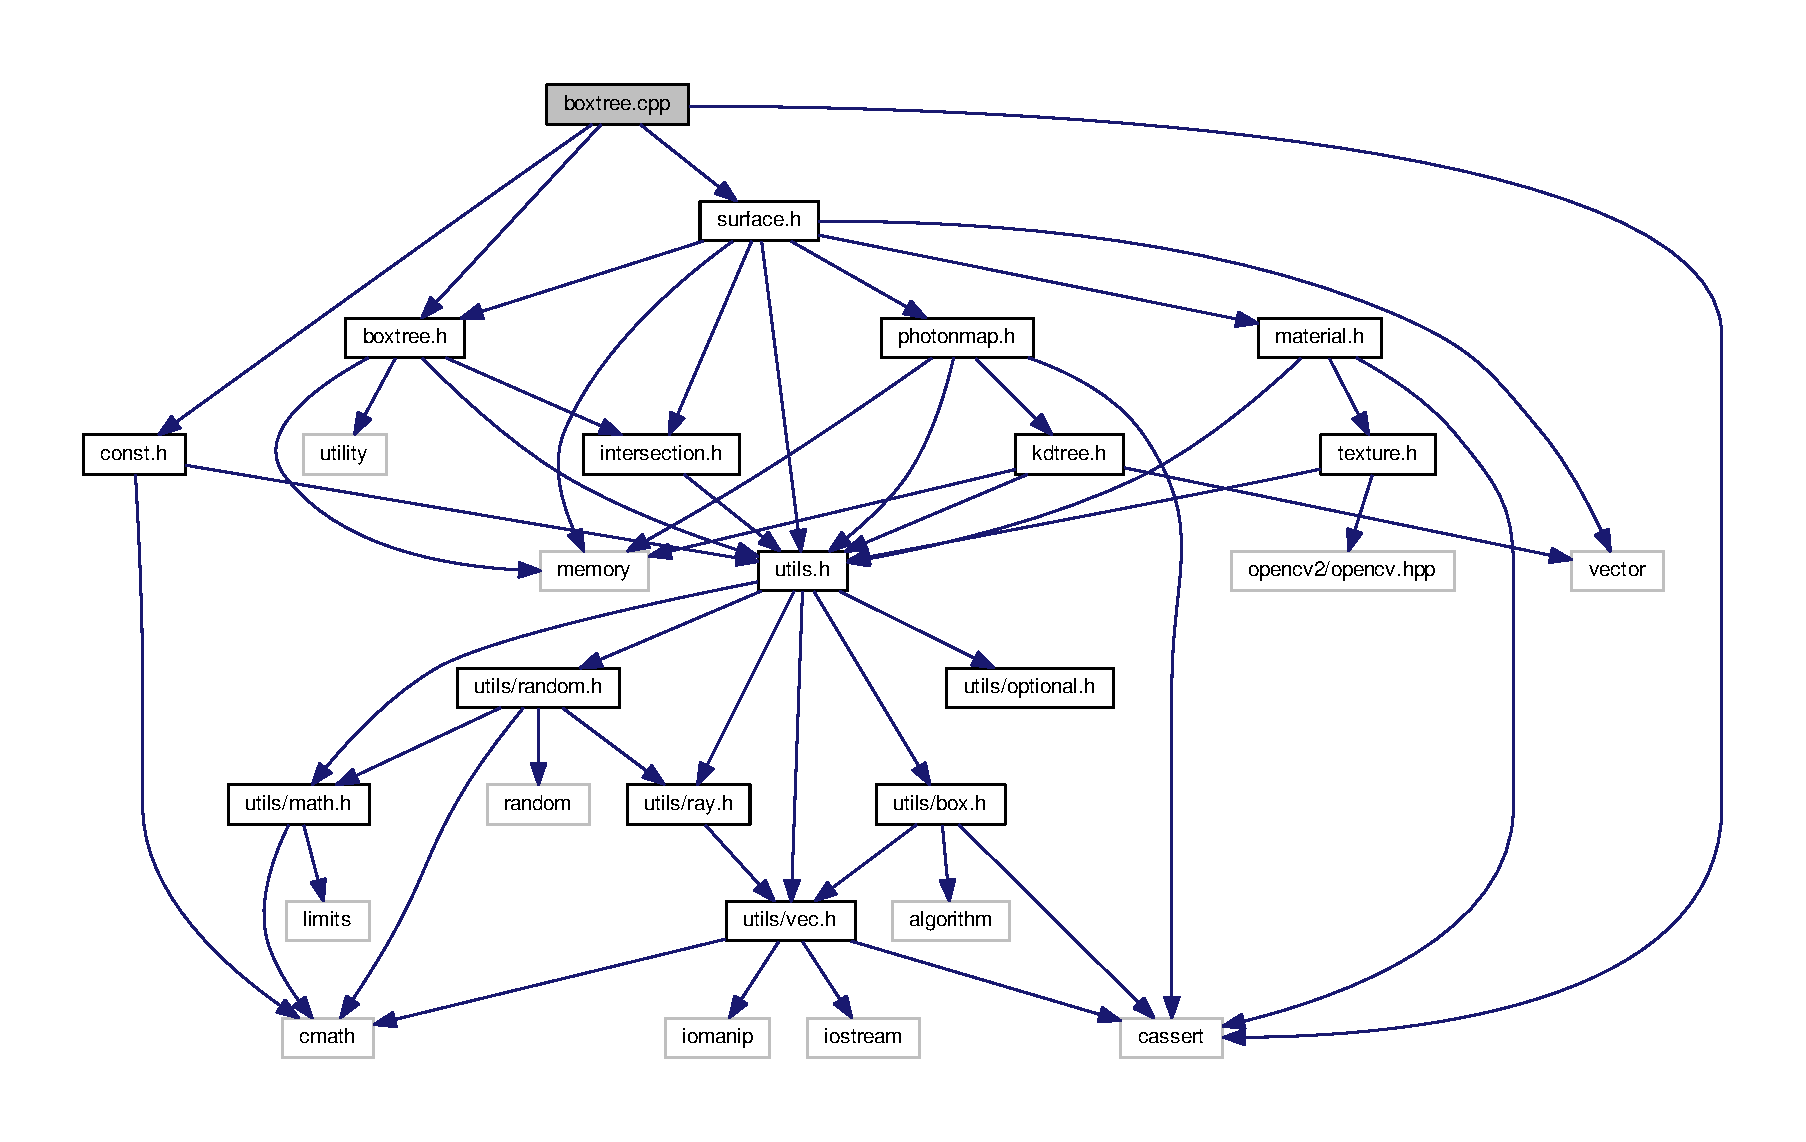
\includegraphics[width=350pt]{boxtree_8cpp__incl}
\end{center}
\end{figure}

\hypertarget{boxtree_8h}{}\section{boxtree.\+h File Reference}
\label{boxtree_8h}\index{boxtree.\+h@{boxtree.\+h}}
{\ttfamily \#include $<$memory$>$}\\*
{\ttfamily \#include $<$utility$>$}\\*
{\ttfamily \#include \char`\"{}utils.\+h\char`\"{}}\\*
{\ttfamily \#include \char`\"{}intersection.\+h\char`\"{}}\\*
Include dependency graph for boxtree.\+h\+:
\nopagebreak
\begin{figure}[H]
\begin{center}
\leavevmode
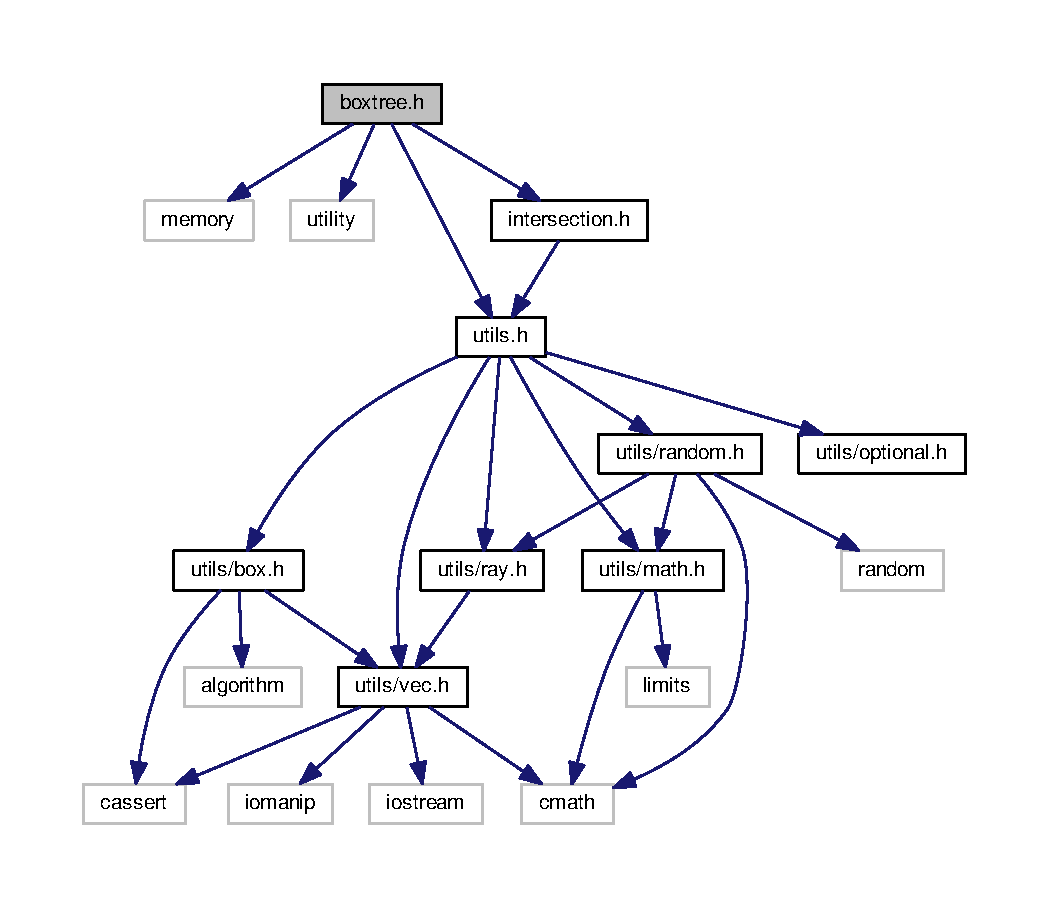
\includegraphics[width=350pt]{boxtree_8h__incl}
\end{center}
\end{figure}
This graph shows which files directly or indirectly include this file\+:
\nopagebreak
\begin{figure}[H]
\begin{center}
\leavevmode
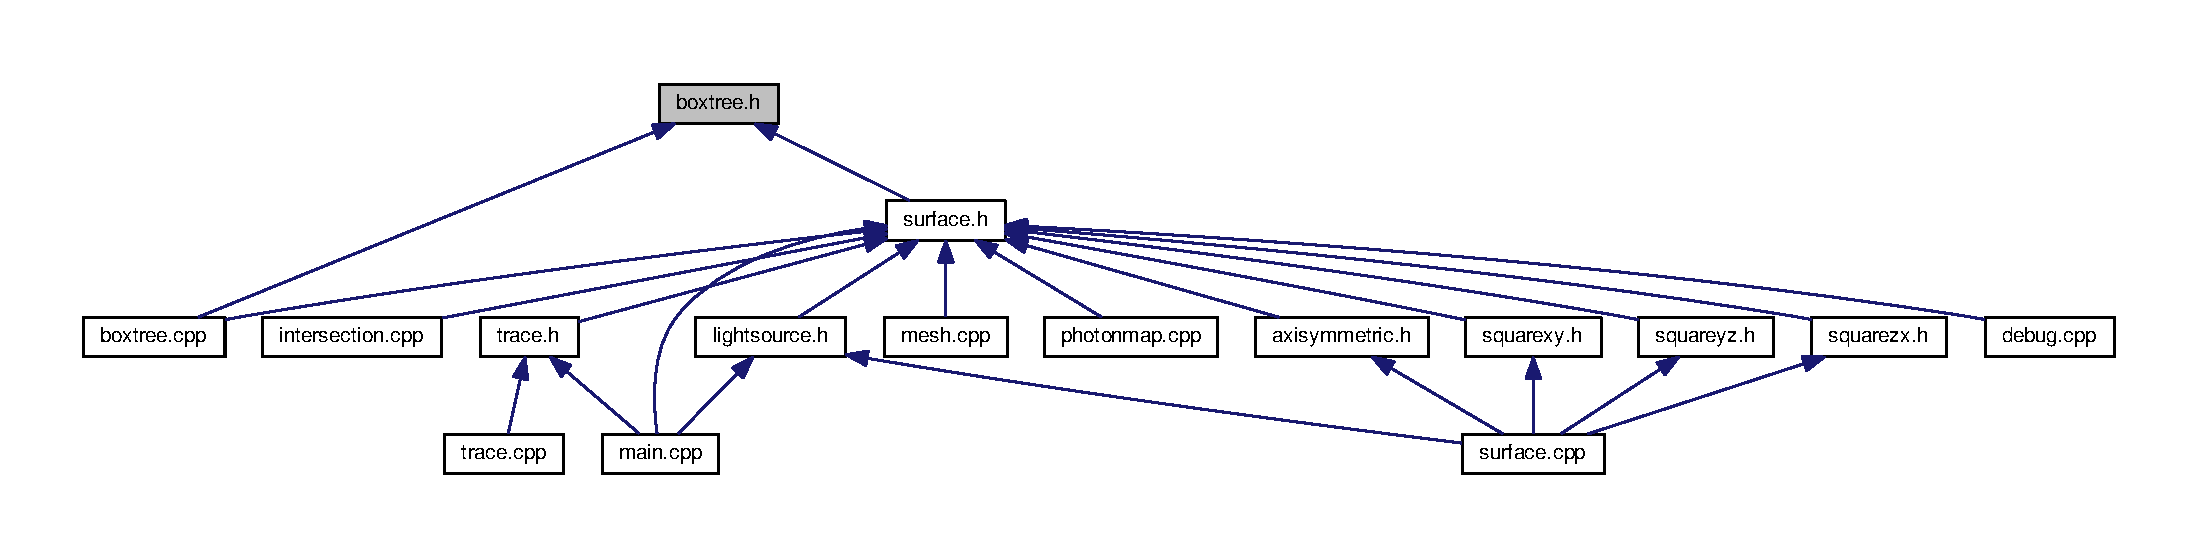
\includegraphics[width=350pt]{boxtree_8h__dep__incl}
\end{center}
\end{figure}
\subsection*{Classes}
\begin{DoxyCompactItemize}
\item 
class \hyperlink{classBoxTree}{Box\+Tree}
\begin{DoxyCompactList}\small\item\em Tree of bounding box built on a surface Organized by surface parameters (u, v) \end{DoxyCompactList}\item 
struct \hyperlink{structBoxTree_1_1Node}{Box\+Tree\+::\+Node}
\end{DoxyCompactItemize}

\hypertarget{const_8h}{}\section{const.\+h File Reference}
\label{const_8h}\index{const.\+h@{const.\+h}}
{\ttfamily \#include $<$cmath$>$}\\*
{\ttfamily \#include \char`\"{}utils.\+h\char`\"{}}\\*
Include dependency graph for const.\+h\+:\nopagebreak
\begin{figure}[H]
\begin{center}
\leavevmode
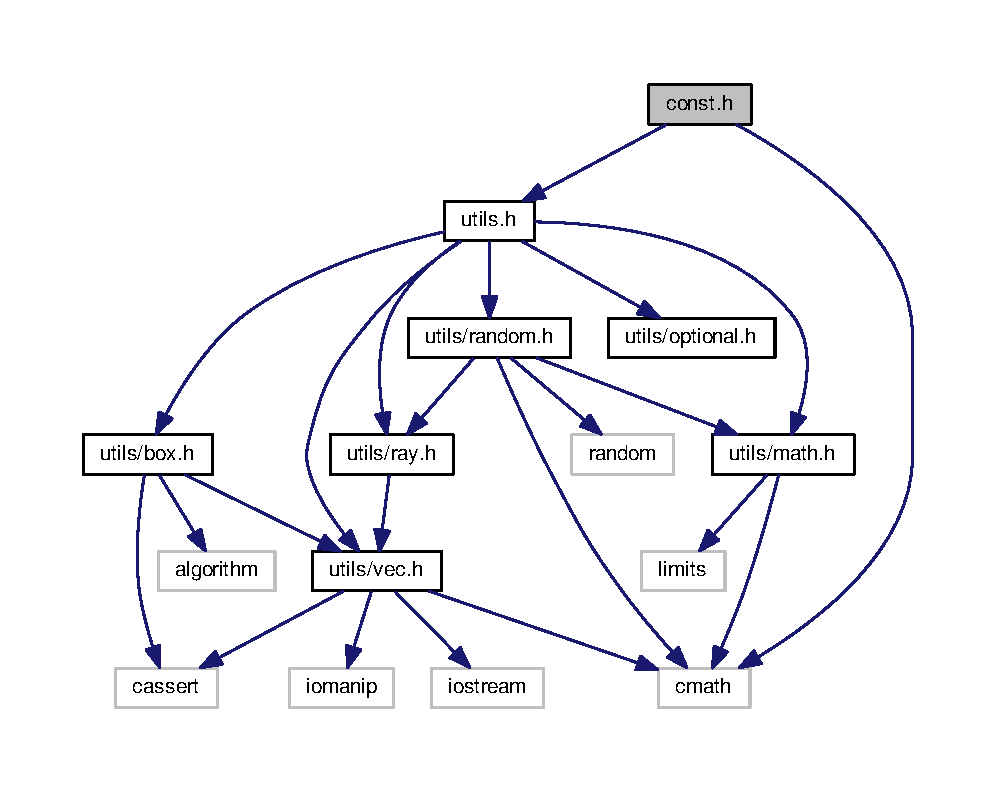
\includegraphics[width=350pt]{const_8h__incl}
\end{center}
\end{figure}
This graph shows which files directly or indirectly include this file\+:\nopagebreak
\begin{figure}[H]
\begin{center}
\leavevmode
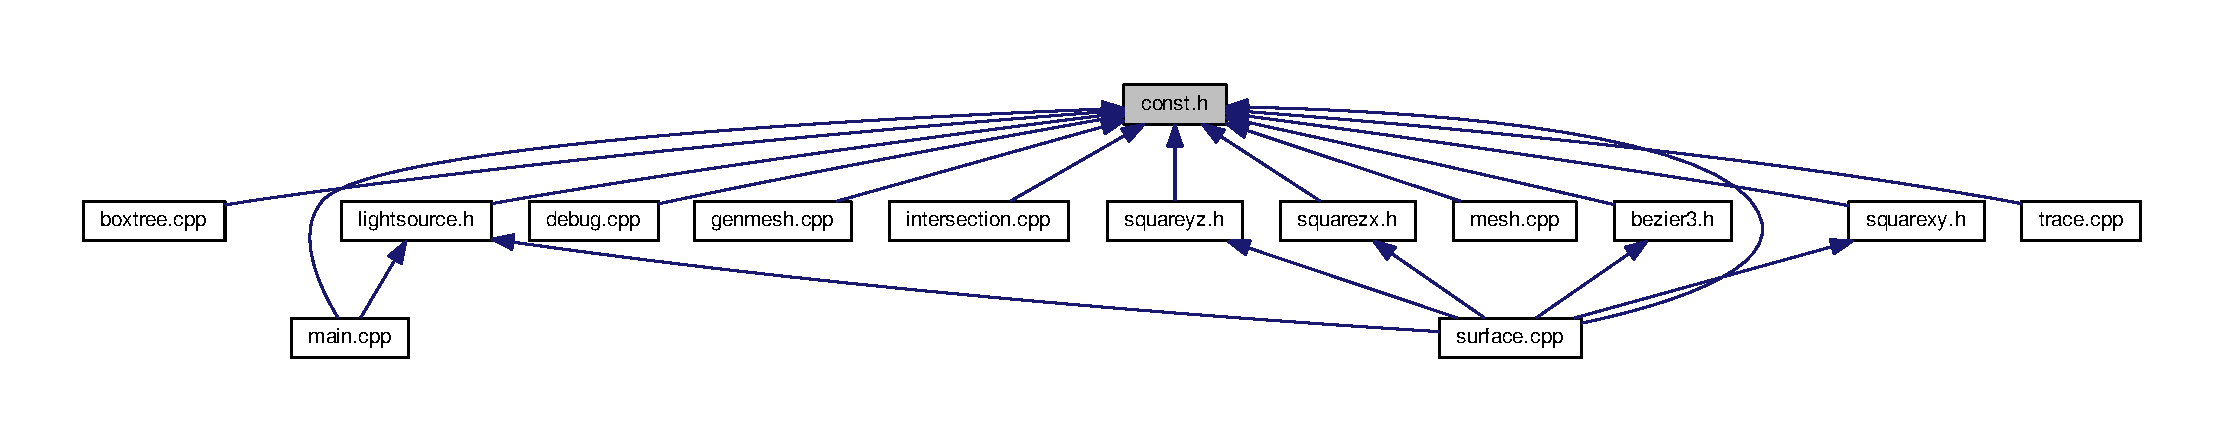
\includegraphics[width=350pt]{const_8h__dep__incl}
\end{center}
\end{figure}
\subsection*{Variables}
\begin{DoxyCompactItemize}
\item 
const char \hyperlink{const_8h_aecde119e346ac18d9583a635e6b6bd52}{I\+N\+P\+U\+T\+\_\+\+O\+B\+J\+E\+C\+T\+S\+\_\+\+F\+I\+LE} \mbox{[}$\,$\mbox{]} = \char`\"{}objects.\+txt\char`\"{}
\item 
const char \hyperlink{const_8h_a453112ff6ac02a238ba9ddea1ec99f81}{O\+U\+T\+P\+U\+T\+\_\+\+F\+I\+LE} \mbox{[}$\,$\mbox{]} = \char`\"{}output.\+png\char`\"{}
\item 
const char \hyperlink{const_8h_af99449ec4514a9a8de0c0ca36f66c353}{M\+E\+S\+H\+\_\+\+F\+I\+LE} \mbox{[}$\,$\mbox{]} = \char`\"{}mesh.\+obj\char`\"{}
\item 
const int \hyperlink{const_8h_afcd938c28b4d4d75d968883fb9273cda}{M\+E\+S\+H\+\_\+1\+D\+\_\+\+N\+UM} = 25
\item 
const int \hyperlink{const_8h_ad004486df64e99553ffc6d28f48035e1}{O\+U\+T\+P\+U\+T\+\_\+\+M\+E\+S\+H\+\_\+1\+D\+\_\+\+N\+UM} = 100
\item 
const float \hyperlink{const_8h_a8699e9cea9e8bd0b1b3a3bb7d6cf671c}{E\+PS} = 1e-\/3
\item 
const int \hyperlink{const_8h_a3482785bd2a4c8b307f9e0b6f54e2c36}{S\+C\+R\+E\+E\+N\+\_\+\+W\+I\+D\+TH} = 1024
\item 
const int \hyperlink{const_8h_ab454541ae58bcf6555e8d723b1eb95e7}{S\+C\+R\+E\+E\+N\+\_\+\+H\+E\+I\+G\+HT} = 768
\item 
const int \hyperlink{const_8h_aa88c9de2363556df02099d7ccc83ac4d}{D\+E\+P\+T\+H\+\_\+\+P\+E\+R\+\_\+\+L\+I\+G\+HT} = 5
\item 
const int \hyperlink{const_8h_a655c5b3882e191b283e9c1c2917d0223}{R\+A\+Y\+\_\+\+P\+E\+R\+\_\+\+L\+I\+G\+HT} = 10000000
\item 
const int \hyperlink{const_8h_a6fda20c9b4ebad0906984495de901073}{D\+E\+P\+T\+H\+\_\+\+P\+E\+R\+\_\+\+P\+I\+X\+EL} = 5
\item 
const int \hyperlink{const_8h_ab53b5a6f55f49097e95de28c4ea73994}{R\+A\+Y\+\_\+\+P\+E\+R\+\_\+\+P\+I\+X\+EL} = 250
\item 
const int \hyperlink{const_8h_a7fd37c1a0eb3d24ad2de161e3fb99840}{K\+N\+N\+\_\+K} = 100
\item 
constexpr const float \hyperlink{const_8h_a12f762a0aa13ec1a71dba1ce4f7be788}{L\+E\+N\+S\+\_\+Y} = -\/750
\item 
constexpr const float \hyperlink{const_8h_a9cf011c3467e5525ab5c6c3cc27bb414}{L\+E\+N\+S\+\_\+F} = 400
\item 
constexpr const float \hyperlink{const_8h_a699f799089a6c383d4edb95ada181577}{L\+E\+N\+S\+\_\+H} = \hyperlink{const_8h_a9cf011c3467e5525ab5c6c3cc27bb414}{L\+E\+N\+S\+\_\+F} / 9 / 2
\item 
constexpr const float \hyperlink{const_8h_a926bb03ef827da42216d105c5d89da35}{L\+E\+N\+S\+\_\+\+D2} = 700
\begin{DoxyCompactList}\small\item\em Aperture (diameter) / 2. \end{DoxyCompactList}\item 
constexpr const float \hyperlink{const_8h_ac918ff5a774282b2df5705bcce86e63b}{L\+E\+N\+S\+\_\+\+D1} = \hyperlink{const_8h_a926bb03ef827da42216d105c5d89da35}{L\+E\+N\+S\+\_\+\+D2} $\ast$ \hyperlink{const_8h_a9cf011c3467e5525ab5c6c3cc27bb414}{L\+E\+N\+S\+\_\+F} / (\hyperlink{const_8h_a926bb03ef827da42216d105c5d89da35}{L\+E\+N\+S\+\_\+\+D2} -\/ \hyperlink{const_8h_a9cf011c3467e5525ab5c6c3cc27bb414}{L\+E\+N\+S\+\_\+F})
\item 
constexpr const float \hyperlink{const_8h_a94830ff442bc6224792ab0f350fec4bc}{F\+I\+L\+M\+\_\+\+W\+I\+D\+TH} = 266.\+5 / (-\/266.\+5 -\/ \hyperlink{const_8h_a12f762a0aa13ec1a71dba1ce4f7be788}{L\+E\+N\+S\+\_\+Y}) $\ast$ \hyperlink{const_8h_ac918ff5a774282b2df5705bcce86e63b}{L\+E\+N\+S\+\_\+\+D1}
\item 
constexpr const float \hyperlink{const_8h_a73afd160beb2a236d3a66b82ffcb7bb8}{F\+I\+L\+M\+\_\+\+H\+E\+I\+G\+HT} = \hyperlink{const_8h_a94830ff442bc6224792ab0f350fec4bc}{F\+I\+L\+M\+\_\+\+W\+I\+D\+TH} / \hyperlink{const_8h_a3482785bd2a4c8b307f9e0b6f54e2c36}{S\+C\+R\+E\+E\+N\+\_\+\+W\+I\+D\+TH} $\ast$ \hyperlink{const_8h_ab454541ae58bcf6555e8d723b1eb95e7}{S\+C\+R\+E\+E\+N\+\_\+\+H\+E\+I\+G\+HT}
\end{DoxyCompactItemize}


\subsection{Variable Documentation}
\index{const.\+h@{const.\+h}!D\+E\+P\+T\+H\+\_\+\+P\+E\+R\+\_\+\+L\+I\+G\+HT@{D\+E\+P\+T\+H\+\_\+\+P\+E\+R\+\_\+\+L\+I\+G\+HT}}
\index{D\+E\+P\+T\+H\+\_\+\+P\+E\+R\+\_\+\+L\+I\+G\+HT@{D\+E\+P\+T\+H\+\_\+\+P\+E\+R\+\_\+\+L\+I\+G\+HT}!const.\+h@{const.\+h}}
\subsubsection[{\texorpdfstring{D\+E\+P\+T\+H\+\_\+\+P\+E\+R\+\_\+\+L\+I\+G\+HT}{DEPTH_PER_LIGHT}}]{\setlength{\rightskip}{0pt plus 5cm}const int D\+E\+P\+T\+H\+\_\+\+P\+E\+R\+\_\+\+L\+I\+G\+HT = 5}\hypertarget{const_8h_aa88c9de2363556df02099d7ccc83ac4d}{}\label{const_8h_aa88c9de2363556df02099d7ccc83ac4d}
\index{const.\+h@{const.\+h}!D\+E\+P\+T\+H\+\_\+\+P\+E\+R\+\_\+\+P\+I\+X\+EL@{D\+E\+P\+T\+H\+\_\+\+P\+E\+R\+\_\+\+P\+I\+X\+EL}}
\index{D\+E\+P\+T\+H\+\_\+\+P\+E\+R\+\_\+\+P\+I\+X\+EL@{D\+E\+P\+T\+H\+\_\+\+P\+E\+R\+\_\+\+P\+I\+X\+EL}!const.\+h@{const.\+h}}
\subsubsection[{\texorpdfstring{D\+E\+P\+T\+H\+\_\+\+P\+E\+R\+\_\+\+P\+I\+X\+EL}{DEPTH_PER_PIXEL}}]{\setlength{\rightskip}{0pt plus 5cm}const int D\+E\+P\+T\+H\+\_\+\+P\+E\+R\+\_\+\+P\+I\+X\+EL = 5}\hypertarget{const_8h_a6fda20c9b4ebad0906984495de901073}{}\label{const_8h_a6fda20c9b4ebad0906984495de901073}
\index{const.\+h@{const.\+h}!E\+PS@{E\+PS}}
\index{E\+PS@{E\+PS}!const.\+h@{const.\+h}}
\subsubsection[{\texorpdfstring{E\+PS}{EPS}}]{\setlength{\rightskip}{0pt plus 5cm}const float E\+PS = 1e-\/3}\hypertarget{const_8h_a8699e9cea9e8bd0b1b3a3bb7d6cf671c}{}\label{const_8h_a8699e9cea9e8bd0b1b3a3bb7d6cf671c}
\index{const.\+h@{const.\+h}!F\+I\+L\+M\+\_\+\+H\+E\+I\+G\+HT@{F\+I\+L\+M\+\_\+\+H\+E\+I\+G\+HT}}
\index{F\+I\+L\+M\+\_\+\+H\+E\+I\+G\+HT@{F\+I\+L\+M\+\_\+\+H\+E\+I\+G\+HT}!const.\+h@{const.\+h}}
\subsubsection[{\texorpdfstring{F\+I\+L\+M\+\_\+\+H\+E\+I\+G\+HT}{FILM_HEIGHT}}]{\setlength{\rightskip}{0pt plus 5cm}constexpr const float F\+I\+L\+M\+\_\+\+H\+E\+I\+G\+HT = {\bf F\+I\+L\+M\+\_\+\+W\+I\+D\+TH} / {\bf S\+C\+R\+E\+E\+N\+\_\+\+W\+I\+D\+TH} $\ast$ {\bf S\+C\+R\+E\+E\+N\+\_\+\+H\+E\+I\+G\+HT}}\hypertarget{const_8h_a73afd160beb2a236d3a66b82ffcb7bb8}{}\label{const_8h_a73afd160beb2a236d3a66b82ffcb7bb8}
\index{const.\+h@{const.\+h}!F\+I\+L\+M\+\_\+\+W\+I\+D\+TH@{F\+I\+L\+M\+\_\+\+W\+I\+D\+TH}}
\index{F\+I\+L\+M\+\_\+\+W\+I\+D\+TH@{F\+I\+L\+M\+\_\+\+W\+I\+D\+TH}!const.\+h@{const.\+h}}
\subsubsection[{\texorpdfstring{F\+I\+L\+M\+\_\+\+W\+I\+D\+TH}{FILM_WIDTH}}]{\setlength{\rightskip}{0pt plus 5cm}constexpr const float F\+I\+L\+M\+\_\+\+W\+I\+D\+TH = 266.\+5 / (-\/266.\+5 -\/ {\bf L\+E\+N\+S\+\_\+Y}) $\ast$ {\bf L\+E\+N\+S\+\_\+\+D1}}\hypertarget{const_8h_a94830ff442bc6224792ab0f350fec4bc}{}\label{const_8h_a94830ff442bc6224792ab0f350fec4bc}
\index{const.\+h@{const.\+h}!I\+N\+P\+U\+T\+\_\+\+O\+B\+J\+E\+C\+T\+S\+\_\+\+F\+I\+LE@{I\+N\+P\+U\+T\+\_\+\+O\+B\+J\+E\+C\+T\+S\+\_\+\+F\+I\+LE}}
\index{I\+N\+P\+U\+T\+\_\+\+O\+B\+J\+E\+C\+T\+S\+\_\+\+F\+I\+LE@{I\+N\+P\+U\+T\+\_\+\+O\+B\+J\+E\+C\+T\+S\+\_\+\+F\+I\+LE}!const.\+h@{const.\+h}}
\subsubsection[{\texorpdfstring{I\+N\+P\+U\+T\+\_\+\+O\+B\+J\+E\+C\+T\+S\+\_\+\+F\+I\+LE}{INPUT_OBJECTS_FILE}}]{\setlength{\rightskip}{0pt plus 5cm}const char I\+N\+P\+U\+T\+\_\+\+O\+B\+J\+E\+C\+T\+S\+\_\+\+F\+I\+LE\mbox{[}$\,$\mbox{]} = \char`\"{}objects.\+txt\char`\"{}}\hypertarget{const_8h_aecde119e346ac18d9583a635e6b6bd52}{}\label{const_8h_aecde119e346ac18d9583a635e6b6bd52}
\index{const.\+h@{const.\+h}!K\+N\+N\+\_\+K@{K\+N\+N\+\_\+K}}
\index{K\+N\+N\+\_\+K@{K\+N\+N\+\_\+K}!const.\+h@{const.\+h}}
\subsubsection[{\texorpdfstring{K\+N\+N\+\_\+K}{KNN_K}}]{\setlength{\rightskip}{0pt plus 5cm}const int K\+N\+N\+\_\+K = 100}\hypertarget{const_8h_a7fd37c1a0eb3d24ad2de161e3fb99840}{}\label{const_8h_a7fd37c1a0eb3d24ad2de161e3fb99840}
\index{const.\+h@{const.\+h}!L\+E\+N\+S\+\_\+\+D1@{L\+E\+N\+S\+\_\+\+D1}}
\index{L\+E\+N\+S\+\_\+\+D1@{L\+E\+N\+S\+\_\+\+D1}!const.\+h@{const.\+h}}
\subsubsection[{\texorpdfstring{L\+E\+N\+S\+\_\+\+D1}{LENS_D1}}]{\setlength{\rightskip}{0pt plus 5cm}constexpr const float L\+E\+N\+S\+\_\+\+D1 = {\bf L\+E\+N\+S\+\_\+\+D2} $\ast$ {\bf L\+E\+N\+S\+\_\+F} / ({\bf L\+E\+N\+S\+\_\+\+D2} -\/ {\bf L\+E\+N\+S\+\_\+F})}\hypertarget{const_8h_ac918ff5a774282b2df5705bcce86e63b}{}\label{const_8h_ac918ff5a774282b2df5705bcce86e63b}
\index{const.\+h@{const.\+h}!L\+E\+N\+S\+\_\+\+D2@{L\+E\+N\+S\+\_\+\+D2}}
\index{L\+E\+N\+S\+\_\+\+D2@{L\+E\+N\+S\+\_\+\+D2}!const.\+h@{const.\+h}}
\subsubsection[{\texorpdfstring{L\+E\+N\+S\+\_\+\+D2}{LENS_D2}}]{\setlength{\rightskip}{0pt plus 5cm}constexpr const float L\+E\+N\+S\+\_\+\+D2 = 700}\hypertarget{const_8h_a926bb03ef827da42216d105c5d89da35}{}\label{const_8h_a926bb03ef827da42216d105c5d89da35}


Aperture (diameter) / 2. 

\index{const.\+h@{const.\+h}!L\+E\+N\+S\+\_\+F@{L\+E\+N\+S\+\_\+F}}
\index{L\+E\+N\+S\+\_\+F@{L\+E\+N\+S\+\_\+F}!const.\+h@{const.\+h}}
\subsubsection[{\texorpdfstring{L\+E\+N\+S\+\_\+F}{LENS_F}}]{\setlength{\rightskip}{0pt plus 5cm}constexpr const float L\+E\+N\+S\+\_\+F = 400}\hypertarget{const_8h_a9cf011c3467e5525ab5c6c3cc27bb414}{}\label{const_8h_a9cf011c3467e5525ab5c6c3cc27bb414}
\index{const.\+h@{const.\+h}!L\+E\+N\+S\+\_\+H@{L\+E\+N\+S\+\_\+H}}
\index{L\+E\+N\+S\+\_\+H@{L\+E\+N\+S\+\_\+H}!const.\+h@{const.\+h}}
\subsubsection[{\texorpdfstring{L\+E\+N\+S\+\_\+H}{LENS_H}}]{\setlength{\rightskip}{0pt plus 5cm}constexpr const float L\+E\+N\+S\+\_\+H = {\bf L\+E\+N\+S\+\_\+F} / 9 / 2}\hypertarget{const_8h_a699f799089a6c383d4edb95ada181577}{}\label{const_8h_a699f799089a6c383d4edb95ada181577}
\index{const.\+h@{const.\+h}!L\+E\+N\+S\+\_\+Y@{L\+E\+N\+S\+\_\+Y}}
\index{L\+E\+N\+S\+\_\+Y@{L\+E\+N\+S\+\_\+Y}!const.\+h@{const.\+h}}
\subsubsection[{\texorpdfstring{L\+E\+N\+S\+\_\+Y}{LENS_Y}}]{\setlength{\rightskip}{0pt plus 5cm}constexpr const float L\+E\+N\+S\+\_\+Y = -\/750}\hypertarget{const_8h_a12f762a0aa13ec1a71dba1ce4f7be788}{}\label{const_8h_a12f762a0aa13ec1a71dba1ce4f7be788}
\index{const.\+h@{const.\+h}!M\+E\+S\+H\+\_\+1\+D\+\_\+\+N\+UM@{M\+E\+S\+H\+\_\+1\+D\+\_\+\+N\+UM}}
\index{M\+E\+S\+H\+\_\+1\+D\+\_\+\+N\+UM@{M\+E\+S\+H\+\_\+1\+D\+\_\+\+N\+UM}!const.\+h@{const.\+h}}
\subsubsection[{\texorpdfstring{M\+E\+S\+H\+\_\+1\+D\+\_\+\+N\+UM}{MESH_1D_NUM}}]{\setlength{\rightskip}{0pt plus 5cm}const int M\+E\+S\+H\+\_\+1\+D\+\_\+\+N\+UM = 25}\hypertarget{const_8h_afcd938c28b4d4d75d968883fb9273cda}{}\label{const_8h_afcd938c28b4d4d75d968883fb9273cda}
\index{const.\+h@{const.\+h}!M\+E\+S\+H\+\_\+\+F\+I\+LE@{M\+E\+S\+H\+\_\+\+F\+I\+LE}}
\index{M\+E\+S\+H\+\_\+\+F\+I\+LE@{M\+E\+S\+H\+\_\+\+F\+I\+LE}!const.\+h@{const.\+h}}
\subsubsection[{\texorpdfstring{M\+E\+S\+H\+\_\+\+F\+I\+LE}{MESH_FILE}}]{\setlength{\rightskip}{0pt plus 5cm}const char M\+E\+S\+H\+\_\+\+F\+I\+LE\mbox{[}$\,$\mbox{]} = \char`\"{}mesh.\+obj\char`\"{}}\hypertarget{const_8h_af99449ec4514a9a8de0c0ca36f66c353}{}\label{const_8h_af99449ec4514a9a8de0c0ca36f66c353}
\index{const.\+h@{const.\+h}!O\+U\+T\+P\+U\+T\+\_\+\+F\+I\+LE@{O\+U\+T\+P\+U\+T\+\_\+\+F\+I\+LE}}
\index{O\+U\+T\+P\+U\+T\+\_\+\+F\+I\+LE@{O\+U\+T\+P\+U\+T\+\_\+\+F\+I\+LE}!const.\+h@{const.\+h}}
\subsubsection[{\texorpdfstring{O\+U\+T\+P\+U\+T\+\_\+\+F\+I\+LE}{OUTPUT_FILE}}]{\setlength{\rightskip}{0pt plus 5cm}const char O\+U\+T\+P\+U\+T\+\_\+\+F\+I\+LE\mbox{[}$\,$\mbox{]} = \char`\"{}output.\+png\char`\"{}}\hypertarget{const_8h_a453112ff6ac02a238ba9ddea1ec99f81}{}\label{const_8h_a453112ff6ac02a238ba9ddea1ec99f81}
\index{const.\+h@{const.\+h}!O\+U\+T\+P\+U\+T\+\_\+\+M\+E\+S\+H\+\_\+1\+D\+\_\+\+N\+UM@{O\+U\+T\+P\+U\+T\+\_\+\+M\+E\+S\+H\+\_\+1\+D\+\_\+\+N\+UM}}
\index{O\+U\+T\+P\+U\+T\+\_\+\+M\+E\+S\+H\+\_\+1\+D\+\_\+\+N\+UM@{O\+U\+T\+P\+U\+T\+\_\+\+M\+E\+S\+H\+\_\+1\+D\+\_\+\+N\+UM}!const.\+h@{const.\+h}}
\subsubsection[{\texorpdfstring{O\+U\+T\+P\+U\+T\+\_\+\+M\+E\+S\+H\+\_\+1\+D\+\_\+\+N\+UM}{OUTPUT_MESH_1D_NUM}}]{\setlength{\rightskip}{0pt plus 5cm}const int O\+U\+T\+P\+U\+T\+\_\+\+M\+E\+S\+H\+\_\+1\+D\+\_\+\+N\+UM = 100}\hypertarget{const_8h_ad004486df64e99553ffc6d28f48035e1}{}\label{const_8h_ad004486df64e99553ffc6d28f48035e1}
\index{const.\+h@{const.\+h}!R\+A\+Y\+\_\+\+P\+E\+R\+\_\+\+L\+I\+G\+HT@{R\+A\+Y\+\_\+\+P\+E\+R\+\_\+\+L\+I\+G\+HT}}
\index{R\+A\+Y\+\_\+\+P\+E\+R\+\_\+\+L\+I\+G\+HT@{R\+A\+Y\+\_\+\+P\+E\+R\+\_\+\+L\+I\+G\+HT}!const.\+h@{const.\+h}}
\subsubsection[{\texorpdfstring{R\+A\+Y\+\_\+\+P\+E\+R\+\_\+\+L\+I\+G\+HT}{RAY_PER_LIGHT}}]{\setlength{\rightskip}{0pt plus 5cm}const int R\+A\+Y\+\_\+\+P\+E\+R\+\_\+\+L\+I\+G\+HT = 10000000}\hypertarget{const_8h_a655c5b3882e191b283e9c1c2917d0223}{}\label{const_8h_a655c5b3882e191b283e9c1c2917d0223}
\index{const.\+h@{const.\+h}!R\+A\+Y\+\_\+\+P\+E\+R\+\_\+\+P\+I\+X\+EL@{R\+A\+Y\+\_\+\+P\+E\+R\+\_\+\+P\+I\+X\+EL}}
\index{R\+A\+Y\+\_\+\+P\+E\+R\+\_\+\+P\+I\+X\+EL@{R\+A\+Y\+\_\+\+P\+E\+R\+\_\+\+P\+I\+X\+EL}!const.\+h@{const.\+h}}
\subsubsection[{\texorpdfstring{R\+A\+Y\+\_\+\+P\+E\+R\+\_\+\+P\+I\+X\+EL}{RAY_PER_PIXEL}}]{\setlength{\rightskip}{0pt plus 5cm}const int R\+A\+Y\+\_\+\+P\+E\+R\+\_\+\+P\+I\+X\+EL = 250}\hypertarget{const_8h_ab53b5a6f55f49097e95de28c4ea73994}{}\label{const_8h_ab53b5a6f55f49097e95de28c4ea73994}
\index{const.\+h@{const.\+h}!S\+C\+R\+E\+E\+N\+\_\+\+H\+E\+I\+G\+HT@{S\+C\+R\+E\+E\+N\+\_\+\+H\+E\+I\+G\+HT}}
\index{S\+C\+R\+E\+E\+N\+\_\+\+H\+E\+I\+G\+HT@{S\+C\+R\+E\+E\+N\+\_\+\+H\+E\+I\+G\+HT}!const.\+h@{const.\+h}}
\subsubsection[{\texorpdfstring{S\+C\+R\+E\+E\+N\+\_\+\+H\+E\+I\+G\+HT}{SCREEN_HEIGHT}}]{\setlength{\rightskip}{0pt plus 5cm}const int S\+C\+R\+E\+E\+N\+\_\+\+H\+E\+I\+G\+HT = 768}\hypertarget{const_8h_ab454541ae58bcf6555e8d723b1eb95e7}{}\label{const_8h_ab454541ae58bcf6555e8d723b1eb95e7}
\index{const.\+h@{const.\+h}!S\+C\+R\+E\+E\+N\+\_\+\+W\+I\+D\+TH@{S\+C\+R\+E\+E\+N\+\_\+\+W\+I\+D\+TH}}
\index{S\+C\+R\+E\+E\+N\+\_\+\+W\+I\+D\+TH@{S\+C\+R\+E\+E\+N\+\_\+\+W\+I\+D\+TH}!const.\+h@{const.\+h}}
\subsubsection[{\texorpdfstring{S\+C\+R\+E\+E\+N\+\_\+\+W\+I\+D\+TH}{SCREEN_WIDTH}}]{\setlength{\rightskip}{0pt plus 5cm}const int S\+C\+R\+E\+E\+N\+\_\+\+W\+I\+D\+TH = 1024}\hypertarget{const_8h_a3482785bd2a4c8b307f9e0b6f54e2c36}{}\label{const_8h_a3482785bd2a4c8b307f9e0b6f54e2c36}

\hypertarget{curve_8h}{}\section{curve.\+h File Reference}
\label{curve_8h}\index{curve.\+h@{curve.\+h}}
{\ttfamily \#include \char`\"{}utils.\+h\char`\"{}}\\*
Include dependency graph for curve.\+h\+:
\nopagebreak
\begin{figure}[H]
\begin{center}
\leavevmode
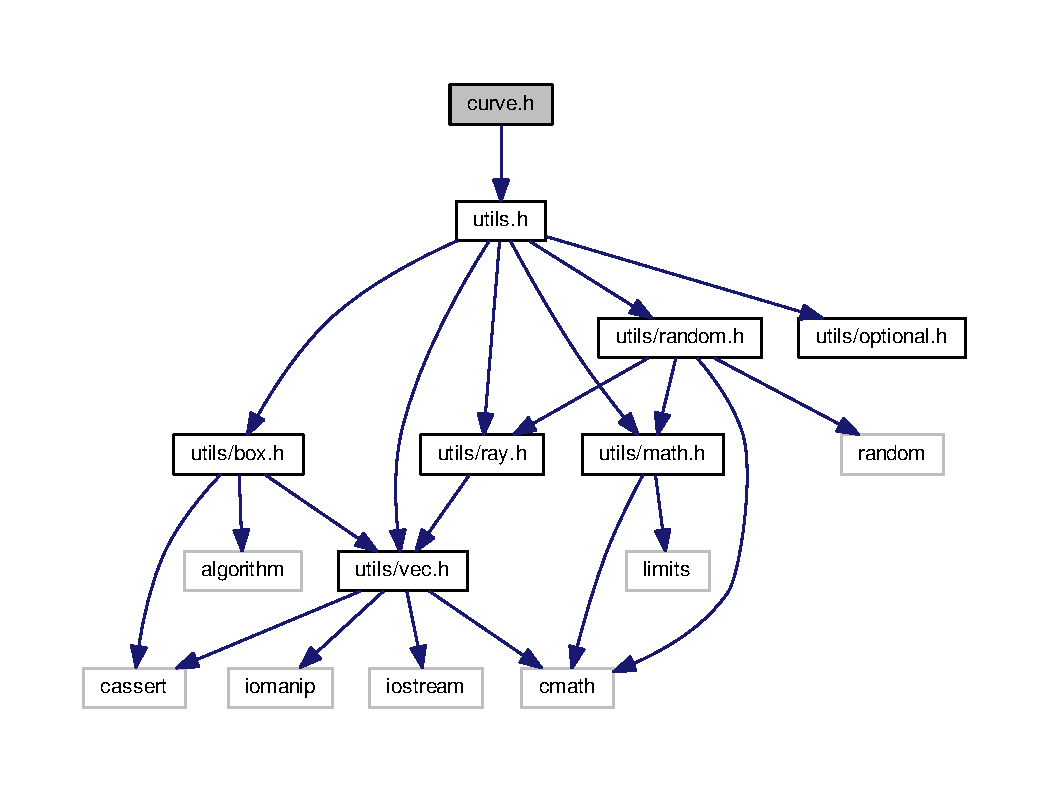
\includegraphics[width=350pt]{curve_8h__incl}
\end{center}
\end{figure}
This graph shows which files directly or indirectly include this file\+:
\nopagebreak
\begin{figure}[H]
\begin{center}
\leavevmode
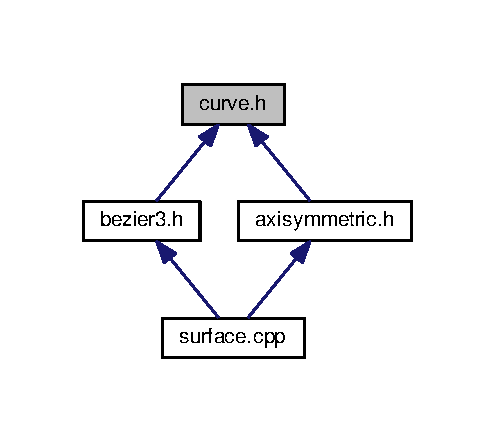
\includegraphics[width=238pt]{curve_8h__dep__incl}
\end{center}
\end{figure}
\subsection*{Classes}
\begin{DoxyCompactItemize}
\item 
class \hyperlink{classCurve}{Curve}
\begin{DoxyCompactList}\small\item\em \hyperlink{classCurve}{Curve} base class \hyperlink{classCurve}{Curve} with parameter t in \mbox{[}0,1\mbox{]}. \end{DoxyCompactList}\end{DoxyCompactItemize}

\hypertarget{debug_8cpp}{}\section{debug.\+cpp File Reference}
\label{debug_8cpp}\index{debug.\+cpp@{debug.\+cpp}}
{\ttfamily \#include $<$fstream$>$}\\*
{\ttfamily \#include \char`\"{}mesh.\+h\char`\"{}}\\*
{\ttfamily \#include \char`\"{}const.\+h\char`\"{}}\\*
{\ttfamily \#include \char`\"{}surface.\+h\char`\"{}}\\*
Include dependency graph for debug.\+cpp\+:\nopagebreak
\begin{figure}[H]
\begin{center}
\leavevmode
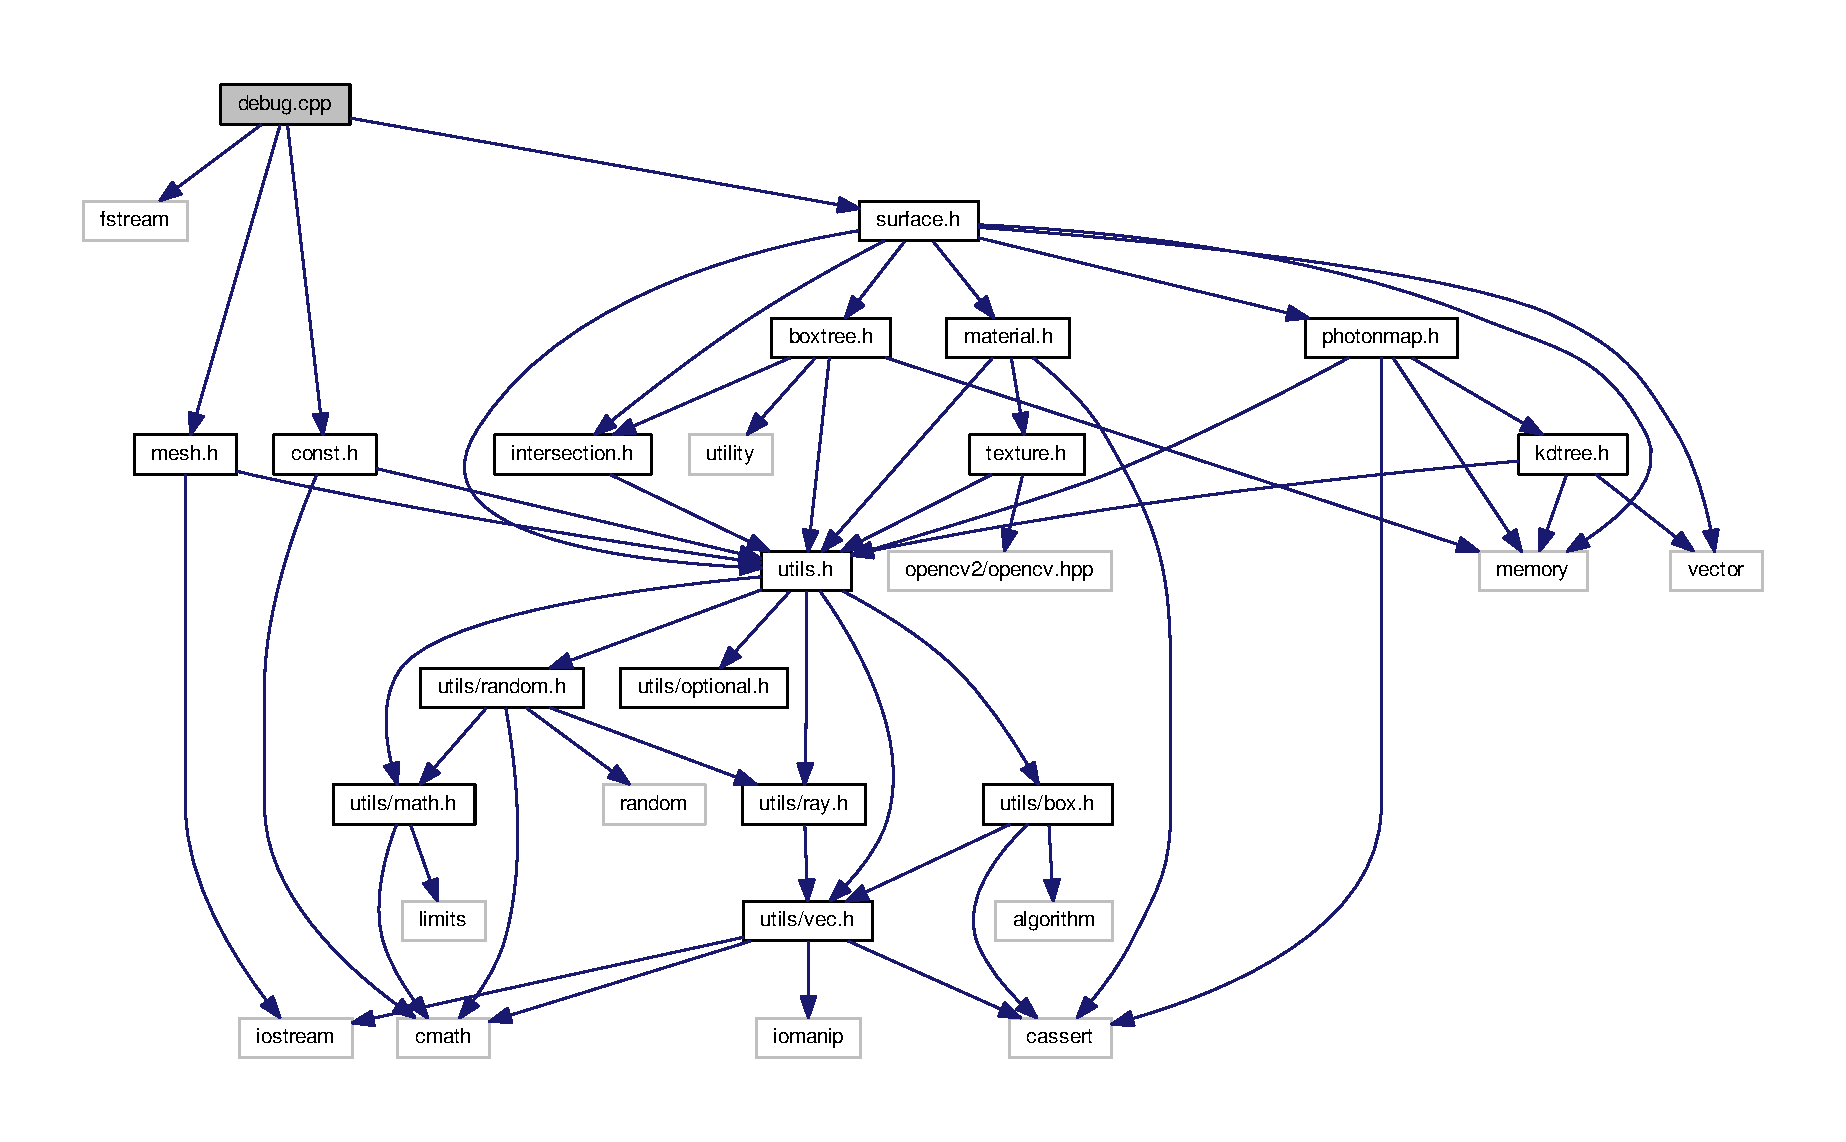
\includegraphics[width=350pt]{debug_8cpp__incl}
\end{center}
\end{figure}
\subsection*{Functions}
\begin{DoxyCompactItemize}
\item 
int \hyperlink{debug_8cpp_ae66f6b31b5ad750f1fe042a706a4e3d4}{main} ()
\begin{DoxyCompactList}\small\item\em Test intersection manually. \end{DoxyCompactList}\end{DoxyCompactItemize}


\subsection{Function Documentation}
\index{debug.\+cpp@{debug.\+cpp}!main@{main}}
\index{main@{main}!debug.\+cpp@{debug.\+cpp}}
\subsubsection[{\texorpdfstring{main()}{main()}}]{\setlength{\rightskip}{0pt plus 5cm}int main (
\begin{DoxyParamCaption}
{}
\end{DoxyParamCaption}
)}\hypertarget{debug_8cpp_ae66f6b31b5ad750f1fe042a706a4e3d4}{}\label{debug_8cpp_ae66f6b31b5ad750f1fe042a706a4e3d4}


Test intersection manually. 


\hypertarget{genmesh_8cpp}{}\section{genmesh.\+cpp File Reference}
\label{genmesh_8cpp}\index{genmesh.\+cpp@{genmesh.\+cpp}}
{\ttfamily \#include $<$fstream$>$}\\*
{\ttfamily \#include \char`\"{}mesh.\+h\char`\"{}}\\*
{\ttfamily \#include \char`\"{}const.\+h\char`\"{}}\\*
Include dependency graph for genmesh.\+cpp\+:\nopagebreak
\begin{figure}[H]
\begin{center}
\leavevmode
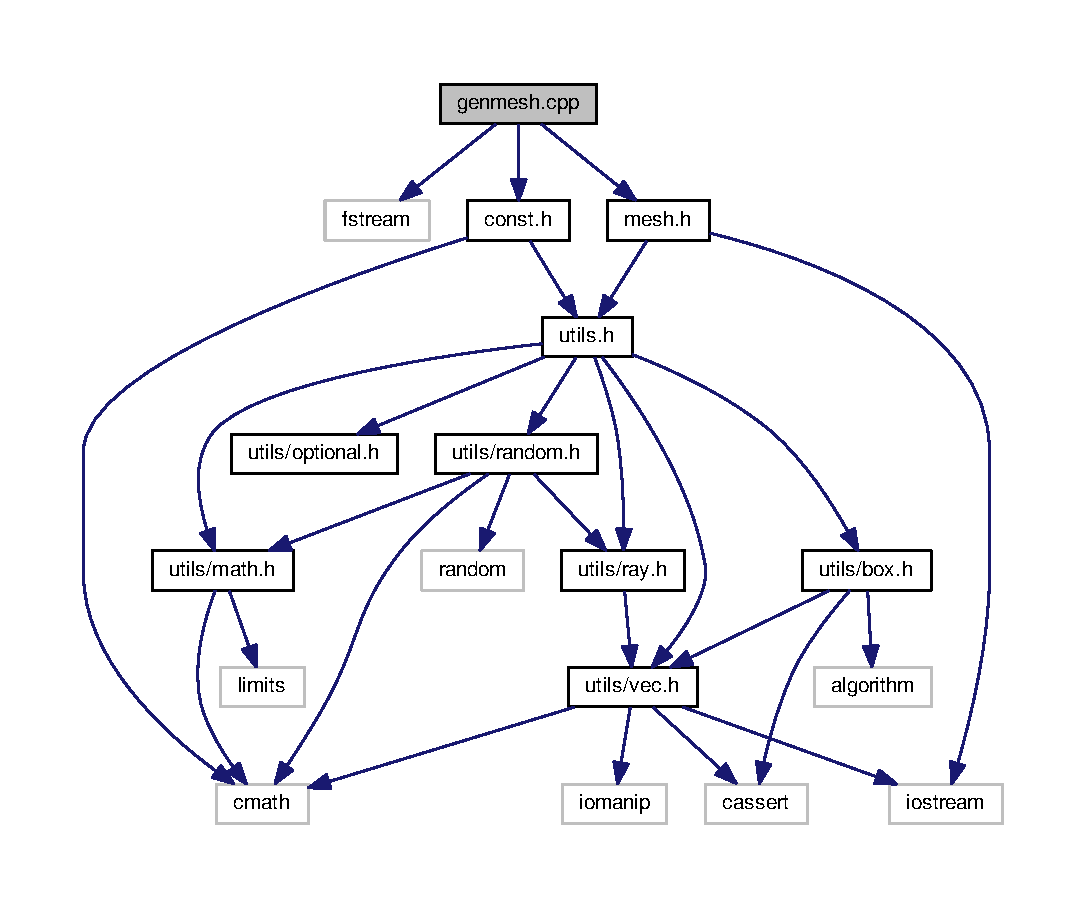
\includegraphics[width=350pt]{genmesh_8cpp__incl}
\end{center}
\end{figure}
\subsection*{Functions}
\begin{DoxyCompactItemize}
\item 
int \hyperlink{genmesh_8cpp_ae66f6b31b5ad750f1fe042a706a4e3d4}{main} ()
\begin{DoxyCompactList}\small\item\em Program used to generate meshes. \end{DoxyCompactList}\end{DoxyCompactItemize}


\subsection{Function Documentation}
\index{genmesh.\+cpp@{genmesh.\+cpp}!main@{main}}
\index{main@{main}!genmesh.\+cpp@{genmesh.\+cpp}}
\subsubsection[{\texorpdfstring{main()}{main()}}]{\setlength{\rightskip}{0pt plus 5cm}int main (
\begin{DoxyParamCaption}
{}
\end{DoxyParamCaption}
)}\hypertarget{genmesh_8cpp_ae66f6b31b5ad750f1fe042a706a4e3d4}{}\label{genmesh_8cpp_ae66f6b31b5ad750f1fe042a706a4e3d4}


Program used to generate meshes. 


\hypertarget{intersection_8cpp}{}\section{intersection.\+cpp File Reference}
\label{intersection_8cpp}\index{intersection.\+cpp@{intersection.\+cpp}}
{\ttfamily \#include $<$cassert$>$}\\*
{\ttfamily \#include \char`\"{}const.\+h\char`\"{}}\\*
{\ttfamily \#include \char`\"{}surface.\+h\char`\"{}}\\*
{\ttfamily \#include \char`\"{}intersection.\+h\char`\"{}}\\*
Include dependency graph for intersection.\+cpp\+:\nopagebreak
\begin{figure}[H]
\begin{center}
\leavevmode
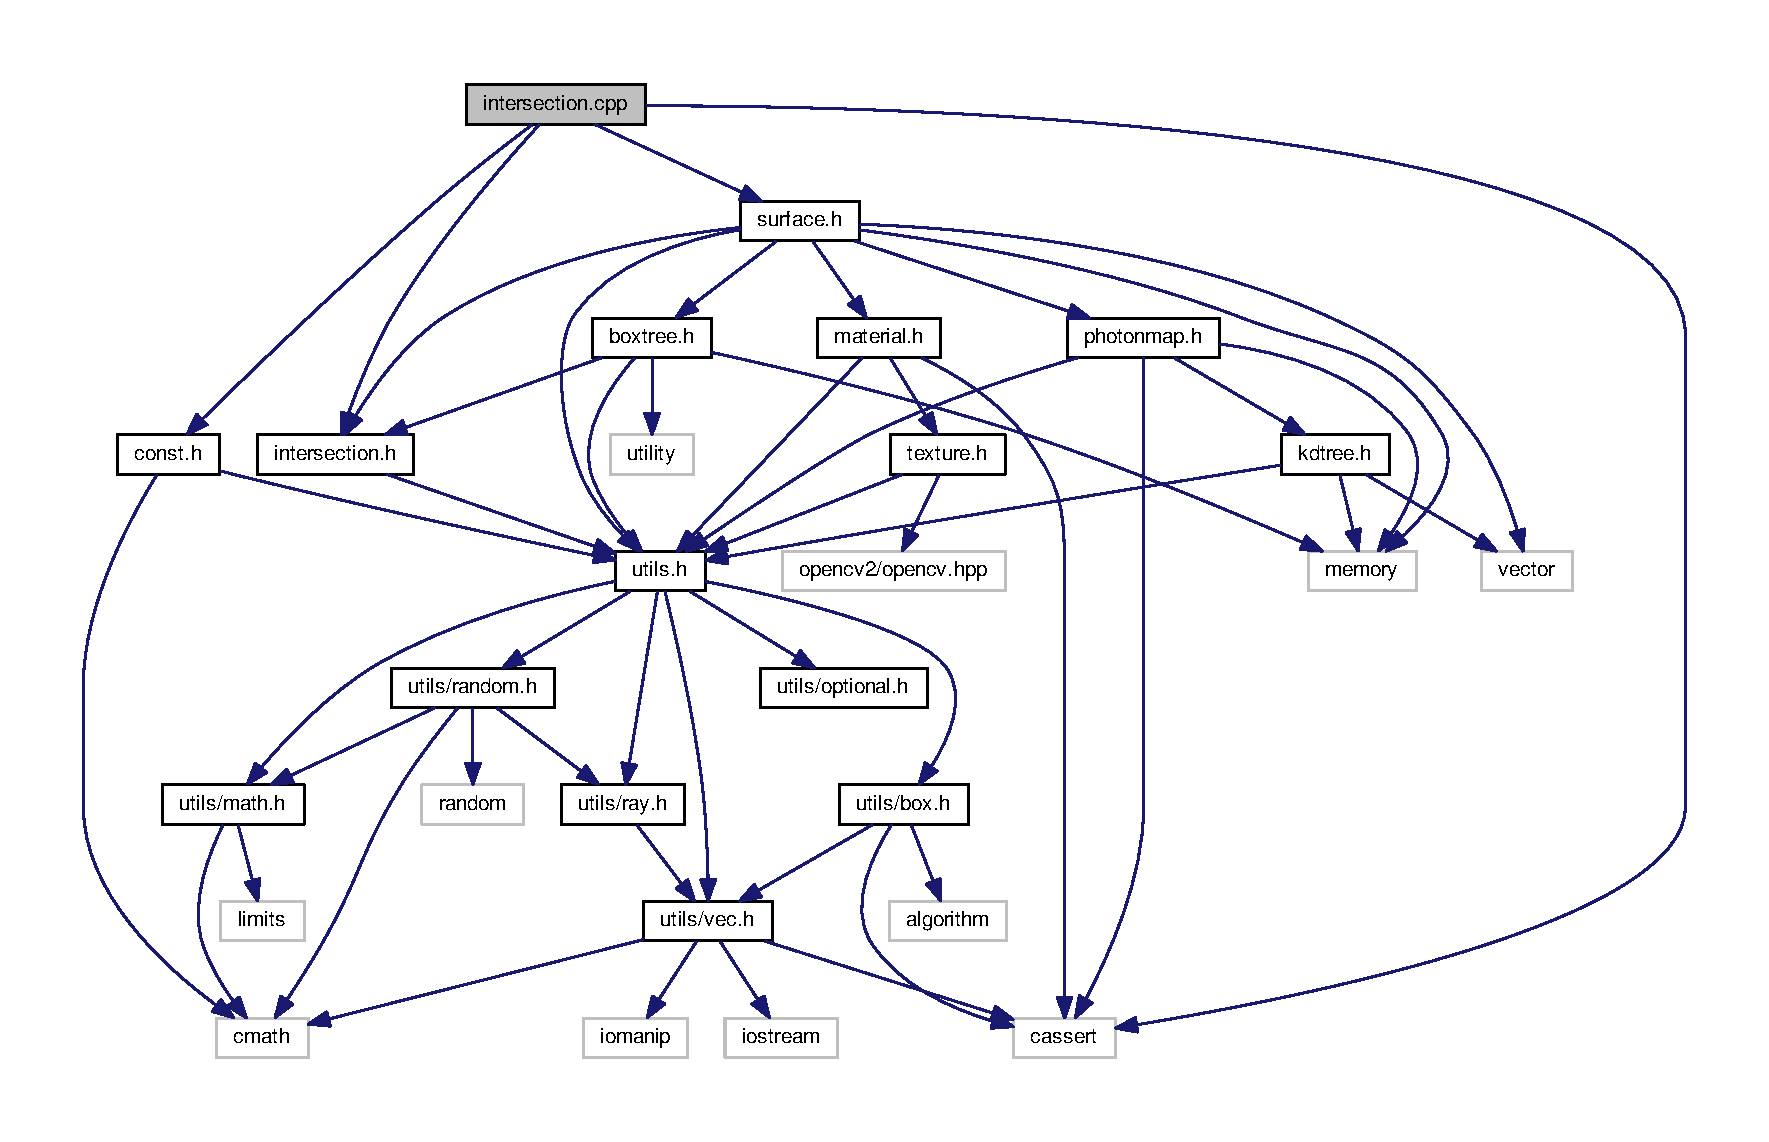
\includegraphics[width=350pt]{intersection_8cpp__incl}
\end{center}
\end{figure}
\subsection*{Functions}
\begin{DoxyCompactItemize}
\item 
\hyperlink{classOptional}{Optional}$<$ \hyperlink{intersection_8h_a880ab27cdd7ea5eab91289bba0bacadb}{Inter\+Type} $>$ \hyperlink{intersection_8cpp_a8d26d293d4190e1ae37cd92106d195de}{intersec\+YZ} (float x, const \hyperlink{structBox2}{Box2} \&box, const \hyperlink{structRay}{Ray} \&ray)
\begin{DoxyCompactList}\small\item\em These functinos find intersection between yz/xz/xy-\/plane and ray Asserting the ray intersecting with the extended infinte plane. \end{DoxyCompactList}\item 
\hyperlink{classOptional}{Optional}$<$ \hyperlink{intersection_8h_a880ab27cdd7ea5eab91289bba0bacadb}{Inter\+Type} $>$ \hyperlink{intersection_8cpp_ac2aaa5d853c940674478ca872272b443}{intersec\+XZ} (float y, const \hyperlink{structBox2}{Box2} \&box, const \hyperlink{structRay}{Ray} \&ray)
\item 
\hyperlink{classOptional}{Optional}$<$ \hyperlink{intersection_8h_a880ab27cdd7ea5eab91289bba0bacadb}{Inter\+Type} $>$ \hyperlink{intersection_8cpp_a92bc7a78315904bcef807c694583143b}{intersec\+XY} (float z, const \hyperlink{structBox2}{Box2} \&box, const \hyperlink{structRay}{Ray} \&ray)
\item 
\hyperlink{classOptional}{Optional}$<$ \hyperlink{intersection_8h_a880ab27cdd7ea5eab91289bba0bacadb}{Inter\+Type} $>$ \hyperlink{intersection_8cpp_afcbfaca43609cb5fdc84fde37a56857a}{intersec} (const \hyperlink{structBox3}{Box3} \&box, const \hyperlink{structRay}{Ray} \&ray)
\begin{DoxyCompactList}\small\item\em Find intersection between box and ray. \end{DoxyCompactList}\item 
\hyperlink{classOptional}{Optional}$<$ \hyperlink{structSurfInterType}{Surf\+Inter\+Type} $>$ \hyperlink{intersection_8cpp_ac780126b09d234c205b14017ed48cc0e}{intersec} (float t, float u, float v, const \hyperlink{vec_8h_ae4fcaa7c0a3935930ed1be5f70b90373}{Vec3} \&p0, const \hyperlink{classSurface}{Surface} \&surf, const \hyperlink{structRay}{Ray} \&ray)
\begin{DoxyCompactList}\small\item\em Find intersection with a surface based on box intersection. \end{DoxyCompactList}\end{DoxyCompactItemize}


\subsection{Function Documentation}
\index{intersection.\+cpp@{intersection.\+cpp}!intersec@{intersec}}
\index{intersec@{intersec}!intersection.\+cpp@{intersection.\+cpp}}
\subsubsection[{\texorpdfstring{intersec(const Box3 \&box, const Ray \&ray)}{intersec(const Box3 &box, const Ray &ray)}}]{\setlength{\rightskip}{0pt plus 5cm}{\bf Optional}$<${\bf Inter\+Type}$>$ intersec (
\begin{DoxyParamCaption}
\item[{const {\bf Box3} \&}]{box, }
\item[{const {\bf Ray} \&}]{ray}
\end{DoxyParamCaption}
)}\hypertarget{intersection_8cpp_afcbfaca43609cb5fdc84fde37a56857a}{}\label{intersection_8cpp_afcbfaca43609cb5fdc84fde37a56857a}


Find intersection between box and ray. 

\begin{DoxyReturn}{Returns}
\+: (Intersection point, \hyperlink{structRay}{Ray} parameter) 
\end{DoxyReturn}
\index{intersection.\+cpp@{intersection.\+cpp}!intersec@{intersec}}
\index{intersec@{intersec}!intersection.\+cpp@{intersection.\+cpp}}
\subsubsection[{\texorpdfstring{intersec(float t, float u, float v, const Vec3 \&p0, const Surface \&surf, const Ray \&ray)}{intersec(float t, float u, float v, const Vec3 &p0, const Surface &surf, const Ray &ray)}}]{\setlength{\rightskip}{0pt plus 5cm}{\bf Optional}$<${\bf Surf\+Inter\+Type}$>$ intersec (
\begin{DoxyParamCaption}
\item[{float}]{t, }
\item[{float}]{u, }
\item[{float}]{v, }
\item[{const {\bf Vec3} \&}]{p0, }
\item[{const {\bf Surface} \&}]{surf, }
\item[{const {\bf Ray} \&}]{ray}
\end{DoxyParamCaption}
)}\hypertarget{intersection_8cpp_ac780126b09d234c205b14017ed48cc0e}{}\label{intersection_8cpp_ac780126b09d234c205b14017ed48cc0e}


Find intersection with a surface based on box intersection. 


\begin{DoxyParams}{Parameters}
{\em t,u,v} & \+: Initial values \\
\hline
{\em p0} & \+: Initial intersection \\
\hline
\end{DoxyParams}
\index{intersection.\+cpp@{intersection.\+cpp}!intersec\+XY@{intersec\+XY}}
\index{intersec\+XY@{intersec\+XY}!intersection.\+cpp@{intersection.\+cpp}}
\subsubsection[{\texorpdfstring{intersec\+X\+Y(float z, const Box2 \&box, const Ray \&ray)}{intersecXY(float z, const Box2 &box, const Ray &ray)}}]{\setlength{\rightskip}{0pt plus 5cm}{\bf Optional}$<${\bf Inter\+Type}$>$ intersec\+XY (
\begin{DoxyParamCaption}
\item[{float}]{z, }
\item[{const {\bf Box2} \&}]{box, }
\item[{const {\bf Ray} \&}]{ray}
\end{DoxyParamCaption}
)}\hypertarget{intersection_8cpp_a92bc7a78315904bcef807c694583143b}{}\label{intersection_8cpp_a92bc7a78315904bcef807c694583143b}
\index{intersection.\+cpp@{intersection.\+cpp}!intersec\+XZ@{intersec\+XZ}}
\index{intersec\+XZ@{intersec\+XZ}!intersection.\+cpp@{intersection.\+cpp}}
\subsubsection[{\texorpdfstring{intersec\+X\+Z(float y, const Box2 \&box, const Ray \&ray)}{intersecXZ(float y, const Box2 &box, const Ray &ray)}}]{\setlength{\rightskip}{0pt plus 5cm}{\bf Optional}$<${\bf Inter\+Type}$>$ intersec\+XZ (
\begin{DoxyParamCaption}
\item[{float}]{y, }
\item[{const {\bf Box2} \&}]{box, }
\item[{const {\bf Ray} \&}]{ray}
\end{DoxyParamCaption}
)}\hypertarget{intersection_8cpp_ac2aaa5d853c940674478ca872272b443}{}\label{intersection_8cpp_ac2aaa5d853c940674478ca872272b443}
\index{intersection.\+cpp@{intersection.\+cpp}!intersec\+YZ@{intersec\+YZ}}
\index{intersec\+YZ@{intersec\+YZ}!intersection.\+cpp@{intersection.\+cpp}}
\subsubsection[{\texorpdfstring{intersec\+Y\+Z(float x, const Box2 \&box, const Ray \&ray)}{intersecYZ(float x, const Box2 &box, const Ray &ray)}}]{\setlength{\rightskip}{0pt plus 5cm}{\bf Optional}$<${\bf Inter\+Type}$>$ intersec\+YZ (
\begin{DoxyParamCaption}
\item[{float}]{x, }
\item[{const {\bf Box2} \&}]{box, }
\item[{const {\bf Ray} \&}]{ray}
\end{DoxyParamCaption}
)}\hypertarget{intersection_8cpp_a8d26d293d4190e1ae37cd92106d195de}{}\label{intersection_8cpp_a8d26d293d4190e1ae37cd92106d195de}


These functinos find intersection between yz/xz/xy-\/plane and ray Asserting the ray intersecting with the extended infinte plane. 


\begin{DoxyParams}{Parameters}
{\em x,y,z} & \+: Plane position \\
\hline
{\em box} & \+: Plane size \\
\hline
\end{DoxyParams}
\begin{DoxyReturn}{Returns}
\+: (Intersection point, \hyperlink{structRay}{Ray} parameter) 
\end{DoxyReturn}

\hypertarget{intersection_8h}{}\section{intersection.\+h File Reference}
\label{intersection_8h}\index{intersection.\+h@{intersection.\+h}}
{\ttfamily \#include \char`\"{}utils.\+h\char`\"{}}\\*
Include dependency graph for intersection.\+h\+:\nopagebreak
\begin{figure}[H]
\begin{center}
\leavevmode
\includegraphics[width=350pt]{intersection_8h__incl}
\end{center}
\end{figure}
This graph shows which files directly or indirectly include this file\+:\nopagebreak
\begin{figure}[H]
\begin{center}
\leavevmode
\includegraphics[width=350pt]{intersection_8h__dep__incl}
\end{center}
\end{figure}
\subsection*{Classes}
\begin{DoxyCompactItemize}
\item 
struct \hyperlink{structSurfInterType}{Surf\+Inter\+Type}
\end{DoxyCompactItemize}
\subsection*{Typedefs}
\begin{DoxyCompactItemize}
\item 
typedef std\+::pair$<$ \hyperlink{vec_8h_ae4fcaa7c0a3935930ed1be5f70b90373}{Vec3}, float $>$ \hyperlink{intersection_8h_a880ab27cdd7ea5eab91289bba0bacadb}{Inter\+Type}
\end{DoxyCompactItemize}
\subsection*{Functions}
\begin{DoxyCompactItemize}
\item 
\hyperlink{classOptional}{Optional}$<$ \hyperlink{intersection_8h_a880ab27cdd7ea5eab91289bba0bacadb}{Inter\+Type} $>$ \hyperlink{intersection_8h_a8d26d293d4190e1ae37cd92106d195de}{intersec\+YZ} (float x, const \hyperlink{structBox2}{Box2} \&box, const \hyperlink{structRay}{Ray} \&ray)
\begin{DoxyCompactList}\small\item\em These functinos find intersection between yz/xz/xy-\/plane and ray Asserting the ray intersecting with the extended infinte plane. \end{DoxyCompactList}\item 
\hyperlink{classOptional}{Optional}$<$ \hyperlink{intersection_8h_a880ab27cdd7ea5eab91289bba0bacadb}{Inter\+Type} $>$ \hyperlink{intersection_8h_ac2aaa5d853c940674478ca872272b443}{intersec\+XZ} (float y, const \hyperlink{structBox2}{Box2} \&box, const \hyperlink{structRay}{Ray} \&ray)
\item 
\hyperlink{classOptional}{Optional}$<$ \hyperlink{intersection_8h_a880ab27cdd7ea5eab91289bba0bacadb}{Inter\+Type} $>$ \hyperlink{intersection_8h_a92bc7a78315904bcef807c694583143b}{intersec\+XY} (float z, const \hyperlink{structBox2}{Box2} \&box, const \hyperlink{structRay}{Ray} \&ray)
\item 
\hyperlink{classOptional}{Optional}$<$ \hyperlink{intersection_8h_a880ab27cdd7ea5eab91289bba0bacadb}{Inter\+Type} $>$ \hyperlink{intersection_8h_afcbfaca43609cb5fdc84fde37a56857a}{intersec} (const \hyperlink{structBox3}{Box3} \&box, const \hyperlink{structRay}{Ray} \&ray)
\begin{DoxyCompactList}\small\item\em Find intersection between box and ray. \end{DoxyCompactList}\item 
\hyperlink{classOptional}{Optional}$<$ \hyperlink{structSurfInterType}{Surf\+Inter\+Type} $>$ \hyperlink{intersection_8h_ac780126b09d234c205b14017ed48cc0e}{intersec} (float t, float u, float v, const \hyperlink{vec_8h_ae4fcaa7c0a3935930ed1be5f70b90373}{Vec3} \&p0, const \hyperlink{classSurface}{Surface} \&surf, const \hyperlink{structRay}{Ray} \&ray)
\begin{DoxyCompactList}\small\item\em Find intersection with a surface based on box intersection. \end{DoxyCompactList}\end{DoxyCompactItemize}


\subsection{Typedef Documentation}
\index{intersection.\+h@{intersection.\+h}!Inter\+Type@{Inter\+Type}}
\index{Inter\+Type@{Inter\+Type}!intersection.\+h@{intersection.\+h}}
\subsubsection[{\texorpdfstring{Inter\+Type}{InterType}}]{\setlength{\rightskip}{0pt plus 5cm}typedef std\+::pair$<${\bf Vec3}, float$>$ {\bf Inter\+Type}}\hypertarget{intersection_8h_a880ab27cdd7ea5eab91289bba0bacadb}{}\label{intersection_8h_a880ab27cdd7ea5eab91289bba0bacadb}


\subsection{Function Documentation}
\index{intersection.\+h@{intersection.\+h}!intersec@{intersec}}
\index{intersec@{intersec}!intersection.\+h@{intersection.\+h}}
\subsubsection[{\texorpdfstring{intersec(const Box3 \&box, const Ray \&ray)}{intersec(const Box3 &box, const Ray &ray)}}]{\setlength{\rightskip}{0pt plus 5cm}{\bf Optional}$<${\bf Inter\+Type}$>$ intersec (
\begin{DoxyParamCaption}
\item[{const {\bf Box3} \&}]{box, }
\item[{const {\bf Ray} \&}]{ray}
\end{DoxyParamCaption}
)}\hypertarget{intersection_8h_afcbfaca43609cb5fdc84fde37a56857a}{}\label{intersection_8h_afcbfaca43609cb5fdc84fde37a56857a}


Find intersection between box and ray. 

\begin{DoxyReturn}{Returns}
\+: (Intersection point, \hyperlink{structRay}{Ray} parameter) 
\end{DoxyReturn}
\index{intersection.\+h@{intersection.\+h}!intersec@{intersec}}
\index{intersec@{intersec}!intersection.\+h@{intersection.\+h}}
\subsubsection[{\texorpdfstring{intersec(float t, float u, float v, const Vec3 \&p0, const Surface \&surf, const Ray \&ray)}{intersec(float t, float u, float v, const Vec3 &p0, const Surface &surf, const Ray &ray)}}]{\setlength{\rightskip}{0pt plus 5cm}{\bf Optional}$<${\bf Surf\+Inter\+Type}$>$ intersec (
\begin{DoxyParamCaption}
\item[{float}]{t, }
\item[{float}]{u, }
\item[{float}]{v, }
\item[{const {\bf Vec3} \&}]{p0, }
\item[{const {\bf Surface} \&}]{surf, }
\item[{const {\bf Ray} \&}]{ray}
\end{DoxyParamCaption}
)}\hypertarget{intersection_8h_ac780126b09d234c205b14017ed48cc0e}{}\label{intersection_8h_ac780126b09d234c205b14017ed48cc0e}


Find intersection with a surface based on box intersection. 


\begin{DoxyParams}{Parameters}
{\em t,u,v} & \+: Initial values \\
\hline
{\em p0} & \+: Initial intersection \\
\hline
\end{DoxyParams}
\index{intersection.\+h@{intersection.\+h}!intersec\+XY@{intersec\+XY}}
\index{intersec\+XY@{intersec\+XY}!intersection.\+h@{intersection.\+h}}
\subsubsection[{\texorpdfstring{intersec\+X\+Y(float z, const Box2 \&box, const Ray \&ray)}{intersecXY(float z, const Box2 &box, const Ray &ray)}}]{\setlength{\rightskip}{0pt plus 5cm}{\bf Optional}$<${\bf Inter\+Type}$>$ intersec\+XY (
\begin{DoxyParamCaption}
\item[{float}]{z, }
\item[{const {\bf Box2} \&}]{box, }
\item[{const {\bf Ray} \&}]{ray}
\end{DoxyParamCaption}
)}\hypertarget{intersection_8h_a92bc7a78315904bcef807c694583143b}{}\label{intersection_8h_a92bc7a78315904bcef807c694583143b}
\index{intersection.\+h@{intersection.\+h}!intersec\+XZ@{intersec\+XZ}}
\index{intersec\+XZ@{intersec\+XZ}!intersection.\+h@{intersection.\+h}}
\subsubsection[{\texorpdfstring{intersec\+X\+Z(float y, const Box2 \&box, const Ray \&ray)}{intersecXZ(float y, const Box2 &box, const Ray &ray)}}]{\setlength{\rightskip}{0pt plus 5cm}{\bf Optional}$<${\bf Inter\+Type}$>$ intersec\+XZ (
\begin{DoxyParamCaption}
\item[{float}]{y, }
\item[{const {\bf Box2} \&}]{box, }
\item[{const {\bf Ray} \&}]{ray}
\end{DoxyParamCaption}
)}\hypertarget{intersection_8h_ac2aaa5d853c940674478ca872272b443}{}\label{intersection_8h_ac2aaa5d853c940674478ca872272b443}
\index{intersection.\+h@{intersection.\+h}!intersec\+YZ@{intersec\+YZ}}
\index{intersec\+YZ@{intersec\+YZ}!intersection.\+h@{intersection.\+h}}
\subsubsection[{\texorpdfstring{intersec\+Y\+Z(float x, const Box2 \&box, const Ray \&ray)}{intersecYZ(float x, const Box2 &box, const Ray &ray)}}]{\setlength{\rightskip}{0pt plus 5cm}{\bf Optional}$<${\bf Inter\+Type}$>$ intersec\+YZ (
\begin{DoxyParamCaption}
\item[{float}]{x, }
\item[{const {\bf Box2} \&}]{box, }
\item[{const {\bf Ray} \&}]{ray}
\end{DoxyParamCaption}
)}\hypertarget{intersection_8h_a8d26d293d4190e1ae37cd92106d195de}{}\label{intersection_8h_a8d26d293d4190e1ae37cd92106d195de}


These functinos find intersection between yz/xz/xy-\/plane and ray Asserting the ray intersecting with the extended infinte plane. 


\begin{DoxyParams}{Parameters}
{\em x,y,z} & \+: Plane position \\
\hline
{\em box} & \+: Plane size \\
\hline
\end{DoxyParams}
\begin{DoxyReturn}{Returns}
\+: (Intersection point, \hyperlink{structRay}{Ray} parameter) 
\end{DoxyReturn}

\hypertarget{kdtree_8cpp}{}\section{kdtree.\+cpp File Reference}
\label{kdtree_8cpp}\index{kdtree.\+cpp@{kdtree.\+cpp}}
{\ttfamily \#include $<$cassert$>$}\\*
{\ttfamily \#include $<$algorithm$>$}\\*
{\ttfamily \#include \char`\"{}kdtree.\+h\char`\"{}}\\*
Include dependency graph for kdtree.\+cpp\+:
\nopagebreak
\begin{figure}[H]
\begin{center}
\leavevmode
\includegraphics[width=350pt]{kdtree_8cpp__incl}
\end{center}
\end{figure}

\hypertarget{kdtree_8h}{}\section{kdtree.\+h File Reference}
\label{kdtree_8h}\index{kdtree.\+h@{kdtree.\+h}}
{\ttfamily \#include $<$memory$>$}\\*
{\ttfamily \#include $<$vector$>$}\\*
{\ttfamily \#include \char`\"{}utils.\+h\char`\"{}}\\*
Include dependency graph for kdtree.\+h\+:\nopagebreak
\begin{figure}[H]
\begin{center}
\leavevmode
\includegraphics[width=350pt]{kdtree_8h__incl}
\end{center}
\end{figure}
This graph shows which files directly or indirectly include this file\+:\nopagebreak
\begin{figure}[H]
\begin{center}
\leavevmode
\includegraphics[width=350pt]{kdtree_8h__dep__incl}
\end{center}
\end{figure}
\subsection*{Classes}
\begin{DoxyCompactItemize}
\item 
class \hyperlink{classKDTree}{K\+D\+Tree}
\item 
struct \hyperlink{structKDTree_1_1Node}{K\+D\+Tree\+::\+Node}
\end{DoxyCompactItemize}

\hypertarget{lightsource_8h}{}\section{lightsource.\+h File Reference}
\label{lightsource_8h}\index{lightsource.\+h@{lightsource.\+h}}
{\ttfamily \#include $<$cmath$>$}\\*
{\ttfamily \#include $<$cassert$>$}\\*
{\ttfamily \#include \char`\"{}../const.\+h\char`\"{}}\\*
{\ttfamily \#include \char`\"{}../utils.\+h\char`\"{}}\\*
{\ttfamily \#include \char`\"{}../surface.\+h\char`\"{}}\\*
{\ttfamily \#include \char`\"{}../intersection.\+h\char`\"{}}\\*
Include dependency graph for lightsource.\+h\+:
\nopagebreak
\begin{figure}[H]
\begin{center}
\leavevmode
\includegraphics[width=350pt]{lightsource_8h__incl}
\end{center}
\end{figure}
This graph shows which files directly or indirectly include this file\+:
\nopagebreak
\begin{figure}[H]
\begin{center}
\leavevmode
\includegraphics[width=222pt]{lightsource_8h__dep__incl}
\end{center}
\end{figure}
\subsection*{Classes}
\begin{DoxyCompactItemize}
\item 
class \hyperlink{classLightSource}{Light\+Source}
\begin{DoxyCompactList}\small\item\em Light source as a ball Cannot be used as a normal object. \end{DoxyCompactList}\end{DoxyCompactItemize}

\hypertarget{main_8cpp}{}\section{main.\+cpp File Reference}
\label{main_8cpp}\index{main.\+cpp@{main.\+cpp}}
{\ttfamily \#include $<$cstring$>$}\\*
{\ttfamily \#include $<$vector$>$}\\*
{\ttfamily \#include $<$fstream$>$}\\*
{\ttfamily \#include $<$random$>$}\\*
{\ttfamily \#include $<$iostream$>$}\\*
{\ttfamily \#include $<$opencv2/opencv.\+hpp$>$}\\*
{\ttfamily \#include \char`\"{}trace.\+h\char`\"{}}\\*
{\ttfamily \#include \char`\"{}utils.\+h\char`\"{}}\\*
{\ttfamily \#include \char`\"{}const.\+h\char`\"{}}\\*
{\ttfamily \#include \char`\"{}surface.\+h\char`\"{}}\\*
{\ttfamily \#include \char`\"{}photonmap.\+h\char`\"{}}\\*
{\ttfamily \#include \char`\"{}surface/lightsource.\+h\char`\"{}}\\*
Include dependency graph for main.\+cpp\+:
\nopagebreak
\begin{figure}[H]
\begin{center}
\leavevmode
\includegraphics[width=350pt]{main_8cpp__incl}
\end{center}
\end{figure}
\subsection*{Functions}
\begin{DoxyCompactItemize}
\item 
void \hyperlink{main_8cpp_ab2df3b0fe26c019e681f886165abba6b}{emit} (const std\+::vector$<$ std\+::unique\+\_\+ptr$<$ \hyperlink{classSurface}{Surface} $>$ $>$ \&surfaces)
\item 
void \hyperlink{main_8cpp_adcfddd2cd76dbfe2599dd1b27585a6c4}{build} (const std\+::vector$<$ std\+::unique\+\_\+ptr$<$ \hyperlink{classSurface}{Surface} $>$ $>$ \&surfaces)
\item 
void \hyperlink{main_8cpp_a0a33279211b722d1ee2e112187ceedaa}{collect} (const std\+::vector$<$ std\+::unique\+\_\+ptr$<$ \hyperlink{classSurface}{Surface} $>$ $>$ \&surfaces, cv\+::\+Mat3b \&canvas)
\item 
int \hyperlink{main_8cpp_ae66f6b31b5ad750f1fe042a706a4e3d4}{main} ()
\end{DoxyCompactItemize}


\subsection{Function Documentation}
\index{main.\+cpp@{main.\+cpp}!build@{build}}
\index{build@{build}!main.\+cpp@{main.\+cpp}}
\subsubsection[{\texorpdfstring{build(const std\+::vector$<$ std\+::unique\+\_\+ptr$<$ Surface $>$ $>$ \&surfaces)}{build(const std::vector< std::unique_ptr< Surface > > &surfaces)}}]{\setlength{\rightskip}{0pt plus 5cm}void build (
\begin{DoxyParamCaption}
\item[{const std\+::vector$<$ std\+::unique\+\_\+ptr$<$ {\bf Surface} $>$ $>$ \&}]{surfaces}
\end{DoxyParamCaption}
)}\hypertarget{main_8cpp_adcfddd2cd76dbfe2599dd1b27585a6c4}{}\label{main_8cpp_adcfddd2cd76dbfe2599dd1b27585a6c4}
\index{main.\+cpp@{main.\+cpp}!collect@{collect}}
\index{collect@{collect}!main.\+cpp@{main.\+cpp}}
\subsubsection[{\texorpdfstring{collect(const std\+::vector$<$ std\+::unique\+\_\+ptr$<$ Surface $>$ $>$ \&surfaces, cv\+::\+Mat3b \&canvas)}{collect(const std::vector< std::unique_ptr< Surface > > &surfaces, cv::Mat3b &canvas)}}]{\setlength{\rightskip}{0pt plus 5cm}void collect (
\begin{DoxyParamCaption}
\item[{const std\+::vector$<$ std\+::unique\+\_\+ptr$<$ {\bf Surface} $>$ $>$ \&}]{surfaces, }
\item[{cv\+::\+Mat3b \&}]{canvas}
\end{DoxyParamCaption}
)}\hypertarget{main_8cpp_a0a33279211b722d1ee2e112187ceedaa}{}\label{main_8cpp_a0a33279211b722d1ee2e112187ceedaa}
\index{main.\+cpp@{main.\+cpp}!emit@{emit}}
\index{emit@{emit}!main.\+cpp@{main.\+cpp}}
\subsubsection[{\texorpdfstring{emit(const std\+::vector$<$ std\+::unique\+\_\+ptr$<$ Surface $>$ $>$ \&surfaces)}{emit(const std::vector< std::unique_ptr< Surface > > &surfaces)}}]{\setlength{\rightskip}{0pt plus 5cm}void emit (
\begin{DoxyParamCaption}
\item[{const std\+::vector$<$ std\+::unique\+\_\+ptr$<$ {\bf Surface} $>$ $>$ \&}]{surfaces}
\end{DoxyParamCaption}
)}\hypertarget{main_8cpp_ab2df3b0fe26c019e681f886165abba6b}{}\label{main_8cpp_ab2df3b0fe26c019e681f886165abba6b}
Thread safe \index{main.\+cpp@{main.\+cpp}!main@{main}}
\index{main@{main}!main.\+cpp@{main.\+cpp}}
\subsubsection[{\texorpdfstring{main()}{main()}}]{\setlength{\rightskip}{0pt plus 5cm}int main (
\begin{DoxyParamCaption}
{}
\end{DoxyParamCaption}
)}\hypertarget{main_8cpp_ae66f6b31b5ad750f1fe042a706a4e3d4}{}\label{main_8cpp_ae66f6b31b5ad750f1fe042a706a4e3d4}

\hypertarget{material_8h}{}\section{material.\+h File Reference}
\label{material_8h}\index{material.\+h@{material.\+h}}
{\ttfamily \#include $<$cassert$>$}\\*
{\ttfamily \#include \char`\"{}utils.\+h\char`\"{}}\\*
{\ttfamily \#include \char`\"{}texture.\+h\char`\"{}}\\*
Include dependency graph for material.\+h\+:
\nopagebreak
\begin{figure}[H]
\begin{center}
\leavevmode
\includegraphics[width=350pt]{material_8h__incl}
\end{center}
\end{figure}
This graph shows which files directly or indirectly include this file\+:
\nopagebreak
\begin{figure}[H]
\begin{center}
\leavevmode
\includegraphics[width=350pt]{material_8h__dep__incl}
\end{center}
\end{figure}
\subsection*{Classes}
\begin{DoxyCompactItemize}
\item 
struct \hyperlink{structMaterial}{Material}
\end{DoxyCompactItemize}

\hypertarget{math_8h}{}\section{math.\+h File Reference}
\label{math_8h}\index{math.\+h@{math.\+h}}
{\ttfamily \#include $<$cmath$>$}\\*
{\ttfamily \#include $<$limits$>$}\\*
Include dependency graph for math.\+h\+:\nopagebreak
\begin{figure}[H]
\begin{center}
\leavevmode
\includegraphics[width=182pt]{math_8h__incl}
\end{center}
\end{figure}
This graph shows which files directly or indirectly include this file\+:\nopagebreak
\begin{figure}[H]
\begin{center}
\leavevmode
\includegraphics[width=350pt]{math_8h__dep__incl}
\end{center}
\end{figure}
\subsection*{Functions}
\begin{DoxyCompactItemize}
\item 
{\footnotesize template$<$class T $>$ }\\T \hyperlink{math_8h_a3de9ba6f9ac6ab92c5a2e86fded6f322}{sqr} (T x)
\end{DoxyCompactItemize}
\subsection*{Variables}
\begin{DoxyCompactItemize}
\item 
const float \hyperlink{math_8h_a8fc10aaaeb2ccece51baa85a4bcebb5f}{I\+NF} = std\+::numeric\+\_\+limits$<$float$>$\+::infinity()
\item 
const float \hyperlink{math_8h_aa08a577393243b86dfd2a97e61443673}{PI} = acosf(-\/1)
\end{DoxyCompactItemize}


\subsection{Function Documentation}
\index{math.\+h@{math.\+h}!sqr@{sqr}}
\index{sqr@{sqr}!math.\+h@{math.\+h}}
\subsubsection[{\texorpdfstring{sqr(\+T x)}{sqr(T x)}}]{\setlength{\rightskip}{0pt plus 5cm}template$<$class T $>$ T sqr (
\begin{DoxyParamCaption}
\item[{T}]{x}
\end{DoxyParamCaption}
)}\hypertarget{math_8h_a3de9ba6f9ac6ab92c5a2e86fded6f322}{}\label{math_8h_a3de9ba6f9ac6ab92c5a2e86fded6f322}


\subsection{Variable Documentation}
\index{math.\+h@{math.\+h}!I\+NF@{I\+NF}}
\index{I\+NF@{I\+NF}!math.\+h@{math.\+h}}
\subsubsection[{\texorpdfstring{I\+NF}{INF}}]{\setlength{\rightskip}{0pt plus 5cm}const float I\+NF = std\+::numeric\+\_\+limits$<$float$>$\+::infinity()}\hypertarget{math_8h_a8fc10aaaeb2ccece51baa85a4bcebb5f}{}\label{math_8h_a8fc10aaaeb2ccece51baa85a4bcebb5f}
\index{math.\+h@{math.\+h}!PI@{PI}}
\index{PI@{PI}!math.\+h@{math.\+h}}
\subsubsection[{\texorpdfstring{PI}{PI}}]{\setlength{\rightskip}{0pt plus 5cm}const float PI = acosf(-\/1)}\hypertarget{math_8h_aa08a577393243b86dfd2a97e61443673}{}\label{math_8h_aa08a577393243b86dfd2a97e61443673}

\hypertarget{mesh_8cpp}{}\section{mesh.\+cpp File Reference}
\label{mesh_8cpp}\index{mesh.\+cpp@{mesh.\+cpp}}
{\ttfamily \#include \char`\"{}mesh.\+h\char`\"{}}\\*
{\ttfamily \#include \char`\"{}const.\+h\char`\"{}}\\*
{\ttfamily \#include \char`\"{}surface.\+h\char`\"{}}\\*
Include dependency graph for mesh.\+cpp\+:\nopagebreak
\begin{figure}[H]
\begin{center}
\leavevmode
\includegraphics[width=350pt]{mesh_8cpp__incl}
\end{center}
\end{figure}

\hypertarget{mesh_8h}{}\section{mesh.\+h File Reference}
\label{mesh_8h}\index{mesh.\+h@{mesh.\+h}}
{\ttfamily \#include \char`\"{}utils.\+h\char`\"{}}\\*
{\ttfamily \#include $<$iostream$>$}\\*
Include dependency graph for mesh.\+h\+:
\nopagebreak
\begin{figure}[H]
\begin{center}
\leavevmode
\includegraphics[width=350pt]{mesh_8h__incl}
\end{center}
\end{figure}
This graph shows which files directly or indirectly include this file\+:
\nopagebreak
\begin{figure}[H]
\begin{center}
\leavevmode
\includegraphics[width=312pt]{mesh_8h__dep__incl}
\end{center}
\end{figure}
\subsection*{Classes}
\begin{DoxyCompactItemize}
\item 
class \hyperlink{classMesh}{Mesh}
\begin{DoxyCompactList}\small\item\em Class used to manage outputing to obj file This is a static class. \end{DoxyCompactList}\end{DoxyCompactItemize}

\hypertarget{objects_8txt}{}\section{objects.\+txt File Reference}
\label{objects_8txt}\index{objects.\+txt@{objects.\+txt}}

\hypertarget{optional_8h}{}\section{optional.\+h File Reference}
\label{optional_8h}\index{optional.\+h@{optional.\+h}}
This graph shows which files directly or indirectly include this file\+:
\nopagebreak
\begin{figure}[H]
\begin{center}
\leavevmode
\includegraphics[width=350pt]{optional_8h__dep__incl}
\end{center}
\end{figure}
\subsection*{Classes}
\begin{DoxyCompactItemize}
\item 
class \hyperlink{classNone}{None}
\item 
class \hyperlink{classOptional}{Optional$<$ T $>$}
\end{DoxyCompactItemize}

\hypertarget{photonmap_8cpp}{}\section{photonmap.\+cpp File Reference}
\label{photonmap_8cpp}\index{photonmap.\+cpp@{photonmap.\+cpp}}
{\ttfamily \#include \char`\"{}surface.\+h\char`\"{}}\\*
{\ttfamily \#include \char`\"{}photonmap.\+h\char`\"{}}\\*
Include dependency graph for photonmap.\+cpp\+:\nopagebreak
\begin{figure}[H]
\begin{center}
\leavevmode
\includegraphics[width=350pt]{photonmap_8cpp__incl}
\end{center}
\end{figure}

\hypertarget{photonmap_8h}{}\section{photonmap.\+h File Reference}
\label{photonmap_8h}\index{photonmap.\+h@{photonmap.\+h}}
{\ttfamily \#include $<$cassert$>$}\\*
{\ttfamily \#include $<$memory$>$}\\*
{\ttfamily \#include \char`\"{}utils.\+h\char`\"{}}\\*
{\ttfamily \#include \char`\"{}kdtree.\+h\char`\"{}}\\*
Include dependency graph for photonmap.\+h\+:
\nopagebreak
\begin{figure}[H]
\begin{center}
\leavevmode
\includegraphics[width=350pt]{photonmap_8h__incl}
\end{center}
\end{figure}
This graph shows which files directly or indirectly include this file\+:
\nopagebreak
\begin{figure}[H]
\begin{center}
\leavevmode
\includegraphics[width=350pt]{photonmap_8h__dep__incl}
\end{center}
\end{figure}
\subsection*{Classes}
\begin{DoxyCompactItemize}
\item 
class \hyperlink{classPhotonMap}{Photon\+Map}
\begin{DoxyCompactList}\small\item\em Photon Map Use in order\+: 1. \end{DoxyCompactList}\end{DoxyCompactItemize}

\hypertarget{random_8h}{}\section{random.\+h File Reference}
\label{random_8h}\index{random.\+h@{random.\+h}}
{\ttfamily \#include $<$cmath$>$}\\*
{\ttfamily \#include $<$random$>$}\\*
{\ttfamily \#include \char`\"{}ray.\+h\char`\"{}}\\*
{\ttfamily \#include \char`\"{}./math.\+h\char`\"{}}\\*
Include dependency graph for random.\+h\+:
\nopagebreak
\begin{figure}[H]
\begin{center}
\leavevmode
\includegraphics[width=350pt]{random_8h__incl}
\end{center}
\end{figure}
This graph shows which files directly or indirectly include this file\+:
\nopagebreak
\begin{figure}[H]
\begin{center}
\leavevmode
\includegraphics[width=350pt]{random_8h__dep__incl}
\end{center}
\end{figure}
\subsection*{Functions}
\begin{DoxyCompactItemize}
\item 
{\footnotesize template$<$class U\+R\+NG $>$ }\\float \hyperlink{random_8h_afb0a729a7ee60b1dcdf9399b90ddb6af}{rand\+Real} (U\+R\+NG \&g, float a, float b)
\begin{DoxyCompactList}\small\item\em Random distributions Functions here uses C++11 random generators to provide thread-\/safe feature. \end{DoxyCompactList}\item 
{\footnotesize template$<$class U\+R\+NG $>$ }\\\hyperlink{structRay}{Ray} \hyperlink{random_8h_ab2d793c9f208115b2ca484dff8553420}{rand\+Semisphere} (U\+R\+NG \&g, const \hyperlink{vec_8h_ae4fcaa7c0a3935930ed1be5f70b90373}{Vec3} \&st, const \hyperlink{vec_8h_ae4fcaa7c0a3935930ed1be5f70b90373}{Vec3} \&norm, int n=0)
\begin{DoxyCompactList}\small\item\em Random ray goes from {\ttfamily st}, with the direction in the semi sphere around {\ttfamily norm} For each ray {\ttfamily x}, its weight is cos(x . \end{DoxyCompactList}\item 
{\footnotesize template$<$class U\+R\+NG $>$ }\\\hyperlink{vec_8h_ae4fcaa7c0a3935930ed1be5f70b90373}{Vec3} \hyperlink{random_8h_ac30894ff402852cc01f9b06aaed48838}{rand\+In\+Ball} (U\+R\+NG \&g, const \hyperlink{vec_8h_ae4fcaa7c0a3935930ed1be5f70b90373}{Vec3} \&center, float radius)
\begin{DoxyCompactList}\small\item\em Random point on a ball. \end{DoxyCompactList}\end{DoxyCompactItemize}


\subsection{Function Documentation}
\index{random.\+h@{random.\+h}!rand\+In\+Ball@{rand\+In\+Ball}}
\index{rand\+In\+Ball@{rand\+In\+Ball}!random.\+h@{random.\+h}}
\subsubsection[{\texorpdfstring{rand\+In\+Ball(\+U\+R\+N\+G \&g, const Vec3 \&center, float radius)}{randInBall(URNG &g, const Vec3 &center, float radius)}}]{\setlength{\rightskip}{0pt plus 5cm}template$<$class U\+R\+NG $>$ {\bf Vec3} rand\+In\+Ball (
\begin{DoxyParamCaption}
\item[{U\+R\+NG \&}]{g, }
\item[{const {\bf Vec3} \&}]{center, }
\item[{float}]{radius}
\end{DoxyParamCaption}
)\hspace{0.3cm}{\ttfamily [inline]}}\hypertarget{random_8h_ac30894ff402852cc01f9b06aaed48838}{}\label{random_8h_ac30894ff402852cc01f9b06aaed48838}


Random point on a ball. 

\index{random.\+h@{random.\+h}!rand\+Real@{rand\+Real}}
\index{rand\+Real@{rand\+Real}!random.\+h@{random.\+h}}
\subsubsection[{\texorpdfstring{rand\+Real(\+U\+R\+N\+G \&g, float a, float b)}{randReal(URNG &g, float a, float b)}}]{\setlength{\rightskip}{0pt plus 5cm}template$<$class U\+R\+NG $>$ float rand\+Real (
\begin{DoxyParamCaption}
\item[{U\+R\+NG \&}]{g, }
\item[{float}]{a, }
\item[{float}]{b}
\end{DoxyParamCaption}
)\hspace{0.3cm}{\ttfamily [inline]}}\hypertarget{random_8h_afb0a729a7ee60b1dcdf9399b90ddb6af}{}\label{random_8h_afb0a729a7ee60b1dcdf9399b90ddb6af}


Random distributions Functions here uses C++11 random generators to provide thread-\/safe feature. 

\index{random.\+h@{random.\+h}!rand\+Semisphere@{rand\+Semisphere}}
\index{rand\+Semisphere@{rand\+Semisphere}!random.\+h@{random.\+h}}
\subsubsection[{\texorpdfstring{rand\+Semisphere(\+U\+R\+N\+G \&g, const Vec3 \&st, const Vec3 \&norm, int n=0)}{randSemisphere(URNG &g, const Vec3 &st, const Vec3 &norm, int n=0)}}]{\setlength{\rightskip}{0pt plus 5cm}template$<$class U\+R\+NG $>$ {\bf Ray} rand\+Semisphere (
\begin{DoxyParamCaption}
\item[{U\+R\+NG \&}]{g, }
\item[{const {\bf Vec3} \&}]{st, }
\item[{const {\bf Vec3} \&}]{norm, }
\item[{int}]{n = {\ttfamily 0}}
\end{DoxyParamCaption}
)\hspace{0.3cm}{\ttfamily [inline]}}\hypertarget{random_8h_ab2d793c9f208115b2ca484dff8553420}{}\label{random_8h_ab2d793c9f208115b2ca484dff8553420}


Random ray goes from {\ttfamily st}, with the direction in the semi sphere around {\ttfamily norm} For each ray {\ttfamily x}, its weight is cos(x . 

norm)$^\wedge$n 
\hypertarget{ray_8h}{}\section{ray.\+h File Reference}
\label{ray_8h}\index{ray.\+h@{ray.\+h}}
{\ttfamily \#include \char`\"{}vec.\+h\char`\"{}}\\*
Include dependency graph for ray.\+h\+:\nopagebreak
\begin{figure}[H]
\begin{center}
\leavevmode
\includegraphics[width=332pt]{ray_8h__incl}
\end{center}
\end{figure}
This graph shows which files directly or indirectly include this file\+:\nopagebreak
\begin{figure}[H]
\begin{center}
\leavevmode
\includegraphics[width=350pt]{ray_8h__dep__incl}
\end{center}
\end{figure}
\subsection*{Classes}
\begin{DoxyCompactItemize}
\item 
struct \hyperlink{structRay}{Ray}
\item 
struct \hyperlink{structColoredRay}{Colored\+Ray}
\end{DoxyCompactItemize}
\subsection*{Typedefs}
\begin{DoxyCompactItemize}
\item 
typedef \hyperlink{vec_8h_ae4fcaa7c0a3935930ed1be5f70b90373}{Vec3} \hyperlink{ray_8h_a8a2580fb65f7d3d4e24bdd412b9bd92d}{color\+\_\+t}
\end{DoxyCompactItemize}


\subsection{Typedef Documentation}
\index{ray.\+h@{ray.\+h}!color\+\_\+t@{color\+\_\+t}}
\index{color\+\_\+t@{color\+\_\+t}!ray.\+h@{ray.\+h}}
\subsubsection[{\texorpdfstring{color\+\_\+t}{color_t}}]{\setlength{\rightskip}{0pt plus 5cm}typedef {\bf Vec3} {\bf color\+\_\+t}}\hypertarget{ray_8h_a8a2580fb65f7d3d4e24bdd412b9bd92d}{}\label{ray_8h_a8a2580fb65f7d3d4e24bdd412b9bd92d}

\hypertarget{squarexy_8h}{}\section{squarexy.\+h File Reference}
\label{squarexy_8h}\index{squarexy.\+h@{squarexy.\+h}}
{\ttfamily \#include \char`\"{}../utils.\+h\char`\"{}}\\*
{\ttfamily \#include \char`\"{}../const.\+h\char`\"{}}\\*
{\ttfamily \#include \char`\"{}../surface.\+h\char`\"{}}\\*
{\ttfamily \#include \char`\"{}../intersection.\+h\char`\"{}}\\*
Include dependency graph for squarexy.\+h\+:\nopagebreak
\begin{figure}[H]
\begin{center}
\leavevmode
\includegraphics[width=350pt]{squarexy_8h__incl}
\end{center}
\end{figure}
This graph shows which files directly or indirectly include this file\+:\nopagebreak
\begin{figure}[H]
\begin{center}
\leavevmode
\includegraphics[width=148pt]{squarexy_8h__dep__incl}
\end{center}
\end{figure}
\subsection*{Classes}
\begin{DoxyCompactItemize}
\item 
class \hyperlink{classSquareXY}{Square\+XY}
\begin{DoxyCompactList}\small\item\em Square on x-\/y plane Upwards means outwards. \end{DoxyCompactList}\end{DoxyCompactItemize}

\hypertarget{squareyz_8h}{}\section{squareyz.\+h File Reference}
\label{squareyz_8h}\index{squareyz.\+h@{squareyz.\+h}}
{\ttfamily \#include \char`\"{}../utils.\+h\char`\"{}}\\*
{\ttfamily \#include \char`\"{}../const.\+h\char`\"{}}\\*
{\ttfamily \#include \char`\"{}../surface.\+h\char`\"{}}\\*
{\ttfamily \#include \char`\"{}../intersection.\+h\char`\"{}}\\*
Include dependency graph for squareyz.\+h\+:\nopagebreak
\begin{figure}[H]
\begin{center}
\leavevmode
\includegraphics[width=350pt]{squareyz_8h__incl}
\end{center}
\end{figure}
This graph shows which files directly or indirectly include this file\+:\nopagebreak
\begin{figure}[H]
\begin{center}
\leavevmode
\includegraphics[width=148pt]{squareyz_8h__dep__incl}
\end{center}
\end{figure}
\subsection*{Classes}
\begin{DoxyCompactItemize}
\item 
class \hyperlink{classSquareYZ}{Square\+YZ}
\begin{DoxyCompactList}\small\item\em Square on y-\/z plane x+ means outwards. \end{DoxyCompactList}\end{DoxyCompactItemize}

\hypertarget{squarezx_8h}{}\section{squarezx.\+h File Reference}
\label{squarezx_8h}\index{squarezx.\+h@{squarezx.\+h}}
{\ttfamily \#include \char`\"{}../utils.\+h\char`\"{}}\\*
{\ttfamily \#include \char`\"{}../const.\+h\char`\"{}}\\*
{\ttfamily \#include \char`\"{}../surface.\+h\char`\"{}}\\*
{\ttfamily \#include \char`\"{}../intersection.\+h\char`\"{}}\\*
Include dependency graph for squarezx.\+h\+:\nopagebreak
\begin{figure}[H]
\begin{center}
\leavevmode
\includegraphics[width=350pt]{squarezx_8h__incl}
\end{center}
\end{figure}
This graph shows which files directly or indirectly include this file\+:\nopagebreak
\begin{figure}[H]
\begin{center}
\leavevmode
\includegraphics[width=148pt]{squarezx_8h__dep__incl}
\end{center}
\end{figure}
\subsection*{Classes}
\begin{DoxyCompactItemize}
\item 
class \hyperlink{classSquareZX}{Square\+ZX}
\begin{DoxyCompactList}\small\item\em Square on z-\/x plane y+ means outwards. \end{DoxyCompactList}\end{DoxyCompactItemize}

\hypertarget{surface_8cpp}{}\section{surface.\+cpp File Reference}
\label{surface_8cpp}\index{surface.\+cpp@{surface.\+cpp}}
{\ttfamily \#include $<$cmath$>$}\\*
{\ttfamily \#include $<$cassert$>$}\\*
{\ttfamily \#include $<$fstream$>$}\\*
{\ttfamily \#include \char`\"{}const.\+h\char`\"{}}\\*
{\ttfamily \#include \char`\"{}curve/bezier3.\+h\char`\"{}}\\*
{\ttfamily \#include \char`\"{}surface/squarexy.\+h\char`\"{}}\\*
{\ttfamily \#include \char`\"{}surface/squareyz.\+h\char`\"{}}\\*
{\ttfamily \#include \char`\"{}surface/squarezx.\+h\char`\"{}}\\*
{\ttfamily \#include \char`\"{}surface/lightsource.\+h\char`\"{}}\\*
{\ttfamily \#include \char`\"{}surface/axisymmetric.\+h\char`\"{}}\\*
Include dependency graph for surface.\+cpp\+:\nopagebreak
\begin{figure}[H]
\begin{center}
\leavevmode
\includegraphics[width=350pt]{surface_8cpp__incl}
\end{center}
\end{figure}

\hypertarget{surface_8h}{}\section{surface.\+h File Reference}
\label{surface_8h}\index{surface.\+h@{surface.\+h}}
{\ttfamily \#include $<$memory$>$}\\*
{\ttfamily \#include $<$vector$>$}\\*
{\ttfamily \#include \char`\"{}utils.\+h\char`\"{}}\\*
{\ttfamily \#include \char`\"{}boxtree.\+h\char`\"{}}\\*
{\ttfamily \#include \char`\"{}material.\+h\char`\"{}}\\*
{\ttfamily \#include \char`\"{}photonmap.\+h\char`\"{}}\\*
{\ttfamily \#include \char`\"{}intersection.\+h\char`\"{}}\\*
Include dependency graph for surface.\+h\+:
\nopagebreak
\begin{figure}[H]
\begin{center}
\leavevmode
\includegraphics[width=350pt]{surface_8h__incl}
\end{center}
\end{figure}
This graph shows which files directly or indirectly include this file\+:
\nopagebreak
\begin{figure}[H]
\begin{center}
\leavevmode
\includegraphics[width=350pt]{surface_8h__dep__incl}
\end{center}
\end{figure}
\subsection*{Classes}
\begin{DoxyCompactItemize}
\item 
class \hyperlink{classSurface}{Surface}
\begin{DoxyCompactList}\small\item\em \hyperlink{classSurface}{Surface} base class \hyperlink{classSurface}{Surface} decided by parameter (u,v) in \mbox{[}0,1\mbox{]} $\ast$ \mbox{[}0,1\mbox{]}. \end{DoxyCompactList}\end{DoxyCompactItemize}

\hypertarget{texture_8cpp}{}\section{texture.\+cpp File Reference}
\label{texture_8cpp}\index{texture.\+cpp@{texture.\+cpp}}
{\ttfamily \#include \char`\"{}texture.\+h\char`\"{}}\\*
Include dependency graph for texture.\+cpp\+:\nopagebreak
\begin{figure}[H]
\begin{center}
\leavevmode
\includegraphics[width=350pt]{texture_8cpp__incl}
\end{center}
\end{figure}

\hypertarget{texture_8h}{}\section{texture.\+h File Reference}
\label{texture_8h}\index{texture.\+h@{texture.\+h}}
{\ttfamily \#include $<$opencv2/opencv.\+hpp$>$}\\*
{\ttfamily \#include \char`\"{}utils.\+h\char`\"{}}\\*
Include dependency graph for texture.\+h\+:\nopagebreak
\begin{figure}[H]
\begin{center}
\leavevmode
\includegraphics[width=350pt]{texture_8h__incl}
\end{center}
\end{figure}
This graph shows which files directly or indirectly include this file\+:\nopagebreak
\begin{figure}[H]
\begin{center}
\leavevmode
\includegraphics[width=350pt]{texture_8h__dep__incl}
\end{center}
\end{figure}
\subsection*{Classes}
\begin{DoxyCompactItemize}
\item 
class \hyperlink{classTexture}{Texture}
\end{DoxyCompactItemize}

\hypertarget{trace_8cpp}{}\section{trace.\+cpp File Reference}
\label{trace_8cpp}\index{trace.\+cpp@{trace.\+cpp}}
{\ttfamily \#include $<$cmath$>$}\\*
{\ttfamily \#include $<$cassert$>$}\\*
{\ttfamily \#include $<$algorithm$>$}\\*
{\ttfamily \#include \char`\"{}trace.\+h\char`\"{}}\\*
{\ttfamily \#include \char`\"{}const.\+h\char`\"{}}\\*
Include dependency graph for trace.\+cpp\+:\nopagebreak
\begin{figure}[H]
\begin{center}
\leavevmode
\includegraphics[width=350pt]{trace_8cpp__incl}
\end{center}
\end{figure}

\hypertarget{trace_8h}{}\section{trace.\+h File Reference}
\label{trace_8h}\index{trace.\+h@{trace.\+h}}
{\ttfamily \#include $<$vector$>$}\\*
{\ttfamily \#include $<$functional$>$}\\*
{\ttfamily \#include \char`\"{}utils.\+h\char`\"{}}\\*
{\ttfamily \#include \char`\"{}surface.\+h\char`\"{}}\\*
{\ttfamily \#include \char`\"{}material.\+h\char`\"{}}\\*
{\ttfamily \#include \char`\"{}intersection.\+h\char`\"{}}\\*
Include dependency graph for trace.\+h\+:
\nopagebreak
\begin{figure}[H]
\begin{center}
\leavevmode
\includegraphics[width=350pt]{trace_8h__incl}
\end{center}
\end{figure}
This graph shows which files directly or indirectly include this file\+:
\nopagebreak
\begin{figure}[H]
\begin{center}
\leavevmode
\includegraphics[width=212pt]{trace_8h__dep__incl}
\end{center}
\end{figure}
\subsection*{Classes}
\begin{DoxyCompactItemize}
\item 
class \hyperlink{classTrace}{Trace}
\begin{DoxyCompactList}\small\item\em Perform tracing This is a static class. \end{DoxyCompactList}\end{DoxyCompactItemize}

\hypertarget{utils_8h}{}\section{utils.\+h File Reference}
\label{utils_8h}\index{utils.\+h@{utils.\+h}}
{\ttfamily \#include \char`\"{}utils/vec.\+h\char`\"{}}\\*
{\ttfamily \#include \char`\"{}utils/box.\+h\char`\"{}}\\*
{\ttfamily \#include \char`\"{}utils/ray.\+h\char`\"{}}\\*
{\ttfamily \#include \char`\"{}utils/math.\+h\char`\"{}}\\*
{\ttfamily \#include \char`\"{}utils/random.\+h\char`\"{}}\\*
{\ttfamily \#include \char`\"{}utils/optional.\+h\char`\"{}}\\*
Include dependency graph for utils.\+h\+:\nopagebreak
\begin{figure}[H]
\begin{center}
\leavevmode
\includegraphics[width=350pt]{utils_8h__incl}
\end{center}
\end{figure}
This graph shows which files directly or indirectly include this file\+:\nopagebreak
\begin{figure}[H]
\begin{center}
\leavevmode
\includegraphics[width=350pt]{utils_8h__dep__incl}
\end{center}
\end{figure}
\subsection*{Functions}
\begin{DoxyCompactItemize}
\item 
bool \hyperlink{utils_8h_adf1b2b52fd13fade953e6666b083f0af}{inrange} (float x, float l, float r)
\begin{DoxyCompactList}\small\item\em Miscellaneous This header will include all the headers in utils/ folder Including vectors, boxes, helper functions, mathematical constants. \end{DoxyCompactList}\end{DoxyCompactItemize}


\subsection{Function Documentation}
\index{utils.\+h@{utils.\+h}!inrange@{inrange}}
\index{inrange@{inrange}!utils.\+h@{utils.\+h}}
\subsubsection[{\texorpdfstring{inrange(float x, float l, float r)}{inrange(float x, float l, float r)}}]{\setlength{\rightskip}{0pt plus 5cm}bool inrange (
\begin{DoxyParamCaption}
\item[{float}]{x, }
\item[{float}]{l, }
\item[{float}]{r}
\end{DoxyParamCaption}
)\hspace{0.3cm}{\ttfamily [inline]}}\hypertarget{utils_8h_adf1b2b52fd13fade953e6666b083f0af}{}\label{utils_8h_adf1b2b52fd13fade953e6666b083f0af}


Miscellaneous This header will include all the headers in utils/ folder Including vectors, boxes, helper functions, mathematical constants. 


\hypertarget{vec_8h}{}\section{vec.\+h File Reference}
\label{vec_8h}\index{vec.\+h@{vec.\+h}}
{\ttfamily \#include $<$cmath$>$}\\*
{\ttfamily \#include $<$cassert$>$}\\*
{\ttfamily \#include $<$iomanip$>$}\\*
{\ttfamily \#include $<$iostream$>$}\\*
Include dependency graph for vec.\+h\+:\nopagebreak
\begin{figure}[H]
\begin{center}
\leavevmode
\includegraphics[width=332pt]{vec_8h__incl}
\end{center}
\end{figure}
This graph shows which files directly or indirectly include this file\+:\nopagebreak
\begin{figure}[H]
\begin{center}
\leavevmode
\includegraphics[width=350pt]{vec_8h__dep__incl}
\end{center}
\end{figure}
\subsection*{Classes}
\begin{DoxyCompactItemize}
\item 
struct \hyperlink{structVec2t}{Vec2t$<$ T $>$}
\item 
struct \hyperlink{structVec3t}{Vec3t$<$ T $>$}
\end{DoxyCompactItemize}
\subsection*{Typedefs}
\begin{DoxyCompactItemize}
\item 
typedef \hyperlink{structVec2t}{Vec2t}$<$ float $>$ \hyperlink{vec_8h_a871640c4eb6057d21b25824c55250629}{Vec2}
\item 
typedef \hyperlink{structVec3t}{Vec3t}$<$ float $>$ \hyperlink{vec_8h_ae4fcaa7c0a3935930ed1be5f70b90373}{Vec3}
\begin{DoxyCompactList}\small\item\em Other type only used in few situations to increase accuracy. \end{DoxyCompactList}\end{DoxyCompactItemize}
\subsection*{Functions}
\begin{DoxyCompactItemize}
\item 
{\footnotesize template$<$class T $>$ }\\std\+::istream \& \hyperlink{vec_8h_ade031e2553c2d348a898ca210119906c}{operator$>$$>$} (std\+::istream \&is, \hyperlink{structVec2t}{Vec2t}$<$ T $>$ \&v)
\item 
{\footnotesize template$<$class T $>$ }\\std\+::istream \& \hyperlink{vec_8h_ad44d0df813f2ad85d8508826555f4f6d}{operator$>$$>$} (std\+::istream \&is, \hyperlink{structVec3t}{Vec3t}$<$ T $>$ \&v)
\item 
{\footnotesize template$<$class T $>$ }\\std\+::ostream \& \hyperlink{vec_8h_a02c015a3f48874e95d82add122731a7b}{operator$<$$<$} (std\+::ostream \&os, const \hyperlink{structVec2t}{Vec2t}$<$ T $>$ \&v)
\item 
{\footnotesize template$<$class T $>$ }\\std\+::ostream \& \hyperlink{vec_8h_a85b0790e607bb0e43dd9c8e9b24d3d6d}{operator$<$$<$} (std\+::ostream \&os, const \hyperlink{structVec3t}{Vec3t}$<$ T $>$ \&v)
\item 
{\footnotesize template$<$class T $>$ }\\\hyperlink{structVec2t}{Vec2t}$<$ T $>$ \hyperlink{vec_8h_a5160fec0bb46eace2b1e0e5ff5ca1b93}{operator+} (const \hyperlink{structVec2t}{Vec2t}$<$ T $>$ \&lhs, const \hyperlink{structVec2t}{Vec2t}$<$ T $>$ \&rhs)
\item 
{\footnotesize template$<$class T $>$ }\\\hyperlink{structVec2t}{Vec2t}$<$ T $>$ \hyperlink{vec_8h_a13b36ee93d77f8a45669eabed6a695ea}{operator-\/} (const \hyperlink{structVec2t}{Vec2t}$<$ T $>$ \&lhs, const \hyperlink{structVec2t}{Vec2t}$<$ T $>$ \&rhs)
\item 
{\footnotesize template$<$class T $>$ }\\\hyperlink{structVec2t}{Vec2t}$<$ T $>$ \hyperlink{vec_8h_a031aa835e55c0049664af1bca299e1e8}{operator$\ast$} (const \hyperlink{structVec2t}{Vec2t}$<$ T $>$ \&v, T k)
\item 
{\footnotesize template$<$class T $>$ }\\\hyperlink{structVec2t}{Vec2t}$<$ T $>$ \hyperlink{vec_8h_a174106359bc41bd3b257784aa4bfac36}{operator$\ast$} (T k, const \hyperlink{structVec2t}{Vec2t}$<$ T $>$ \&v)
\item 
{\footnotesize template$<$class T $>$ }\\\hyperlink{structVec3t}{Vec3t}$<$ T $>$ \hyperlink{vec_8h_a255eddbc3461e738d6d33d0ed2d9f355}{operator+} (const \hyperlink{structVec3t}{Vec3t}$<$ T $>$ \&lhs, const \hyperlink{structVec3t}{Vec3t}$<$ T $>$ \&rhs)
\item 
{\footnotesize template$<$class T $>$ }\\\hyperlink{structVec3t}{Vec3t}$<$ T $>$ \hyperlink{vec_8h_aa526a75c5279cfed5970286a37593622}{operator-\/} (const \hyperlink{structVec3t}{Vec3t}$<$ T $>$ \&lhs, const \hyperlink{structVec3t}{Vec3t}$<$ T $>$ \&rhs)
\item 
{\footnotesize template$<$class T $>$ }\\\hyperlink{structVec3t}{Vec3t}$<$ T $>$ \hyperlink{vec_8h_ad3ccd191b396f25db84372c51ed5d491}{operator$\ast$} (const \hyperlink{structVec3t}{Vec3t}$<$ T $>$ \&v, T k)
\item 
{\footnotesize template$<$class T $>$ }\\\hyperlink{structVec3t}{Vec3t}$<$ T $>$ \hyperlink{vec_8h_a8b767decedbe781d5a4f983e7c33a23c}{operator$\ast$} (T k, const \hyperlink{structVec3t}{Vec3t}$<$ T $>$ \&v)
\item 
{\footnotesize template$<$class T $>$ }\\\hyperlink{structVec3t}{Vec3t}$<$ T $>$ \hyperlink{vec_8h_acf6d32717d94b155165e4a4db307ffc9}{cross} (const \hyperlink{structVec3t}{Vec3t}$<$ T $>$ \&lhs, const \hyperlink{structVec3t}{Vec3t}$<$ T $>$ \&rhs)
\item 
{\footnotesize template$<$class T $>$ }\\T \hyperlink{vec_8h_ae50e29ec8ffb6f493bb13e489a3f1832}{dot} (const \hyperlink{structVec3t}{Vec3t}$<$ T $>$ \&lhs, const \hyperlink{structVec3t}{Vec3t}$<$ T $>$ \&rhs)
\item 
{\footnotesize template$<$class T $>$ }\\\hyperlink{structVec3t}{Vec3t}$<$ T $>$ \hyperlink{vec_8h_a053a152dd4b9911d060c71f03435951a}{multiple} (const \hyperlink{structVec3t}{Vec3t}$<$ T $>$ \&lhs, const \hyperlink{structVec3t}{Vec3t}$<$ T $>$ \&rhs)
\end{DoxyCompactItemize}


\subsection{Typedef Documentation}
\index{vec.\+h@{vec.\+h}!Vec2@{Vec2}}
\index{Vec2@{Vec2}!vec.\+h@{vec.\+h}}
\subsubsection[{\texorpdfstring{Vec2}{Vec2}}]{\setlength{\rightskip}{0pt plus 5cm}typedef {\bf Vec2t}$<$float$>$ {\bf Vec2}}\hypertarget{vec_8h_a871640c4eb6057d21b25824c55250629}{}\label{vec_8h_a871640c4eb6057d21b25824c55250629}
\index{vec.\+h@{vec.\+h}!Vec3@{Vec3}}
\index{Vec3@{Vec3}!vec.\+h@{vec.\+h}}
\subsubsection[{\texorpdfstring{Vec3}{Vec3}}]{\setlength{\rightskip}{0pt plus 5cm}typedef {\bf Vec3t}$<$float$>$ {\bf Vec3}}\hypertarget{vec_8h_ae4fcaa7c0a3935930ed1be5f70b90373}{}\label{vec_8h_ae4fcaa7c0a3935930ed1be5f70b90373}


Other type only used in few situations to increase accuracy. 



\subsection{Function Documentation}
\index{vec.\+h@{vec.\+h}!cross@{cross}}
\index{cross@{cross}!vec.\+h@{vec.\+h}}
\subsubsection[{\texorpdfstring{cross(const Vec3t$<$ T $>$ \&lhs, const Vec3t$<$ T $>$ \&rhs)}{cross(const Vec3t< T > &lhs, const Vec3t< T > &rhs)}}]{\setlength{\rightskip}{0pt plus 5cm}template$<$class T $>$ {\bf Vec3t}$<$T$>$ cross (
\begin{DoxyParamCaption}
\item[{const {\bf Vec3t}$<$ T $>$ \&}]{lhs, }
\item[{const {\bf Vec3t}$<$ T $>$ \&}]{rhs}
\end{DoxyParamCaption}
)\hspace{0.3cm}{\ttfamily [inline]}}\hypertarget{vec_8h_acf6d32717d94b155165e4a4db307ffc9}{}\label{vec_8h_acf6d32717d94b155165e4a4db307ffc9}
\index{vec.\+h@{vec.\+h}!dot@{dot}}
\index{dot@{dot}!vec.\+h@{vec.\+h}}
\subsubsection[{\texorpdfstring{dot(const Vec3t$<$ T $>$ \&lhs, const Vec3t$<$ T $>$ \&rhs)}{dot(const Vec3t< T > &lhs, const Vec3t< T > &rhs)}}]{\setlength{\rightskip}{0pt plus 5cm}template$<$class T $>$ T dot (
\begin{DoxyParamCaption}
\item[{const {\bf Vec3t}$<$ T $>$ \&}]{lhs, }
\item[{const {\bf Vec3t}$<$ T $>$ \&}]{rhs}
\end{DoxyParamCaption}
)\hspace{0.3cm}{\ttfamily [inline]}}\hypertarget{vec_8h_ae50e29ec8ffb6f493bb13e489a3f1832}{}\label{vec_8h_ae50e29ec8ffb6f493bb13e489a3f1832}
\index{vec.\+h@{vec.\+h}!multiple@{multiple}}
\index{multiple@{multiple}!vec.\+h@{vec.\+h}}
\subsubsection[{\texorpdfstring{multiple(const Vec3t$<$ T $>$ \&lhs, const Vec3t$<$ T $>$ \&rhs)}{multiple(const Vec3t< T > &lhs, const Vec3t< T > &rhs)}}]{\setlength{\rightskip}{0pt plus 5cm}template$<$class T $>$ {\bf Vec3t}$<$T$>$ multiple (
\begin{DoxyParamCaption}
\item[{const {\bf Vec3t}$<$ T $>$ \&}]{lhs, }
\item[{const {\bf Vec3t}$<$ T $>$ \&}]{rhs}
\end{DoxyParamCaption}
)\hspace{0.3cm}{\ttfamily [inline]}}\hypertarget{vec_8h_a053a152dd4b9911d060c71f03435951a}{}\label{vec_8h_a053a152dd4b9911d060c71f03435951a}
\index{vec.\+h@{vec.\+h}!operator$\ast$@{operator$\ast$}}
\index{operator$\ast$@{operator$\ast$}!vec.\+h@{vec.\+h}}
\subsubsection[{\texorpdfstring{operator$\ast$(const Vec2t$<$ T $>$ \&v, T k)}{operator*(const Vec2t< T > &v, T k)}}]{\setlength{\rightskip}{0pt plus 5cm}template$<$class T $>$ {\bf Vec2t}$<$T$>$ operator$\ast$ (
\begin{DoxyParamCaption}
\item[{const {\bf Vec2t}$<$ T $>$ \&}]{v, }
\item[{T}]{k}
\end{DoxyParamCaption}
)\hspace{0.3cm}{\ttfamily [inline]}}\hypertarget{vec_8h_a031aa835e55c0049664af1bca299e1e8}{}\label{vec_8h_a031aa835e55c0049664af1bca299e1e8}
\index{vec.\+h@{vec.\+h}!operator$\ast$@{operator$\ast$}}
\index{operator$\ast$@{operator$\ast$}!vec.\+h@{vec.\+h}}
\subsubsection[{\texorpdfstring{operator$\ast$(\+T k, const Vec2t$<$ T $>$ \&v)}{operator*(T k, const Vec2t< T > &v)}}]{\setlength{\rightskip}{0pt plus 5cm}template$<$class T $>$ {\bf Vec2t}$<$T$>$ operator$\ast$ (
\begin{DoxyParamCaption}
\item[{T}]{k, }
\item[{const {\bf Vec2t}$<$ T $>$ \&}]{v}
\end{DoxyParamCaption}
)\hspace{0.3cm}{\ttfamily [inline]}}\hypertarget{vec_8h_a174106359bc41bd3b257784aa4bfac36}{}\label{vec_8h_a174106359bc41bd3b257784aa4bfac36}
\index{vec.\+h@{vec.\+h}!operator$\ast$@{operator$\ast$}}
\index{operator$\ast$@{operator$\ast$}!vec.\+h@{vec.\+h}}
\subsubsection[{\texorpdfstring{operator$\ast$(const Vec3t$<$ T $>$ \&v, T k)}{operator*(const Vec3t< T > &v, T k)}}]{\setlength{\rightskip}{0pt plus 5cm}template$<$class T $>$ {\bf Vec3t}$<$T$>$ operator$\ast$ (
\begin{DoxyParamCaption}
\item[{const {\bf Vec3t}$<$ T $>$ \&}]{v, }
\item[{T}]{k}
\end{DoxyParamCaption}
)\hspace{0.3cm}{\ttfamily [inline]}}\hypertarget{vec_8h_ad3ccd191b396f25db84372c51ed5d491}{}\label{vec_8h_ad3ccd191b396f25db84372c51ed5d491}
\index{vec.\+h@{vec.\+h}!operator$\ast$@{operator$\ast$}}
\index{operator$\ast$@{operator$\ast$}!vec.\+h@{vec.\+h}}
\subsubsection[{\texorpdfstring{operator$\ast$(\+T k, const Vec3t$<$ T $>$ \&v)}{operator*(T k, const Vec3t< T > &v)}}]{\setlength{\rightskip}{0pt plus 5cm}template$<$class T $>$ {\bf Vec3t}$<$T$>$ operator$\ast$ (
\begin{DoxyParamCaption}
\item[{T}]{k, }
\item[{const {\bf Vec3t}$<$ T $>$ \&}]{v}
\end{DoxyParamCaption}
)\hspace{0.3cm}{\ttfamily [inline]}}\hypertarget{vec_8h_a8b767decedbe781d5a4f983e7c33a23c}{}\label{vec_8h_a8b767decedbe781d5a4f983e7c33a23c}
\index{vec.\+h@{vec.\+h}!operator+@{operator+}}
\index{operator+@{operator+}!vec.\+h@{vec.\+h}}
\subsubsection[{\texorpdfstring{operator+(const Vec2t$<$ T $>$ \&lhs, const Vec2t$<$ T $>$ \&rhs)}{operator+(const Vec2t< T > &lhs, const Vec2t< T > &rhs)}}]{\setlength{\rightskip}{0pt plus 5cm}template$<$class T $>$ {\bf Vec2t}$<$T$>$ operator+ (
\begin{DoxyParamCaption}
\item[{const {\bf Vec2t}$<$ T $>$ \&}]{lhs, }
\item[{const {\bf Vec2t}$<$ T $>$ \&}]{rhs}
\end{DoxyParamCaption}
)\hspace{0.3cm}{\ttfamily [inline]}}\hypertarget{vec_8h_a5160fec0bb46eace2b1e0e5ff5ca1b93}{}\label{vec_8h_a5160fec0bb46eace2b1e0e5ff5ca1b93}
\index{vec.\+h@{vec.\+h}!operator+@{operator+}}
\index{operator+@{operator+}!vec.\+h@{vec.\+h}}
\subsubsection[{\texorpdfstring{operator+(const Vec3t$<$ T $>$ \&lhs, const Vec3t$<$ T $>$ \&rhs)}{operator+(const Vec3t< T > &lhs, const Vec3t< T > &rhs)}}]{\setlength{\rightskip}{0pt plus 5cm}template$<$class T $>$ {\bf Vec3t}$<$T$>$ operator+ (
\begin{DoxyParamCaption}
\item[{const {\bf Vec3t}$<$ T $>$ \&}]{lhs, }
\item[{const {\bf Vec3t}$<$ T $>$ \&}]{rhs}
\end{DoxyParamCaption}
)\hspace{0.3cm}{\ttfamily [inline]}}\hypertarget{vec_8h_a255eddbc3461e738d6d33d0ed2d9f355}{}\label{vec_8h_a255eddbc3461e738d6d33d0ed2d9f355}
\index{vec.\+h@{vec.\+h}!operator-\/@{operator-\/}}
\index{operator-\/@{operator-\/}!vec.\+h@{vec.\+h}}
\subsubsection[{\texorpdfstring{operator-\/(const Vec2t$<$ T $>$ \&lhs, const Vec2t$<$ T $>$ \&rhs)}{operator-(const Vec2t< T > &lhs, const Vec2t< T > &rhs)}}]{\setlength{\rightskip}{0pt plus 5cm}template$<$class T $>$ {\bf Vec2t}$<$T$>$ operator-\/ (
\begin{DoxyParamCaption}
\item[{const {\bf Vec2t}$<$ T $>$ \&}]{lhs, }
\item[{const {\bf Vec2t}$<$ T $>$ \&}]{rhs}
\end{DoxyParamCaption}
)\hspace{0.3cm}{\ttfamily [inline]}}\hypertarget{vec_8h_a13b36ee93d77f8a45669eabed6a695ea}{}\label{vec_8h_a13b36ee93d77f8a45669eabed6a695ea}
\index{vec.\+h@{vec.\+h}!operator-\/@{operator-\/}}
\index{operator-\/@{operator-\/}!vec.\+h@{vec.\+h}}
\subsubsection[{\texorpdfstring{operator-\/(const Vec3t$<$ T $>$ \&lhs, const Vec3t$<$ T $>$ \&rhs)}{operator-(const Vec3t< T > &lhs, const Vec3t< T > &rhs)}}]{\setlength{\rightskip}{0pt plus 5cm}template$<$class T $>$ {\bf Vec3t}$<$T$>$ operator-\/ (
\begin{DoxyParamCaption}
\item[{const {\bf Vec3t}$<$ T $>$ \&}]{lhs, }
\item[{const {\bf Vec3t}$<$ T $>$ \&}]{rhs}
\end{DoxyParamCaption}
)\hspace{0.3cm}{\ttfamily [inline]}}\hypertarget{vec_8h_aa526a75c5279cfed5970286a37593622}{}\label{vec_8h_aa526a75c5279cfed5970286a37593622}
\index{vec.\+h@{vec.\+h}!operator$<$$<$@{operator$<$$<$}}
\index{operator$<$$<$@{operator$<$$<$}!vec.\+h@{vec.\+h}}
\subsubsection[{\texorpdfstring{operator$<$$<$(std\+::ostream \&os, const Vec2t$<$ T $>$ \&v)}{operator<<(std::ostream &os, const Vec2t< T > &v)}}]{\setlength{\rightskip}{0pt plus 5cm}template$<$class T $>$ std\+::ostream\& operator$<$$<$ (
\begin{DoxyParamCaption}
\item[{std\+::ostream \&}]{os, }
\item[{const {\bf Vec2t}$<$ T $>$ \&}]{v}
\end{DoxyParamCaption}
)\hspace{0.3cm}{\ttfamily [inline]}}\hypertarget{vec_8h_a02c015a3f48874e95d82add122731a7b}{}\label{vec_8h_a02c015a3f48874e95d82add122731a7b}
\index{vec.\+h@{vec.\+h}!operator$<$$<$@{operator$<$$<$}}
\index{operator$<$$<$@{operator$<$$<$}!vec.\+h@{vec.\+h}}
\subsubsection[{\texorpdfstring{operator$<$$<$(std\+::ostream \&os, const Vec3t$<$ T $>$ \&v)}{operator<<(std::ostream &os, const Vec3t< T > &v)}}]{\setlength{\rightskip}{0pt plus 5cm}template$<$class T $>$ std\+::ostream\& operator$<$$<$ (
\begin{DoxyParamCaption}
\item[{std\+::ostream \&}]{os, }
\item[{const {\bf Vec3t}$<$ T $>$ \&}]{v}
\end{DoxyParamCaption}
)\hspace{0.3cm}{\ttfamily [inline]}}\hypertarget{vec_8h_a85b0790e607bb0e43dd9c8e9b24d3d6d}{}\label{vec_8h_a85b0790e607bb0e43dd9c8e9b24d3d6d}
\index{vec.\+h@{vec.\+h}!operator$>$$>$@{operator$>$$>$}}
\index{operator$>$$>$@{operator$>$$>$}!vec.\+h@{vec.\+h}}
\subsubsection[{\texorpdfstring{operator$>$$>$(std\+::istream \&is, Vec2t$<$ T $>$ \&v)}{operator>>(std::istream &is, Vec2t< T > &v)}}]{\setlength{\rightskip}{0pt plus 5cm}template$<$class T $>$ std\+::istream\& operator$>$$>$ (
\begin{DoxyParamCaption}
\item[{std\+::istream \&}]{is, }
\item[{{\bf Vec2t}$<$ T $>$ \&}]{v}
\end{DoxyParamCaption}
)\hspace{0.3cm}{\ttfamily [inline]}}\hypertarget{vec_8h_ade031e2553c2d348a898ca210119906c}{}\label{vec_8h_ade031e2553c2d348a898ca210119906c}
\index{vec.\+h@{vec.\+h}!operator$>$$>$@{operator$>$$>$}}
\index{operator$>$$>$@{operator$>$$>$}!vec.\+h@{vec.\+h}}
\subsubsection[{\texorpdfstring{operator$>$$>$(std\+::istream \&is, Vec3t$<$ T $>$ \&v)}{operator>>(std::istream &is, Vec3t< T > &v)}}]{\setlength{\rightskip}{0pt plus 5cm}template$<$class T $>$ std\+::istream\& operator$>$$>$ (
\begin{DoxyParamCaption}
\item[{std\+::istream \&}]{is, }
\item[{{\bf Vec3t}$<$ T $>$ \&}]{v}
\end{DoxyParamCaption}
)\hspace{0.3cm}{\ttfamily [inline]}}\hypertarget{vec_8h_ad44d0df813f2ad85d8508826555f4f6d}{}\label{vec_8h_ad44d0df813f2ad85d8508826555f4f6d}

%--- End generated contents ---

% Index
\backmatter
\newpage
\phantomsection
\clearemptydoublepage
\addcontentsline{toc}{chapter}{Index}
\printindex

\end{document}
